\documentclass[12pt]{book}
\usepackage{graphicx,html}
\pagestyle{plain}
\oddsidemargin=0.25in
\evensidemargin=0.25in
\topmargin=-0.5in
\textwidth=6.25in
\textheight=9.0in
%\renewcommand{\textfraction}{0.05}
\newcommand{\Cerenkov}{\v{C}erenkov}
\parindent=2em
\hyphenation{cebaf}
\title{HALL C OPERATING MANUAL \\ Rev. 2.2 \\ October, 1999}
\author{R.~Carlini, R.~Ent, H.~Fenker,\\
P.~Gueye, C.~Keppel, S.~Lassiter, A.~Lung, D.~Mack,\\ 
S.~Wood, W.~Vulcan, C.~Yan, B.~Zihlmann ......}
\date{\underline{Minor Revision Date:} \today}
\begin{document}
\setcounter{tocdepth}{4}
\maketitle
{\pagenumbering{roman}
\setcounter{page}{1}
\tableofcontents
\listoffigures
\listoftables
}
\clearpage
\pagenumbering{arabic}
\setcounter{page}{1}


%\chapter{Procedures for Experiments }
%\label{chapt:proc}
%%
% the file c_proc.tex
%


The Laboratory assigns an end station (Hall~A, Hall~B, or Hall~C) to 
each experiment
upon granting approval. The hall's scientific and technical groups are the
experiment's primary
contacts with the Laboratory. The hall staff provides experiment support,
such as beamlines,
detector components, engineering and technical expertise, and office space.
The host Hall Leader
and the experiment spokesperson are responsible for all environment, safety
and health
(EH\&S) aspects of the experiment.

Hall~C Procedures for Experiments serves three purposes:
\begin{enumerate}
\item{It is the primary policy document that describes how experiments are
managed by JLab Hall~C throughout their life cycle.}

\item{It describes the Hall~C and experiment collaboration responsibilities
for conducting JLab physics experiments in a safe and environmentally sound 
manner.}

\item{It provides a guide to experimenters to ensure that EH\&S
considerations are incorporated early in the design stage of the 
experiment.}
\end{enumerate}

\section{Safety Responsibilities of Experimenters}


The experiment Spokespersons are responsible for ensuring that all 
members of the collaboration which work in the experimental area have read 
the relevant {\em Conduct of Operations (COO)} and 
{\em Experimental Safety Assessment Document (ESAD)}.  Spokespersons shall 
retain a record of this ``training" and 
supply it to the Associate Director for Physics, the Physics Division EH\&S Officer, and
the Hall~C Leader upon request.

\subsection{Obtaining Required Safety Training}

Before performing any work at the laboratory, experimenters must 
receive a basic safety
orientation from the Users Office. Besides this general safety training,
all personnel must
receive job specific training. For instance, all persons must receive General Employee
Radiological Rraining (GERT) before unescorted access to the accelerator site,
and must have radiation Worker I training and a JLab radiation dosimeter before 
working in Radiation Controlled Areas or working with radioactive materials or sources.
Level II Radiation Worker Training is required for working with radioactive 
contamination.

Hall~C is a Radiation Controlled Area and contains radioactive material, hence all 
experiment personnel must have a JLab dosimeter or badge when entering a Radiation 
Controlled Area or handling radioactive materials.  
To work in Hall~C you must complete three ``core" EH\&S courses, view
the Hall~C
Access Video, and take an escorted Hazard Awareness Walk-Through of the
hall. The core
courses are EH\&S Orientation to JLab, Oxygen Deficiency Hazard
Training, and Radiation
Worker Training. You must complete each of these courses before receiving a
JLab
identification badge which allows unescorted access to the accelerator
site. Without taking these
courses, you may not enter the accelerator site without an authorized
escort, and you may not
work in the hall itself.

EH\&S Orientation to JLab provides an overview of JLab's
environmental health
and safety philosophy, and an introduction to important EH\&S concerns
including, but not
limited to: hazard identification and communications, risk assessment,
emergency management,
stop work procedures, and concern resolution. The course also defines the
EH\&S
responsibilities of individuals working at JLab.

Oxygen Deficiency Hazards (ODH) Training provides training to 
individuals who work
in areas such as Hall~C where cryogens and gases have a significant
potential for creating an
oxygen deficiency hazard.

Radiation Worker Training provides an overview of radiation protection
principles as
they relate to JLab radiation safety procedures. It discusses principles
of radiation protection,
radiation absorption, biological effects, survey instrumentation, the
laboratory's radiation control
program, and emergency procedures. Once you have completed this course, you 
may apply for
a thermolumiscent dosimeter or TLD; you must have a TLD in order to enter
the hall
unescorted.

EH\&S course training can be received through one of two methods:
attending lecture
classes and taking the subsequent examinations, or taking the proficiency
challenge exams
administered by the User Liaison Office and the Radiation Control Group.
The proficiency
exams are open to anyone who wants to challenge the standard course
lectures. Users who opt
for the proficiency exam approach but fail the exam will be required to
take the standard lecture
presentations and any related required tests and practicums.

Proficiency exam study materials are currently available through the 
User Liaison Office
and online via the World Wide Web. The User Liaison Office also plans to
have each course on
video. For additional information, you may contact the User Liaison Office
by phone at
extension 7586 or in person in JLab Center, Room A204.

Finally, an escorted Hazard Awareness Walk-Through of Hall~C will review
access
procedures, identify hazardous equipment, and review general safety
precautions for working in
the hall. The three basic courses and walk-through will be supplemented
with Apparatus-
Specific Training as required for specific responsibilities you may have
for your experiment.
Examples of work requiring Apparatus-Specific Training are work on
cryogenic targets and
polarized targets.

This list is not all-inclusive and many experiments have additional
special training
requirements, for example, the operation of Polarized or Cryogenic target
Systems. All
experiment personnel are required to have radiation badges in their
possession during shifts and
when in Hall~C. All entries into the Hall during an experiment require the
two man rule be
obeyed. In addition, all shift personnel must be trained on the safety
procedures to be followed
for access to the hall and its close-up prior to beam delivery.

\subsection{The Personnel Safety System}

Users and staff working on the accelerator site are protected from the
dangers associated
with the prompt ionizing radiation that the accelerator beam produces by
JLab's Personnel
Safety System or PSS. The PSS keeps ionizing radiation out of areas where
people are
working, and keeps people out of areas where ionizing radiation is present.
For example, when
the PSS is in the Restricted Access state, people are allowed to work in
the hall and measures
are in place to prevent delivery of beam to the hall. If the PSS is in the
Beam Permit state, beam
can be delivered to the hall and measures are in place to prevent people
from entering the hall.

The Personnel Safety System includes Run/Safe boxes which are located
throughout Hall
C, and approximately every 100 feet in the linac. A run/safe box has three
positions: Safe,
Operational, and Unsafe. When the hall is in Restricted Access, the
run/safe box will be in the
Safe position. While in this position, the PSS prevents delivery of beam to
the hall. Before
beam can be delivered, the hall must be swept to ensure that no one is left
inside. During the
Sweep, each run/safe box is moved to the Operational position in
preparation for Beam Permit. After the sweep has been completed and the
hall is placed in the
RF Power Permit state, the run/safe box will show Unsafe. Each box has an
emergency stop
button. If you see the box in the Unsafe position, you are in danger of
receiving high levels of
ionizing radiation. Immediately press the emergency stop button, exit the
hall, and call the
Machine Control Center Crew Chief at extension 7050.

There are a total of five states for the Hall~C Personnel Safety System:
Restricted Access,
Sweep, Controlled Access, RF Power Permit, and Beam Permit.

\paragraph{Restricted Access} is when delivery of beam and/or RF power is not
permitted, and entry
to and exit from the hall is not controlled by the Personnel Safety System.
This is the normal
state of the hall when the accelerator is off and no experiments are running.
Access is
``restricted" only in the sense that the hall is not open to the general public.

\paragraph{Sweep} is when delivery of beam and/or RF power is not permitted and 
access is limited
to the JLab personnel conducting the sweep operation. The hall's entrance
gates are closed
from the inside to ensure that no one can enter behind the person
conducting the sweep. During
the sweep, an Assigned Radiation Monitor or ARM systematically searches the
hall to verify
the absence of people and to arm the run/safe boxes. The ARM posts a guard
at the entrance to
the hall as another method of ensuring that no one enters after him.


When the Assigned Radiation Monitor is ready to perform a sweep, the
Machine Control
Center or MCC must first place the hall in the Sweep state. The Personnel
Safety System will
read ``Sweep In Progress." Once the hall is placed in the sweep state, the
sweep monitors enter
the first gate to the hall, making sure it locks behind them. The ARM then
notifies the MCC that
he is ready to begin the sweep. The MCC communicates with the sweep
monitors via intercom
and video camera. Using the video camera, the MCC makes sure both sweep
monitors are
wearing the proper dosimetry. At this point the ARM also indicates that he
is in possession of
the key needed to arm the Run/Safe boxes placed throughout the hall.

Having confirmed that the dosimetry is adequate, the MCC will unlock the
second
entrance gate allowing the sweep monitors to enter the hall. Once the sweep
monitors pass
through the second gate, they close the gate and ensure it is locked. The
sweep monitors then
proceed to the hall entrance where one sweep monitor is left to guard the
entrance and the other
begins the sweep.

During the actual sweep, the ARM walks through every area and secluded
workspace in
the hall to ensure that no one could be left inside when the Personnel
Safety System moves
from the sweep state to controlled access, power permit, and finally beam
permit state. Once he
checks an area, he arms the run/safe box in that area.

After all areas of the hall have been checked and the run/safe boxes
armed, the sweep
monitors will return to the entrance where the sweep began. Before arming
the last run/safe box,
the ARM will contact the MCC. Upon contact, the MCC will check to see if
the sweep has
``dropped"; if all is well he will notify the ARM that it is okay to arm the
box. Once the box is
armed, the sweep monitors have 30 seconds to exit both gates or the sweep
will drop, and the
entire sweep process will have to be repeated. After exiting, the ARM must
contact the MCC to
let them know the Hall~Can now be moved to the controlled access state.

\paragraph{Controlled Access} is when delivery of beam and/or RF power is not
permitted but the hall
is considered a controlled area.  In this state, people are ``counted" both
entering and leaving the
hall to ensure that no one is left inside when the Personnel Safety System
advances to the RF
Permit or Beam Permit states.  Hall entry during the controlled access
state is permitted only to
people authorized or qualified by JLab.  Entry to and exit from the hall
is controlled from the
MCC.  The Hall cannot be placed in the ``controlled access" state without
having first been
swept.

\paragraph{RF Power Permit} is when the hall is considered an ``exclusion area."
Delivery of RF
power is permitted,  but beam delivery is not.  Reaching this state
requires that the hall has
passed through the controlled access state and that no one is left inside
the hall. This is usually a
temporary state bridging the transition from the Controlled Access to the
Beam Permit state. Once
the Personnel Safety System reads ``Power Permit," a steady klaxon sounds in
the hall. If you
are in the hall when this klaxon sounds, press the emergency safe button on
the nearest run/safe
box and immediately exit the hall. The hall entrance gates are locked at
this time, but there is an
emergency exit button at each gate which will allow you to exit. A
four-minute delay is built in
between the transition from RF Power Permit to Beam Permit.

\paragraph{Beam Permit} is when delivery of beam and RF power is permitted to the
exclusion area.
Reaching this state requires having passed through the RF Power Permit state.
\subsection{Hall~C Access}

Access to Hall~C will be governed as described in the ``JLab Beam 
Containment
Policy and Implementation" document dated March 1994, with the modification
that controlled
access entrances and exits will be monitored directly by an ARM (assigned
radiation monitor)
provided through the JLab Accelerator Division or a JLab Radiation
Control (RadCon)
Group member, and not solely via a television camera. Work in designated
radiation areas will
be governed by the JLab RadCon Manual.

Access procedures during Research Operations depend on the number of
individuals who
will be entering the hall and the length of time they are expected to be there.

A controlled access is used when a few individuals require entry for a
short period of
time. If the hall must be open for an extended period and many people will
enter, then you
should use the restricted access procedure instead of the controlled access
procedure.  Normally,
when requesting a controlled access, the hall will be in either the Beam
Permit or RF Permit
State - for example, if the beam has been on or it could be shortly.

If the hall is not already in the Controlled Access state when you 
wish to access it, you
must request a change to that state from the Machine Control Center at
extension 7050 and
indicate that you intend to make a Controlled Access. The MCC will then
send an Assigned
Radiation Monitor to survey the hall. Before anyone enters the hall, the
ARM will carry out a
radiation survey and post radiation areas. Subsequent entry by individuals
during the same
Controlled Access period does not require an ARM survey.

\subsubsection{Controlled Access Procedure}
To make a controlled access when the hall is in the controlled access
state, first contact the MCC. The MCC will unlock the first gate at
the entrance to the hall. Once inside, the MCC will release the master
key. Remove the master key and insert it into the right-most slot of
the row of keys below it. Once the master key is in place, each person
wishing to gain access must remove a key from this row. The MCC will
then verify each person's name, which key he has, and check that each
person is wearing the proper dosimetry. This key-release procedure
allows the MCC to keep a ``count" of who has entered the hall. After
the  procedure is complete, the MCC will unlock the second gate at the
entrance to the hall. Please note: only one of the entrance gates can
be open at a time while in the controlled access state.

When your work is completed and you are ready to exit, return to the
entrance gates and press the intercom call switch to notify the
MCC. Once you have entered and closed the first gate, each person must
replace his key in the appropriate slot, otherwise the Personnel
Safety System will not allow the master key to be released. When the
master key is released, place it in its slot, and the MCC will unlock
the final gate. When you have exited the final gate, make sure it has
closed and locked behind you. If circumstances dictate, request that
the MCC return the hall to the beam permit state and that beam be
restored.

It is important to note that if you enter the HMS shield house during
the controlled access, the run/safe box inside the shield house will
drop from the operational state to the safe state as soon as the door
to the shield house opens. Unless this box is rearmed by an MCC
operator, the beam cannot run.  Further, before the door can be
opened, a protective cover moves into place over the HMS spectrometer
vacuum window.  Therefore, it is necessary to call MCC and request
that they come to the hall and resecure the HMS shield house when you
are finished with your access.  The operator will enter the shield
house, rearm the security system, close the shield house door, and
withdraw the protective shutter. Make certain that the operator
performs all of these steps before she/he leaves the hall.

\subsubsection{Restricted Access Procedure}
Restricted Access is used when the hall will be open for an extended
period of time or
a large group will enter to work. To drop the hall to the
Restricted Access state, first
notify the MCC that you wish to open the hall in the Restricted Access
state. The MCC will
drop the hall status to Controlled Access and send an ARM to survey the
hall. Before anyone
can enter the hall, the ARM will carry out a radiation survey and post
radiation areas.  The hall is
placed in Controlled Access during the survey to ensure that no one enters
before it has been
completed. Upon completion of the survey and posting of radiation areas,
the ARM will leave
the hall and notify the MCC that they can drop the hall state to Restricted
Access. With the hall
in the Restricted Access state, anyone with the appropriate training may
enter and work.  The
key- release procedure is not required.


To return the hall to Beam Permit from the Restricted Access state, a 
full inspection must
be carried out. This is begun by setting all equipment to its operating
state (following the Hall~C
checklist) and then clearing all workers out of the hall. Next, a request
is made to the MCC to
arrange a sweep of the hall and to restore the Beam Permit state. The MCC
will send over an
ARM and set the hall status to Sweep.  The ARM will then sweep the hall,
verifying that
everyone is out. Following a successful sweep, the MCC can move the hall
through the
Controlled Access and RF Permit states to the Beam Permit state.

While working in the hall you must observe all posted radiation areas.
Remember, work
inside a radiation area requires that you obtain an approved radiation
permit. You must also
observe the ``two-man" rule, and pay attention to the alarms.

\subsubsection{Badge Reader Physical Access Control}

General physical access to Hall C is restricted by a full time badge reader system. The badge
reader limits non-emergency hall access to those individuals on the approved access lists. The
Hall Leader and experiment Liaison Physicist maintain the data base, with input from the
experiment run coordinator, the Hall C work coordinator, Hall C safety warden and physics division
safety personnel. As a part of the general access control the Liaison Physicist working with the collaboration
management will collect names of those who state by signature that they have read and understood
the COO and ESAD.

The badge reader based security system is in addition to the engineering and administrative
controls discussed previously. Specifically, to gain physical access to the hall
requires the logical .AND. of all engineering based access control systems. If the hall is in a 
"Restricted Access" or lesser state the maglock will release after a valid badge is scanned by
the badge reader. Each individual must scan his/her badge separately and all
entries and exits are logged. Badges and access privileges are assigned to individuals. Letting
individual(s) into the hall via a badge not assigned to them will be treated as the circumvention
of a laboratory safety system. Exceptions include formal prearranged and approved guided tours or
escorting of a visitor who has a RADCON issued dosimeter. 

If the hall is in "Controlled Access" those seeking entry must also
request access with MCC (generally by the phone near the door) simultaneously with the badge
scanning to unlock the outer Hall C personnel door. The MCC cannot override the badge reader's
data base and a valid badge does not guarantee that the MCC will allow entry into Hall C. The
badge reader's data base of authorized individuals is not static and may be modified as
appropriate for the activities underway in the hall at that time.


\subsection{Attire}

During periods when heavy construction is in progress, all workers 
are required to wear long pants, shirt sleeves,
eye protection, a hard hat, and steel-toed shoes - sandals are not allowed. 
Signs at the entrance to the
hall will identify whether it is under heavy construction.

When you access the hall for brief periods of time in Controlled Access
during an
experimental run or for work in the hall that is not during periods of
heavy construction, you are
still required to wear a hard hat. Other personal protective equipment
must be worn as
required for the job you intend to do - for example eye protection, gloves,
or other protective
equipment should be worn as appropriate for tasks like electrical work or
welding.  A hard hat
may be temporarily removed in situations where it creates larger hazards
than it mitigates - for
example, when working around the wire chambers in the detector hut.
However, the hard hat
must be worn as you travel through the hall to the hut. The wearing of long
pants and steel-toed
shoes is recommended.

\subsection{Hall~C Specific Hazards}

There are several Hall~C-specific hazards which you will see in your
required walk-
through. These include: the SOS Power Supply, the HMS Power Supply, the
magnetic field in
the first quadrupole and the first dipole of the HMS and SOS when the power
is on (flashing
red lights indicate when power is on); the target area; the SOS large
vacuum window; the Hall~C
cyrogenic target system; the beam dump; the steps going up to the beam line;
the HMS detector hut
vacuum window; the drift chamber windows; possibly damaged equipment; high 
power-low voltage or
high-voltage electronic equipment; the high-voltage feed to PMTs; and slip,
trip, and fall
hazards. Additional hazards may be present for specific experiments. The
specific experiment's
safety assessment document must contain these details.

Detailed rules specifying who is authorized to work on what equipment
within the hall
are listed in the \htmladdnormallink{ESAD}{http://www.jlab.org/Hall-C/document}." 

\subsection{Alarms}

The alarms in Hall~C include: radiation alarms, ODH alarms, and fire 
alarms.


\subsubsection{Radiation Alarms}
Radiation Alarms are located outside the experimental halls, for example
in the access
labyrinth. A magenta beacon indicates the presence of a possible radiation
hazard. If you hear an
audible alarm, a radiation  hazard has been detected. Exit the area as soon
as possible. Once you
are safely out of the area, contact the Machine Control Center, call 911 if
emergency assistance
is required, and call extension 4444 to notify JLab emergency personnel.
Always keep
personal safety your first priority.

\subsubsection{ODH Alarms}
ODH Alarms are both in the hall in general (for cryogenic ODH) and in 
the HMS shield
house (for chamber gas). A blue beacon indicates the presence of a possible
ODH hazard -
proceed with caution. If an ODH hazard is detected, an audible alarm will
sound. Exit the area
as soon as possible. Do not attempt to rescue co-workers inside unless you
have the proper
equipment and training. Once you are safely out of the area, contact the
Machine Control Center,
call 911 if emergency assistance is required, and call extension 4444 to
notify JLab
emergency personnel. Always keep personal safety your first priority.

\subsubsection{Fire Alarms}
 In case of fire, immediately exit the area. As you exit, 
pull the nearest fire
alarm. Once you are safely out of the area, call 911 for emergency
assistance, and call extension
4444 to notify JLab emergency personnel. If the fire is small enough to be
controlled, you
may use a fire extinguisher. Do this only if you have been properly trained
and elect to do so.
Always keep personal safety your first priority.

JLab is firmly committed to protecting the health and safety of its
staff, users, and
contractors. Ensuring that people are aware of hazards - and education in
the proper operating
and access procedures - is an important part of meeting this commitment.
Your awareness of
the hazards in the workplace and the care with which you carry out your
work are the first line
of defense against accidents and injuries. Always remember that NO activity
is so urgent that
safety may be compromised.

\subsection{General Issues}


\paragraph{Know and follow safety rules} and other requirements in the JLab
EH\&S
Manual, the JLab Radiological Control Manual and the Hall~C Equipment
Operating
Manuals. These manuals are available in the Physics Division. Hall~C
Operating Manuals may
also be viewed on the World Wide Web. Also see the ``Pearls of Wisdom" in
Appendix~\ref{app:pearls}.


\paragraph{Report unsafe working conditions} to the spokesperson, a Hall~C safety
warden,
Physics Division EH\&S personnel, or any JLab organization such as the
Physics Division.


\paragraph{Reporting of incidents.}   The laboratory is required to notify the DOE of
significant
incidents such as activation of an automatic sprinkler system, loss of
radioactive material, failure
of safety equipment, violation of safety procedures, significant
environmental releases such as
spills of hazardous substances, high radiation exposures or contamination,
and substance abuse.
Experimenters should notify any Physics Division personnel of such incidents.


\paragraph{Following tour requirements}.  Normally only registered experimenters,
authorized
contractors or subcontractors and JLab employees may enter experimental
areas. Physics
Division EH\&S personnel should be contacted to obtain the current the
policy for conducting
tours in these areas.

\section{Physics Division in the Life of an Experiment}


Physics Division supports experiments from ``cradle to publication."
Section 3120 of the EH \&S Manual, and, on the web (www.jlab.org), the Procedures
for Nuclear Physics Experiments, describe Physics Division 
responsibilities and services to an
experiment during its life.

\section{Control of Equipment and System Status}


During the running of Hall~C experiments, significant
modifications, repairs, and/or changes to the operating status of equipment
may only be done by the
resident ``experts" or persons under their direct supervision. Note:
significant changes to the
operating status of equipment means changes beyond the nominal operating
parameters of the
subsystems. These ``experts" are primarily the JLab staff members or users
who were
principals in designing, building and testing the subsystems. More details,
the current lists and
procedures for adding to the list of experts individuals are available in
the ESAD. 
This document expanded and
tailored to the
specific experiment should accompany the user generated ``Conduct of
Operations Document
(COO)." ``Operational Safety Procedures for Hall~C"and the ``Safety
Assessment Document
for Hall~C Base Equipment"  are the core operations documents for Hall~C equipment.

\subsection{Monitoring and Emergency Shutdown of Hall~C Systems}


The HMS superconducting magnets require special monitoring and control
procedures.
The ``Operational Safety Procedures for Hall~C" containing these procedures
are located in the
Hall~C Counting House on the console next to the magnet control
screens/keyboards.   The instructions will enable the shift personnel
to perform routine
operation of the magnets during Hall~C commissioning. In addition, there
is a set of seven
large labeled red emergency shut down ``crash" buttons and two key switches
in the center of
the Hall~C control room console.


The buttons have the following functions:

\begin{enumerate}

\item Emergency Accelerator Shutdown (activated when beam is enabled for 
Hall~C).

\item Emergency power supply shutdown for superconducting quadrupole Q1.

\item Emergency power supply shutdown for superconducting quadrupole Q2.

\item Emergency power supply shutdown for superconducting quadrupole Q3.

\item Emergency power supply shutdown for HMS superconducting dipole.

\item Emergency shutdown of all short-orbit-spectrometer (SOS) magnet power
supplies.

\item {Emergency shut down of all ``clean" power in the end station - kills
clean power in the HMS shield house where the detector components are 
located.}
\end{enumerate}

The keys have the following functions:

\begin{enumerate}

\item{Disables power to all four HMS superconducting magnet power 
supplies.  Essentially, this key electrically locks the four HMS crash buttons 
to their in (crash) positions. It 
does not  disable power to the cryogenic systems or magnet control 
computer.}

\item{Disables power to all three SOS magnet power supplies and the moller
magnet power supply. Essentially, this key electrically locks the SOS crash 
buttons to their in (crash) positions.}

\end{enumerate}


There are also TV cameras (displayed at the Hall~C console) viewing the
HMS detector, the general Hall area, the Hall~C personnel access door, the 
targets, and the beamline phosphor viewers.



\subsection{Independent Verification - Hall~C Checklists}


We require that one of the following basic check lists be
completed and placed in the Log Book prior to closing Hall~C for beam.

\newpage
\subsubsection{Typical Check List - Prior to Hall~C Production Running}

\noindent Counting Room Status (Hall~C counting room must be manned.):
\vspace{\baselineskip}

\noindent End station Status:
\vspace{\baselineskip}

\noindent Items to check prior to securing the Hall for beam:

\begin{itemize}
\item[{[~~~~]}] Check status of Drift chamber gases - in gas shed.
\item[{[~~~~]}] Confirm that drift chamber DC. power in the shield house is on.
\item[{[~~~~]}] Confirm that Hodoscope, drift chamber, and Pb-glass shower counter 
H.V.
is on.
\item[{[~~~~]}] Confirm that all crates in shield houses are on and enabled.
\item[{[~~~~]}] Confirm that runs can be started/stopped.
\item[{[~~~~]}] Confirm that spectrometer(s) are set at proper angles and leveled.
\item[{[~~~~]}] Confirm that the correct selection of targets is in scattering chamber.
\item[{[~~~~]}] Confirm that target motion system is operational.
\item[{[~~~~]}] Confirm beamline to dump is configured appropriately for 
energy/current
being used.
\item[{[~~~~]}] Confirm clean/safe status of shield house area and Hall.
\item[{[~~~~]}] Confirm ``OK" for current on status of superconducting magnets - 
console.
\item[{[~~~~]}] Set currents in magnets for first run, and confirm.

\item[{[~~~~]}] Confirm that any hall ventilation which exhausts air to the environment is turned off.
\item[{[~~~~]}] Confirm that beamline and target chamber are free from unnecessary equipment and clutter.
\item[{[~~~~]}] Confirm that beam line and target structures have been wiped down in the last six months or since the last maintenance activity to remove dust and grease which presents a source of loose radioactivity.

\item[{[~~~~]}] Close up the Hall.
\end{itemize}
\vspace{0.5in}
\hspace*{\fill}{\underline{~~~~~~~~~~~~~~~~~~~~~~~~~~~~~~~~~}}
\newline
\hspace*{\fill} {Signature~~~~~~~~~~~~~~~~~Date} 

\newpage
\subsubsection{Typical Check List - When Hall~C is in a Standby Mode}

\noindent Counting Room Status (Manning of Hall~C counting room is optional):
\vspace{\baselineskip}

\noindent Prior to closing the Hall~Check the End station Status:
\vspace{\baselineskip}

\begin{itemize}

\item[{[~~~~]}] Check status of Drift chamber gases - in gas shed.
\item[{[~~~~]}] Confirm that drift chamber DC. power in the shield house is on.
\item[{[~~~~]}] Confirm that Hodoscope, drift chamber, and Pb. glass shower counter 
H.V. is on.
\item[{[~~~~]}] Confirm that all crates in shield houses are on and enabled.
\item[{[~~~~]}] Confirm that runs can be started/stopped.
\item[{[~~~~]}] Confirm that spectrometer(s) are set at proper angles and leveled.
\item[{[~~~~]}] Confirm that correct targets are in scattering chamber.
\item[{[~~~~]}] Confirm that target motion system is operational.
\item[{[~~~~]}] Confirm beamline to dump is configured appropriately for 
energy/current
being used.
\item[{[~~~~]}] Confirm clean/safe status of shield house area and Hall.
\item[{[~~~~]}] Confirm that all magnet power supplies are shut-off and locked/tagged at breakers in 
Hall~C or alternately the Hall~C console key for the HMS power supplies are in 
the ``off" position with key removed. The key must be removed from the counting 
house and held in the possession of one of the following individuals: R. 
Carlini, W. Vulcan, P. Brindza, S. Lassiter, or M. Fowler.

\end{itemize}

\vspace{0.5in}
\hspace*{\fill}{\underline{~~~~~~~~~~~~~~~~~~~~~~~~~~~~~~~~~}}
\newline\hspace*{\fill} {Signature~~~~~~~~~~~~~~~~~Date}


Monitoring of superconducting magnets cryogenics done according to 
normal standby mode procedures.

\newpage
\subsubsection{Typical Check List -  When Hall~C is Used as Accelerator Beam Dump}

\noindent Counting Room Status (Hall~C counting room may be unmanned.):
\vspace{\baselineskip}

\noindent Prior to closing the Hall~Check End station Status:
\vspace{\baselineskip}

\begin{itemize}
\item[{[~~~~]}]
Clean power in Hall~C is to be turned off.
\item[{[~~~~]}]
Spectrometers rotated out of beam direction.
\item[{[~~~~]}]
Targets in extracted position.
\item[{[~~~~]}]
Drift Chamber gases are turned off at gas shed.
\item[{[~~~~]}]
Confirm clean/safe status of shield house area and Hall.
\item[{[~~~~]}]
Beamline to dump configured appropriate for beam energy/current 
\item[{[~~~~]}] 
Confirm that any hall ventilation which exhausts air to the environment is turned off.
\item[{[~~~~]}]
 Confirm that beamline and target chamber are from unnecessary equipment and clutter.
\item[{[~~~~]}] 
Confirm that beam line and target structures have been wiped down in the last six months or since the last maintenance activity to remove dust and grease which presents a source of loose radioactivity.
being used.
\item[{[~~~~]}]  Confirm that all magnet power supplies are shut-off and locked/tagged at breakers in 
Hall~C or alternately the Hall~C console key for the HMS power supplies are in 
the ``off" position with key removed. The key must be removed from the counting 
house and held in the possession of one of the following individuals: R. 
Carlini, W. Vulcan, P. Brindza, S. Lassiter, or M. Fowler.
\end{itemize}

\vspace{0.5in}
\hspace*{\fill}{\underline{~~~~~~~~~~~~~~~~~~~~~~~~~~~~~~~~~}}
\newline\hspace*{\fill} {Signature~~~~~~~~~~~~~~~~~Date}


Monitoring of superconducting magnets cryogenics done according to 
normal standby mode procedures.



%\chapter{Operational Procedures for Hall~C}
%\label{chapt:osp}
\chapter{Introduction}

Hall~C is one of the three experimental areas at JLab. This manual
attempts to describe the experimental equipment that makes up this facility
and to provide instructions for the safe and effective use of this equipment.
In this operations manual safety is addressed in the sense that proven
procedures are provided. Potential hazards associated with the operation
of each piece of equipment and responsible personnel are listed for each
end station subsystem in the Experiment Safety Assessment Document
for Hall C Base Equipment 
(the \htmladdnormallinkfoot{ESAD}{http://www.jlab.org/Hall-C/document}).  

\section{General Issues}

There are a number of potentially hazardous systems which are required
at any accelerator complex.
In this section we outline the extent to which these general site hazards
affect the operation of experiments in Hall~C and list those which
require special training. For more information on site safety systems
and regulations the user is referred to the JLab EH\&S Manual.

The principal contacts for the JLab EH\&S group are:

\begin{itemize}
\item[~]Bert Manzlak  - x7556
\item[~]Charles Hightower - x7608
\end{itemize}

\subsection{Oxygen Deficiency Hazard}

Because of the presence of cryogens (for the super conducting magnets
of the HMS, the M\o ller polarimeter and for cooling the cryogenic
targets) Hall~C is listed as an Oxygen Deficiency Hazard (ODH) area of
Class 0 (with the exception of the area above the crane railing which
is ODH-2).  This rating requires that those wishing to have unescorted
access to the hall must take the JLab ODH training course once every
two calender years. This course is typically taught once monthly by a
representative of the EH\&S group.  Further, those working above the
crane railing must have more extensive ODH training as documented in
the JLab EH\&S manual.

There are ODH sensors in the hall which automatically trigger audible
alarms and blue lights. The alarms sound and the lights will flash if
an ODH condition is detected.

Aside from the more or less global concerns about rapidly expanding
cryogenic gases displacing the air there is another
way in which one could encounter an ODH situation in connection with Hall~C
operations. The problem is that of work in confined spaces where
the atmospheric composition may be different from that of the hall at
large. Examples of such spaces are the main spectrometer vacuum vessel,
which is evacuated during normal use (and is usually brought back to ambient
pressure by filling it with dry nitrogen gas), the HMS gas Cerenkov detector
which is normally filled with an oxygen-free gas mixture, and the
SOS gas Cerenkov detector. Before work can be done in any of the
above areas the oxygen content of the atmosphere in the closed vessel should
be verified by EH\&S personnel.

\subsection{Radiation Safety and the Personnel Safety System }

JLab's high intensity, high energy electron beam is a potentially lethal
radiation source and hence many redundant measures
aimed at preventing accidental exposure of personnel to the beam are in place.
This is the purpose of the Personnel Safety System.

The current status of Hall~C is displayed in the Hall~C counting house
on a sign with red lighted letters. The possible conditions are:
\begin{description}
\item[Beam Permit] There is potentially beam in the hall.
\item[Power Permit] In this mode all devices which normally prevent beam 
transport to Hall may be removed or energized.  This is one level below 
that required for beam delivery.
No personnel are allowed in the hall when it is at this level.
\item[Sweep] The machine safety officers are securing the hall.
No access is permitted during this process.
\item[Controlled Access] Access is permitted only by using the keyed
interlock system (A procedure for this type of entry is listed below).
\item[Restricted Access] The entry gate to the hall is open and trained
personnel with appropriate dosimetry may enter.
\end{description}

If the hall is in either Beam Permit or Power Permit states it is impossible
for personnel to enter. If a situation arises that requires a hall entry
then the shift leader will call the Machine Control Center (MCC) and
request an entry. The state of Hall~C will then be lowered to
controlled access and a limited number of trained personnel can enter
the hall via the two door entry gate from the labyrinth. It
is required that personnel entering have a  Radiation Dosimeter
and they must have completed the radiation worker safety training
course at JLab or another DOE laboratory and JLab specific Radiation Worker
Training.

Access to Hall~C is allowed under a General Radiation Work Permit (GRWP).  The 
GRWP specifies access requirements for areas within the Hall.  For instance, access to the 
detector huts or spectrometer carriage may be allowed before a general area radiation 
survey is completed, but access to the target chamber platform may not be allowed 
without a radiation dose rate survey and contamination control survey.  As such, access to 
the target chamber platform may require a specific RWP (SRWP); this would be identified 
in the GRWP.  Each individual must read and sign the GRWP posted in the Counting 
House before entering the hall.

The controlled access procedure is as follows.
\begin{enumerate}

\item{Access to Hall~C is allowed under a General  Radiation Work Permit (GRWP). The GRWP  specifies access requirements for areas within the Hall. For instance, access to the detector huts or spectrometer carriage may be allowed before a general area radiation survey is completed but access to the target chamber platform may not be allowed without a radiation dose rate survey and contamination control survey.}

\item{The hall status sign in the counting house must
read ``controlled access." If not the shift leader must call the MCC
and they will send a radiation survey team over to check the
radiation levels in the hall.}

\item{Proceed downstairs to the entry gate to the hall
and call the MCC at 7050 {\bf before touching the door}. Inform the
MCC crew chief of your name and the names of those accompanying you
and request that they open the outer door.}

\item{Hang up the phone and enter the gate area. The last
person in should close the outer door after entering the gate area.}

\item{Each person entering must take a key from the key bank
and inform the MCC via the phone or intercom which key they have taken.
The keys form a personnel accounting system and all the keys must
be in the bank for the hall to be returned to a beam permit state.
Therefore one should {\bf NEVER} leave the downstairs with a key.
In addition to the individual keys there is a master key which
must be removed from the key bank and placed in the master lock. This
is normally done by the radiation officials who survey the hall.}

\item{The MCC will need to see that all personnel entering have
a JLab radiation dosimeter. They verify this visually with a TV camera in the gate area.
Do not open the inner, hall side, gate door at this time and
it is {\bf never permissable for both gate doors to be open 
simultaneously}.}

\item{After everyone has a key the inner door will be opened
allowing entry into the tunnel leading to Hall~C.
The inner door {\bf must be shut} behind the last person entering.}

\item{When the work in the hall is complete you must
either push the buzzer button by the inner door or call the
MCC to get back into the gate area.
The keys should be returned to the bank and the last person leaving
must remove the master key from
the master lock and replace it in the first position of the
bank (This key is normally placed in the master position by the individual who
first surveys the hall when it is opened for a controlled access).}

\end{enumerate}

While downstairs the status of the beam is visible on the yellow
run-safe boxes. The lights should either be green or yellow.
{\bf If the run-safe box in an area where you are working has a red
light lit you should hit the scram button immediately.}

If the hall status reads restricted access then there is free
access for trained personnel.

\subsubsection{Induced Activity}

In addition to the hazard of direct exposure to the electron beam you must
be aware of the potential for induced radioactivity in objects near the path
of the beam.  The GRWP specifies the requirements for hall entry after beam shutdown.  
Typically, a radiation susrvey is done to evaluate conditions in the hall.  If radiation levels 
exceed certain thresholds, then specific signs, postings, and barriers will be installed by the 
RCG or ARMs.  In addition, verbal instructions may be given to personnel in the area 
regarding access to various locations.  If it is necessary to remove or modify beam line or 
target chamber components, or to perform any work in a posted Radiation Area, you must 
consult the RCG before beginning work.  In many cases a specific RWP (SRWP) is 
required for work.  SRWPs for many activities will be available in the Counting House for 
review.  Any item which was in the hall during beam delivery and needs to be removed 
from the hall, must be surveyed by the RCG prior to removal.  All hardware, materials, or 
components which are waste items should be placed in the large blue drums available for 
potentially activated material.  The RCG will survey these items before disposal. 

If it becomes necessary to perform work on any piece of equipment in the hall
that may have received a significant dose of direct radiation {\bf you
must have it surveyed by a radiation monitor before} you work can begin.
This mean's that all work on beamline or target chamber equipment will
involve a radiation survey.

If it is necessary to remove any item from the hall after or during a running
period it should be surveyed first. {\bf All components must be surveyed
and released by a radiation officer before they can be removed from the hall}.

\subsubsection{Radiation Control Personnel}

The radiation safety group at JLab includes the following personnel:

\begin{center}
\begin{tabular}{llll}
\hline
Name  & Extension & Pager & Home Phone \\
\hline
Bob May & 7632 & 680-7632 & 424-5525 \\
Dan Dotson & 7296 & 680-7296 & 1-804-693-9590 \\
David Hamlette & 7219 & 680-7219 & 766-3827 \\
Earl Ratliff & 7118 & 680-1682 & 1-804-642-1832 \\
George Walker & 7417 & 680-7417 & 1-804-693-5146 \\
Keith Welch & 7212 & 680-7212 & 875-1707 \\
Melvin Washington & 6243 & 680-6243 & 599-0241 \\
Scott Schwahn & 7551 & 680-7551 & 564-1957 \\
Zach Edwards & 	7147 & 680-7147 & 872-7519 \\
\hline
\end{tabular}
\end{center}


\subsection{AC Power}

The sections below describe a)~the AC power distribution system installed
in Hall~C, and b)~procedures to follow in the event of a power failure
(either planned or unplanned).

\subsubsection{AC Power Distribution System}

There are basically three voltages of AC power service available in Hall~C.
These are three phase 208 Volt power, three phase 480 Volt power and
single phase 120 Volt power. There are two different types of 120 Volt
service available, regular and ``clean" power. The clean power
should be used for noise sensitive applications such as power supplies
for detectors etc. It is not permissable to power machinery from
the clean power. If you are uncertain about the use of AC power in any given
situation ask the shift leader or any Hall~C staff member.

The AC power is really three different systems.

\begin{enumerate}
\item{AC power for the air conditioning system, fans, and the
outer perimeter of the hall (i.e. the outlets). This power is
supplied from a transformer which is isolated from the power
used for instrumentation.}
\item{AC power (1800 Amps) for power supplies and instrumentation
on the spectrometer. This power is distributed to various panels
(all marked), and supplies power for all pumps etc.}
\item{AC clean power
\begin{itemize}
\item{fed from separate transformer which is interlocked to the
VESDA systems.}
\item{only supplies power to detectors in the huts of HMS and SOS.}
\item{also supplies power to racks near magnet power supplies (except
racks 5-9).}
\end{itemize}}
\end{enumerate}

For specifics of the AC power, see the printout of electrical drawings
WBS6. The full list is included as  Figures~\ref{fig:elect_dwgs1}--\ref{fig:elect_dwgs3}.
\clearpage
\begin{figure}
\begin{center}
\includegraphics[height=7in]{introduction/ele1p.ps}
\caption{Electrical Drawings for Hall~C (1 of 3)}
\label{fig:elect_dwgs1}
\end{center}
\end{figure}

\clearpage
\begin{figure}
\begin{center}
\includegraphics[height=7in]{introduction/ele2p.ps}
\caption{Electrical Drawings for Hall~C (2 of 3)}
\label{fig:elect_dwgs2}
\end{center}
\end{figure}

\clearpage
\begin{figure}
\begin{center}
\includegraphics[height=7in]{introduction/ele3p.ps}
\caption{Electrical Drawings for Hall~C (3 of 3)}
\label{fig:elect_dwgs3}
\end{center}
\end{figure}
\clearpage


There are circuit breakers located in several places around Hall~C.
If you encounter equipment that seems unpowered it is always worth checking the
breakers. All outlets in Hall~C  have a label that indicates which
breaker box feeds it. Boxes are located on the north side of the hall behind
the large magnet power supplies, along the side of the SOS and HMS spectrometers
and upstairs in the room next to the Hall C counting room (as you stand outside the
counting house building in front of the door to the Hall~C trigger
room, this room is behind the door to your left). The clean power
breaker is upstairs.

The fire safety (VESDA) system may also be responsible for loss of AC
clean power. For more information see the section on fire in this
manual.

Aside from the resetting of circuit breakers you should not attempt
to solve any problems associated with AC power distribution without
consulting responsible personnel.

{\bf Anyone working on AC power in Hall~C must be familiar with
the EH\&S manual and must contact one of the responsible personnel listed
in the \htmladdnormallinkfoot{ESAD}{http://www.jlab.org/Hall-C/document}}.

\subsubsection{Loss of Site AC Power}

Power failures are unusual but not at all unknown at Jefferson Lab. Typically,
unplanned site-wide power failures occur about once per year. Significant
``glitches'' in the power system are much more common.

If you are working in Hall~C when a power failure occurs, you should
promptly make whatever you are working on safe and exit the hall. Emergency
(power failure) lighting will only last a few minutes. It is designed to
help you safely leave the building. Do not continue working within the
experimental hall during a power failure.

Very few systems in Hall~C will continue to function without AC power. As
necessary for safety, many devices and controls computers are powered through
UPS backups. However, persons working in Hall~C must be aware that not all
systems are on backup power and that there may be significant stored energy
that is not automatically dissipated when AC power is removed. When a 
power outage is planned, there are preparations you can make which will
shorten the time required for recovery. The following paragraphs contain
instructions from the system experts about what to do in advance of, during,
and after a power failure.

\paragraph {System: Cryogenic Target}
(what to do before/during/after a power failure)

\paragraph {System: Vacuum}
(what to do before/during/after a power failure)

\paragraph {System: HMS or SOS Slit Collimators}
After a power cycle the HMS and SOS slits move themselves to the {\it HOME} position,
returning a reading of 0. Thus, after a power failure or other cycle, the slits
must be commanded to a meaningful position using the commands described in
Section~\ref{sssec:slit_control}.
\paragraph {System: HMS and SOS Spectrometers}
(what to do before/during/after a power failure)

\pagebreak[2]
\paragraph {System:M\o ller Polarimeter}~ 

{\bf In preparation for a planned power outage affecting the M\o ller Polarimeter, 
operators should:}

\begin{itemize}
\item Ramp down Q1 and turn off power supply
\item Ramp down Q2 and turn off power supply
\item Put solenoid in non-persistent mode, ramp down, turn off.
\item Move all collimators to RETRACTED position.
\item Move target ladder to RETRACTED position.
\item Depending upon expected duration of power outage:
	\begin{itemize}

   	 \item{more than 5 minutes:}
        Close (0\%) LN2 and LHe supply (JT) valves.
        Close cold return valve.
        Open (100\%) warm return valve.

   	 \item{5 minutes or less:} no change to cryo
	\end{itemize}
\end{itemize}

{\bf Response to an unplanned power failure:}
\begin{itemize}
\item While power is off there is no control nor is there anything
to be controlled. (i.e. there is nothing you can do).

\item Be aware that if the solenoid was ON and in PERSISTENT mode,
it will remain on until the coils warm up from lack of helium.
At that point the magnet will quench, dumping its energy in
the leads and the power supply shunt resistor.

\item Personnel entering the beam tunnel must be aware that the
solenoid field may still be on and that the solenoid is likely
to quench.
\end{itemize}

{\bf Recovery from a power failure (ONLY IF THE M\o ller WAS ON)}
\begin{itemize}
\item (Controls IOCs will normally come up on their own as soon as
power and network communications are available)

\item Re-start vacuum pumps (two of) under the beamline near the
polarimeter. (Also restart other vacuum pumps in the hall related
to cryo transfer lines vacuum.)

\item Contact a M\o ller expert and determine the cryogenic status and
how to proceed. If no expert is available, use the M\o ller cryo MEDM
screen to close LN2 and LHe supply JT valves (if not already closed)
[EV91017 and EV91018], close LHe Cold-Return JT valve [EV91019],
and open warm return ball valve [EV91001]. This will turn off the
cryogen supplies to the M\o ller solenoid.

{\bf NOTE: if the solenoid is still energized (persistent mode) it
is preferable to keep it cold if possible, in order to avoid a
quench.}

\item Using the M\o ller Collimators MEDM screen, execute "GO HOME" on
the target ladder. When the target is HOME execute "GO HOME" on
the collimators. Wait for completion, then send both the target
and the collimators to the RETRACT position unless directed
otherwise by a M\o ller expert.

\item Enter Hall-C and inspect the cooling water flow gauges: make
certain that cooling water is flowing.

\item In the hall, locate the M\o ller controls rack (HC01Z03). Press
"START" on the Q1 power supply. Behind you is the Q2 power supply.
An authorized person should reset it, clear any faults, and return
the supply to REMOTE mode.

\item Notify MCC that the Hall has undergone an interruption of power
and remind them that they must restore the maximum voltage parameter
(known as ``VSET'') on the M\o ller Q1 power supply MEDM screen.

\end{itemize}


\paragraph {System: Beamline Raster}
(what to do before/during/after a power failure)



\subsection{LCW Operations}

Hall~C LCW is controlled at two main locations.  The SOS and M\o ller
polarimeter power supplies are fed from the control rack located next to
the SOS power supplies and are regulated to a pressure of 115 psi.  The
HMS power supplies and SOS magnets are fed from the pivot LCW rack
located near the spectrometer pivot point and operate at line
pressure 200-250 psi.  Return pressure is approximately 50 psi at both
racks and normal supply temperature is usually between 80 and 90 F.

During normal operations the supply, return, and solenoid valves will be
open on all connected circuits.  The green flashing indicators should
light and the flow meters should indicate active lines.  There should be 
no red lights or audible alarms.  
The test circuit and HMS bypass are left closed during
normal operations.

\subsubsection{Loss of site LCW}

If LCW supply pressure drops below approximately 100 psi or LCW flow is
interrupted the low-high pressure and/or low-high flow alarm will sound
and the red indicators begin to flash.  In this event it is recommended
that the shunted test lines on the control racks and the HMS bypass
lines be opened to help mitigate pressure spikes when service is
resumed.  When service is resumed the alarms can be rest by pressing on
the indicator.  If the bypass lines were opened they should be closed at
that time.

\subsubsection{Maintenance}

During maintenance LCW may be shut off to individual branch circuits at
the control racks.  If it is necessary to work on the control racks LCW
may be shut off at the valves located on the north side of the hall
where the main LCW feed and return lines enter.  When shutting down any
LCW circuit branch or main you must close the supply side first (Failure
to do so can trap up to 300 psi in the circuit).  The return side must
also be closed before service to prevent the 50 psi return pressure from
back-feeding the system.  Water (at 50 psi) left in the system can be
drained to the nearest floor drain by attaching a hose to the purge
valves located at the supply and return manifolds, on each control rack.
(The bypass flow alarm on the main console could be set off by this
procedure.  The alarm may be reset as above by pressing the indicator
button after draining is complete.)

Before pressure is reapplied purge valves must be shut.  If the main
supply valves at the wall were closed then the bypass and shunted test
valves should be opened, as for loss of site LCW listed above.  When
applying pressure to the branch circuits the solenoid valves should be
in the open position.  Open the return valve first to bring the system
up to return pressure then slowly open the manual supply valve.  Always
check the system for leaks after any maintenance.


\subsection{Fire}

Because the Ethane used in the wire chambers is a flammable gas
(and due to other fire hazards) a VESDA
system has been installed in Hall~C. There are smoke detectors
for the VESDA system at various places in the hall including in the shield
houses.
The main VESDA panel can be found in the room behind the door at the bottom
of the truck ramp on the left hand side as you walk out of Hall~C. This
panel will indicate where in the Hall the VESDA detected a problem.
A VESDA alarm indicates the possibility of a fire and hence EXTREME caution
should be employed in such an event. It is worth noting that all the
permanent Hall~C staff members have received JLab's fire safety training.

All the detectors in the HMS hut are powered by clean power. The
hut clean power is interlocked to the VESDA system. If the VESDA system
senses smoke, it trips all the clean power in the hut. The sensitivity of the
VESDA head is 0.003 \% to 0.3 \%.

There is a map indicating the evacuation routes of the end station complex
posted outside the Hall~C counting house.


\chapter{Beamline}

The Hall~C beam line transfers beam from the extraction line to the Hall~C target.

\section{Beamline}

It executes the following functions:

\begin{itemize}
\item{Provide a fine waist focusing on the target.}
\item{Beam energy, beam energy spread, and beam emittance measurements
in the arc section.}
\item{Vertical chicane beam transfer for the polarized target.}

\item{High precision beam angle measurement for selected cross section
experiments.}
\end{itemize}

\subsection{Control}

All magnets (dipoles, quads, sextupoles, beam
correctors) and beam diagnostic devices (BPM, harp, BCM, viewer)
are controlled by machine control center (MCC) through EPICS,
except for a few special elements, which are addressed in the
subsequent Sections.

\subsection{Monitoring}
To start up the beam position monitor (BPM) and beam current monitor
(BCM) displays which are normally displayed continuously on X-terminal
HALLCXT9, do these steps:
\begin{itemize}
  \item {as cvxwrks on cdaqh1, run \verb|medm|.}
  \item {click \verb|execute|.}
  \item {{\em For BPM}open \verb|MEDM/bpm/gueye/hcbpms_gueye_jan99.adl|}
  \item {{\em For BCM}open \verb|MEDM/saw/bcm.adl|}
\end{itemize}
  

\subsection{Safety procedures}

Detailed safety procedures are specified in the following documents:

\begin{itemize}
\item{Fast shut down system}
\item{MCC emergency plan}
\item{Incident-response procedure}
\item{Safety systems reference and procedure}
%\item{Search and secure procedure}
%\item{Electrical-hazard testing procedure}
%\item{Entry requirements}
%\item{Safety inspection checklists}
%\item{PSS interlock}
%\item{Radiation exposure emergency response procedure}
\end{itemize}

\subsection{Machine/Beam line protection system}

The MPS system is composed of the fast shutdown (FSD), beam loss
monitor (BLM), beam loss accounting (BLA), and gun control systems.

The FSD system is a network of permissive signals which terminate
at the electron gun. The permissive to the gun may be inhibited by any 
device connected to an FSD node.
Devices connected to the FSD system include vacuum valves, RF
systems, beam loss systems, beam current monitors, and beam dumps.

The gun control system includes software program which monitor
beam operating conditions and the state of the FSD, BLM, and BLA systems.
The program will warn the operators if a potential for beam damage
exists. Potential for damage exists when running high average current
beam, when FSD nodes are masked, and when the beam power approaches
the operating envelope limits for a specific beam dump.

\subsection{Reference documents}

The following Reference Documents are available:

\begin{itemize}
\item{Accelerator Operations Directives, May 9, 1994}
\item{Tunnel song sheet and drawings, June 25, 1995}
\item{Hall~C beam line elements list, June 9, 1994}
\item{Hall~C team summary notebook}
\item{Hall~C beam line commissioning procedure, May 1995}
\item{Hall~C beam energy measurement commissioning procedure, June 22, 1995}
\end{itemize}

\section{Special Beam Line Elements}

There are several special beam line elements which were temporarily
controlled by the Hall~C group. We transfered them to machine
control center in 1996 when the R\&D period was over.

Those special beam line elements include:  raster systems; superharp systems; the M\o ller 
Polarimeter; the bremsstralung radiator; and current measuring devices.

\subsection{Raster Systems}

Vertical and horizontal air-core magnets provide beam
rastering patterns on the Hall~C target (Fast Raster or FR), the
Hall~C M\o ller Polarimeter target (M\o ller Raster or MR), and the Hall~C 
Polarized Target Raster (SR) in order to prevent possible damage to the material by
overheating. All are AC magnets. No DC fields 
exist when they are operated. No remanent field remains after
the current is switched off.

Both FR and SR magnets are driven by a 250 W audio amplifier. The FR
and SR magnets are shielded by a plexiglass cage and are marked with a
``high voltage dangerous'' symbol.  A red light indicates the
operation of these two raster systems. During their operation, personnel
should be away from the resonance loop because the rms voltage across
the magnets is over 400 V.

The M\o ller raster magnets are located on the accelerator side of the
beamline shield wall.

The following conditions lead to a fast shutdown of the raster devices:
\begin{itemize}
\item{Crate power failure}
\item{Magnets power failure}
\item{Overcurrent detection (short occurs inside the magnets)}
\item{Over temperature}
\item{Detection of missing cycles or improper frequency}
\item{VME system reset}
\item{Phase-lock network is broken}
\end{itemize}

\noindent Both FR and SR power drivers have an automatic fault display and
shutdown. The signals are also sent to FSD.

The following Reference Documents exist:
\begin{itemize}
\item{Requirement for beam raster monitor for the beam dump and target,
R. C. Cuevas, C. Yan, 12 July, 1995}
\item{Technical requirement for Hall~C beam dump raster,
C. Yan, June 24, 1995, JLab-R-94-02}
\item{M\o ller Raster Manual at \verb|~cdaq/documents/beamline/Moller_Raster_Manual.txt|}
\end{itemize}

\subsection{Superharp Systems}

The superharp systems are mainly used for beam energy measurement,
but are also used as a reference for BPM calibration, and as
normal beam profile monitors for machine operation. Three pairs
of superharps are located on the pre-aligned granite tables at the
beginning, the mid-point, and the end of arc.
Separate superharps are located in combination with BPM's in the
Hall~C beamline segment close to the Hall~C target.

When the Hall~C arc is tuned in the so-called ``dispersive" mode
the three pairs of superharps are successively operated to obtain
the positions and orientations of the incident and outgoing beam,
which renders also the central trajectory. The combination of
beam positions and beam profile as given by the three superharp
pairs, together with the known field integral of the arc bend
magnets, can be used to derive the beam energy and also the beam
emittance and dispersion.

Anyone who has access to enter the Hall~C beam line tunnel should
not bump the three granite tables because the superharp
crosses are aligned with high precision. Any beam line work in this
section should be discussed with the JLab survey group in advance.

Superharp operation is shared by Hall~C and MCC. To prevent any
disturbance of software an authorized path and area must be
installed for its secure operation. Anyone (including Hall~C persons
and users) who wants to change directory or reboot IOC should
report to the responsible personnel
in advance.

With the normal scan velocity setting of 20000 Steps per second, the
maximum cw current that the 22 micron tungsten wire can stand is about
20 $\mu$A. Above this value superharp operation is prohibited.

The following Reference Documents are available:
\begin{itemize}
\item{JLab-R-94-01}
\item{JLab HARP record detailed design document, D. Barker, May 31, 1994}
\item{Hall~C requirements for the superharp scanning system, D.
Barker, C. Yan}
\end{itemize}


\paragraph{The Superharp Device}\label{system}

The superharp consists of a wood fork holding a 22~$\mu$m tungsten wire segmented in three
perpendicular sections. This fork can be inserted in and out of the beam pipe, causing an
interaction between the wires and the electron beam (Fig.~\ref{figure:superharp}).


\begin{figure}[!hbt]
\begin{center}
%\htmlimage{flip=r270}
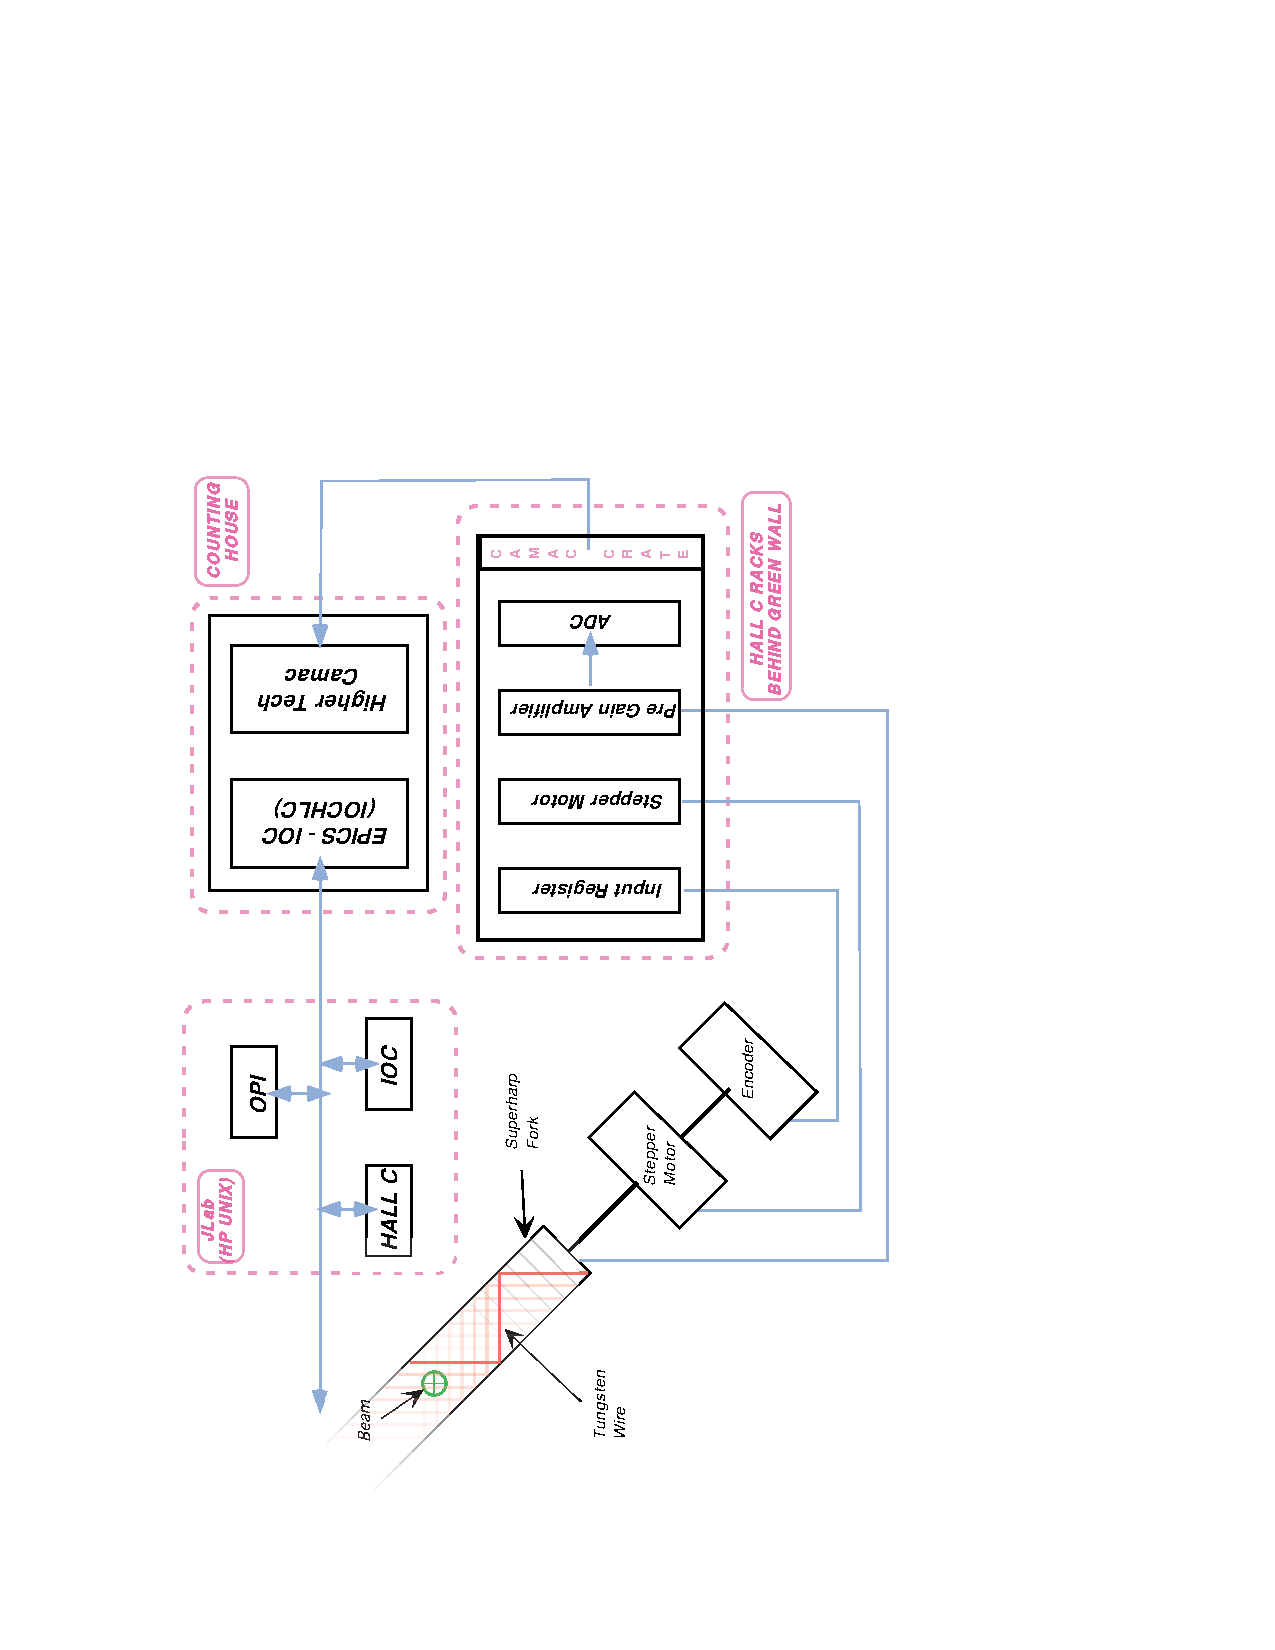
\includegraphics[width=6in,angle=270]{beamline/superharp-system.ps2}
\caption{Schematic of the superharp system.}
\label{figure:superharp}
\end{center}
\end{figure}

The horizontal and vertical positions of the beam are then determined by collecting the charges
produced as the wires go through the electron beam within an accuracy of about 
%!!! $\pm 50~\mu$m
(see Fig.~\ref{figure:interface} in section~\ref{interface}). While the superharp fork
is travelling inside the beam pipe, three diferent signals appears due to the interaction
between the JLab beam and each of the three wires. The time duration during a scan is
approximately 30~sec from the starting rest position to the maximum allowed travel distance
(about 3''=7.62~cm).

The signals are then sent to an Analog Digital Converter (1881-ADC) electronic card and then transfered
to a computer for data analysis. Due to the interaction beam-wires, this device spreads the beam
(destructive method). In addition, with the information on the horizontal position inside the arc, the
energy of the electron beam can also be monitored~\cite{Gueye-98-energy}. This feature will be described
later in section~\ref{analysis}. The current range for these wires is
between 1 and 30~$\mu$A.  

Since some experiments in hall C will run with a current below
1~$\mu$A,  some BLMs have been added to the
current electrode channels.

The Beam Loss Monitor (BLM) is a photo-multiplier tube (Hamamatsu-931B, side cathode) which detects
particles produced when the wires from the superharp's fork interacts
with the  electron beam. Each
superharp has one BLM located downstream about 10~cm (target) and
0.5-2~m ( hall C arc). Combined with
the electrode channel, the total current range of a single superharp device is
$0.01 < I~(\mu {\rm A}) < 30$.

\paragraph{The superharp interface window}\label{interface}

The automated hall C superharp interface window program allows control of both
data acquisition and data analysis. The flow chart of the code is shown on Fig.~\ref{figure:flow_chart}. 
Each superharp device is controlled via 
\htmladdnormallinkfoot{EPICS}{http://epics.aps.anl.gov/asd/controls}. The
signals obtained from a scan are then
stored into an ASCII file which serves as an input file for a {\tt C++} routine where all the
calculations are performed. The main interface window is shown on Fig.~\ref{figure:interface}.

\begin{figure}[!hbt]
\begin{center}
%\htmlimage{thumbnail=0.5,scale=1.0}
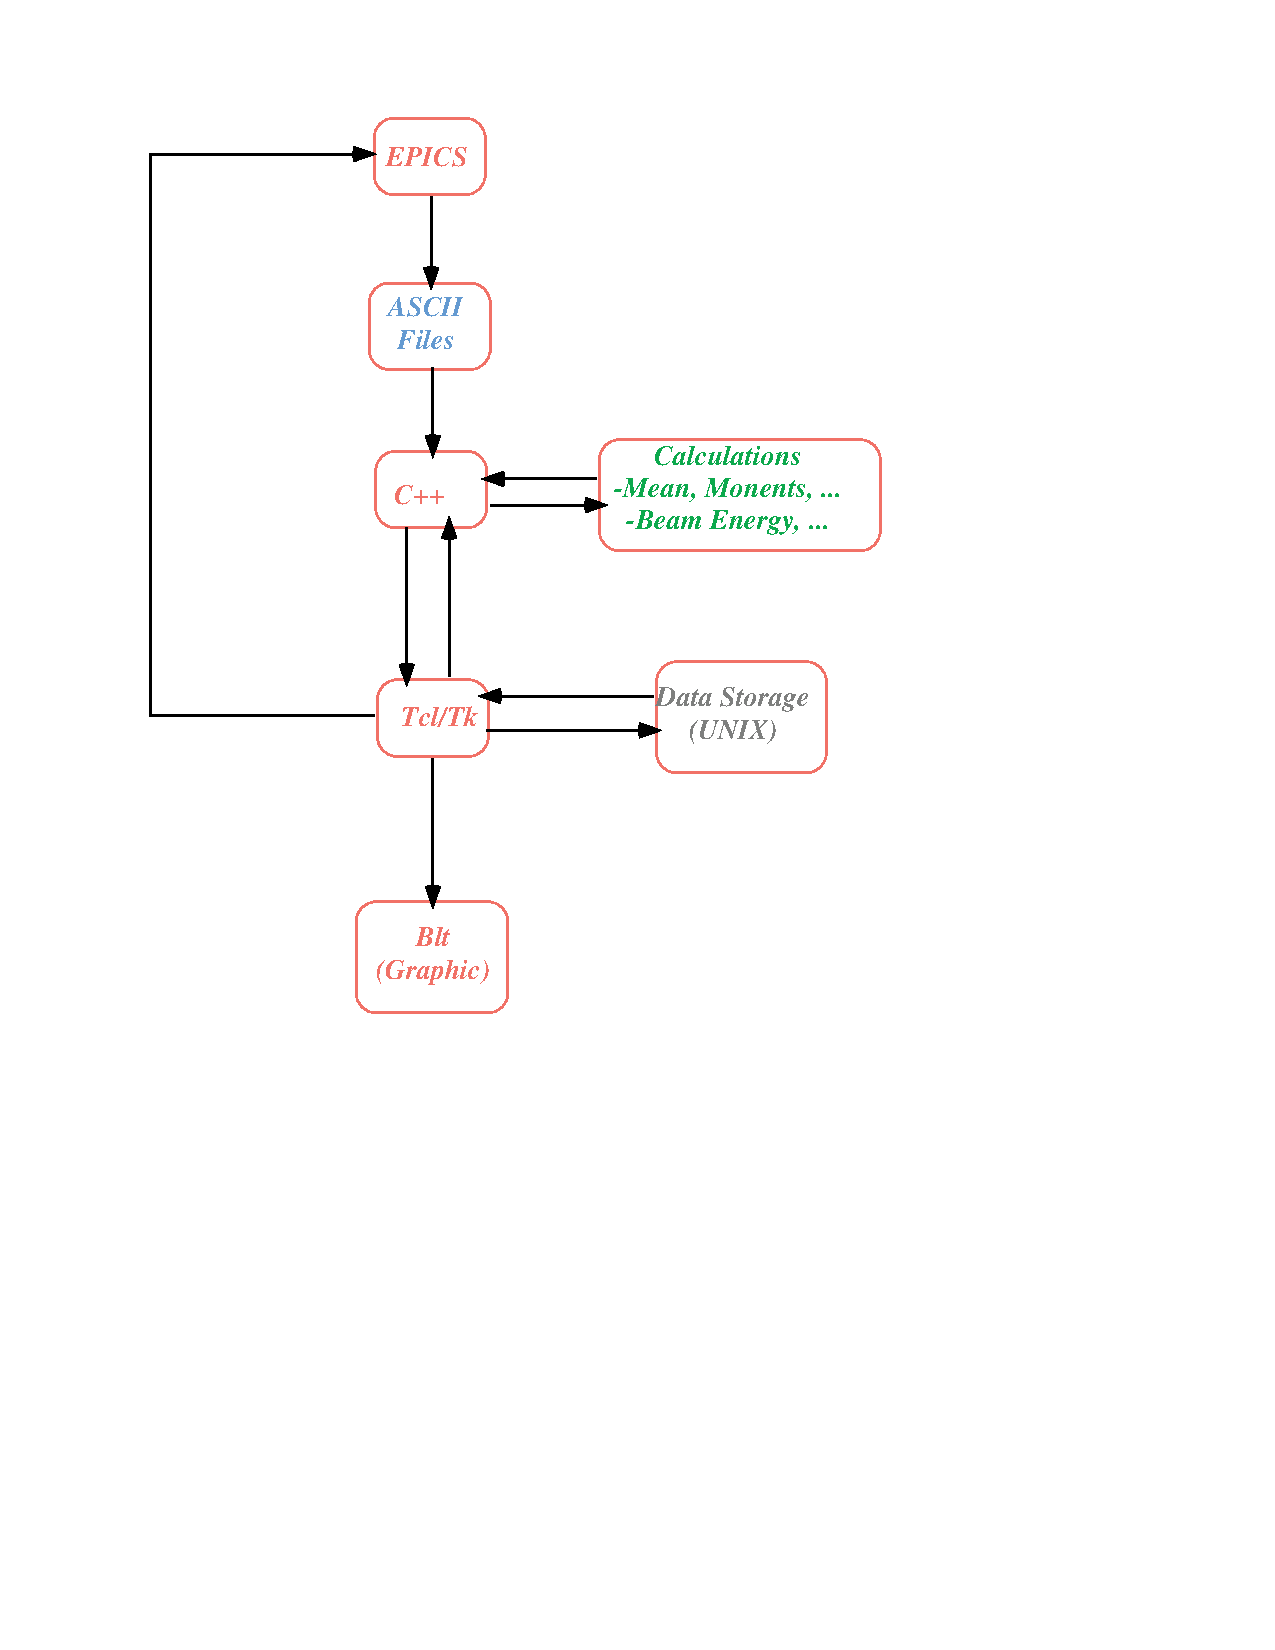
\includegraphics{beamline/superharp-flowchart.ps2}
\caption{Flowchart of the hall C superharp interface program.}\label{figure:flow_chart}
\end{center}
\end{figure}

%%note: natural size of following figure is 7wx8.85h inches.
\begin{figure}[!hbt]
\begin{center}
%\htmlimage{thumbnail=0.5,scale=4.0,flip=r270}
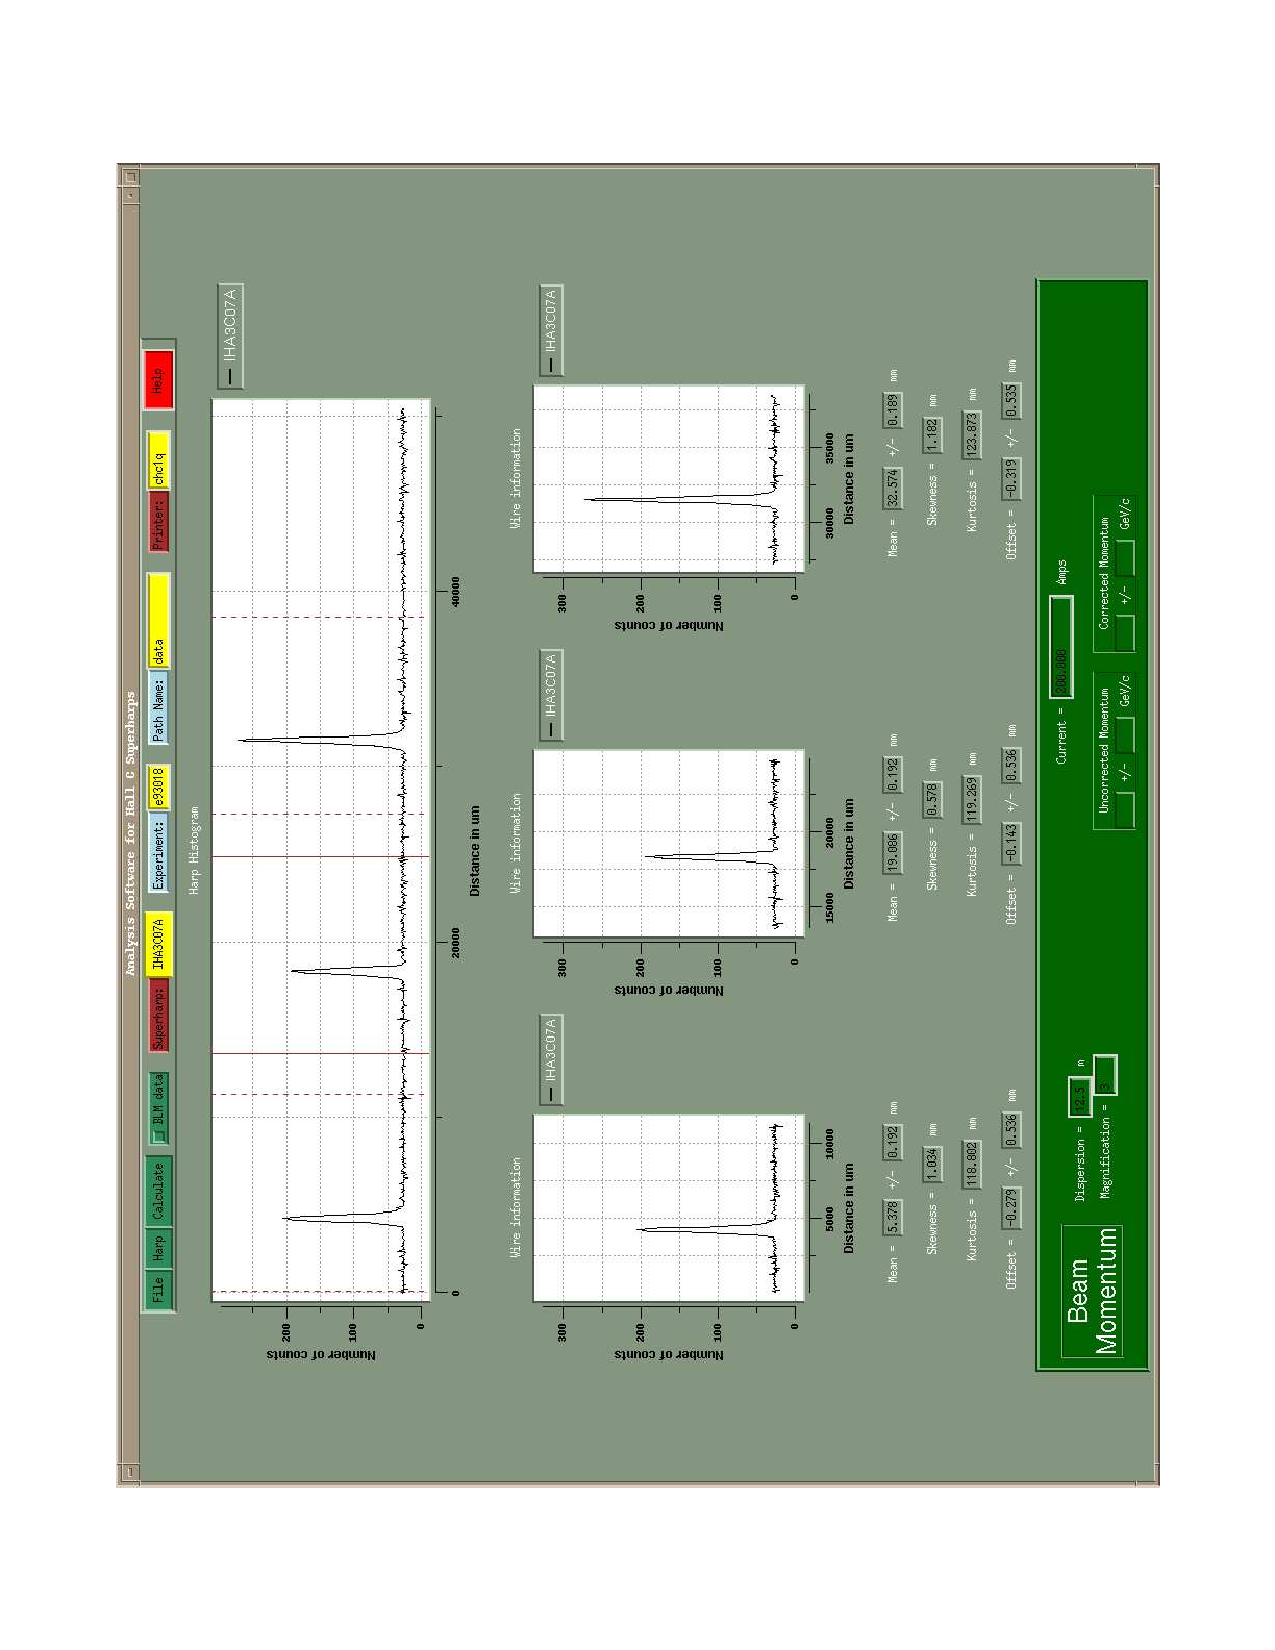
\includegraphics[height=6.5in,width=5.5in]{beamline/superharp_interface.ps2}
\caption{The hall C superharp interface window.}\label{figure:interface}
\end{center}
\end{figure}

In this section, we will review the different menu items that allow users to perform a scan and
perform data analysis.

	\subparagraph{Data Acquisition}\label{daq}

The corresponding code is running only on the actual {\bf cdaqh1} cluster located in the experimental
hall C counting house. Selecting {\bf\fbox{Harp $>$ Scan}} launches the {\tt MEDM} executable routine.

There are two control panels: one allows the user to select the appropriate superharp
(Fig.~\ref{figure:choose_harp}) and one to perform the scanning process (Fig.~\ref{figure:scan_harp}).

\begin{figure}[!hbt]
\begin{center}
%\htmlimage{thumbnail=0.5,scale=2.0}
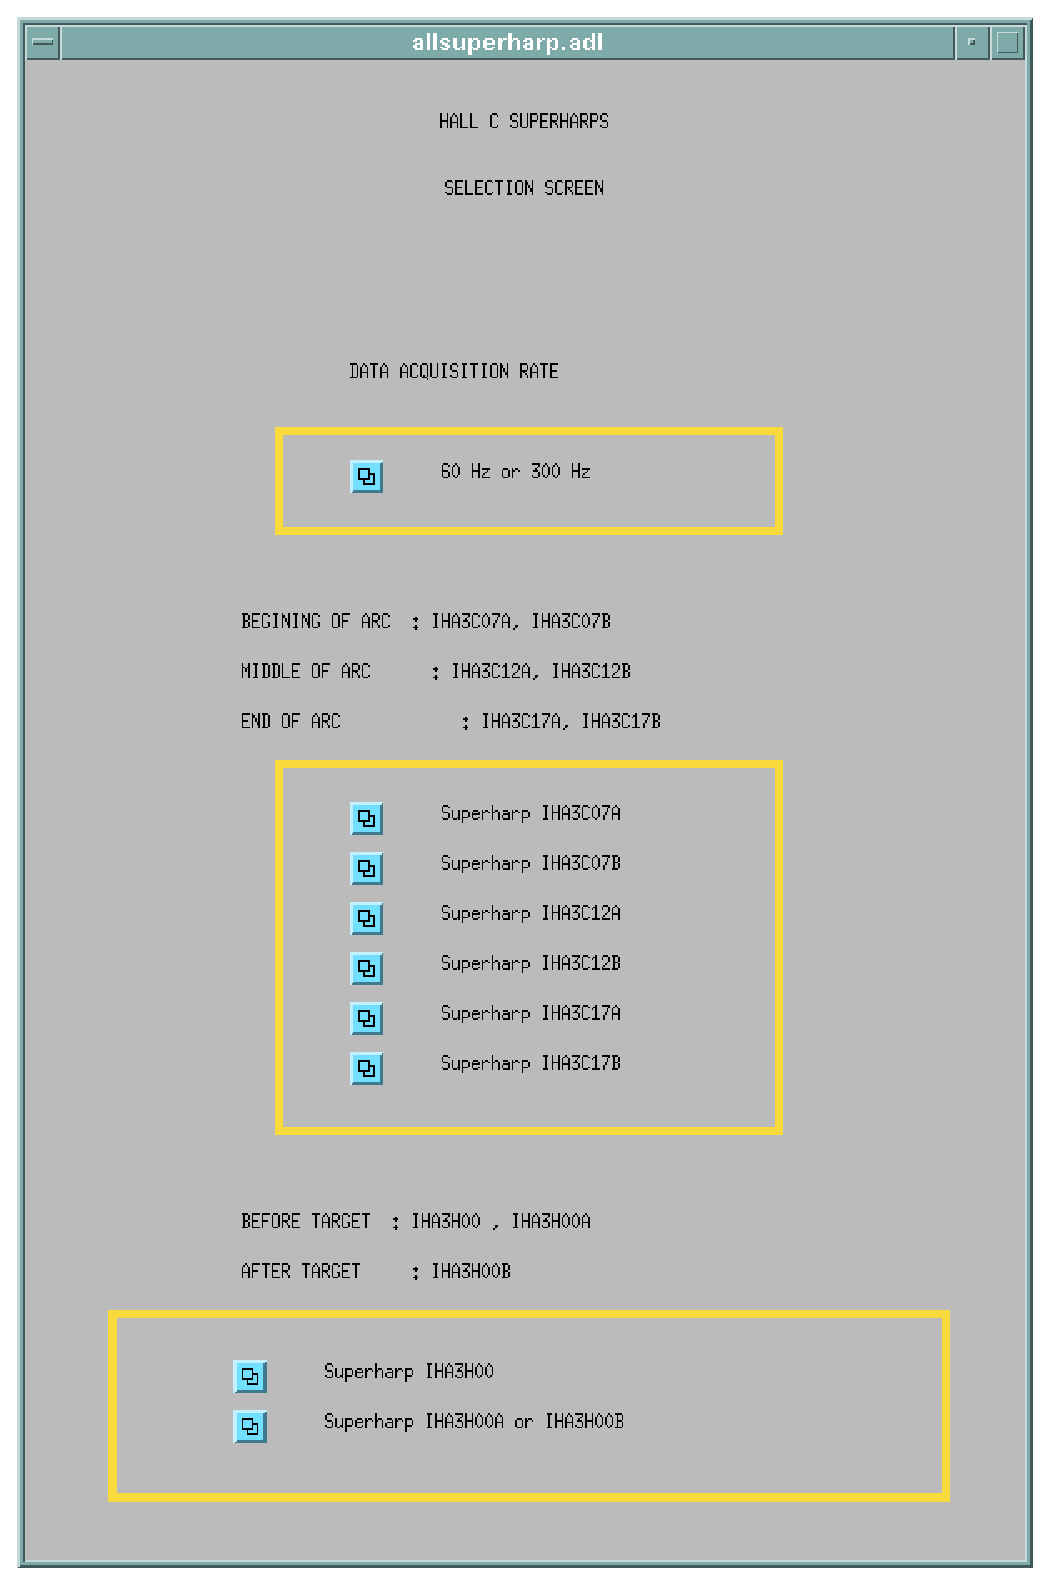
\includegraphics[height=7.2in]{beamline/superharpChoicePanel.ps}
\caption{The hall C superharp selection control panel.}\label{figure:choose_harp}
\end{center}
\end{figure}


\begin{figure}[!hbt]
\begin{center}
\includegraphics{beamline/scan-panel.eps}
\caption{The hall C superharp scanning control panel.}\label{figure:scan_harp}
\end{center}
\end{figure}

Before starting any scanning process, verify that you have the correct default parameters as shown in
Table~\ref{table:scan_harp} below.
\begin{table}[!hbt]
\begin{center}
\begin{tabular}{llr}
\hline
\hline
{\it Values:}			&	\\ 
Acceleration			& 2000~tr/min	\\
Velocity			& 20000~tr/min	\\
Deceleration			& 2000~tr/min	\\
Pre-Gain Amplifier (PGA)	& 2	\\
\hline
\hline
{\it Messages:} 		&	\\
State				& 1	\\
Status				& Declared Zero Point Harp Position \\
Input Register			& 64335 \\
Analog Digital Converter (ADC) counts& 10-30 (background) \\
Cmd Readback			& 129	\\
\hline
\hline
\end{tabular}
	\caption{The default scan parameters for the hall C superharp system.}
	\label{table:scan_harp}
\end{center}
\end{table}
If not, then enter the correct value(s) and hit {\bf\fbox{return}}. Note that the value will {\bf not}
change  unless you hit \fbox{\bf return}. The last two digits in the
{\bf\fbox{Input Register}} box may
not be the same due to the 10~$\mu$m accuracy of the encoder.

After launching {\tt MEDM}, click on the red {\bf\fbox{SCAN}} button to begin the scan. The list
below describes the  change in several important variables during the scanning process.
\begin{enumerate}
\item \fbox{{\bf State}} changes from 1 to 4.
\item \fbox{{\bf Status}} indicates {\it Harp is moving}, {\it Harp is retracting}, and
	{\it Declared zero harp position} during the corresponding motion of the harp.
	{\it Declared zero harp position} indicates that the scan is finished and the harp has
	returned to its fully retracted rest position.
\item \fbox{{\bf Velocity}} changes to 30000~tr/min when the harp comes back.
\item \fbox{{\bf ADC}} registers the number of electrons picked up when a wire crosses the beam.
\item \fbox{{\bf Cmd Readback}} reads {\bf 66} when the harp is moving in the forward direction
	and {\bf 65} in the backward direction.
\end{enumerate}


	\subparagraph{Data analysis}\label{analysis}

Although \fbox{\bf harp\_ana\_new} is the main executable, the files \fbox{\bf harp\_ana\_new.tk}
and \fbox{\tt bltwish} are both required: \fbox{\bf  harp\_ana\_new.tk} contains the graphical routines
for the program and is interpreted at run-time through \fbox{\bf bltwish}. \fbox{\bf harp\_ana\_new} contains
both {\tt C++} and {\tt Tcl/Tk} codes: \fbox{\bf harp\_ana\_new} is written in {\tt C++} and contains most
of the calculation routines, and \fbox{\bf  harp\_ana\_new.tk} is written in {\tt Tk} and contains the user
interface and graphing routines.

	\subparagraph{Menu and entry Items}

The menu commands and entry items are described in Table~\ref{table:menu_entry}.
\begin{table}
\begin{center}
\begin{tabular}{||l|c|l||}
\hline
\hline
\multicolumn{3}{|c|}{\bf Menu Commands and Accelerator}	\\
\hline
File Reset & Ctrl-R & Clears all graphs and removes all data. \\
File Load  & Ctrl-L & Load all data in the current path. \\
File Save  & Ctrl-S & Saves all data in the current path. \\
File Print & Ctrl-P & Prints all graphs to the current printer.\\
File Quit & Ctrl-Q & Exits the program. \\
\hline
Harp Options & & Calls the configuration dialog. \\
Harp Scan & & Launches the medm scanning routine. \\
\hline
Calculate dP/P0 & & Calculates $P$ and $\Delta P$ based on the current data. \\
Calculate Smooth & Ctrl-M & Filters out background noise in all graphs. \\
Calculate Unsmooth & Ctrl-U & Reverses Calculate Smooth. \\
Calculate Transform & Ctrl-T & Calculates the Fourier cosine transform \\
		& & of the data. \\
\hline
\hline
\multicolumn{3}{|c|}{\bf Entry Items}	\\
\hline
Superharp	& & Load the selected superharp from the path	\\
		& & listed in the {\it File Name} entry and graphs it		\\
Experiment	& & Specifies the number of the current experiment.	\\
		& & The destination for files created by File Save 	\\
		& & is {\tt scan\_data/}{\it{Experiment}}{\tt /}{\it File Name}	\\
File Name	& & Specifies the location of the harps to be loaded	\\
		& & or the destination for the files created			\\
		& & by File Save			\\
Printer		& & Specifies the current printer				\\
\hline
\hline
\end{tabular}
	\caption{Definition of the menu commands, accelerators and entry items.}\label{table:menu_entry}
\end{center}
\end{table}

	\subparagraph{Help and BLM data}

The two remaining buttons on the superharp interface window menu bar, \fbox{{\bf BLM data}} and
\fbox{{\bf Help}}, allow users to switch to the BLM channels and displays this document ({\tt harphelp.ps}),
respectively.

\paragraph{Using the Program}\label{program}

This section describes in detail how to use harp\_ana\_new to execute common commands.

	\subparagraph{Loading Old Harp Data}

Data is loaded by selecting the name of the harp from the {\it Superharp} drop-down menu.  The program
looks in the path {\tt scan\_data/}{\it Experiment}{\tt /}{\it File Name}, where {\it Experiment} is
the experiment number listed in the {\it Experiment} entry and {\it File Name} is the file name listed
in the {\it File Name} entry.

	\subparagraph{Loading New Harp Data}

Data collected through Options Scan is automatically converted into a format readable by
{\fbox{\bf harp\_ana\_new}}, so it can been loaded, even in the same session in which it was collected,
as if it were old harp data.

	\subparagraph{Graphing Old Harp Data}

Harp data is automatically graphed when loaded (by selecting it from the {\it Superharp} drop-down menu).
The statistical information for the first graph loaded is also displayed.

	\subparagraph{Graphing New Harp Data}

Connect to {\tt cdaqh1} and run \fbox{\bf harp\_ana\_new}.  Select \fbox{Options Scan}, and follow the
instructions in the {\tt MEDM} section to scan in new data.  After exiting {\tt MEDM}, the new data should
appear. Note that it takes about 10 to 15 seconds for {\tt MEDM} to load.

	\subparagraph{Saving Harp Data}

Selecting \fbox{File Save} saves and compresses (using {\tt gzip}) the data for all the harps
currently loaded in the directory {\tt scan\_data/}{\it Experiment}{\tt /}{\it File Name}, where
{\it Experiment} is the experiment number listed in the {\it Experiment} entry and {\it File Name}
is the file name listed in the {\it File Name} entry.  If the directory {\tt scan\_data/}{\it Experiment}
does not already exist, it is automatically created.

	\subparagraph{Printing Harp Data}

Selecting \fbox{File Print} prints a screen capture to the printer listed in the {\it Printer} entry.

	\subparagraph{Removing Harp Data}

Selecting \fbox{File Reset} clears all harp data from the screen and from memory (but doesn't
erase the files from disk).


	\subparagraph{Fourier Transform}

It has been demonstrated that the JLab beam has a fundamental 60~Hz motion originating from the power
line. In order to have a precise determination of the position of the beam, correction from this beam
motion is necessary. For that purpose, a Fourier transform which returns the beam motion harmonics to
all orders from the data has been developped.

Selecting \fbox{Calculate Transform} calls the dialog box displayed in Fig~\ref{fig:transform}.
\begin{figure}[htp]
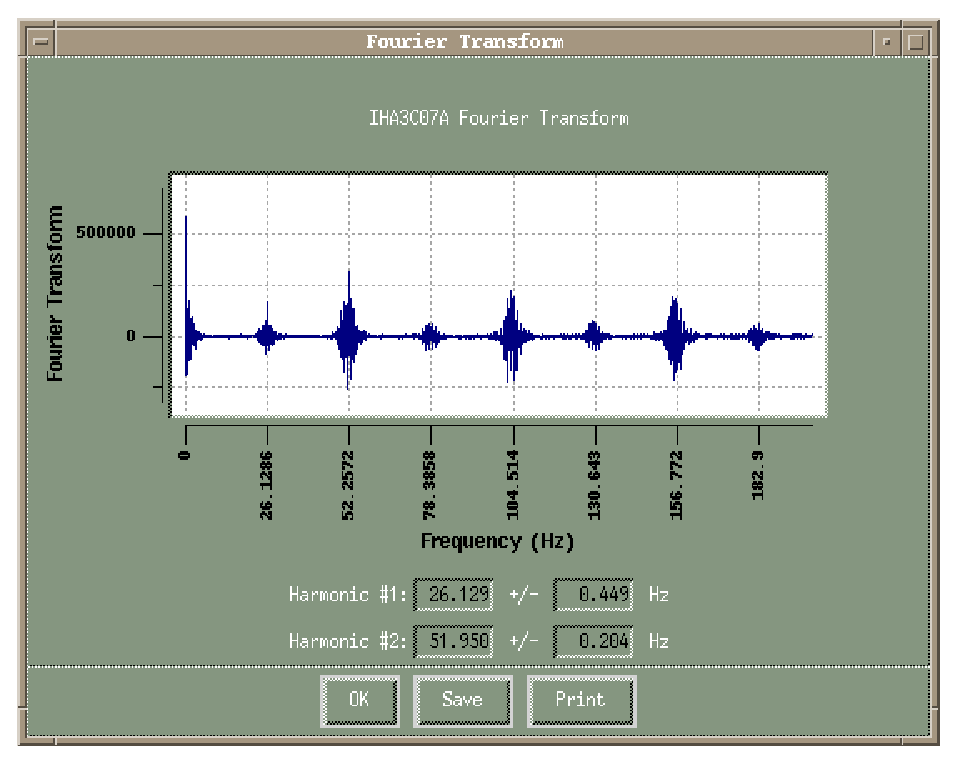
\includegraphics{beamline/fourier_transform.ps}
\caption{The Fourier transform interface.}\label{fig:transform}
\end{figure}
The Fourier transform used to isolate the fundamental frequency of the beam is
\begin{equation}
\hat f(t)=\int_{-\infty}^\infty f(s)\cos \frac{2 \pi s t}{v} {\rm d}x,
\end{equation}
where $v\approx 0.248\mu m/s$ is the speed of the encoder.  Let $N(x)$ be a continuous interpolation of
the harp data, so that $N(x)$ equals the electron count $n_i$ at each of the data points $(x_i, n_i)$ and
0 off the scanning region $(x_{min}, x_{max})$. Then
%\begin{eqnarray}
%\hat N(s)&=&\int_{-\infty}^\infty N(x)\cos \frac{2 \pi s t}{v} {\rm d}x \\
%	&=&\int_{x_{min}}^{x_{max}} N(x)\cos \frac{2 \pi s t}{v} {\rm d}x \\
%	&\approx& \frac{\Delta x}{3}\sum_{i<i_{max}} c_i n_i(x_i) \cos \frac{2 \pi x_i s}{v},
%\end{eqnarray}
%Ed. Note: the above eqnarray was reformatted below for compatibility with latex2html.
\begin{center}
\begin{equation}
\begin{tabular}{rcl}
$\hat N(s)$&$=$&$\int_{-\infty}^\infty N(x)\cos \frac{2 \pi s t}{v} {\rm d}x$ \\
	   &$=$&$\int_{x_{min}}^{x_{max}} N(x)\cos \frac{2 \pi s t}{v} {\rm d}x $\\
	   &$\approx$&$ \frac{\Delta x}{3}\sum_{i<i_{max}} c_i n_i(x_i) \cos \frac{2 \pi x_i s}{v}$,
\end{tabular}
\end{equation}
\end{center}
where $\Delta x=x_{i+1}-x_i,$ $i_{max}$ is an arbitrary large constant, and the $c_i$ are the constants given
by Simpson's integration method.

By Poisson's summation formula, 
\begin{equation}\label{poisson}
\sum_{n=1, 2,\ldots} \hat f(n\omega) =
	\frac{1}{2\omega}\sum_{n=1, 2, \ldots} f\left(\frac{n}{\omega}\right).
\end{equation}
The algorithm used to isolate the fundamental frequency $\omega_0$ of the beam essentially attempts to
maximize the sum (\ref{poisson}).

	\subparagraph{Statistics calculations}

	{\sl Mean and FWHM}

For each superharp scan, the resulting histogram peak centroids are computed using the equation:
%\begin{eqnarray}
%\overline{x}	& = & \frac{\sum \omega_i x_i}{\sum \omega_i}	\\
%\omega_i	& = & \frac{\sqrt{\sum (\Delta n_i)^2}}{n_i} = \frac{\sqrt{\sum n_i}}{n_i} \; ,
%\end{eqnarray}
\begin{center}
\begin{equation}
\begin{tabular}{rcl}
$\overline{x}$&$ = $&$ \frac{\sum \omega_i x_i}{\sum \omega_i}	$\\
$\omega_i    $&$ = $&$ \frac{\sqrt{\sum (\Delta n_i)^2}}{n_i} $\\
              &$ = $&$ \frac{\sqrt{\sum n_i}}{n_i} $\ ,
\end{tabular}
\end{equation}
\end{center}
\noindent
where $n_i$ is the number of counts at the position $x_i$. $\sum n_i$ represents
the total number of events in the selected peak. The beam position is then calculated via:
\begin{equation}
x_{\rm beam} = \overline{x} - x_{\rm survey} \; ,
\end{equation}
where $x_{\rm survey}$ corresponds to the location of each wire if the beam was along the
ideal path inside the beampipe.

The standard deviation (rms) is calculated from the second moment (variance) of the
distribution:
\begin{equation}
M_2 = \sigma^2 =
	\sqrt{\frac{1}{\sum n_i-1}\frac{\sum \omega_i (x_i-\overline{x})^2}{\sum \omega_i}} \; ,
\end{equation}
and the full width at half maximum (FWHM) from:
\begin{equation}
\sigma = \frac{FWHM}{2\sqrt{2ln2}} \; .
\end{equation}

	{\sl Skewness and Kurtosis}

Statistical higher moments $M_n$ are also calculated:
\begin{equation}
M_n = \frac{\sum \omega_i (x_i-\overline{x})^n}{\sum \omega_i} \; , \; {\rm for \; n>2} \; .
\end{equation}
Since the term $1/(\sum n_i-1)$ appears in $\sigma=\sqrt{M_2},$ most statistical calculations
are also normalized.  

The skewness is defined as the measure of the symmetry of a distribution:
\begin{equation}
B_1=\frac{M_3}{M_2^\frac{3}{2}} \; .
\end{equation}
It vanishes for any distribution completely symmetric about its mean (since this forces $M_n$ to 
vanish for odd $n$), and so vanishes for the normal distribution.

The kurtosis is the measure of a distribution's spread about its mean:
\begin{equation}
B_2=\frac{M_4}{M_2^2}-3
\end{equation}
It also vanishes for a normal distribution, since $M_4=3\sigma^2$ and $M_2=\sigma.$

	\subparagraph{Graph Comparisons}

Using survey data, the program isolates the three peaks of the first graph $H_0$ loaded and plots them in the
three lower graph windows.  As subsequent graphs $H_i$ are loaded, the offset
$\overline{x_{H_i}}-\overline{x_{H_0}}$ is calculated over each of those three regions and displayed in the 
upper-right corner of the appropriate graph.  The offsets have the same order and color as the harp names in
the graph legend.
 
When data from both of a pair of harps (e.g. IHA3C17A and IHA3C17B) are loaded, the angle $\theta$ the
beam makes with the horizontal when travelling through the pair is calculated and displayed.  As with the
offsets, the color of the displayed angle matches the color of graph of the harp pair.

\paragraph{Beam energy measurement}\label{energy}

After loading the data from the superharps at the entrance (IHA3C07A and IHA3C07B) and at
the exit (IHA3C17A and IHA3C17B) of the hall C arc beamline, 
the \fbox{Calculate dP/P0} option
will be enabled?  This menu option allows users to calculate the beam incident energy through some
conditions:
\begin{enumerate}
\item If the full width of the first peak of harp IHA3C07A is less than twice the full
width of the first peak of harp IHA3C17A, then the beam is not dispersive enough to perform the
calculation, and an error will be generated.
\item Prior to the calculation, one has to verify the dispersion and the amplification factor at the
exit of the arc related to the hall C beamline optic settings. The default values are now 12.5~cm and 3,
respectively.
\item {\bf Only the MCC operators are allowed to perform the beam energy calculation since there is a setup
procedure to follow~\cite{ebeam_proc99} (see
appendix~\ref{append_ebeam_proc99})}.  The users can
re-evaluate this calculation by asking for the setting current of the arc dipole magnets and loading all
the corresponding superharp data.
\end{enumerate}

The basic idea behind the calculation is as follows.
Suppose a particle with mass $m$ and charge $q$ is subjected to a magnetic field $\vec{B}$ perpendicular
to the plane of the particle's motion, causing it to travel in a circular path of radius $R$. The beam
momentum $P_0$ is determined via:
\begin{equation}
P_0 = \frac{e}{\Theta}\int Bdl
\end{equation}
where $\int Bdl$ is the magnetic field integral over the path of the electron beam and
$\Theta = 34.3^\circ$ is the bending angle through which the electron beam is deflected. $\int Bdl$ is
determined by mapping bending magnets absolutely with a combination of NMR and Hall probes. Taking $e$
as a constant, this leads to the uncertainty relation:
\begin{equation}
\frac{\Delta P}{P_0} = \sqrt{\Big (\frac{\Delta \int Bdl}{\int Bdl}\Big )^{2}
                     + \Big (\frac{\Delta \Theta}{\Theta}\Big )^{2}} \; .
\end{equation}

The inclusion of the beam incident angle is taken into account by utilizing the Lorentz force:
\begin{equation}
\vec{F}=-e\vec{v}\times \vec{B} = m_e\vec{a},
\end{equation}
where $\vec{a}$ is the acceleration and $m_e$ the mass of the electron. Projecting on the three cartesian
axis (z-beam direction, x-transverse horizontal and y-transverse vertical):
\begin{equation}
\left \{
\begin{array}{lll}
a_x & = & -\frac{evB}{m_e} 	\\
a_y & = & 0			\\
a_z & = & 0			\\
\end{array}
\right .
\Leftrightarrow
\left \{
\begin{array}{lll}
v_x & = &  -\frac{evB}{m_e}t + vsin(\theta _x)	\\
v_y & = & vcos(\theta _y)				\\
v_z & = & vcos(\theta _x)				\\
\end{array}
\right .
\end{equation}

\begin{equation}
\Leftrightarrow
\left \{
\begin{array}{lll}\label{eq:txy}
x & = &  -\frac{evB}{2m_e}t^2 + vsin(\theta _x)t + x_0	\\
y & = & vcos(\theta _y)t + y_0				\\
z & = & vcos(\theta _x)t + z_0				\\
\end{array}
\right .
\end{equation}
We are in a case where: $z_0 = 0$. Therefore:
\begin{equation}
\left \{
\begin{array}{lll}
t & = & \frac{z}{vcos(\theta_x)}					\\
x & = & -\frac{eB}{2m_evcos^2(\theta _x)}z^2 + tan(\theta _x)z + x_0	\\
y & = & \frac{cos(\theta _y)}{cos(\theta _x)}z + y_0			\\
\end{array}
\right .
\end{equation}
The system in (\ref{eq:txy}) characterizes the trajectories of the particle along
$x$ and $y$ as a function of its position inside the magnetic region along $z$.

The expression of $x$ represents the trajectory of the particles in the dispersion plane
(where the particles are subject to the magnetic field):
\begin{equation}
x = -\frac{eB}{2Pcos^2(\theta _x)}z^2 + tan(\theta _x)z + x_0,
\end{equation}
where $x = x_{17}$, $x_0 = x_{07}$ and $\theta _x = \theta _{07}$ are determined by using the superharps
at the entrance (IHA3C07) and at the exit (IHA3C17) of the arc. The beam momentum $P$ corrected from
incident beam angle can then be evaluated.

\paragraph{Further Help}

For further assistance, contact
\par
\noindent
\begin{table}[!ht]
\begin{tabular}{l}
Paul Gu\`eye \\
e-mail: {\tt gueye@jlab.org} \\
Phone: (757) 269-7167 \\
Pager: (757) 849-7167 \\
\end{tabular}
\end{table}



\subsection{M\o ller Polarimeter }
The M\o ller Polarimeter is used to measure the electron beam
polarization. Instructions for carrying out such a measurement
are documented in a 
\htmladdnormallinkfoot{Step-by-Step Guide}{http://www.jlab.org/Hall-C/document}.
MCC follows a complementary 
\htmladdnormallink{procedure}{http://opsntsrv.acc.jlab.org/ops_docs/online_document_files/MCC_online_files/HallC_Moller_pol_measurement_proc.pdf}.
The polarimeter is located at the beginning of the Hall C
alcove downstream of the granite table that holds the super-harps.
All magnetic elements of the polarimeter are located between
the BPMs 3C17 and 3C18: there are a solenoid and two quadrupoles.
The M\o ller target is located in the center of the solenoid. The
detectors are positioned 11 meters downstream of the target and 0.49
meters away from the beam line in a lead house.

The Hall~C M\o ller polarimeter consists of: the target and target solenoid, the quadrupole magnets, a 
collimator box, and the detectors.  These are described in turn in 
the paragraphs below:

{\sl Target Solenoid} This is a $\approx$ 3 T super conducting
solenoid used to ``brute force" polarize the valence electrons in a
thin, $\approx$ 10 $\mu$m, iron foil perpendicular to the
plane of the foil. This magnet has a liquid nitrogen cooled radiation shield
and requires liquid helium for operation.

{\sl Quadrupole Magnets} In order to keep the locations of the M\o ller
target and detectors fixed regardless of the incident beam energy
a two quadrupole optics was chosen. The first quadrupole (``the Los Alamos Quad")
has a 4 inch bore and a physical length of about 1 ft.
The second quadrupole (10Q36) has a 10 inch bore and physical length of 123 cm.

{\sl Collimator Box} There are seven movable blocks of densimet (densimet is
a machinable alloy of tungsten) for the collimator. These blocks form two
horizontal jaw pairs and one vertical jaw pair. The seventh block has a
hole in it through which the unscattered electron beam travels.

{\sl Detectors} The Hall~C polarimeter was built to operate in coincidence
mode with both the scattered and recoiling electrons being detected in
coincidence. There are thus two identical detector stacks placed symmetrically
about the beamline. Each stack consists of a sixteen element hodoscope
followed by a lead glass block.

\paragraph{Polarimeter Description}
The layout of the polarimeter is shown in fig.~\ref{polscetch}.
The incoming electron beam hits an iron target foil. The target thickness
is on the order of 4 to 10 $\mu m$. The electrons in the iron foil
are polarized by the 3 T magnetic field of the super conducting solenoid.
The beam electrons scatter off 
the target electrons (M\o ller Scattering) 
with the scattering angle of interest at about
1$^{\circ}$ or below in the laboratory system. Since the electrons
are very close to the beam line they need to be deflected away from
it in order to be detected in coincidence. This is achieved by
two quadrupoles. The first smaller quadrupole is focusing in the
horizontal plane  while the
second large quadrupole is defocusing in the same plane. The use of two quadrupoles
allows us to keep the cone of the 90$^{\circ}$ CM scattered electrons 
at fixed dimensions after a 11 meter drift distance, namely
49cm horizontal and 16cm vertical from the beam line.
The first quadrupole (the Los Alamos Quad) has a 4 inch bore and a
physical length of 12 inches. The second quadrupole (10Q36) has a 10
inch bore and a physical length of 123 cm.
\begin{figure}[htp]
\begin{center}
\includegraphics[height=4in,width=6in]{beamline/polarimeter.eps}
\caption{Sketch of the M\o ller polarimeter in Hall C.\label{polscetch}}
\end{center}
\end{figure}
The two electrons are detected in coincidence using two lead glass 
shower counters as shown in Figure \ref{detarr}. In front of each counter is a collimator that defines
the acceptance. The right collimator is intentionally larger
than the left. This reduces the sensitivity of the coincidence 
acceptance to beam and detector positions. In front of the collimator
is a hodoscope with 16 channels. Each channel is a scintillator of 1cm
width.
\begin{figure}
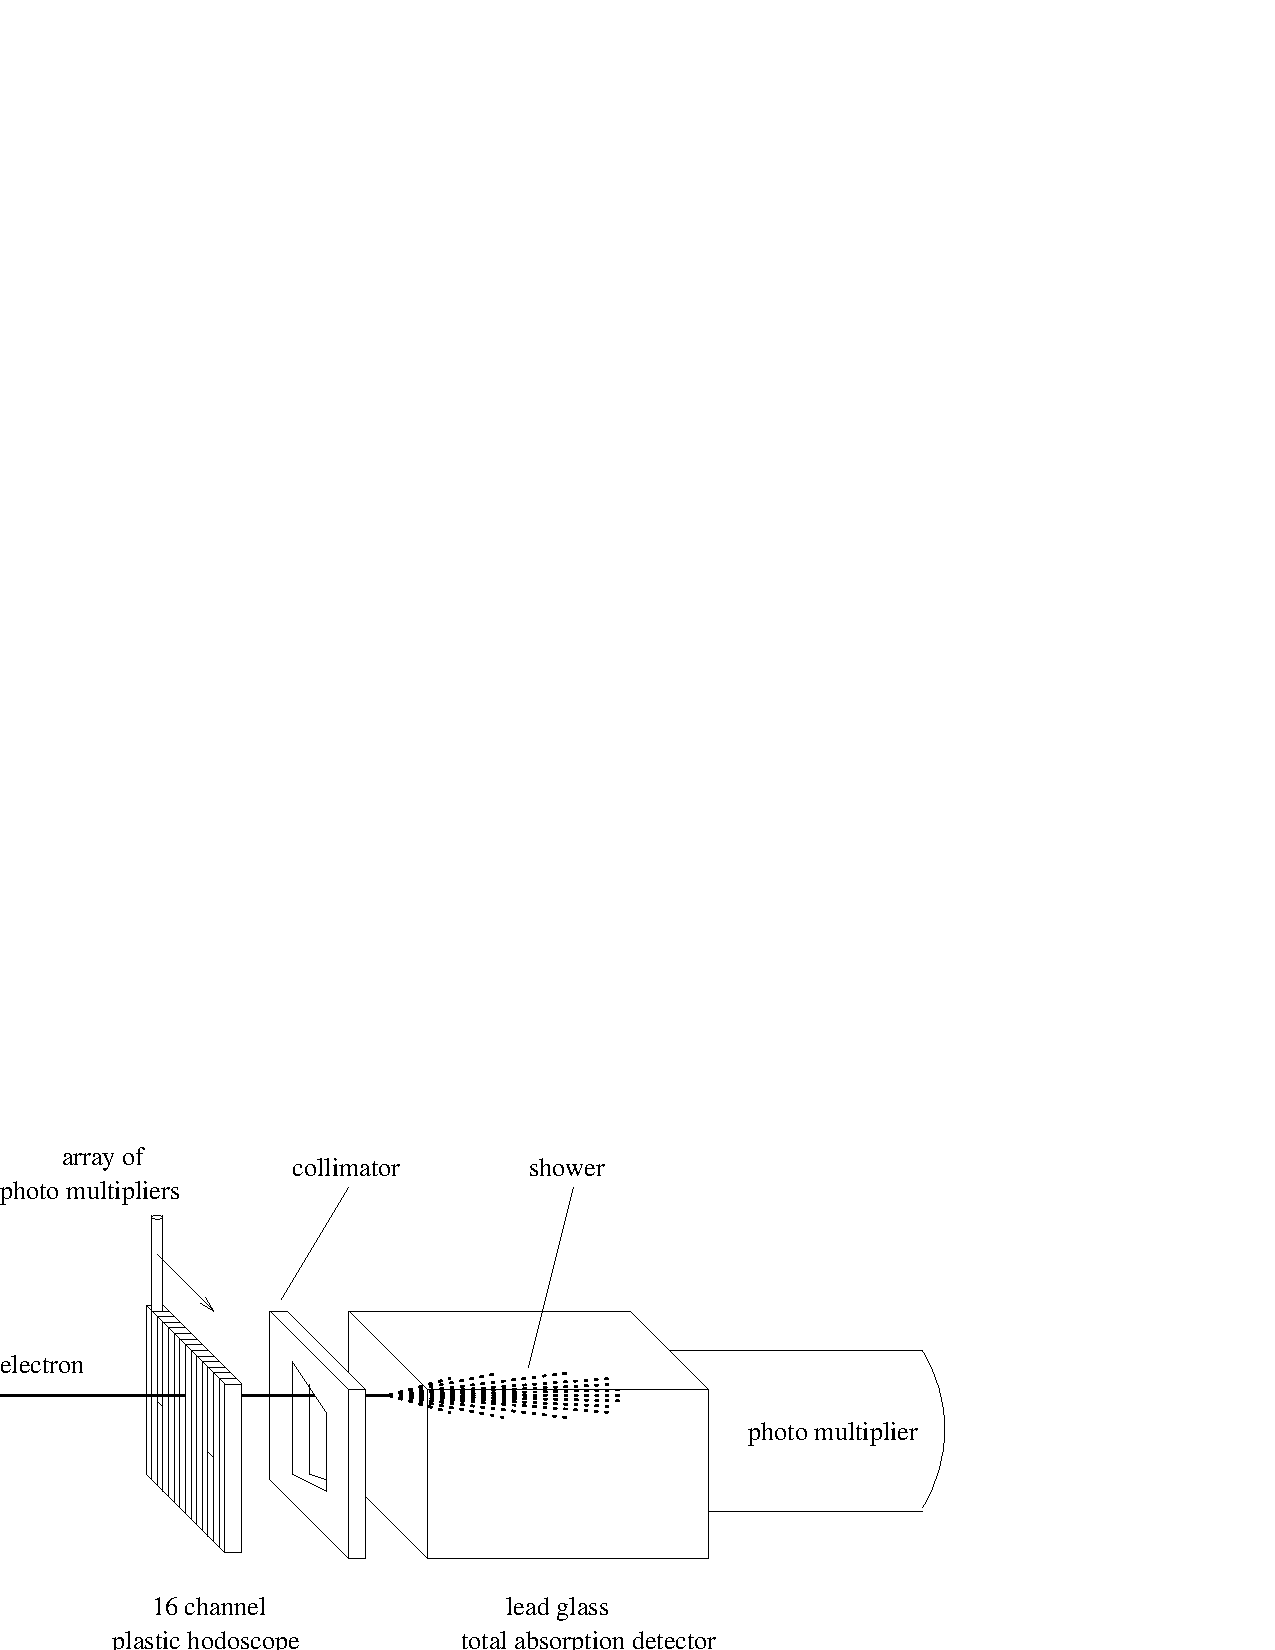
\includegraphics[height=4in,width=6in]{beamline/detarangement.epsf}
\begin{center}
\parbox{10cm}{
\caption{Detector arrangement}\label{detarr}}
\end{center}
\end{figure}

Since the cross section for Mott scattering (electron - nucleus
scattering) is much larger than M\o ller scattering it is necessary
to use collimators to reduce this background that leads to accidental
coincidences. This is achieved with a set of movable collimators
located between the two quadrupoles (see fig.~\ref{polscetch} 
and \ref{colscetch}). 
%
\begin{figure}
\includegraphics[height=4in]{beamline/collim.eps}
\begin{center}
\caption{Collimator with M\o ller trajectories\label{colscetch}}
\end{center}
\end{figure}
Mott electrons with the right momentum and scattering angle that make it
through the quadrupoles into the detectors do not follow the same
path in configuration space as 
the M\o ller electrons do.  The collimators are used to shield the
space that is not transversed by the M\o ller electrons. The space of
the M\o ller stripes is  
given by the collimators in front of the lead glass detectors
that define the coincidence acceptance.
%

\paragraph{M\o ller Control Software and Hardware}
There are three main control packages for the M\o ller Polarimeter.
Two of them are GUIs run from the Hall C Counting Room. They
control 1)~the solenoid cryogenics, and 2)~the solenoid field, 
the target, and the collimators. Control of the two quadrupoles
is possible only from MCC, although the second counting room GUI does
allow experimenters to monitor the quadrupole settings.


\begin{figure}
  \begin{center}
%  \htmlimage{scale=1.0,thumbnail=0.5}
  \includegraphics[height=4in]{beamline/mollergui.ps}
  \caption{M\o ller Polarimeter Control GUI\label{molpolmedm}}
  \end{center}
\end{figure}
%

\subparagraph{Polarimeter GUI}

To run the GUI using medm do the following steps
\begin{itemize}
\item Log onto cdaqh1 from the account {\tt cvxwrks}.
\item Set directory: \begin{verbatim} cd MEDM/moller \end{verbatim}
\item Start the GUI: \begin{verbatim} medme moller.adl  \end{verbatim} 
\end{itemize}
%

\subparagraph{Quadrupole Settings}

Although the quadrupoles are controlled only by MCC, it is the 
responsibility of the experimenter to make certain that they are
set to the correct currents.
The correct currents are a function of the incidentbeam energy . The example currents given in Table \ref{tab_qcurrent} are in Amps
and were determined by tuning the system using beam. The final currents 
are determined experimentally by optimizing the
M\o ller hodoscope left-right correlation. This guarantees that the polarimeter
acceptance is centered around 90 degrees in the center of mass.
%
\begin{table}[!hbt]
\begin{center}
\begin{tabular}{|c|c|c|l|} \hline
Beam Energy & Q1  & Q2 &Reference data \\
\hline
0.884 &  85.9 & 112.0 & March, 2001  \\
2.332 & 136.0 & 364.0 & August, 2001 \\
2.415 & 137.1 & 380.0 & April, 2001  \\
3.395 & 142.2 & 586.0 & March, 2001  \\
\hline 
\end{tabular}
\caption{M\o ller Quadrupole Current Setings\label{tab_qcurrent}}
\end{center}
\end{table}

A reminder to the expert: After a power failure or power cycle of the Q1 
power supply and/or controller,
it is necessary to press the green "START" button on the Q1 (Small
M\o ller Quad) power supply.  If MCC cannot get any real current out of the
supply then probably it is in standby mode and needs the START button pushed.

Currently the Degauss procedure for Q2 is to ramp the magnet up to 800 Amps 
then ramp down to zero, reverse polarity, ramp to -240 Amp and finally
back to zero. This procedure is almost never used and is not known to
be important.

%
\subparagraph{Target Motion}
There are four possible target positions, shown in Table \ref{tab_moltar}. They
can be selected using the GUI  
with the frame title {\tt ``Target Ladder''} . In the menu indicated
by the term {\tt ``Cancel''} the four individual target positions 
can be selected. Once chosen with the mouse pointer the 
target ladder will move! {\bf ALWAYS (BEAM OFF) WHEN TARGET IS BEING MOVED.}
Since the target positions are hardwired in the code, any 
corrections to these values need to be done manually using 
the {\tt ``Jog''} option of the GUI. The camera button {\tt ``ON OFF'' }
turns  the target camera and light on and off respectively.
\begin{table}
\begin{center}
\begin{tabular}{|c|c|c|l|c|} \hline
Target & Material & Thick $mu$m & State & Position \\
\hline
1 & Fe & 4  & polished   & -1.96   \\
2 & Fe & 10 & polished   & -0.48  \\
3 & Fe & 4  & unpolished & +1.00  \\
4 & Fe & 10 & unpolished &  n/a \\
\hline 
\end{tabular}
\parbox{10cm}{
\caption{M\o ller Targets\label{tab_moltar}}}
\end{center}
\end{table}
%
After a power cycle the target first needs to find HOME. This can
be done selecting the {\tt ``HOME''} in the menu. To move the target
ladder fully out of the beam select  {\tt ``RETRACT''} from the menu.
At position -3.86 the target is fully out of the beam.
%
\subparagraph{Collimator Positions}
{\bf Never move collimator 5 while beam is present!!!}\\
{\bf Never issue the Go Home while beam is present!!!}\\
The collimator positions also depend on beam energy. However
this dependency is only small since the collimators do not need
to be located very tight to the M\o ller stripes. The singles rates 
do not increase significantly if the collimators are even 5 mm away 
from the M\o ller stripes. The menu in the GUI for the collimator
control provides three different predefined collimator settings.
These settings can be loaded and executed or the values
can be typed in manually.

Each collimator can be moved individually be typing a value in the 
column {\tt ``SetPoint''}
at the appropriate window, see fig. \ref{molpolmedm}. Use the {\tt ``RETURN''} key
to set the value and the {\tt ``Move''} button to move the collimator
to this value. For the collimators 1,2,3,4,6 the values can not 
be larger than zero because that would move the collimators into the
beam (software cut). The collimator 5 is a special case since the beam goes through
a central hole in the collimator. 
After a power cycle all the collimators need to find the HOME position
first.  This is done by using the {\tt ``Go Home''} menu that pops up
a window to ask if one really want to search the home position. 
%
\subparagraph{Target Solenoid}
Since the target solenoid is super conducting and therefore cooled
with liquid helium the console is somewhat more complicated.
Currently we run the magnet at a field of 3 Tesla. Before ramping
up the magnet, check the helium and nitrogen levels
(see fig \ref{molpolmedm}). The magnet has to be put 
into standby mode first, this turns the heater on.  Use button {\tt ``SDBY''}. 
After 20 seconds one
can ramp up the magnet using the {\tt ``GO SET''} button. This ramps up
the magnet to the field value set in the frame {\tt ``Set Field(Tesla)''}.
After reaching the desired field the magnet can be put into persistent mode 
(i.e. turns off the heater) by hitting the button {\tt ``PRST''}. 
The maximum ramp up speed is 12 Amps per minute. 
However, the first ramp-up after a thermal cycle should be made at
6~amps/minute up to 2.4~T, followed by 3~amps/minute to 3~T.
The power supply has an internal ramp up parameter
that will limit ramping to 4 Amps per minute at higher fields.
The ramp up process can be stopped at any time by hitting the {\tt
``HOLD''} button. \\ \\
After a power cycle the remote button {\tt ``REM''} has to be activated
first in order to establish communication to the power supply.
The power supply is an IPS120-10 from OXFORD. Since it is a polarity
reversible device the sign of the field value chosen by the
{\tt ``Set Field(Tesla)''} is important. To reverse polarity the magnet
needs to be ramped down to zero first.
%


\newpage
\subparagraph{M\o ller Cryogenics GUI}
The liquid nitrogen and helium supplies are monitored and controlled by
a GUI with the drivers running on the IOC vmec10 (aka {\it iochc10}).
A screen snapshot is shown in Figure \ref{molcryomedm}.
To run the GUI using medm, perform the following steps:
\begin{itemize}
\item Log onto cdaqh1 from the account {\tt cvxwrks}.
\item Set directory: \begin{verbatim} cd MEDM/Moller/CRYO \end{verbatim}
\item Start the GUI: \begin{verbatim} medme hcmcryo.adl  \end{verbatim} 
\end{itemize}

\begin{figure}
\begin{center}
\includegraphics[height=4in]{beamline/molcryogui.ps}
\caption{M\o ller Cryo GUI\label{molcryomedm}}
\end{center}
\end{figure}
%

Normally, the cryogen levels in the solenoid cryostat should be
automatically maintained at or above 60\% by the controls software.
If mandated, you may turn off the supply of helium or nitrogen by
closing JT-valves {\tt EV91017} or {\tt EV91018}, respectively.

Note that if VMEC10 (iochc10) gets rebooted, it is necessary to RESTORE the cryo valve
parameters for the M\o ller. You do this by clicking on the small blue box on the
bottom of the cryo overview screen (hcmcryo.adl), selecting "SAVE/RESTORE",
then selecting "iochc10:NORMAL RESTORE" from the "!" box in the resulting
screen. It will prompt you to hit ENTER several times. Do so until the dialog
window goes away.

Cooling down the magnet from room temperature should only be done
by a M\o ller cryo expert. The steps are
\begin{enumerate}
	\item Close {\tt EV91019} to isolate the cold return line.
	\item Open {\tt EV91018} to about 35\% and flow nitrogen at this rate
		until the nitrogen level indicator shows liquid in the cryostat.
		This may take several hours. (You may start precooling the helium
		lines [below] at the same time.)
	\item Using the submenu pushbutton for {\tt EV91018}, put the valve on
		PID control. PID parameters should be:
	\begin{enumerate}
		\item Max Pos = 35.0
		\item Min Pos = 7.0
		\item Max Chg = 15.0
		\item Min CHg = 0.1
		\item Set Val = 90.0
		\item ST = 60.0
		\item Gp = 1.0
		\item Gi = 0.025
		\item Gd = 0.0
	\end{enumerate}
	\item Observe that the nitrogen level now controls the position of {\tt EV91018}.
	\item pre-cool the helium lines by opening {\tt EV91001} to 100\% and
		opening {\tt EV91017} as much as possible without exceeding the total
		Hall-C 4K helium consumption limit. Monitor the flow and 
		reduce {\tt EV91017} as the system cools down (the flow will 
		increase as the system temperature nears 4K).
	\item When the cryostat helium level indicator shows 50\% or higher, put
		{\tt EV91017} on automatic control. The supply JT valve is controlled 
		such that both the liquid level and the supply temperature are maintained
		at reasonable values. The standard PID parameters are shown in 
		figs.~\ref{fig:ev17c}, \ref{fig:ev17llc} and~\ref{fig:ev17stc}.
	\item The system is now in automatic control with {\it Warm Return}. Normally it
		runs in {\it Cold Return}, which is much more energy efficient. Procedures
		for transitioning to {\it Cold Return} will be forthcoming. Until they
		are approved for non-expert use, contact Paul Brindza to switch the
		system to {\it Cold Return}.
\end{enumerate}

\begin{figure}[h!]
\begin{latexonly}
\centering
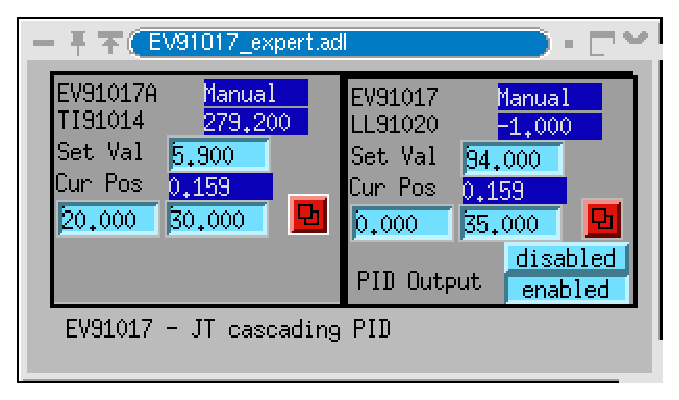
\includegraphics[width=3in]{beamline/ev91017_cascade.eps}
\caption{PID MEDM Screen - EV91017 Cascade Loop}
\label{fig:ev17c}
\end{latexonly}
%----------------------------
\begin{htmlonly}
\htmlimage{scale=1.0}
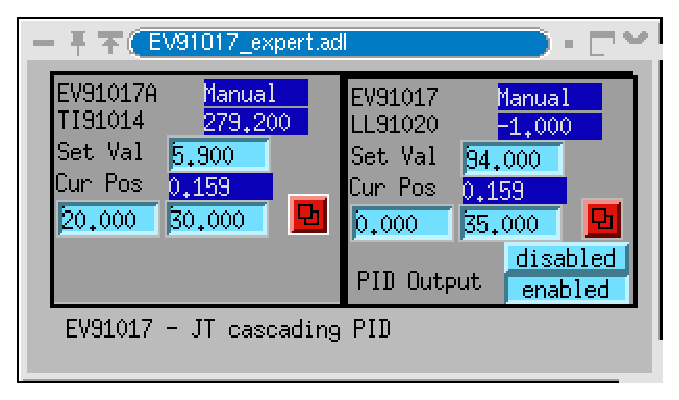
\includegraphics{beamline/ev91017_cascade.eps}
\caption{PID MEDM Screen - EV91017 Cascade Loop}
\label{fig:ev17c}
\end{htmlonly}
\end{figure}


\begin{figure}[h!]
\begin{latexonly}
\centering
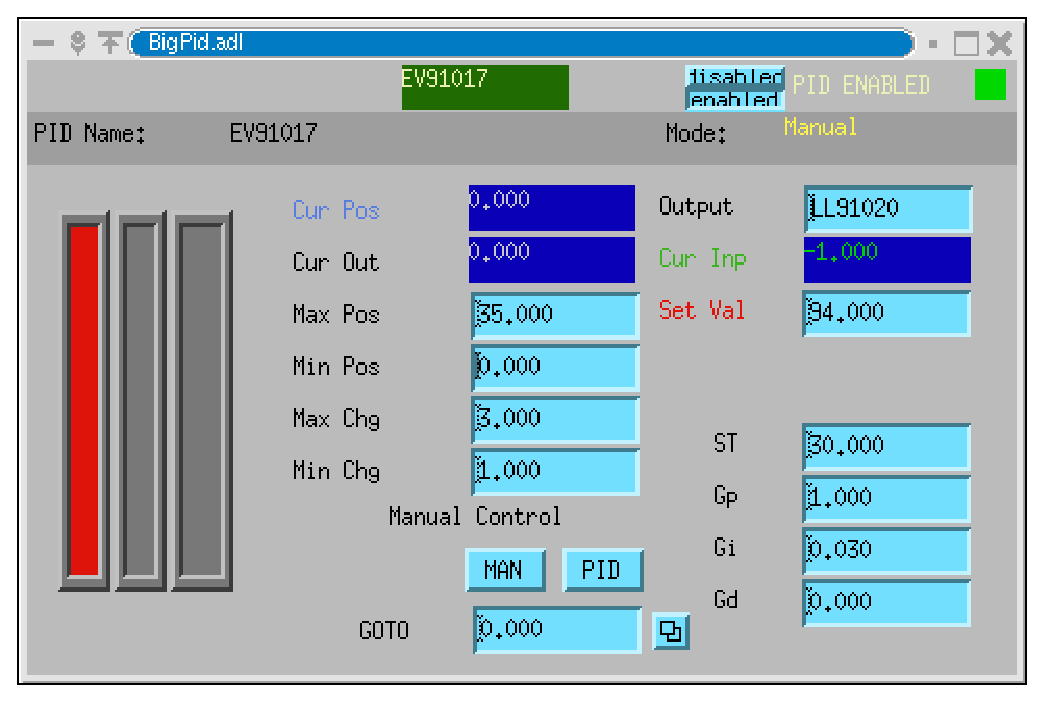
\includegraphics[width=3in]{beamline/ev91017.eps}
\caption{PID MEDM Screen - EV91017 Liquid Level Control}
\label{fig:ev17llc}
\end{latexonly}
%----------------------------
\begin{htmlonly}
\htmlimage{scale=1.0}
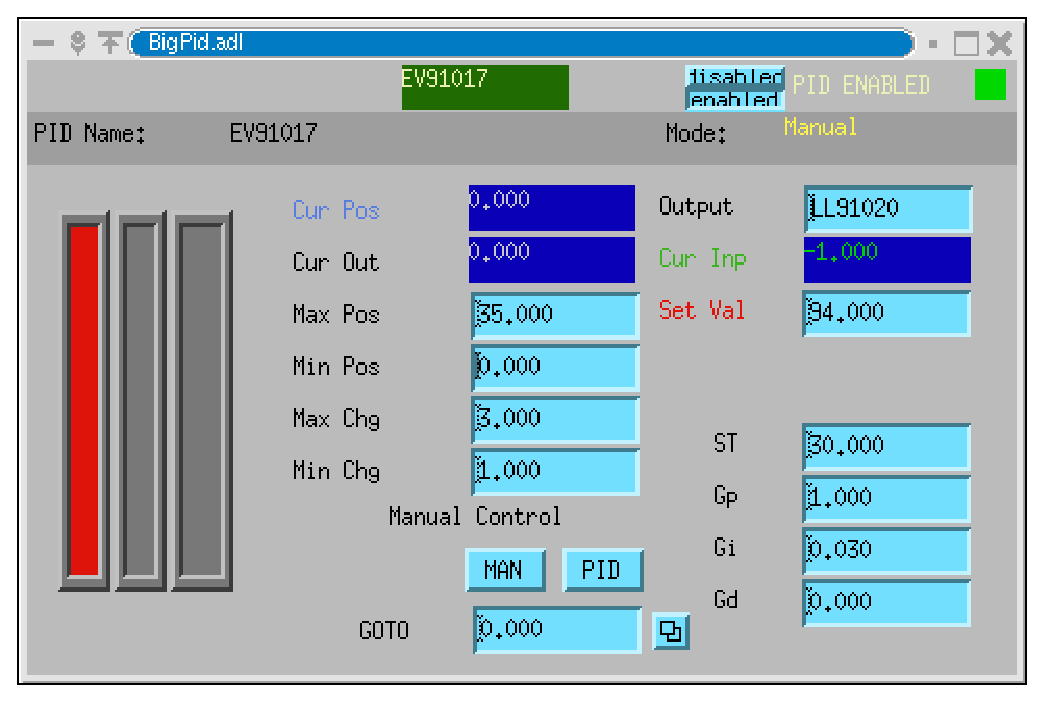
\includegraphics{beamline/ev91017.eps}
\caption{PID MEDM Screen - EV91017 Liquid Level Control}
\label{fig:ev17llc}
\end{htmlonly}
\end{figure}


\begin{figure}[h!]
\begin{latexonly}
\centering
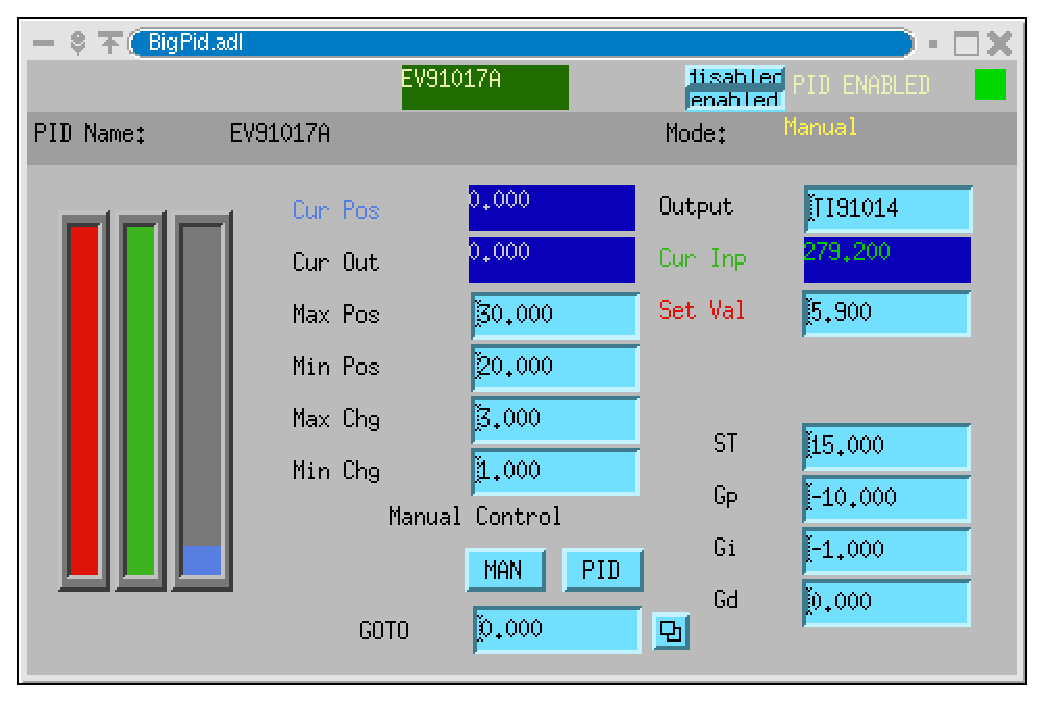
\includegraphics[width=3in]{beamline/ev91017a.eps}
\caption{PID MEDM Screen - EV91017 Helium Supply Temperature Control}
\label{fig:ev17stc}
\end{latexonly}
%----------------------------
\begin{htmlonly}
\htmlimage{scale=1.0}
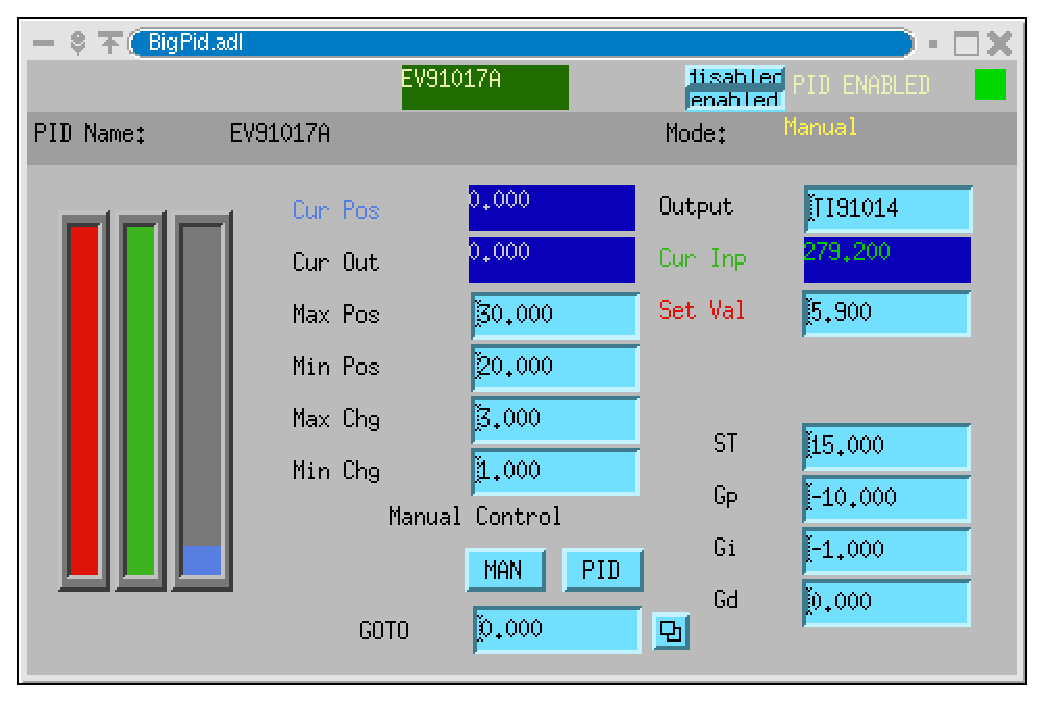
\includegraphics{beamline/ev91017a.eps}
\caption{PID MEDM Screen - EV91017 Helium Supply Temperature Control}
\label{fig:ev17stc}
\end{htmlonly}
\end{figure}




\subparagraph{Detector HV}
The HV of all detectors is controlled from the SOS HV
GUI. Nominal settings for the PMT's are given in Table~\ref{tab:mol_hv}.
If necessary, the M\o ller High Voltages can be controlled from the front panel
of the CAEN mainframe from which they are powered. This mainframe is the only
one in relay rack CHC15.
\begin{table}
\begin{center}
\caption{Nominal M\o ller Detector High Voltages and CAEN Power Supply Assignments\label{tab:mol_hv}}
\vspace{\baselineskip}
\begin{tabular}{|l|c|c|c|c|}
\hline
{}         & {}   & {}    & {}    & {}    \\
Detector   & Left & Left  & Right & Right \\
           & HV   & CAEN$\#$ & HV    & CAEN$\#$ \\
{}         & {}   & {}    & {}    & {}    \\ \hline
Pb Glass   & 1220* & 38   & 1310* & 39    \\
Hodo 01    & 1200  & 00   & 1220  & 05    \\
Hodo 02    & 1220  & 01   & 1190  & 06    \\
Hodo 03    & 1150  & 02   & 1120  & 07    \\
Hodo 04    & 1190  & 03   & 1100  & 08    \\
Hodo 05    & 1100  & 04   & 1120  & 09    \\
Hodo 06    & 1120  & 10   & 1200  & 15    \\
Hodo 07    & 1150  & 11   & 1100  & 16    \\
Hodo 08    & 1080  & 12   & 1270  & 17    \\
Hodo 09    & 1230  & 13   & 1100  & 18    \\
Hodo 10    & 1100  & 14   & 1180  & 19    \\
Hodo 11    & 1250  & 20   & 1150  & 25    \\
Hodo 12    & 1230  & 21   & 1200  & 26    \\
Hodo 13    & 1160  & 22   & 1150  & 27    \\
Hodo 14    & 1200  & 23   & 1180  & 28    \\
Hodo 15    & 1220  & 24   & 1170  & 29    \\
Hodo 16    & 1200  & 30   & 1150  & 35    \\
\hline
\end{tabular}
\end{center}
\end{table}
*{\it Note: The lead-glass voltages are beam energy dependent.}

\subparagraph{M\o ller IOCs Reference}

There are two IOCs which support the polarimeter devices. One
(iochc10 or {\it vmec10}) is on the Hall~C network and under the
control of Hall~C staff. It manages the superconducting solenoid
power supply and cryogenics system as well as the M\o ller target and
collimators. The other IOC (iochc11) is {\tt owned} by MCC. It
operates the two M\o ller quadrupoles. Software running on both
IOCs is maintained by the accelerator software group.

M\o ller quadrupoles Q1 and Q2 are controlled by the same IOC.
The power supply for Q2 communicates over GPIB. This requires a 
CPU board MV167 with an industry pack (IP)
for GPIB interface together with a HiDEOS board MV162 since EPICS
does not support GPIB directly. The CPU is called iochc11 (it had
been known as vmec11 prior to September 2001) and
is located in the right-hand half of a split backplane VME crate 
downstairs in the hall behind the green
shielding blocks. The EPICS drivers are located on the opsrv cluster.
The boot ROM looks as follows:

\begin{verbatim}
boot device          : ei 
processor number     : 0 
host name            : opsrv 
file name            : /cs/op/iocs/iochc11/vx/vxWorks 
inet on ethernet (e) : 129.57.242.11:fffffc00 
inet on backplane (b): 
host inet (h)        : 129.57.236.50 
gateway inet (g)     : 129.57.240.1 
user (u)             : vxwrks 
ftp password (pw) (blank = use rsh): 
flags (f)            : 0x0 
target name (tn)     : iochc11
startup script (s)   : /cs/op/iocs/iochc11/startup 
other (o)            : 
\end{verbatim}


The M\o ller target, collimators, solenoid power supply, and
solenoid cryogenics controls are all handled by vmec10 (also
known as iochc10) which resides in the left-hand side of the
same split backplane VME crate. Its boot ROM looks like:

\begin{verbatim}
boot device          : ei 
processor number     : 0 
host name            : opsrv 
file name            : /cs/op/iocs/iochc10/vx/vxWorks 
inet on ethernet (e) : 129.57.168.110:fffffc00 
inet on backplane (b): 
host inet (h)        : 129.57.236.50 
gateway inet (g)     : 129.57.168.1 
user (u)             : vxwrks 
ftp password (pw) (blank = use rsh): 
flags (f)            : 0x0 
target name (tn)     : iochc10 
startup script (s)   : /cs/op/iocs/iochc10/startup 
other (o)            : 
\end{verbatim}




%
\paragraph{Data acquisition}
The data acquisition reads out three Struck scaler modules at each
(possible) helicity transition. Scalers '1' and '2' are gated for '+'
and '-' helicity intervals as defined by the signal coming from
MCC. (For experiments using delayed helicity reporting the active
scaler will still be determined by the MCC signal, but this signal
does not necessarily indicate the instantaneous helicity state. The
actual state must be determined at analysis time.) Scaler '3' is gated
'on' during all helicity intervals, and should normally count the sum
of scalers '1' and '2'.

The CAMAC Crate is read out
on an prescaled event by event basis reading one ADC and one TDC
module and two dual port memories. The ADC and TDC provide diagnostic
information about the lead glass shower counters and the
M\o ller coincidence timing. The memories provide horizontal 
positioning information about the two M\o ller electrons in front
of the shower counters. This information is used to optimize
the quadrupole settings in order to center the 90$^{\circ}$ CM
M\o ller electrons on the lead glass. \\ \\
Data is taken using CODA2.1 running on cdaqs1. The run type
is Moller21 and can be started from the same location as the
main experiment.

\paragraph{M\o ller Beam line tuning}

A thorough step-by-step procedure for tuning the beam through the
polarimeter has been worked out with the MCC operations group. Only
MCC operators may modify the settings of the two M\o ller quadrupoles.
The procedure is available for your reference at
\htmladdnormallink{http://opsntsrv.acc.jlab.org/ops\_docs/online\_document\_files/MCC\_online\_files/HallC\_moller\_pol\_measurement\_proc.pdf}{http://opsntsrv.acc.jlab.org/ops_docs/online_document_files/MCC_online_files/HallC_moller_pol_measurement_proc.pdf}. In addition, there is a companion 
document for Hall-C operators to follow. It is available in print form in
the counting room, or on the web at 
\htmladdnormallink{Hall-C Moller Step-by-Step Guide}{http://www.jlab.org/Hall-C/document/manuals.html}.

The following is simply a coarse outline of the steps to be followed.
For actually tuning up the beamline and turning on the polarimeter, you {\bf must}
refer to the separate documents mentioned above. The tuneup procedure should take no
more than about 20 minutes if the beam is already tuned to Hall~C.
The time required to ramp up the superconducting solenoid is about 10 minutes.
\begin{enumerate}
        \item With all M\o ller magnets off MCC will
           center  the beam through the BPMs at 3C17  in both
           horizontal  and vertical  directions. 

        \item MCC will then turn on Q1, re-center the beam, then turn
	on Q2 and re-center the beam again. The required quad currents
	must be supplied by Hall~C.  (The M\o ller expert should have
	posted them in the logbook.)

        \item MCC will request that the Hall shift crew ramp up the
	M\o ller solenoid. We normally run it at 3~Tesla.

        \item With the solenoid and the two quadrupoles Q1 and Q2 on
              at nominal current, MCC will once again center the beam
              through the polarimeter and into the hall.

	\item If it is desired to take M\o ller measurements at beam currents
	      higher than $\approx$ 2 $\mu$ A it will be necessary to energize
	      the M\o ller raster system. See the documentation in
              \begin{verbatim} ~cdaq/documents/beamline/Moller_Raster_Manual.txt \end{verbatim}
\end{enumerate}


\chapter{Targets}

\section{The Hall~C Scattering Chamber}

The scattering chamber consists of a large central band made from a single
forged ring of 6061-T6 Al. This ring has an inner diameter of
48.5 inches and a  2.5 inch wall (0D = 53.5 inch). The ring has
cutouts consistent with the vertical angular acceptances and the
full angular ranges of the two Hall~C spectrometers. In addition,
the cutout for the SOS has been made to accommodate 20 degrees
of out of plane movement. There are also openings through which the beam
will enter and exit, a pumping port, several ports for viewing, and
some ports for as yet unspecified purposes.

There are two shells which are attached to the outside of the central
band. These are cylindrical sections which have an inner diameter
equal to the outer diameter of the scattering chamber. These shells
are designed to carry sliding vacuum seals so that the scattering
chamber vacuum can be directly coupled to that of the two spectrometers.
The SOS shell is mounted on a set of ``sliders" and can be moved
up and down by a series of linear actuators in order to accommodate the
out of plane motion of the spectrometer.

In the early stages of operation these shells are replaced by
clamps which hold thin fixed metal vacuum windows.

The opening for the SOS is five inches tall. The metal window is
5052-H39 aluminum 0.008 inches thick. This is the same foil that was used to
cover the five inch tall window on the temporary Hall~C scattering chamber
(The SLAC chamber). This is the same material that was used by SLAC when
the chamber was in use there.
The opening for the HMS
is eight inches tall. This will be spanned by a window of
5052-H34 aluminum 0.016 inches thick. The tank has been pumped down with
{\bf both openings covered by 0.008 inch thick 5052-H39 }
and vacuum cycled several
times. The crinkling pattern was examined and the inter crinkle spacing
was used as input for stress calculations. In this approximation the
total window is treated as a collection of smaller windows each of which
has a height equal to that of the full opening and a width given by the average
inter crinkle spacing. These calculations indicate that the windows
proposed above (0.008 inch for SOS and 0.016 inch for HMS) have at least
a factor of two safety margin.

These windows have been tested to failure with over pressure from the
outside.  The average failure pressure exceeded 40 psid and thus they
have a safety margin of over 2.5.  

There are also top and bottom plates which complete the main body of the
scattering chamber.

The bottom plate allows the chamber to be mounted to the
solid shaft which forms the pivot axis for the two spectrometers.


The top plate has a number of openings. The largest of these allows
the cryotarget plumbing and lifting mechanisms into the vacuum and is sealed by
a large diameter bellows. There is also a three inch diameter tube through
which the solid targets are inserted.
The other three openings are capped by eight inch diameter aluminum
conflats and currently have no specified function.

The beam entry and exit tubes are vacuum coupled to the scattering chamber with
metal seals. The beam exit tube terminates in a 0.015 inch thick beryllium foil.
This window should be regularly inspected for signs of deterioration.

%All questions about the scattering chamber or its vacuum windows should
%be referred to J. Mitchell -x7851.

\section{The Solid Target Ladder}

The scattering chamber has two target ladders associated with it,
a cryogenic target ladder and a solid target ladder. To change
from the cryogenic target ladder to the solid target ladder, one has
to:

\begin{itemize}
\item{Move the cryogenic target ladder to its home position.}
\item{Rotate the cryogenic target ladder over 90 degrees. This removes
the cryotargets from the beam line, and moves them out of the spectrometer
acceptances.}
\item{Insert the solid target ladder and select the appropriate target.}
\end{itemize}

\noindent To install the cryogenic target ladder again, one has to reverse the
process:

\begin{itemize}
\item{Move the solid target ladder to its home position (completely out
of the way).}
\item{Rotate the cryogenic target ladder back into place (-90 degree
rotation).}
\item{Select the appropriate target.}
\end{itemize}

We have four different solid target systems currently in use in the
Hall C Scattering Chamber.  There is a solid target attached directly
to the cryotarget and three versions of the independent solid target
ladder system.

The solid target that is attached to the bottom of the cryotarget is
often referred to as the optic target.  This target is a system of
aluminum and carbon foils arranged at different locations and heights
relative to the beam.  The foils provide cryotarget window
calibration and loop target spectrometer optics calibration.  The
various targets are brought into the beam by simply closing the
vertical height of the cryotarget stand and a ``scan'' can be made
that spans the length of the cryotarget in discrete steps on window
convection data taken.  This system replaced the earlier ``slanted
target'' system.

The independent solid target system has three different ladders which
mount interchangeably to the same mechanism.  This mechanism
provides for a telescopic guidance system with good accuracy
and stability as well as vertical, and rotary control.  The rotary mechanism also
has an integral rotary water feed thru for high power solid target
runnings. 

The three solid target ladders use identically sized interchangeable
variable thickness solid targets.  They use a common target mounting
system.  The three ladders currently available are:

\begin{itemize}
\item{Un-cooled target ladder with a standard solid target position.
This is for 0-30 $\mu$A rastered beams for materials with good
conductivity and high melting points.}
\item{Water cooled target ladder with 6 standard solid target
positions.  This is for 0-100 $\mu$A beams that are rastered.  These
can handle any material.}
\item{Combination water cooled solid and water target.  This target
has, in addition to 5 solid target positions, a new water cell.
The water cell is 1 cm thick and has entrance and exit windows of 0.1
mm (~.005 in) aluminum.  The water cell is all machined and welded to
the bottom of the solid target ladder.}
\end{itemize}

In some cases the solid targets will be cooled with water to prevent
destruction of the targets by a high current beam. If this is the case
make sure that the
cooling water is indeed flowing before the experiment starts.
{\sl Failure to do so may cause loss of the targets}. Often we
do not have to use water cooling. This is the case when we are
rastering the beam, or are dealing with solid target
materials with excellent thermal conductivities (like pyrollytic
graphite or ceramic BeO) and currents less than or equal to 30 $\mu$A.

In all cases, as we may use these targets in conjunction with a high
energy, high current beam a large level of radiation may be induced
in these targets.

The main safety issue concerning the non-special targets is that
they will be radioactive (``hot") after they have been
exposed to the JLab beam for an experiment.
Targets may not be removed from the target chamber ot transported from the Hall without 
concurrence by the RCG. An SRWP specifies the requirements for target removal and/or 
transport. Targets which have been surveyed and released by the RCG will be stored in a 
second fire safety cabinet which has been designated for target storage and is located in 
the hall.

Since the targets may be water cooled, we will induce a slight
radioactive level in the cooling water. However, the cooling water
system is a closed loop, and calculations performed by the Radiation
Safety group indicate that the radioactive level induced is minimal.
Also, to ensure that the cooling water is indeed a contained system
and can not leak out to the environment, the pumping system causing
the water to flow is placed in a tray.

\subsection{Special Targets}

Some of the solid targets require special attention. In some cases
mishandling of the targets is relatively innocent, like in the case
of the natural {\bf Calcium} target. This material, when exposed to air,
will oxidize, resulting in a large oxygen content in the target.
Store natural Calcium always in an argon-filled or vacuum closed
case, or in an oil solution. Calcium can be handled in air for a limited
amount of time (a few hours) if handled with a layer of oil.

Other special targets may pose a safety concern. At this
moment the only twos special target materials we own are ceramic
{\bf Beryllium-Oxide (BeO)} and {\bf Beryllium (Be)}.
In solid form, BeO is completely safe under normal conditions of use.
The product can be safely handled with bare hands.
However, in powder form all Beryllia is {\bf toxic} when airborne.
{\bf Overexposure to airborne Beryllium particulate may cause a
serious lung disease called Chronic Berylliosis. Beryllium has also
been listed as a potential cancer hazard. Furthermore exposure to
Beryllium may aggravate medical conditions related to airway systems
(such as asthma, chronic bronchitis, etc.).}
Since beryllia are mainly dangerous in powdered form, do not machine,
break, or scratch these products. Machining of the Beryllia can only
be performed after consulting the EH\&S staff.
It is good practice to wash your
hands after handling the ceramic BeO. If handling the pure Beryllium
target wear gloves and an air filter mask.

\subsection{Storage}

The targets {\bf must} be stored in a safe, locked place tagged with the
appropriate radiation signs. At this moment we use a small yellow
fire safety cabinet for this purpose. The cabinet is stored in the
little backroom of the Hall~C counting house. The key of the target
storage cabinet can be found in the Hall~C key box, hanging on the
wall next to the Hall~C counting house entrance.
Targets may not be removed from the target chamber or transported from the hall without 
concurrence by the RCG.  An SRWP in the counting house specifies the requirements for 
target removal and/or transport.  Targets which have been surveyed and released by the 
RCG will be stored in a second fire safety cabinet placed downstairs in Hall~C,
that has been designated for target storage.

Since we will typically have
Be and/or BeO targets stored in this cabinet too, also signs indicating
the presence of Beryllium materials (``Beryllium Storage")
are tagged to this cabinet. The Material
Safety Data Sheets for Beryllia are included in the storage cabinet.


\section{The Cryogenic Target System}

Much of the physics program at JLab requires the use of cryogenic targets
filled with hydrogen, deuterium or helium isotopes. The Hall~C cryogenic
system contains three separate loops in order to allow for rapid changes
of target fluid.  This system will be extensively discussed in
another section.  Here, we only summarize some main features.

A target loop is a circulating system of target gas and consists of the following
elements:

\subsection{Target Circulation Fan} This is some sort of device to keep
the target fluid circulating through the system. In the Hall~C cryogenic
targets this function is performed by a two stage axial flow fan which is
immersed in the target fluid. This is a small AC motor with fan blades attached
on both shafts of the rotor. The blades in our case are simple Archimedes
screws with a diameter of 2.8 inches. The motors where extracted from Globe
VAX-3-FC Blowers, part $\#$ 19A798. The factory installed
bearings were then replaced with bearings suitable for cryogenic service
(Barden, Bartemp-no lube SR4SSTB5). The fans are powered asynchronously
with three phase AC power from a variac and since the stators are wound with
two poles the maximum rotation speed is 3600 rpm.
\subsection{Target Cells} This is the thin walled vessel in the circulation loop
where the electron beam interacts with the target fluid. Two types
of target cells will be employed in Hall~C. These are the ``beer can" cells
and the vertical flow cells. The vertical flow cells are also referred
to as ``tuna can" or ``sink trap" cells.
The beer can cells are constructed from Coors beer cans (3004 series aluminum)
and come in two standard lengths, 4 cm and 15 cm.
The vertical flow cells are 4 cm in length and are constructed from 7050
series aluminum.
\subsection{Heat Exchangers} This is where the heat that is deposited in the target
fluid by interaction with the electron beam is removed. The target fluid is
circulated on one side of the heat exchanger and cold helium
from a refrigerator is circulated through the other side of the heat exchanger.
The cryogens for the Hall~C target will be supplied from the End Station
Refrigerator (ESR).

A new feature in 1999 is the conversion of the cryotarget cooling from
the previous series/parallel flow to a pure parallel flow cooling
system.  This was done to make control of the three cryotarget loops
simpler, truly independent, and truly interchangeable.  The use of
LN$\_2$ as a precooler was elected in favor of directing a small
amount of the 20K exhaust helium.  

\subsection{Heaters} The temperature of the target can be regulated by powering
a heater immersed in the target fluid.

\subsection{Other Features of the Cryotarget System}  In addition to the above components which make up the loop a cryogenic target
needs a gas handling system and instrumentation. The gas handling system
enables the operator to fill, empty and perform other manipulations of the
target while the instrumentation is needed in order to verify the target's
status, temperature, pressure, etc. The temperature is particularly critical
in that it is the dominate parameter that is correlated to target density.

A system of several targets also needs a motion mechanism so that the desired
target can be inserted in the beam. The Hall~C target accomplishes this by
means of a three rail system, two ball screws and a guide bearing.
The ball screws are driven by two AC motors each of which has a resolver and
a 50 to 1 gear reducer. The resolver output of one of the motors is used
to track the position with one of the motor controllers acting as a master
while the second controller is slaved to the master.

All the instrumentation and control of the target system is implemented
via the EPICS system (this is the same control system used by the main
machine).

%Questions concerning the cryogenic targets should be referred to J.H. Mitchell
%at extension 7851.

%\vfil
%\eject

\section{Bremsstrahlung Radiator}

The Bremsstrahlung radiator consists of a target ladder with
several thicknesses of natural Cu of size 1.5" times 0.75".
Typical radiator thicknesses are 2\%, 4\%, and 6\%, all in
radiation lengths. The Bremsstrahlung radiator is the last element
in the Hall~C beamline before the scattering chamber, at a distance
of about 1.2 meter from the physics targets.

The target ladder can be moved in and out of the beam by use of
a stepping motor. Targets are cooled with water to prevent destruction
of the targets by a high current beam.
Because we may use these radiator targets in conjunction with a high
energy, high current beam we may produce a large amount of background
in the radiator, and radiation in the parts around the radiator.
For this reason the Bremsstrahlung radiator will be enclosed by a lead
shield.

The only safety issue concerning the Bremsstrahlung radiator is that of
induced radioactivity in
the Cu targets, or more seriously, in the water used for cooling the targets.
 The water cooling system is a closed loop. The heart of the system is
a portable welding torch water cooler. This device is kept in a tray
which is intended to provide secondary containment in case of a leak.
 The cooling system must not be breached or drained without concurrence from the RCG.  
Accidental breach or spill constitutes a radiation contamination hazard.  A spill control kit, 
capable of containing a system leak or spill, is staged in the hall next to the cooling system 
tray.  The cooling system is located    .

The Cu targets will certainly be activated in the course of an experiment.
Therefore, only remove
the Cu target, the target ladder, the shielding around the radiator,
and/or the whole radiator system in the presence of a Radcon technician.

\paragraph{Radiator Control}

In one of the xterm windows, type the following:

\begin{verbatim}
	cd ~cdaq/bin
	Radcontrol
\end{verbatim}

and use the menu session to control the motion of the
Bremsstrahlung radiator.

The source code can be found in:

\begin{verbatim}
	cd ~cdaq/bin/Rad_source
\end{verbatim}

Do not change the source code without consulting
%Dave Meekins or
one of the JLab Hall~C staff.

\chapter{The Hall~C Spectrometers}

%\section{Introduction}

	The two magnetic spectrometers in Hall~C are the principal instruments
available for use in electron scattering experiments. In the following three
Sections we discuss the safe operation of these two spectrometers,
the High Momentum Spectrometer, or HMS,
and the Short Orbit Spectrometer, or SOS. The spectrometers are
discussed as a series of subsystems.

Both spectrometers are composed of a magnet system, consisting of both
quadrupole and dipole magnets. The HMS has a triplet of superconducting
quadrupoles, while the SOS has only one resistive quadrupole magnet.
The primary purpose of the quadrupole magnets is to increase the flux of
charged particles entering the dipole magnet and to focus the orbits of the
charged particles into the detector plane.
The HMS has one superconducting dipole magnet following the quadrupole triplet,
and the SOS has two resistive dipole magnets. The primary purpose of these
dipole magnets is to deflect charged particles such that they can be momentum
analyzed.
Each spectrometer has a rotatable support structure, called the
carriage, which supports the magnets.

In addition, there is a separate
structure which contains the particle detector packages the shield house.

The HMS shield house is attached to the carriage via a ``push bar" on the ``pasta
fork".  The ``pasta fork" is the name given to the steel piece that protrudes
from the back of the carriage. The detector frame is supported on the
``pasta fork." This insures that the detectors do not move relative
to the magnetic elements.

The detector package must perform at least two functions, tracking and
particle identification (PID). A particle traversing the detector stack
encounters two sets of drift chambers with six planes of sense
wires in each chamber. From the chamber information both positions
and angles in the dispersive and transverse directions can be determined.
The information from these chambers is the principal input
of the tracking algorithms.

The chambers are followed by two planes of hodoscopes designated S1X and S1Y.
These plastic scintillator arrays provide the timing reference for the
drift chambers, are used in trigger formation, and in combination
with a second hodoscope pair, provide time-of-flight particle identification.
These scintillators can also be used to perform crude tracking.

The next element encountered by a particle is a gas threshold Cerenkov detector.
This is used for particle identification. In the SOS spectrometer, this
gas threshold Cerenkov detector can be replaced by an Aerogel detector,
with a similar function.

The second hodoscope pair, S2X and S2Y, is located directly behind the
gas Cerenkov. Their function is essentially the same as that of S1X and S1Y.
In the SOS spectrometer, an option exists to have this hodoscope pair
be preceded by a third chamber to improve tracking.

The final element in the detector stack is the lead glass shower calorimeter.
This is used for energy determination and PID.
	
To reduce the resolution degrading effects of multiple scattering, the entire
interior of the spectrometer from the pivot to the detector hut is a vacuum
vessel. The ends of this evacuated
volume are capped by relatively thin vacuum windows.

The aforementioned subsystems will be discussed in more detail in the next three
sections. The remainder of this section will describe some features common to
the two spectrometers, then the following major sections will be devoted to the specifics 
of the HMS, and the SOS, respectively.

\subsection{Features Common to Both Spectrometers}

\subsubsection{Vacuum Windows}

\paragraph{Overview}

Because multiple scattering degrades the performance of a spectrometer, it is
important that the spectrometer volume be evacuated and that the vacuum
entrance and exit windows
be as low mass as possible. However,
catastrophic window failure would generate a significant shock wave as air
rushed to fill the vacuum volume. It would also cause a loud noise which
could cause hearing damage to anyone in the immediate vicinity.
The material chosen for the vacuum windows, then, must be both light enough
to have a minimum effect on the beam and
strong enough to operate reliably and safely.

To achieve the above goals,
composite Mylar/Kevlar vacuum windows have been constructed for the
Hall~C spectrometers. The density of the Kevlar used
is $\approx 0.75$ gm/cm$^3$ with a radiation
length of $55.2$ cm \cite{rdup1}. The radiation length
of Mylar is $28.7$ cm. The Kevlar has a tensile strength of 900 lbs/inch.

The HMS spectrometer vacuum can has a volume
of approximately $6$ m$^3$, representing a stored energy of $6 \times 10^5$
Joules. A drawing of the exit flange to which the vacuum
window is attached is shown in Figure~\ref{fig:hms_flange}.  It is a
circle with a center-to-center bolt hole diameter of $40$ inches
and a $38$ inch diameter vacuum opening. This is the largest vacuum window
required for Hall~C.
Under vacuum, this window must support 16,785
lbs (74,425 N). It is located in the HMS detector hut. The HMS
entrance window is located near the pivot and has a center-to-center
bolt hole diameter of $10.5$ inches.

\begin{figure}
\includegraphics[width=6in]{spectrometers/figHMSflange.eps}
\caption{The HMS exit flange and the 8" vacuum spool piece. \label{fig:hms_flange}}
\end{figure}

The SOS spectrometer vacuum can has a volume of approximately $2$ m$^3$,
representing a stored energy of $2 \times 10^5$ Joules. The entrance
window (near the pivot) is round and has a diameter of $9$ inches.
The SOS exit window is the second largest window in Hall~C. This
window is located in the SOS detector hut. It is rectangular.
The opening has a length of $40.5$ inches and a width of $6.5$ inches.
The SOS exit
window must support a load of $3,896$ lbs ($17,275$ N) under vacuum.

{\bf One of the responsible personnel must be present for
any work directly affecting a Hall~C vacuum window}.

\paragraph{Design and Placement of HMS Large Window}

After extensive testing of the above design
and of other similar designs and fabrics (Spectra, Kevlar/Nylon fabric),
we chose to have a new
material custom laminated for our purposes. The new window material is
composed of 0.015 inch ballistic Kevlar 29 style 713 (31x 31 count,
plain weave)
with 0.004 inch Mylar on
one side
and 0.001 inch thick Mylar on the other. Bolt holes are cut into the material
(using a custom made cutting tool) and it is then directly
mounted on a ring flange using standard O-ring vacuum
seal technique.  This material and
method have
been used successfully on both Hall~C spectrometers, holding a vacuum of
$\approx 10^{-4}$ Torr. It is necessary to have a large number of bolt holes in the flange ring
for clamping strength.

Figures~\ref{fig:hms_window} shows the
window and ring flanges as mounted on the spectrometer. The thick
line represents the composite window. There are O-ring grooves on both the
ring flange for the window mount and on the spectrometer exit flange.
The ring flanges are rounded so as not to cut into the window fabric as
it bows under pressure.
For more detail on the window mounting, see
the section entitled ``Vacuum Window Installation Procedure", below.

\begin{figure}
\includegraphics[width=6in]{spectrometers/figHMSwindow.eps}
\caption{The HMS vacuum window and ring flanges. \label{fig:hms_window}}
\end{figure}

Figure~\ref{fig:hms_window2} shows the window as placed in the HMS spectrometer
detector hut.
\begin{figure}
\includegraphics[width=6in]{spectrometers/figHMShut.eps}
\caption{The HMS vacuum window in the HMS spectrometer hut. 
\label{fig:hms_window2}}
\end{figure}

The window (in its ring flanges) is mounted at the end of the $8$ inch
vacuum exit extension piece. The next element is an aluminum shutter which
must be lowered to cover the Mylar/Kevlar window whenever it is under
vacuum and personnel are working in the detector hut. The shutter
control panel is just outside the shielding house door, and an
indicator light signals whether the shutter is in or out.  

\paragraph{Other Windows}

The HMS spectrometer vacuum entrance is a $10.5$ inch (bolt circle) round
window. Presently, the entrance window
is made of the same laminate as the exit window. The
procedure for installation (see below) is also the same.
It is
also allowable to employ thinner Kevlar/Mylar
material for the HMS entrance window and for
the SOS spectrometer windows; a similar laminate as used in the
larger windows has been tested and utilized.  The thinner material is
composed of 0.0045'' Kevlar sandwiched between 2 sheets of 0.002'' Mylar.

The SOS spectrometer windows are currently made of the same composite fabric
as the HMS windows. The SOS exit window is rectangular, with a $6.5$ inch
by $39.5$ inch opening.
The window is cut out and installed with an O-ring as with the HMS
windows (see Figure~\ref{fig:hms_window}).
Because the maximum
loads under vacuum on the SOS windows (and HMS entrance window)
are much smaller than that on the HMS exit window,
there is
no aluminum shutter in the SOS spectrometer.

\begin{figure}
\includegraphics[width=6in]{spectrometers/figSOSwindow.eps}
\caption{The SOS exit window and the vacuum test tank. \label{fig:sos_window}}
\end{figure}

\paragraph{Window Material Testing}

Standard models used in predicting vacuum
window performance do not predict the actual performance of Kevlar laminate
fabrics accurately \cite{rbrook1,rllnl2}. Therefore, extensive tests of the
Mylar/Kevlar composite windows have been done and more are planned.
A summary of pressure
tests on windows composed of the custom laminated
fabric currently used in construction of all Hall~C vacuum windows is
given in Tables~\ref{tab:win_tst1} and \ref{tab:win_tst2}, below. Both vacuum and hydrostatic test 
tanks
are available for the HMS circular windows and for the SOS rectangular
window. Figure~\ref{fig:sos_window} shows a picture of the SOS vacuum
test tank.  The large round
HMS vacuum test tank uses the $8$ inch vacuum extension piece shown
earlier in Figure~\ref{fig:hms_window} (but removed from the spectrometer) with a $1.5$
inch thick aluminum blanking flange. For hydrostatic testing, windows (both
round and rectangular) are mounted directly on
blanking flanges with appropriate water fittings installed.

\begin{table}
\includegraphics[height=7.5in]{spectrometers/vacuum.ps}
\caption{Tests on the Hall~C Vacuum Windows (1 of 2) \label{tab:win_tst1}} 
\end{table}
\clearpage

\begin{table}
\includegraphics[height=7.5in]{spectrometers/vacuumc.ps}
\caption{Tests on the Hall~C Vacuum Windows (2 of 2) \label{tab:win_tst2}}
\end{table}
\clearpage

The tests show that the large HMS exit window does not begin to leak until
the pressure on it reaches over $3$ atmospheres. The small HMS window
did not begin to leak until over $14$ atmospheres of pressure was applied.
This is consistent with the load being transferred to
the outer circumference, the circumference of the small circle being four
times smaller than that of the large circle. The large rectangular SOS windows
began to leak at around 10 atmospheres. It may be possible to construct thinner
SOS vacuum windows for improved spectrometer resolution if required.

In addition to determining the absolute failure
pressure of the windows, a major goal of the testing effort was to
observe the failure modes of the
window material and flange design. The large windows failed by
ripping around the opening perimeter. The flange ring was then
rounded more and
a better result was obtained. It may be possible to further round the
flange if future tests indicate this to be necessary or advantageous.
The small windows failed by ripping out at the bolt holes.

Another question the tests in Table~\ref{tab:win_tst1} were designed to
answer was if
a biting aluminum clamping O-ring was necessary or advantageous. It was found
that windows with aluminum clamping rings failed at lower pressures than
windows without aluminum rings. The aluminum tended to tear the Mylar, allowing
leaking and uneven stress. The only window which delaminated had water between
the Mylar and Kevlar which leaked in through a tear in the
Mylar caused by the aluminum ring.

In conjunction with outlined full-size window testing, small samples
were subjected to stress and tensile analysis using strain gauge
instrumentation.  Through this work, it was found that the composite
window material maintained the Young's Modules of Kevlar, and had the
same ultinate failure load as Kevlar pieces of the same size.
Further, it was determined that the failure tears were along a
45$^{\circ}$ angle to the woven fibers, consistent with observations
of the rips in the destructively-tested full-size windows.  

In addition to the above testing efforts, two large round HMS exit windows
composed of the custom laminate material were ``knife" tested. The windows
were installed on the vacuum test tank and placed under vacuum. They were then
cut by a blade at the end of a long pole (so as to protect the personnel
testing the window from the results of a catastrophic failure). The window
did not rip any further than the cut and the
material did not delaminate. No evidence for catastrophic failure
was observed in either of these tests.

Although more long term reliability testing is necessary (see below),
results have so far been favorable.
Windows previously used on the HMS spectrometer are routinely hydro
tested to failure after biannual removeable and found to
hold up as well as freshly made windows (see, for example
Table~\ref{tab:win_tst1}).  Windows which have undergone multiple cycles fail at nearly the same pressure as uncycled
windows (see, for example, Table~\ref{tab:win_tst2}). A small round window did not fail after
being left pressurized for
a week at $65$ psi. (this test is not entered in the tables).
Entrance and exit windows composed of the Mylar/Kevlar laminate
material here described have held vacuum on the Hall C
spectrometer effectively and safely for over three years.


\paragraph{Vacuum Window Fabrication and Installation Procedure}

This procedure must be followed for installing any Hall~C spectrometer
vacuum window. One of the responsible personnel must be present during
all steps of fabrication and installation.
Although the procedure below is specifically for
the HMS large window, it is the same for the small HMS and for both SOS windows,
except as noted.
\begin{enumerate}
\item{Place window material, thin Mylar side down,
on a large flat, extremely clean, surface (such as
the marble table in EEL 126 after being washed).}

\item{Place window flange ring (also freshly cleaned) on top of material
and trace outer
circle (or rectangle for SOS) and bolt holes with transparency marking
pen.}

\item{Remove flange ring and cut out circle using Kevlar cutting 
shears.}

\item{Cut out bolt holes using appropriate (custom-made) drill press tool.
For the larger windows, this is a two person job as one is needed to hold the
material up so that it can't be nicked by the side of the drill press table
while the other concentrates on cutting the holes.}

\item{Clean the aluminum flange ring thoroughly and wipe with isopropyl
alcohol. For all but the HMS exit window, the flange ring and
window should be brought to the hall.  For the HMS exit window,
continue as outlined below from step 6 on.  For all other windows,
install flange ring and window unit to spectrometer vacuum flange
using standard O-ring vacuum seal practice (i.e. clean all surfaces
thoroughly with alcohol, apply vacuum grease, tighten in star pattern,
etc.)  All bolts should be torqued to 50 ft-lbs (40 ft-lbs for the
SOS exit window).  There must be a correctly tightened bolt in every
bolt hole.  Continue to step 17.}

\item{{\sl (HMS exit window)} Clean Viton O-ring with isopropyl alcohol and apply vacuum
grease as is standard for vacuum connections.}

\item{{\sl (HMS exit window)}Place Viton ring on HMS vacuum extension piece, composite
window over ring, and aluminum flange (clamping) ring over window.   Bolt together at four corners.}

\item{{\sl (HMS exit window)}Place and tighten bolts in a star pattern as appropriate for
standard O-ring vacuum seals.}

\item{{\sl (HMS exit window)}All bolts should be torqued to 50 ft-lbs (40 ft-lbs for the SOS
exit window).}

\item{{\sl (HMS exit window)}Using standard O-ring seal technique, mount other side of
vacuum extension piece on aluminum blanking flange.}

\item{{\sl (HMS exit window)}Using a transparency marker, trace the flange circle onto the
Mylar/Kevlar window.}

\item{{\sl (HMS exit window)}Begin vacuum pumping on extension
piece.} 

\item{{\sl (HMS exit window)}Note any creep of traced ring and window
deflection.  Check window for visual abnormalities or imperfections.}

\item{{\sl (HMS exit window)}Leave under vacuum for at least 1 hour.
Repeat step 13.}

\item{{\sl (HMS exit window)}Bring vacuum extension piece back to
atmospheric pressure and remove blanking flange.}

\item{{\sl (HMS exit window)}Being extremely careful not to touch the
Mylar/Kevlar window, install extension piece on HMS spectrometer in
hut using standard O-ring vacuum practice.}

\item{Clear detector hut and pivot area for initial pump down. Do not
allow entry for anyone other than the above named personnel to
these areas until a vacuum of at least 50 mTorr is achieved.}

\item{Begin vacuum pumping.}

\item{One of the above named personnel should check and note the
window deflections, recheck bolt torques, and generally look for
irregularities in the window deflections, before allowing
general entry to the detector
hut or pivot areas. That person should wear ear protection at all times while
near windows. Bolts should be retorqued if necessary.}

\item{Place a clearly visible tag near the vacuum window indicating
date of installation, estimated date of removal, and names and phone
numbers of contact personnel.}

\item{Recheck bolt torque, vacuum, and window deflection
again a couple of hours later (again, this should be done by
qualified personnel only, wearing hearing
protection). Retorque bolts if necessary.
If the window deflection has increased more than 3/4 inch, begin the entire
process again with a new window.}

\item{The windows should be changed as close to every 6 months as
reasonable given experiment run scheduling considerations. It is not
necessary to stop a run to change the windows, but they should be changed
as soon as possible thereafter.}

\end{enumerate}

%\paragraph{Safety Procedure for Working Near Vacuum Windows}

%Before entering the detector huts or pivot area, all personnel should check
%the spectrometer vacuum gauges. The HMS gauge is located under and near the Q3
%quadrupole. The SOS gauge hangs from the carriage beneath the quadrupole.
%Both gauges are monitored by video cameras and may be viewed
%in the counting house.
%If the spectrometers are under vacuum, the following procedure should be used.
%
%\begin{enumerate}
%\item{Before entering detector hut or pivot area, put on hearing
%protection. It is recommended that nobody should be
%closer than 3 feet from the windows without ear protection and that only
%those personnel who need to approach the windows be in their immediate
%vicinity.}
%
%\item{If entering HMS detector hut, close aluminum
%shutter over vacuum window before entering.}
%
%
%\item{If entering pivot area, check both spectrometer windows visually
%(from a distance greater than 3 feet if possible) for obvious wrinkles or
%discoloration. If any are observed, vacate area and
%contact one of the above named personnel. Never touch the vacuum 
%windows.}
%
%\item{Use careful judgement if it is necessary to work near the vacuum
%windows. Do not place objects so that they may fall on the windows, 
%etc.}
%
%\item{Do not work near the windows any longer than is absolutely
%necessary.}
%
%\item{Open aluminum
%HMS exit shutter only when all personnel have left the detector
%hut.}
%\end{enumerate}
%
%\paragraph{Vacuum Window Safety Summary}
%
%Catastrophic window failure would generate a significant shock wave as air
%rushed to fill the evacuated volume. It would make a loud noise which could
%damage the hearing of anyone standing close at hand at the time of failure.
%There are several indicators that something is wrong with the vacuum. If
%any of the following are observed, qualified personnel should be contacted
%and no one should approach the windows until one of those personnel have
%deemed it safe:
%
%
%
%\begin{enumerate}
%
%\item{Visual defects, particularly wrinkles, discoloration, or
%uneven fiber stress.}
%
%
%
%\item{Date of removal on tag near spectrometer window indicates
%a date near or after current date.}
%
%
%\item{Vacuum gauges indicating a loss of vacuum
%$\ge 1$ mTorr.}
%
%\item{HMS shutter malfunction (troubles opening or closing).}
%
%\item{The pen-traced ring drawn onto thae window perimeter moving away
%from the perimeter.}
%
%\item{Bolt torque not remaining at installed value
%(only qualified personnel should check for this).}
%
%\item{Deflection increasing above installed value
%(only qualified personnel should check for this).}
%\end{enumerate}
%



\section{The High Momentum Spectrometer (HMS) }

The HMS is composed of three superconducting quadrupole magnets,
Q1, Q2, and Q3, and one superconducting dipole magnet. The quadrupoles
were manufactured for JLab by {\em OXFORD} while the dipole was built for 
JLab by {\em ELIN}.
The quadrupole magnets are referred to as Q1, Q2, and Q3, where a particle first traverses 
Q1, then Q2 and Q3, and finally traverses the dipole magnet.

The magnet system is followed by a large concrete detector hut, in which all
detector elements reside. The main fraction of the detector elements have been
built by universities involved in the Hall~C physics program.

The HMS magnet system is the cornerstone of the Hall~C activities.
Many of the experiments approved in Hall~C center on physics at high
momentum transfers and other short-range phenomena, and rely on a spectrometer
able to momentum analyze charged particles up to very high momenta.
The design value for the maximum momentum accessible to the HMS magnet
system is 6 GeV/c, though in its initial phase the maximum momentum
has been limited to 4 GeV/c.


\subsection{Magnets and Power Supplies}

The HMS magnets are all
superconducting and hence their coils must be maintained at
cryogenic temperatures during operations. The LHe required by the magnets
is supplied by the End Station Refrigerator, ESR.

All the HMS magnets cryogenic services are supplied through the overhead
cryogenic lines. The distribution network begins at the distribution
box over the pivot. This box is connected to the rest of the network via the
flexible transfer lines over the pivot. The network is adjacent to
the upstairs catwalk of the HMS.

Cryogenic information about each magnet is available on the control screens
downstairs, one for each magnet. These are located on the first deck
of the shield house by the ``pasta fork" at the rear of the spectrometer.
Normally during run periods the control screens are sent upstairs to the
Hall~C counting house and information on all the HMS magnets is available
on the HMS control screen located in the center of the main console.
The control of all magnets is described in a following Subsection.

The power supplies for the magnets are located on the carriage
adjacent to the magnets. The supplies are all water cooled and
the water flow rate to the supplies can be seen on the water flow
meter located near the electronics boxes on the floor near the pivot.
Under normal conditions the meter should read
approximately 33 $\%$. This meter views the flow for all the HMS power supplies
(dipole and quads) and a reading of 33 $\%$ corresponds to approximately
20 gallons per minute through the combination of supplies (they are supplied
in parallel).

The front panels of the power supplies are interlocked. Under
no circumstances should the front panel of any supply be opened by anyone other
than authorized personnel. There is a keyed electrical interlock
located in the Hall~C counting house main console to prevent the
power supplies from being energized at inappropriate times.
Personnel listed in the relevant section of the ESAD for the Hall C
Base Equipment maintain a copy
of the key.

When the supplies are energized there are flashing red lights placed at
several locations on the HMS carriage to alert personnel to the magnet
status. There are also signs posted listing the dangers of high magnetic
fields.

The control interface for the power supplies is available through the HMS
control screen in the Hall~C counting house.

\paragraph{Personnel}
In the event that any problems arise during operations of the magnets
qualified personnel should be notified. This includes any prolonged
or serious problem with the source of magnet cryogens (the ESR).
In the weekend and after hours there
will be a designated individual on call for magnet services. Any member of
the Hall~C engineering group is qualified to deal with unusual magnet situations
but in the event of serious problems the chief cryo/mechanical engineer (Paul
Brindza) should be contacted.


\subsubsection{Quadrupole Magnets and Cryogenic Procedures}

\paragraph{Quadrupole Magnets}
The quadrupoles determine the transverse focusing properties of the spectrometer
and to a large extent its acceptance.

All three quadrupoles for the HMS spectrometer are cold iron superconducting
magnets. The soft iron around the superconducting coil enhances the field at
the coil center and reduces stray fields.
The basic parameters for the first quadrupole, Q1, are an effective (actual)
length of 1.89 (2.34) meter and an inner pole radius of
25.0 centimeter. \cite{bi:yan1}
The vacuum vessel
inner radius for Q1 is 20.05 cm. To achieve the lowest possible angle
setting of the HMS spectrometer (with respect to the beam line), Q1 is
made asymmetrical, and is elongated in the vertical direction. For the same
reason a notch in the outer mantle of the Q1 cryo vessel is made, such
that the incident electron beam passes through this notch when the
HMS spectrometer is at its smallest angle of 12.5 degrees.
The other two quadrupoles, Q2 and Q3, are essentially identical with an
effective (actual) length of about 2.10 (2.60) meter and an inner pole radius
of 35.0 centimeter. For these quadrupoles the vacuum vessel inner radius
amounts to 30.0 centimeter.

The maximum operating currents (assuming a 4 GeV/c momentum particle) for the
quadrupoles are about 580 A, 440 A, and 220 A, for Q1, Q2, and Q3, respectively.
To establish a correct focusing onto the detector plane with
the quadrupole triplet we may want to cycle the quadrupoles to about 20\% higher
current values, rendering maximum currents of 700 A, 530 A, and 270 A,
respectively. This will render pole field values of 1.25, 1.30, and 0.65 T,
respectively.
The energy stored in the quadrupole fields is sufficient to cause an
unrecoverable quench if all the energy stored is dumped into the
magnets. \cite{bi:hms1}
Therefore a quench protection circuit is incorporated. However, a quench
can only happen if the cryomagnets have a helium level below the coil during
operation.

The operating current to the quadrupole coils is provided by three
Danfysik System 8000 power supplies, which can operate up to 1250 A current
and 5 V voltage. The power supplies are cooled with a combined maximum 
water flow of 45 liters per minute.

In addition to the main quadrupole windings, all quadrupoles have multipole
windings. To further optimize focusing properties of the HMS magnet system
we may operate some of these multipole trim coils
\cite{bi:yan2}.
The operating current for these multipole
corrections is small (the multipole corrections are typically less than
2\% of the main quadrupole field), of order 50 A, and are provided by
three HP power supplies. These power supplies can operate up to 100 A current
and 5 V voltage.


\paragraph{Cryogenic Procedures}

\paragraph {First Time Startup Check List.}

See Oxford Instruments User manual for startup check list. \cite{bi:oxf1}

\newpage
\paragraph {Routine Startup Check List Before Energizing Magnets.}

A routine checkout of the quadrupoles by a Hall C Eng. Staff only should include as a minimum
the following:  Magnetic Materials Checks; Vacuum Checks; Cryogenics
and Valve Checks; Electrical and Main Power Supply Checks; and
Computer Control Checks.  A separate check list is included for shift
leaders.  

\subparagraph{Magnetic Materials Checks:}

\begin{itemize}
\item[{[~~~~]}]{Perform a walk around of magnet looking for loose magnetic
materials that could be attracted to the magnet during operation.}
\item[{[~~~~]}]{Check for sensitive electronic equipment that could be
effected or damaged by magnetic fields.}
\item[{[~~~~]}]{Advise any personal near HMS of magnet operations.}
\item[{[~~~~]}]{Ensure that magnetic field signs are posted near magnets
and HMS personnel ladders.}
\end{itemize}


\subparagraph{Vacuum Checks:}

\begin{itemize}
\item[{[~~~~]}]{Verify vacuum via readback on helium page.  (Vac=.25x10${^-6}$ Bar).}
\item[{[~~~~]}]{Check that Helium and Nitrogen Supply valves are at nominal
positions.  Excessive supply valve openings could indicted a higher heat
leak to the magnet cyrogens.}
\item[{[~~~~]}]{Check for condensation and freezing on Outer Vacuum
Chamber (O.V.C.).}
\end{itemize}

\subparagraph{Cryogenics and Valve Checks:}

\noindent On Magnet:

\begin{itemize}
\item[{[~~~~]}]{Visual inspection of magnet cryostat for condensation or frosting.}
\item[{[~~~~]}]{Visual inspection of U-Tubes (connecting distribution can to
magnets) for condensation of frosting.}
\item[{[~~~~]}]{Visual inspection of magnet turret top plate for indications
of any icing other then N2 exhaust pipe.}
\item[{[~~~~]}]{Audible check for any noise indicating a gas leak within main
leads cover housing on top of turret.}
\item[{[~~~~]}]{Check that heater tape is working on top neck of turret can.}
\item[{[~~~~]}]{Visually check all valve actuators for cable connections, LVDT
connections, relative stem position and motor operation.}
\item[{[~~~~]}]{Visual and audible inspection inside distribution box
(located on side of turret can) for leaks.}
\item[{[~~~~]}]{Inspection of lead flow valves for proper operation and position.}
\item[{[~~~~]}]{Check that heaters are set to $\sim$40 C and are working inside
distribution box.}
\item[{[~~~~]}]{Ensure that all manual valves are in correct position for normal
operation.  Helium lead flow/neck flow exhaust valve is to be open. Helium
Cooldown/Warm-up valve is to be closed.}
\end{itemize}

\noindent At Control Rack:

\begin{itemize}
\item[{[~~~~]}]{Verify that helium meter and N2 meter are on and indicating
proper liquid levels. Verify that helium meter and monitor display on helium
page are in close agreement.  (Typically the helium meter reads 4 to 5 percent
higher than monitor.)}
\item[{[~~~~]}]{Verify that nitrogen meter and monitor display on nitrogen
page agree with each other.}
\item[{[~~~~]}]{Check temperatures on monitor temperature screen.}
\item[{[~~~~]}]{Check temperatures on monitor helium screen. (4.4-4.7 K)}
\item[{[~~~~]}]{Check temperatures on monitor nitrogen screen. (77.- 80 K)}
\item[{[~~~~]}]{Check helium pressure on monitor reads about 1.34 Bar.}
\item[{[~~~~]}]{Check neck flow and current lead flows are reading near 10
L/min. with no current.  The current lead flow valves position should read
near 10\% open.}
\item[{[~~~~]}]{Make sure that PSU is disabled, Type on command line
PSU:SETCUR:1023.0.  Verify that lead flow readings increase to around 24
L/min. and that valve position readings increase.}
\item[{[~~~~]}]{Type on command line PSU:SETCUR:0.0. Verify that lead flow
valves return to previous valves (10L/min. at 10\% open).}
\item[{[~~~~]}]{Check the following valves for control and read back by opening
and closing the valve by 5\%(max.).}

\begin{center}
  \begin{tabular}{ll}
Valve 8	& Helium Cold Supply Top Fill		\\
Valve 6	& Helium Cold Supple Bottom Fill	\\
Valve 13& Helium Cold Return			\\
	& (Verify that Helium Pressure changes  \\
        &  with valve opening and closing)      \\
Valve 3	& LN$_2$ Supply Top Fill		\\
  \end{tabular}
\end{center}
\item[{[~~~~]}]{All other valves should be at a hard set -i.e. -6\% to
-3\% except the nitrogen check valve, \#19, which should read OPEN.}
\item[{[~~~~]}]{Go to trend page and verify that nitrogen and helium levels
have been maintained at proper levels for the last 24
hours.  (Helium level 75\%, Nitrogen Level 70\% to 80\%).}
\end{itemize}


At a remote terminal logged into a cdaq2 account:

\begin{itemize}
\item[{[~~~~]}]{Check HMS data logging program for the following:

Properly logging HMS and CHL data.

HMS transfer line temperature probes are correct.  (Displayed as
Carriage Temperatures).}
\begin{center}
  \begin{tabular}{lll}
T1	& 5.4 to 5.5 K	& Helium Supply Temp. 1	\\
T2	& 5.5 to 5.8 K	& Helium Supply Temp. 2	\\
T3	& 78 to 180 K	& Nitrogen  trace line.	\\
T4	& 4.4 to 4.6 K	& Dipole helium return.	\\
T5	& 5.4 to 5.6 K	& Dipole helium inlet.	\\
  \end{tabular}
\end{center}
\item[{[~~~~]}]{Check that CHL data is reasonable.}
\begin{center}
  \begin{tabular}{lll}
CFI1139 & 5.0 to 10.0 g/s & He supply Flow \\
CPI671T & 2.4 to 2.8 atm & He supply Pressure \\
CPI9521 & 1.14 to 1.17 atm & He return Pressure \\
CTD671T & 5.2 to 5.6 K & He supply Temp. 1 \\
CTD9521 & 5.3 to 5.7 K & He supply Temp. 2 \\
\end{tabular}
\end{center}
\item[{[~~~~]}]{Check with CHL about their present and future status.}
\end{itemize}


\subparagraph{Electrical and Main Power Supply Checks:}

\begin{itemize}
\item[{[~~~~]}]{480V Main circuit Breaker:  should be locked OFF
before opening Main Power Supply cabinet doors.}
\item[{[~~~~]}]{Individual 208V magnet circuit breakers are in the on
position.  (Located within service lug near center pivot.
Q1:\hskip0.3in ,Q2:\hskip0.3in ,Q3:\hskip0.3in ).}
\item[{[~~~~]}]{Check for Magnet short to ground. Record resistance measurements.}
\item[{[~~~~]}]{Visual inspection of main current leads connection inside of
Main Power Supply. Check for loose connections.}
\item[{[~~~~]}]{Control computer up and running.}
\item[{[~~~~]}]{Quench Detector powered and no interlocks.}
\item[{[~~~~]}]{Interface Unit powered and no interlocks.}
\item[{[~~~~]}]{Control rack power supplies operating  (Three power supplies
located at bottom of rack).}
\item[{[~~~~]}]{Energy dump rack powered and interlock cable connected. Test
Energy dump switch by unplugging interlock cable. Reconnect interlock cable
and reset dump switch. Clear interlocks at control rack.}
\item[{[~~~~]}]{Repeat energy dump test by unplugging power cord to rack.
Clear interlocks.}
\item[{[~~~~]}]{UPS power verified within control rack.}
\item[{[~~~~]}]{Check LCW supply and return pressures as well as flow rate.
[Near pivot].}
\item[{[~~~~]}]{Ensure that cooling water is turned on to power supply.}
\item[{[~~~~]}]{Check for water leaks within power supply unit.}
\item[{[~~~~]}]{Close all doors and cabinets.}
\item[{[~~~~]}]{Turn on 480V main circuit breaker.}
\item[{[~~~~]}]{Ensure that the power enable switch (located in Hall~C
counting room) is enable.}
\item[{[~~~~]}]{Turn on power supply switch.}
\item[{[~~~~]}]{Check all interlocks displayed on power supply led display.
Clear interlocks via front panel reset button on power supply unit.}
\item[{[~~~~]}]{Turn off water supply to power supply. Check that water
flow interlock comes on. Turn water back on and reset interlock.}
\item[{[~~~~]}]{Open front door of PSU. Check door interlock. Secure door and
reset interlock.}
\item[{[~~~~]}]{Test Panic button on front of PSU. Reset.}
\end{itemize}

\subparagraph{Computer Control Checks:}

\begin{itemize}
\item[{[~~~~]}]{Clean PC's Dust filter.}
\item[{[~~~~]}]{Go to Interlock screen. Verify and clear any interlocks.}
\item[{[~~~~]}]{Go to Power supply screen. Enable Power supply control by
typing in command line ``Mode:Normal".}
\item[{[~~~~]}]{Type on command line ``PSU:Remote".}
\item[{[~~~~]}]{Type on command line ``PSU:Reset".}
\item[{[~~~~]}]{Type on command line ``PSU:On".}
\item[{[~~~~]}]{Observe if magnet ``ON" lights (magenta flashing lights) are
activated on HMS carriage.}
\item[{[~~~~]}]{Go to Coil Monitor screen.}
\item[{[~~~~]}]{Type on command line ``Psu:setcur:100.0"}
\item[{[~~~~]}]{Observe coil voltages and current lead voltage readback. Note
any unusual behavior.}
\item[{[~~~~]}]{Activate the shutdown icon on power supply screen.}
\item[{[~~~~]}]{Clear interlocks and turn PSU back on.}
\item[{[~~~~]}]{Test polarity reversing switching.}
\item[{[~~~~]}]{Type on command line ``PSU:standby".}
\item[{[~~~~]}]{Type on command line ``mode:standby".}
\item[{[~~~~]}]{Pass control of magnet up to counting house.}
\item[{[~~~~]}]{Verify safe operation of control system from counting house.}
\end{itemize}

\vspace{0.5in}
\hspace*{3.5in}{\underline{~~~~~~~~~~~~~~~~~~~~~~~~~~~~~~~~~}}
\newline
\hspace*{3.5in}{Signature~~~~~~~~~~~~Date}


\newpage
\paragraph{Long Term Shutdown - Restart Check List:}

A long term shutdown shall be defined if any of the following
conditions is satisfied: a period of time that exceeds 2 months without
having energized the magnets, after a magnet has been warmed to room
temperature and then re-cooled to operating temperatures or after a
replacement/repair of a major piece of equipment directly related to the
operation of the magnet, such as energy dump, main power supply, quench
detector, electronic interface unit, or control PC.  The check out list for
operating the magnets after a long term shut down shall include:

\begin{itemize}
\item[{[~~~~]}] {To be performed by approved Hall C engineering staff.}
\item[{[~~~~]}] {Off line test and confirmation of repaired or
replacement (R\&R) part (if warranted).}
\item[{[~~~~]}] {Test and verification of connections between R\&R
part and the control system.}
\item[{[~~~~]}] {Verification of all electrical and sensor
connections within control rack.}
\item[{[~~~~]}] {Perform a full interlock test.}
\item[{[~~~~]}] {Quench Detector threshold levels tested via the
quench detector test boards.}
\item[{[~~~~]}] {Perform the Routine Startup Check list.}
\item[{[~~~~]}] {Perform a full current ramp [200 amps steps] and
soak for one hour
at full current for each polarity. Record voltages for the coil, leads, and
the power supply output voltage. Ramp magnet down.}
\end{itemize}

\vspace{0.5in}
\hspace*{3.5in}{\underline{~~~~~~~~~~~~~~~~~~~~~~~~~~~~~~~~~}}
\newline
\hspace*{3.5in}{Signature~~~~~~~~~~~~Date}

\newpage
\paragraph{Annual Check List:}

On an annual basis a complete check out of the control system
shall be done. This should include at the least the following checks by a
qualified operator:

\begin{itemize}
\item[{[~~~~]}] {A complete test of interlocks and protection devices.~\cite{bi:oxf2,bi:danf}}
\end{itemize}

At the control rack test the following:

\begin{itemize}
\item[{[~~~~]}]{Watchdog.}
\item[{[~~~~]}]{He Neck flow.}
\item[{[~~~~]}]{He reservoir low.}
\item[{[~~~~]}]{He pressure high.}
\item[{[~~~~]}]{N2 pressure high.}
\item[{[~~~~]}]{CEBAF shutdown.}
\item[{[~~~~]}]{Trim Coil Quench.}
\item[{[~~~~]}]{Dump Switch open.}
\item[{[~~~~]}]{Current Lead overvoltage.}
\item[{[~~~~]}]{Main Coil overvoltage.}
\end{itemize}


At the power supply test:

\begin{itemize}
\item[{[~~~~]}]{Control Rack I/L.}
\item[{[~~~~]}]{Panic / Door I/L. (Panic switch)}
\item[{[~~~~]}]{Panic / Door I/L. (Door switch)}
\item[{[~~~~]}]{MPS waterflow.}
\item[{[~~~~]}]{MPS overtemp.}
\item[{[~~~~]}]{Phase Failure.}
\item[{[~~~~]}]{Reg. Module Failure.}
\item[{[~~~~]}]{Max. Current Set.}
\item[{[~~~~]}]{Transducer Fail.}
\item[{[~~~~]}]{Transistor Failure.}
\item[{[~~~~]}]{Fuse Failure.}
\end{itemize}

\begin{itemize}
\item[{[~~~~]}] {Quench detector threshold levels tested and values recorded.}
\item[{[~~~~]}] {Test of backup temperature probes and voltage taps.}
\item[{[~~~~]}] {Control PC performance checked out and recorded.}
\item[{[~~~~]}] {PC's ADC tested.}
\item[{[~~~~]}] {Verification of all electrical and sensor connections within control
 rack.}
\item[{[~~~~]}] {Inspection of power lead cables within power supply, energy dump
rack and along cable tray up to magnet connection.}
\item[{[~~~~]}] {Inspection of signal cables.}
\item[{[~~~~]}]  {Perform a full valve stroke of all cryogenic valves.}
\item[{[~~~~]}] {Check U-tubes vacuum.}
\item[{[~~~~]}] {Re-calibrate pressure gauges.}
\item[{[~~~~]}] {Inspection of Safety devices (rupture disk, relief valves, parallel
plates).}
\item[{[~~~~]}] {Backup check of O.V.C. vacuum via C.E.B.A.F.'s cold cathode gauges
and/or a RGA system.}
\item[{[~~~~]}] {Visual inspection of control rack's internal electrical components}
\item[{[~~~~]}] {Visual inspection of energy dump rack's internal electrical
components and connections.}
\item[{[~~~~]}] {Record energy dump's resistance.}
\item[{[~~~~]}] {Record power lead cables resistance.}
\item[{[~~~~]}] {Test trim coils.}
\end{itemize}
%\newpage
Perform Maintenance on main power supply as describe by Danfysik 
power supply (See Magnet Power Supply System 8000 section 5, page 77 to 78.).
\begin{itemize}
\item[{[~~~~]}] {Verify power supplies current limitation settings (front panel and
internal settings).}
\item[{[~~~~]}] {Check for short to ground. Record resistance measurements.}
\item[{[~~~~]}]  {Do a routine start check list.}
\item[{[~~~~]}] {Perform a slow discharge of magnet at full field. Record magnet
voltage vs time. Repeat with opposite polarity.}
\item[{[~~~~]}] {Perform a fast discharge of magnet at full field. Record magnet
voltage vs time. Repeat with opposite polarity.}
\item[{[~~~~]}]  {Clean and dust components.}
\end{itemize}

\vspace{0.5in}
\hspace*{3.5in}{\underline{~~~~~~~~~~~~~~~~~~~~~~~~~~~~~~~~~}}
\newline
\hspace*{3.5in}{Signature~~~~~~~~~~~~Date}

\newpage
\subsubsection{Dipole Magnet }

The dipole is the dispersive element in the system and 
determines the central momentum of the spectrometer.
The present operations envelope states that the supply may not be
operated at currents above 1300 Amps. This corresponds to a central
momentum of $\approx$4 GeV/c.

The dipole for the HMS spectrometer is a superconducting, cryostable magnet.
Its basic parameters are an effective length of 5.26 meter,
a bend radius of 12.06 meter, and a gap width of 42 cm.
Its actual size is 5.99 meter long, 2.75 meter wide, and 4.46 meter high.
It is configured to achieve a 25 degree bending angle for 4 GeV/c momentum
particles at a central field excitation of 1.11 T.
For the HMS dipole to reach 1.11 T the maximum operating current for the coil
amounts to 1300 A.

The dipole has been designed to achieve cryostability up to a field of 2 T,
and this property has been extensively tested up to a field of 1.11 T.
The cryostable coils are equipped with an energy removal circuit to cover
the possibility of an unrecoverable quench. \cite{bi:hms2}
However, this can only happen
if the helium level drops below the coil during operation.
The current to the coils will be provided by a Danfysik System 8000 power
supply, which can operate up to 3000 A current and 10 V voltage.
This power supply is located on the carriage beside the dipole, and
is cooled with a maximum water flow of 35 liters per minute.
The flow of the magnet cooling water is regulated by flow meters installed
on the floor of Hall~C. The total water flow needed to cool the 4 power
supplies for the HMS magnet system (dipole and quadrupoles) amounts
to 80 liters per minute, with a supply pressure of cooling water for
Hall~C of 250 psi.


\subsubsection{Operation of the HMS Magnets}

\paragraph{Introduction}

This is an abbreviated operating manual for the HMS superconducting
magnets specifically designed for Hall~C experimenters. It provides
instructions for setting currents, invoking NMR field regulation and
general system monitoring.  Curious readers are directed to the
references for more in depth operating instructions and other technical
manuals.

\vskip 0.2 true in
\begin{center}
\begin{tabular}{ll}
\multicolumn{2}{l}{\bf References}\\
\hline
\multicolumn{2}{l}{ELIN HMS Dipole operation manual}\\
Appendix 24 &  User Manual \\
Appendix ~5 &  Power Supply \\
Appendix ~6 &  NMR Tesla meter \\
Appendix ~7 &  NMR Field Regulation \\
Oxford HMS Quad & User Manual \\
Oxford HMS Quad & Technical Manual \\
TOSP & HMS Dipole \\
TOSP & HMS Quadrupole \\
HMS & SC Dipole Magnet Safety Review Vol. 1 and 2 \\
HMS & SC Quad Safety Review Vol. 1 and 2 
\end{tabular}
\end{center}

\paragraph{Magnet Currents}

The polarities of the currents in the HMS magnets are such that
Q2 and DIPOLE have the same sign as the charge of the particles
to be transmitted, Q1 and Q3 have the other sign.
To obtain the correct field settings for the HMS superconducting magnets
we use the following procedure:

\begin{itemize}
\item{To obtain the predicted current or field settings, run ``field" from
cdaqs1 or cdaqs2 when logged in as cdaq (at the moment
only the point-to-point tune is implemented). Look in the directory 
{\tt ~cdaq/FIELD for the latest version}}
\item{Use the ``setcurrent" values for the Quadrupoles.}
\item{Use the Field Setting Procedure for the Dipole. This will bring the
magnet to a field near but not equal to the desired field.}
\item{Turn field control on for the Dipole. The magnet will go to the
desired field.}
\item{Wait at least 7 minutes for the dipole magnet to settle.}
\end{itemize}

Up to this moment we have not witnessed any clear signature of hysteresis
effects for the dipole magnet. For the quadrupole magnets a small effect
on the field has been witnessed, but only for low currents (typically smaller
than 100 A). A procedure for setting the quadrupoles was developed
and shown to achieve a high
degree of reproducablility in setting the quads at low current.  The procedure
given here is taken from that procedure, but has not yet  been tested.\\
\textbf{The procedure:} 
\begin{enumerate}
  \item{On every change of polarity, take the magnet up to 950 Amps 
     (in the new polarity!), then down to zero before setting the
     current.} 
  \item{To set the current the first time after a polarity change 
     go up to 200 Amps higher than the desired current, 
     then down to the desired current.

     This means: to change the polarity and set the current go to 950 Amps,
     down to zero, back up to 950 Amps, and down to the desired setting.}
  \item{Subsequently:
  \begin{itemize}
     \item{Changes to lower currents can be made directly. 
        That is, just set the magnet for the lower current.}
     \item{For changes to higher current, first overshoot 
        by 200 Amps, then come back down to the desired current.}
  \end{itemize}}
\end{enumerate} 
This procedure is called \textbf{CYCLING
THE MAGNET}, and needs to be  followed for all three quadrupoles.

\paragraph{Magnet Selection}

The superconducting magnet keyboard and video signals are transmitted to
the Counting House via a switchable link.  The video is amplified and
the Counting House quality is as good as that in Hall~C.  The keyboard
commands are somewhat slower than the local keyboards but usually work
properly.  Occasionally junk commands (usually a string of dots) appear
in the quad dialogue box due to the switching.  The quads usually ignore
all bad commands.

\paragraph{Selecting a magnet}

\begin{center}
\begin{tabular}{lll}
\multicolumn{3}{c} {Sequence of keystrokes...How to select a magnet.}\\
\hline
        &Press and hold &``Num lock"	\\
        &Press and hold	&``minus (--)"	\\
        &Release	&``minus (--)"	\\
        &Release	&``Num lock"	\\
        &Press one of	&``A" for Q1	\\
        &  	&``B" for Q2	\\
        &		&``C" for Q3	\\
        &		&``D" for Dipole	\\
        &Press		&``Return"	\\
  \end{tabular}
\end{center}

\paragraph{Using the keyboard}

\begin{description}
\item{\bf 1~}\hskip0.1in The quadrupoles use only normal keyboard operations
such as
Alphanumeric keys, cursor keys, and return for selection.  The ``Esc"
(escape) key is also used for menu selection.  The ``Home" key is used to
move from the upper screen to the lower screen.  ({\bf Note:} Num Lock
must not be on to use home key on Num pad).
\item{\bf 2~}\hskip0.1in The dipole keyboard has a built in track ball that
is not
emulated in the Counting House.  You must use the cursor keys and then
type ``exec" (execute) to make a selection, i.e. to plot a graph, select
from a screen menu or to access a valve control menu.  The dipole makes
extensive use of the ``f" keys and a menu is always on the bottom of the
screen.
\item{}\hskip0.3in {\bf Note:  F8 exits the program and saves the trend data}
\item{}\hskip0.3in The alpha numeric keys are used as usual although the PDS
(dipole interface) is built around ``point and click" so only an occasional
number entry is required.
\item{\bf 3~}\hskip0.1in Saving Data
\item{\bf 3.1~}\hskip0.1in The quad system saves data for up to 1 week
without operator
intervention. The data must be transferred to floppy disc to ensure
that it is not overwritten.
\item{}\hskip0.3in {\bf Note:} The quad (Paragon) system start command is
``CEBAF"
\medskip
\item{\bf 3.2~}\hskip0.1in The dipole does not automatically save data without
assistance from an operator.  The dipole has a fast ($\sim$ 2 hour)
buffer and a slow ($\sim$ 1 week) buffer.  The data is stored in 1
day/20 min subsets.  The data can be saved by typing
\end{description}

\begin{center}
  \begin{tabular}{cccc}
	&FREEZE/TR=0 	&	& (RETURN)	\\
	&		& and	&		\\
	&FREEZE/TR=1	&	& (RETURN)	\\
  \end{tabular}
\end{center}

\begin{description}
\item{}\hskip0.3in The data will also be saved by pressing the F8 key to
exit the
PDS program. You must type ``HMS" (return) at the DOS prompt to restart.
Saving the data is a good idea but exiting the program is not,
therefore exit (F8) only in desperation.
\item{\bf 4~}\hskip0.1in Rebooting
\item{}\hskip0.3in It is possible to perform a soft boot ``CTRL - ALT - DEL"
from the Counting House keyboard.  The remote system has a hard time
transmitting this, possibly because it is too slow.  Multiple tries are
occasionally necessary.  This should not be done except under desperate
circumstances.
An alternative method is via the reboot button located upstairs in
the counting room/data acquistion section.  Turn the knob to the
correct magnet then press and release the reboot button.

\item{}\hskip0.3in {\bf Note:If you need to restart the HMS control screen, the command to issue at the DOS
prompt is "HMS" (without the quotes).}


\end{description}

\paragraph{Checking Cryogenics}

\begin{description}
\item{\bf 1}\hskip0.1in Routine checking
\item{}\hskip0.3in The HMS magnets all operate with liquid level control of a
reservoir. It is therefore sufficient to verify that the liquid level
is near the set point to be assured of cryogenic happiness.
\end{description}

\begin{description}
\item{}\hskip0.3in The setpoints are given in Table 2.8.  The liquid
level is normally within a few \% of these
values.  If
the level is significantly above [85\% for quads or 94\% for the dipole]
the helium reservoirs are overfilling.  This is not harmful and the
levels will return to normal in several hours.  If the level is
significantly below the set points (5\% or more) there is usually
something wrong.  Selecting a time graph of liquid level is helpful in
determining if the situation is a temporary fluctuation or if the
situation is serious.
\item{\bf 2}\hskip0.1in Helium Problem Resolution
\item{}\hskip0.3in If helium liquid level is observed falling, check all four
systems.  If all four systems are losing then call CHL x7405 as the
likely cause is a site wide problem.  CHL will advise if recovery is
short (1-2 hours) or much longer.  If the recovery is short do nothing!
If the recovery is long then it can be beneficial to make some
adjustments in Hall~C.  This requires an access and a knowledgeable
individual, the on-call cryo operator should be summoned.
\item{\bf 3}\hskip0.1in Single System Failures
\item{\bf 3.1}\hskip0.1in Single System Loss of LN$_2$
\item{}\hskip0.3in If a single system is observed losing LN$_2$ you can
wait until
the next day to call someone in as the LN$_2$ usage of all the magnets
is extremely low.  They can go for 24 hours without a refill.
\item{\bf 3.2}\hskip0.1in Single System Loss of LHE Level
\item{}\hskip0.3in This is usually caused by a single computer failure or
components failure.  Call the cryo operator and plan an access to Hall
C. The dipole reservoir will go empty in 1 hour so a quick reaction is
necessary.  The quads take much longer, 4 hours or more to empty
allowing more time to react.  All of the magnets have low level
interlocks so that you can safely operate until they are ``dry."
\item{\bf 4}\hskip0.1in Temporary Loss of LN$_2$ To All Systems
\item{}\hskip0.3in Occasionally during site LN$_2$ delivery, the supply to
Hall~C
is temporarily stopped.  This can be checked by calling CHL@7405.  There
can be local Hall~C problems that result in loss of LN$_2$ to the
magnets. The ``call in" can be deferred to a convenient time for this
kind of problem.
\end{description}

\begin{table}
\begin{center}
\caption{Current Liquid Level Settings\label{tab:liq_levels}}
\vspace{\baselineskip}
\begin{tabular}{|l|l|l|}
\hline
{} & {}  & {}  \\
{} & LHE & LN2 \\
{} & {}  & {}  \\ \hline
Q1  & 75\% & 75\% \\
Q2  & 75\% & 75\% \\
Q3  & 75\% & 75\% \\
Dipole& 70\% & 70\%/65\% (Hi/Low) \\
\hline
\end{tabular}
\end{center}
\end{table}

\paragraph{Magnet Operation}

\subparagraph{Quadrupole Operation}

\begin{description}
\item{}\hskip0.3in The following steps will turn on the HMS
quadrupoles.
\end{description}
{\sl If you need to restart the HMS control software, type {\bf HMS} at the DOS prompt.}

\begin{description}
\item{}\hskip0.5in a) Unlock main breaker
\item{}\hskip0.5in b) set individual breakers
\item{}\hskip0.5in c) turn on main quad PS breaker
\item{}\hskip0.5in d) Reset interlocks on PSU, and ensure the
remote/local button is in remote.
\item{}\hskip0.5in e) type in ``mode:normal" (if system is in
standby-i.e. mode: standby);clear all interlock on interlock
page.  Type Reset.
\item{}\hskip0.5in f) type in ``psu:reset"
\item{}\hskip0.5in g) type in ``psu:ramp rate:\#.\#\#\# (range 0 to 1.55
amps per second)
- if needed
\item{}\hskip0.5in {h) type in psu:pol: + or psu:pol: - \quad -if needed}
\item{}\hskip0.5in i) type in ``psu:on"
\item{}\hskip0.5in j) type in ``psu:setcur:\#.\#\# (range 0 to 1024.0 amps)
\end{description}

\begin{description}
\item{}\hskip0.3in The power supply will ramp up to the value selected.  A new
current can be selected by typing in
\end{description}

\begin{center}
psu:setcur:\#.\#\#
\end{center}

\begin{description}
\item{}\hskip0.3in and the power supply will ramp up/down to the selected value.
\medskip
\item{}\hskip0.3in The quad power supply page has several added features that
should help with operations.  There is a listing of the set current from the
Paragon and a readback from the power supply of the set current.  This
insures that communication to the MPS was successful.  The MPS voltage
and current are also displayed to further indicate where ramp up/down is
in progress.  There is a list of MPS interlocks displayed to help
understand trips.
\end{description}


\subparagraph{Resetting a HMS Quadrupole Power Supply}
\begin{description}
\item{}\hskip0.3in Occasionally, an HMS quad power supply will trip
off because a real or annoyance power supply fault is sensed. You
should always record any fault indications in the hclog. Once
you have determined that the fault is not real or that it has been
corrected, and that there is no indication of a quench, the power
supply may be reset by executing the following commands:
\end{description}

\begin{description}
\item{}\hskip0.5in a)psu:setcur:0.0
\item{}\hskip0.5in b)reset
\item{}\hskip0.5in c)psu:reset
\item{}\hskip0.5in d)psu:on
\item{}\hskip0.5in e)psu:setcur:277.7 (use appropriate current setting)
\end{description}

\subparagraph{Quadrupole Quench/Dump Switch}
\begin{description}
\item{}\hskip0.3in Recovery from a quadrupole quench can now be done
remotely.   There is little or no
possibility of a ``real" quench occurring in the main coils so one should
always reset and continue.  Prudent checks of the system temperature,
pressure and liquid level are wise.  There have been real quenches of
the trim coils that subsequently cause enough noise to trip the main
coil off.  There are other causes of fast discharges but these have all
been the result of electrical noise or a detection level set too low.
There have been no real quenches observed of any quad main coil.
When a quench reset is needed, the dump switch open interlock and
main coil quench interlock are shown on the ILK screen of the
quadrupole display screen.
\end{description}

\begin{description}
\item{\hskip0.3in \bf 1)}\hskip0.1in To remotely reset the dump
switch type the following commands in the proper order.
\end{description}

\begin{description}
\item{}\hskip0.5in a) qreset
\item{}\hskip0.5in b) reset
\item{}\hskip0.5in c) (wait seven minutes)
\item{}\hskip0.5in d) reset
\item{}\hskip0.5in e) psu:reset
\item{}\hskip0.5in f) psu:on
\end{description}

\begin{description}
\item{\hskip0.3in \bf 2)}\hskip0.1in To manually reset the dump
switch at the control rack in the hall:
\end{description}

\begin{description}
\item{}\hskip0.5in a) Press RESET buttons on control rack (button \#1).
\item{}\hskip0.5in b) Press button \#2 on the QUENCH SWITCH.
\item{}\hskip0.5in c) Press button \#3.
\item{}\hskip0.5in d) Press button \#4.
\item{}\hskip0.5in e) (wait seven minutes)
\item{}\hskip0.5in f) Press RESET button on control rack (button \#5).
\item{}\hskip0.5in g) Type 'psu:reset'.
\item{}\hskip0.5in h) Type 'psu:on'.
\end{description}

\subparagraph{Dipole Operation}

\begin{description}
\item{}\hskip0.3in The HMS dipole has three modes of excitation. These are
current control, manual NMR field control and automatic NMR controlled ramp.
The automatic ramp has an overshoot, undershoot, flat top profile and is
fully user adjustable in addition to the default ramp with 10\%
overshoot 5\% undershoot.  This was intended to help stabilize the field
in the event that the iron was worse than expected.  In practice current
control and manual NMR field control are faster and completely capable
of stabilizing the magnet.
\end{description}

\begin{description}
\item{\hskip0.3in \bf 1)}\hskip0.1in Perform the following steps to
operate the
dipole in current control mode.
\end{description}

\begin{description}
\item{}\hskip0.5in a) unlock the main breaker
\item{}\hskip0.5in b) turn on the Dipole MPS breaker
\item{}\hskip0.5in c) switch to MPS local
\item{}\hskip0.5in d) clear all interlock on MPS
\item{}\hskip0.5in e) switch back to MPS remote
\item{}\hskip0.5in f) select MPS manual operation from main menu
\item{}\hskip0.5in g) clear any interlocks
\item{}\hskip0.5in h) select NMR stop and wait $\sim$ 1 min.
\item{}\hskip0.5in i) select NMR start and wait $\sim$ 1 min.
\item{}\hskip0.5in j) if MPS interlock appears, try resetting
\item{}\hskip0.5in k) if not clear, then restart NMR and clear
\item{}\hskip0.5in l) enter hi(gh) bit current 0 to 999 for (0 to 99\%).  Example
[100=0.100\%]
\item{}\hskip0.5in m) enter low bit current 0 to 999 for (0.000 to 0.999\%).
Example [100=0.100\%]
\item{}\hskip0.5in n) change settling time if necessary
\item{}\hskip0.5in o) select ``write data to MPS"
\end{description}


\begin{description}
\item{}\hskip0.3in The MPS will ramp up or down to the selected current.
Current changes can be made by just repeating steps l thru o.
\end{description}

\begin{description}
\item{\hskip0.3in \bf 2.}\hskip0.1in NMR manual field control
\end{description}


\begin{description}
\item{}\hskip0.5in a) unlock main breaker
\item{}\hskip0.5in b) turn on MPS breaker
\item{}\hskip0.5in c) switch to MPS local
\item{}\hskip0.5in d) clear all interlocks on MPS
\item{}\hskip0.5in e) switch back to MPS remote
\item{}\hskip0.5in r) select NMR manual control from main menu
\item{}\hskip0.5in g) reset interlock
\item{}\hskip0.5in NOTE: MPS interlock does not clear by reset
\item{}\hskip0.5in h) restart RS232 (1st time only)
\item{}\hskip0.5in i) restart NMR
\item{}\hskip0.5in j) select the field target value
\item{}\hskip0.5in k) write field target value
\item{}\hskip0.5in l) ramp is complete when NMR Status bit 5 is set to 1
\item{}\hskip0.5in m) start auto measurement
\item{}\hskip0.5in n) start field control
\end{description}


{\sl NOTE:  to turn the dipole off in field control just turn the
NMR off.  This is necessary because 0 Tesla is not on the NMR B/I curve.}

{\sl NOTE:  NMR field control causes an offset in the precision
current transductor that can be several tenths of a percent.}

\paragraph{Dipole Quench Recovery}

The recovery from a dipole quench ``real or imaginary" can be
completely remote.  It is wise to check the coil voltage traces and
system temperature, pressure and liquid level before restarting.  A
restart requires the following steps.


\begin{description}
\item{}\hskip0.5in a) clear interlocks
\item{}\hskip0.5in b) select MPS manual operations
\item{}\hskip0.5in c) set desired current as before
\item{}\hskip0.5in d) select ``write set data"
\end{description}


The HMS dipole has \underbar{never} had a quench.  Even the
failure of a current lead in October '93 did not quench the coil, 
according to the Hall~C engineering staff.  There
have been numerous fast/slow discharges and all were due to electrical
noise, low trip settings, deliberate operator initiated trips, or
interlock dissatisfaction.


\paragraph{Sample Magnet Control Screens:}

The following are typical copies of the various HMS superconducting magnet
control screens. These screens can be checked when scrolling through the pages
of the magnet control program. These typical examples may be used as
references for comparing current values to determine if operations are
reasonable.

Small deviations are {\bf not} to be considered as cause for alarm
but rather {\bf should prompt the operator to look at the trend graph} for the
variable in question. This is at present the best way to determine if the
cryogenic state is deteriorating or is merely just slightly different.
The Key Operators (see ESAD for Hall C Base Equipment)
for the HMS magnets will make adjustments to the control
parameters to suit changing situations but these are usually small (at the
few percent level) changes in valve limits or setpoints.

The following examples will be shown in the subsequent pages:


\begin{description}
\item[A.] {Quadrupole Pages}
\end{description}

\begin{itemize}
\item{Helium Page - see Figure~\ref{fig:he_page}}
\item{Nitrogen Page - see Figure~\ref{fig:nit_page}}
\item{Power Supply Page - see Figure~\ref{fig:ps_page}}
\item{Interlock Status Page- see Figure~\ref{fig:is_page}}
\item{Q1 Valve Page- see Figure~\ref{fig:q1_valve_page}}
%\item{Q2 Valve Page- see Figure~\ref{fig:q2_valve_page}}
%\item{Q3 Valve Page- see Figure~\ref{fig:q3_valve_page}}
\item{Temperature Page- see Figure~\ref{fig:temp_page}}
\item{Coil Voltage Page- see Figure~\ref{fig:coil_page}}
\item{Trend Page: He Level, N$_2$ Level, Magnet Temperature, He Pressure,
N$_2$ Pressure (30 min, 1 hour, 24 hour selectable) - see Figure~\ref{fig:trend_page}}
\end{itemize}

\begin{center}

\begin{figure}
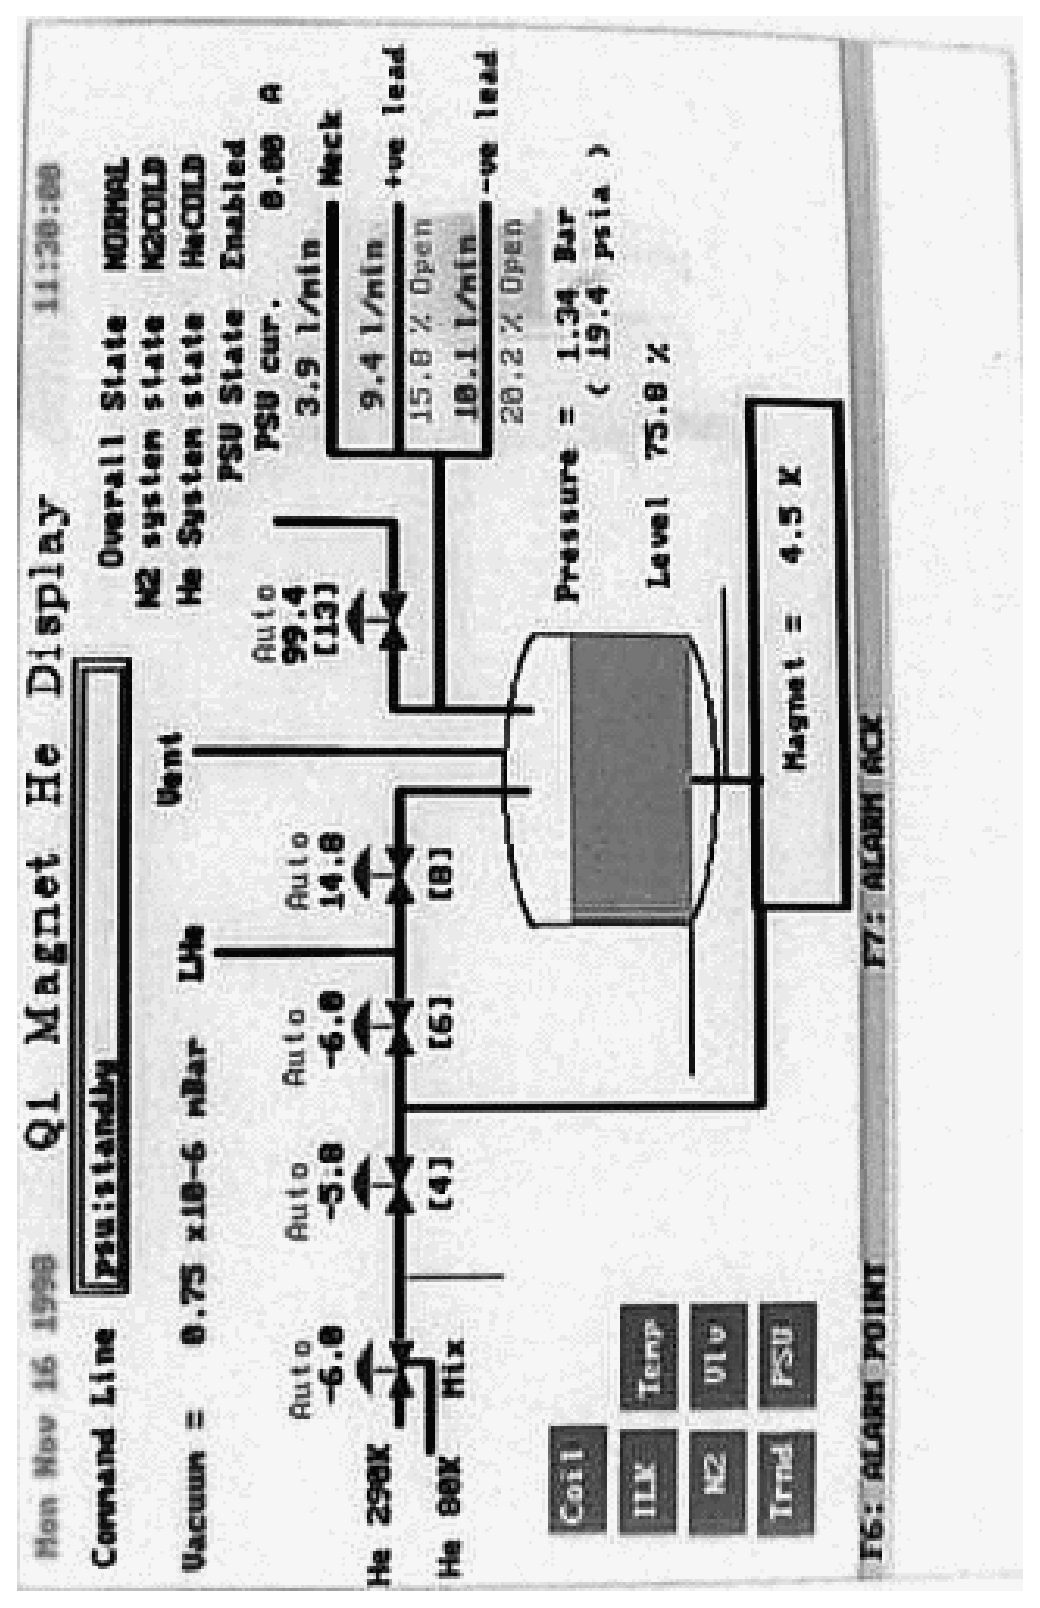
\includegraphics[angle=-90,width=4in]{spectrometers/Q1-helium.ps}
\caption{Sample Helium Monitoring Page - Q1\label{fig:he_page}}
\end{figure}

\begin{figure}
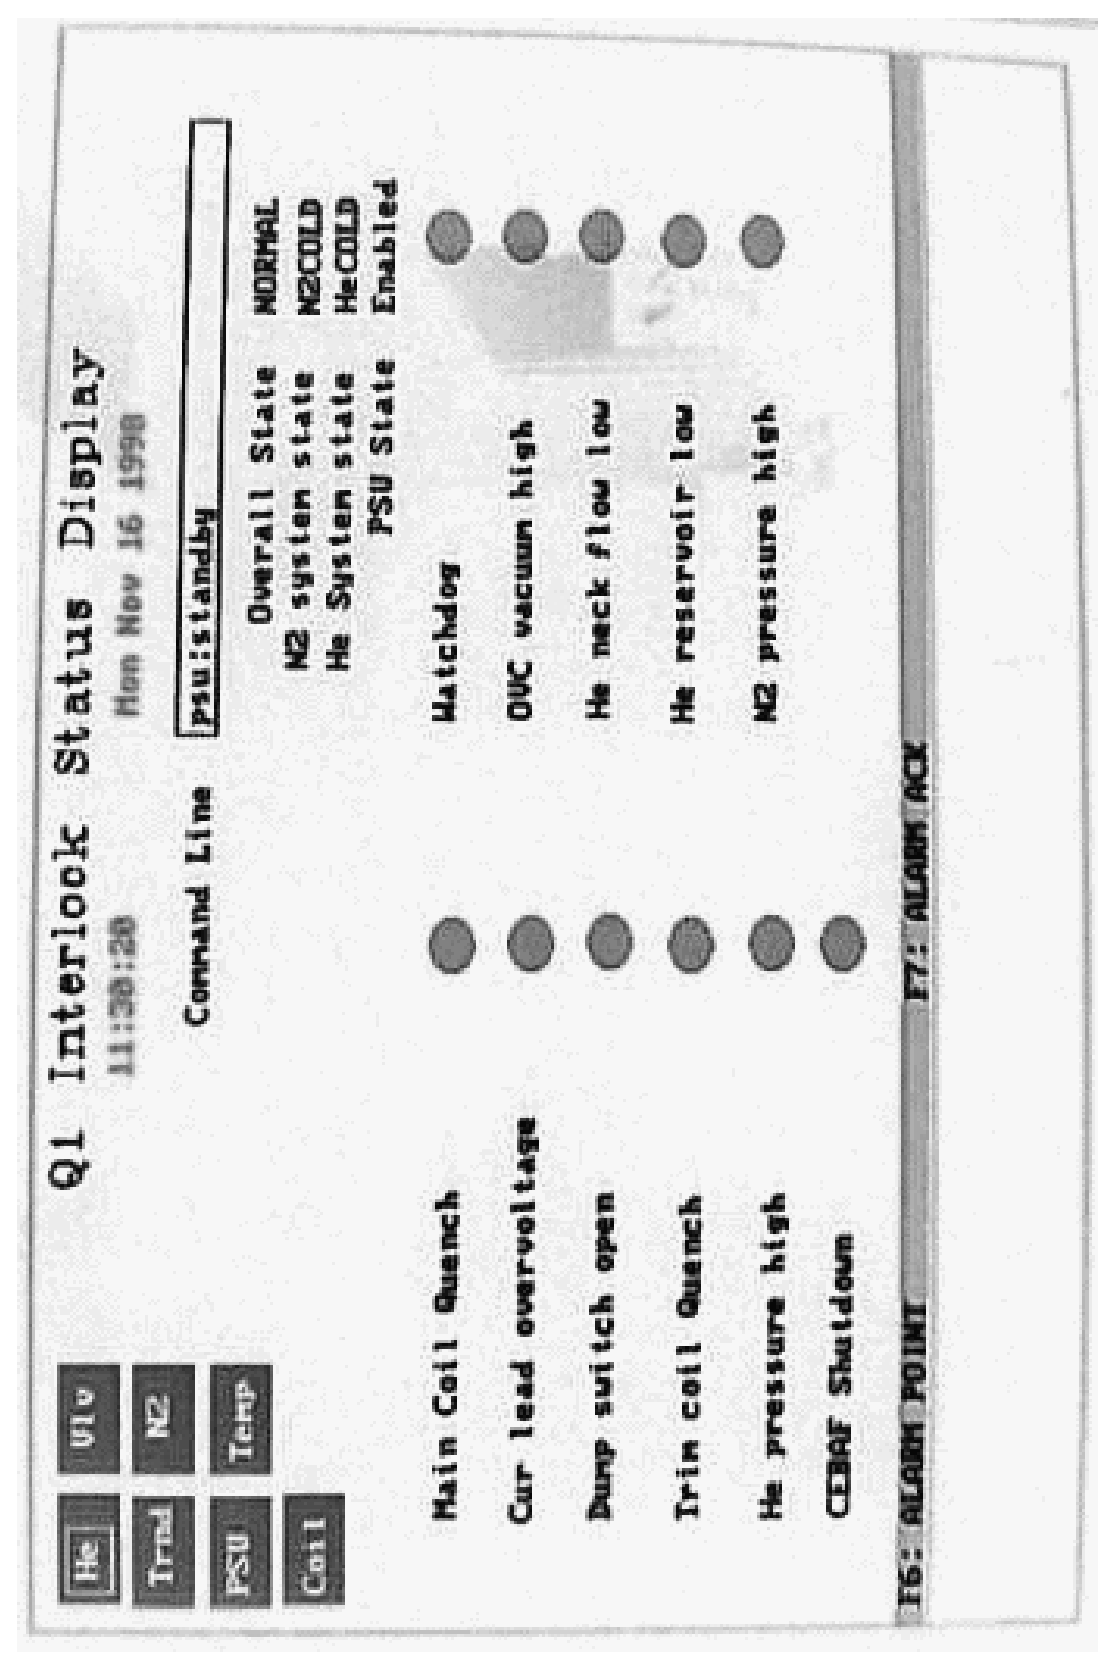
\includegraphics[angle=-90,width=4in]{spectrometers/Q1-interlock.ps}
\caption{Sample Nitrogen Monitoring Page - Q1\label{fig:nit_page}}
\end{figure}

\begin{figure}
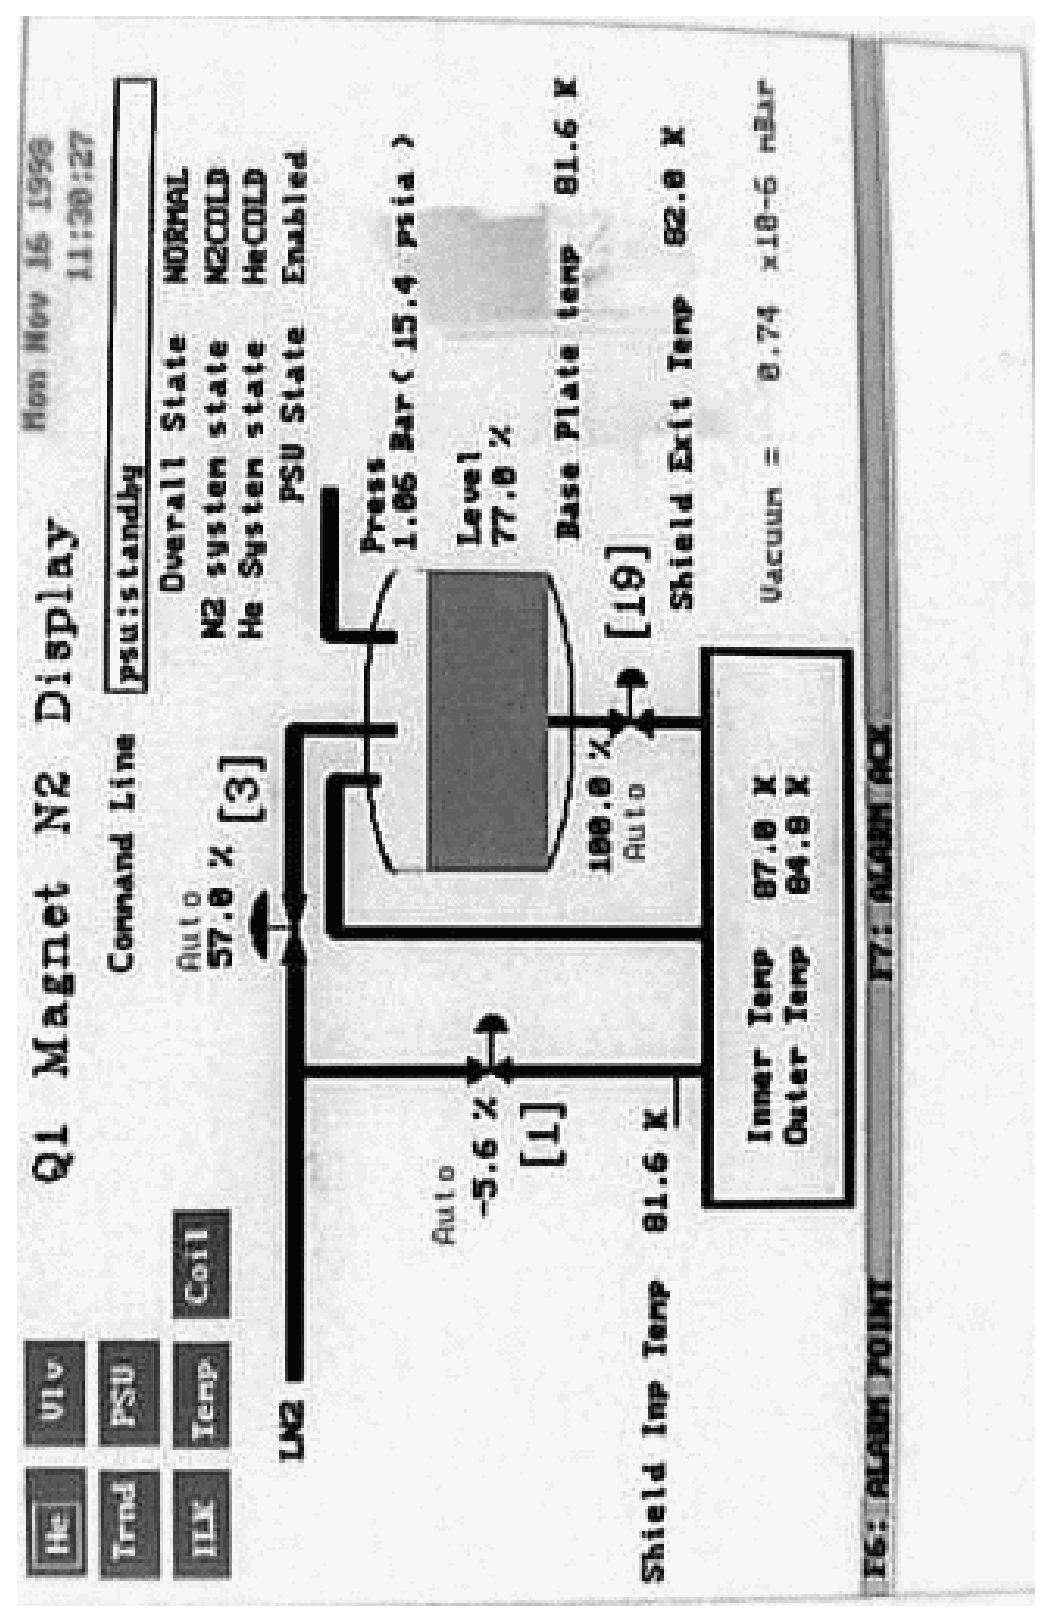
\includegraphics[angle=-90,width=4in]{spectrometers/Q1-n2.ps}
\caption{Sample Power Supply Monitoring Page - Q1\label{fig:ps_page}}
\end{figure}

\begin{figure}
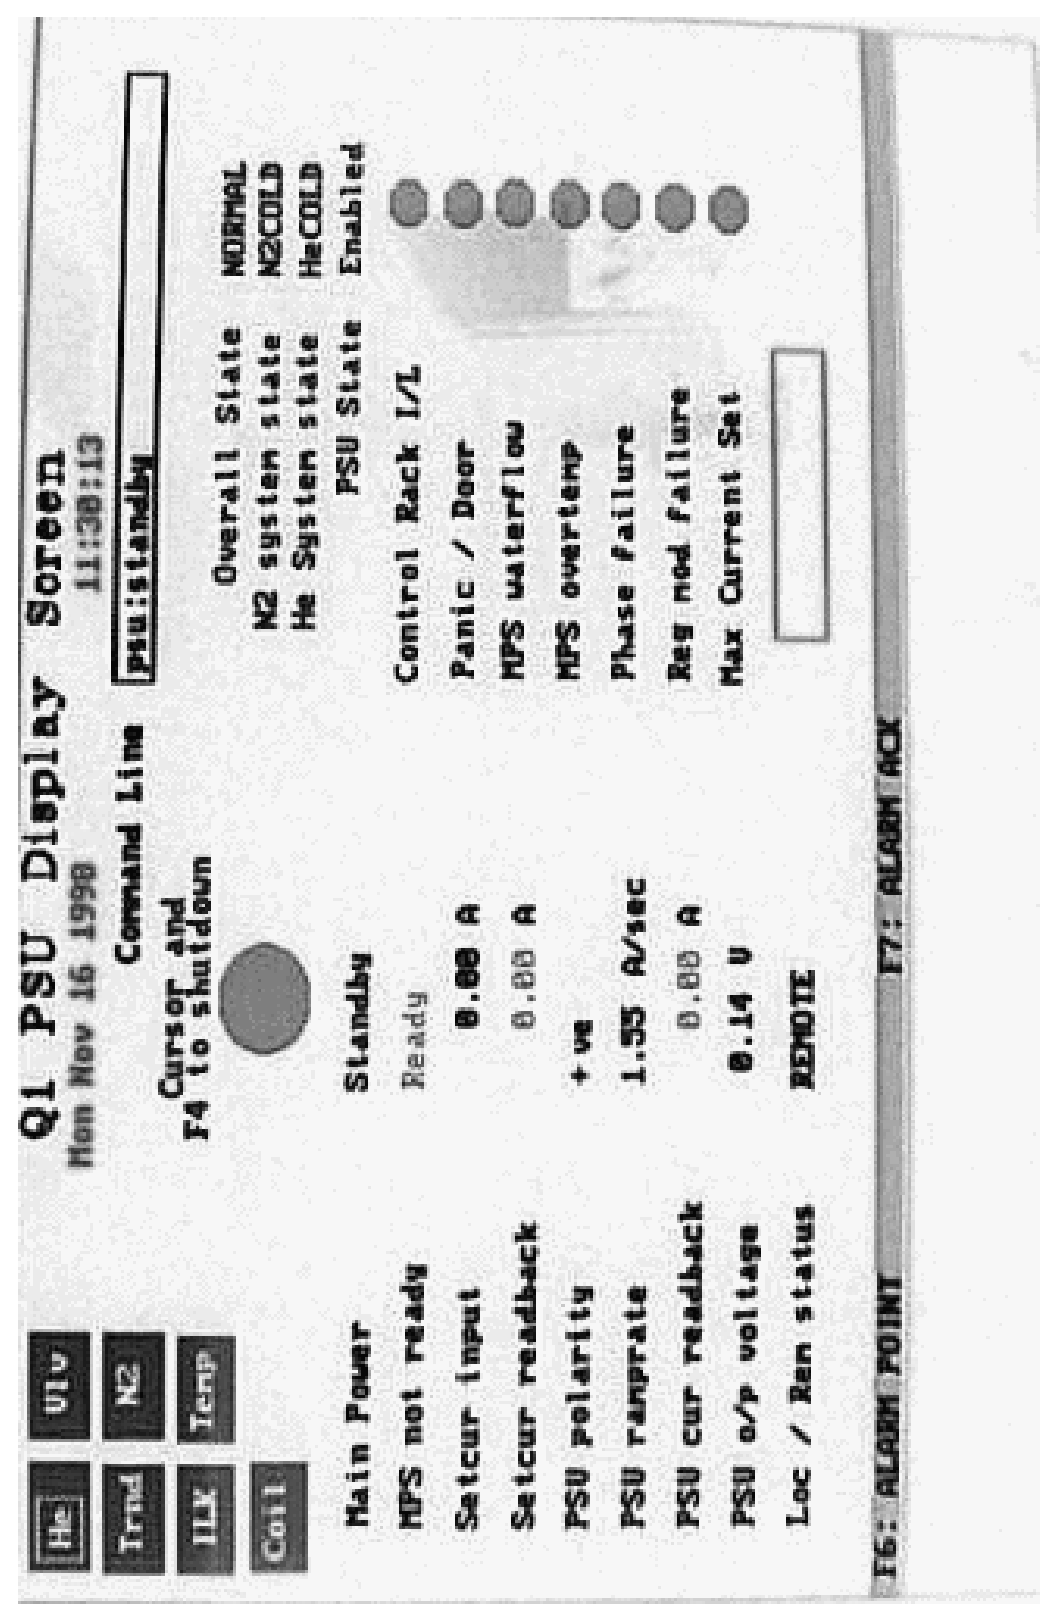
\includegraphics[angle=-90,width=4in]{spectrometers/Q1-psu.ps}
\caption{Sample Interlock Monitoring Page - Q1\label{fig:is_page}}
\end{figure}

\begin{figure}
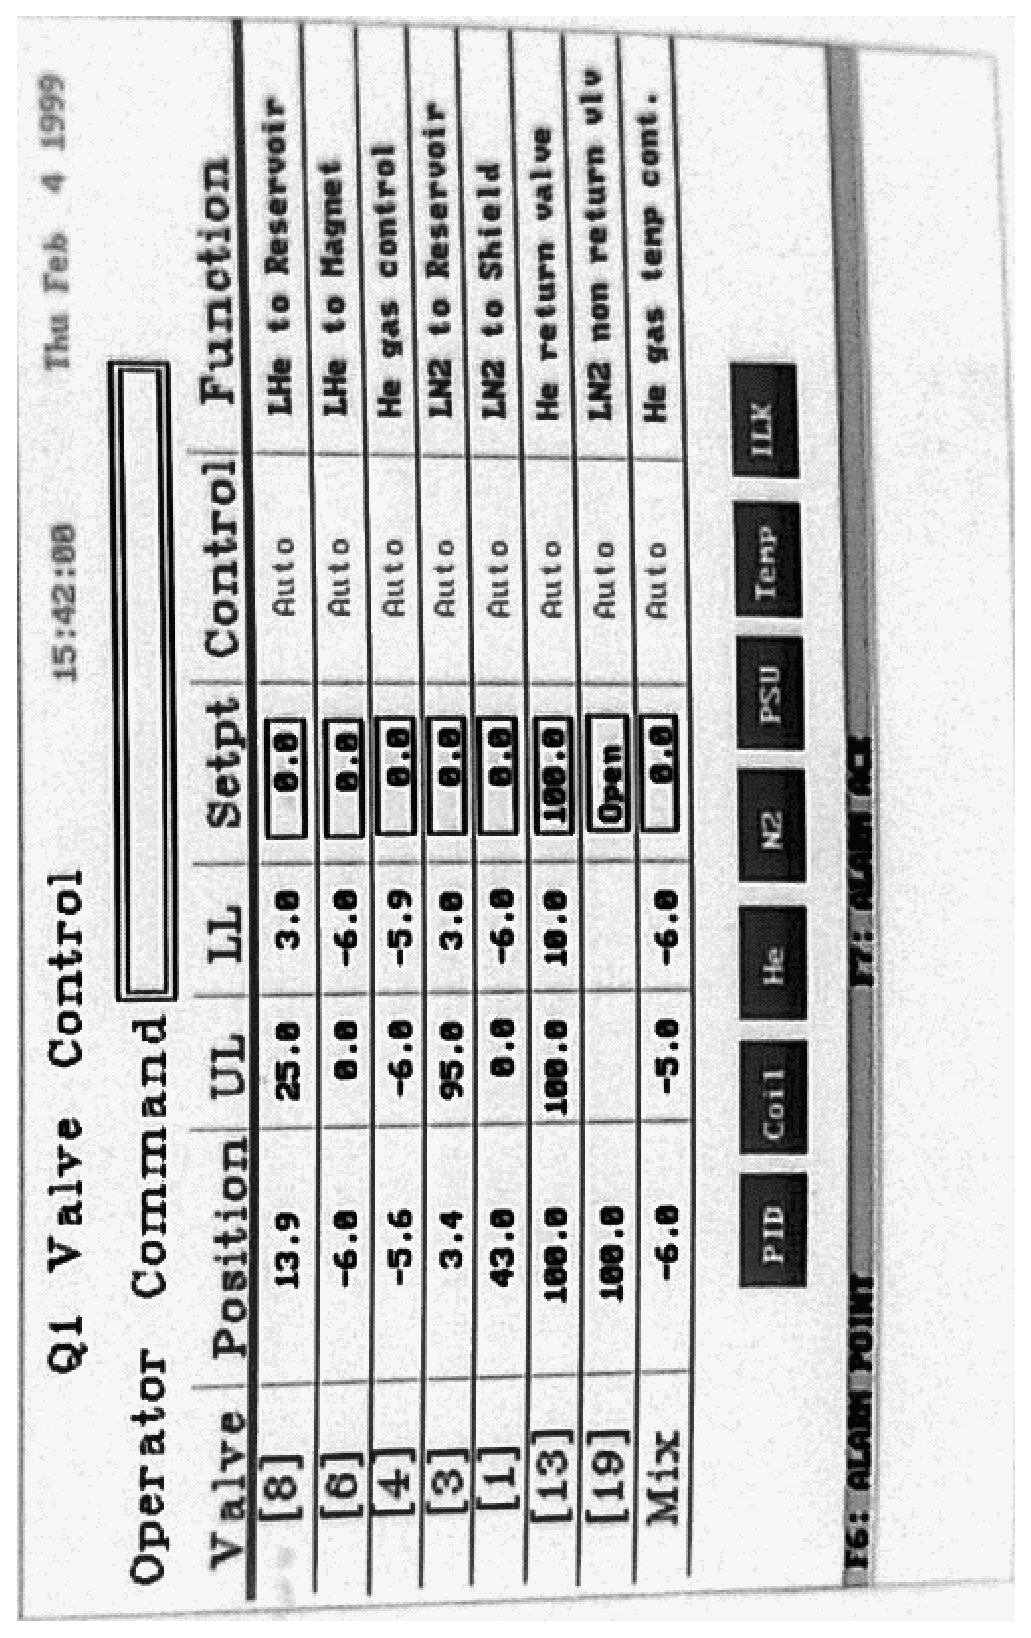
\includegraphics[angle=-90,width=4in]{spectrometers/Q1-valves.ps}
\caption{Q1 Valve Control Page\label{fig:q1_valve_page}}
\end{figure}

%\begin{figure}
%\vspace{8.0in}
%\caption{Q1 Valve Control Page\label{fig:q2_valve_page}}
%\end{figure}

%\begin{figure}
%\vspace{8.0in}
%\caption{Q3 Valve Control Page\label{fig:q3_valve_page}}
%\end{figure}

\begin{figure}
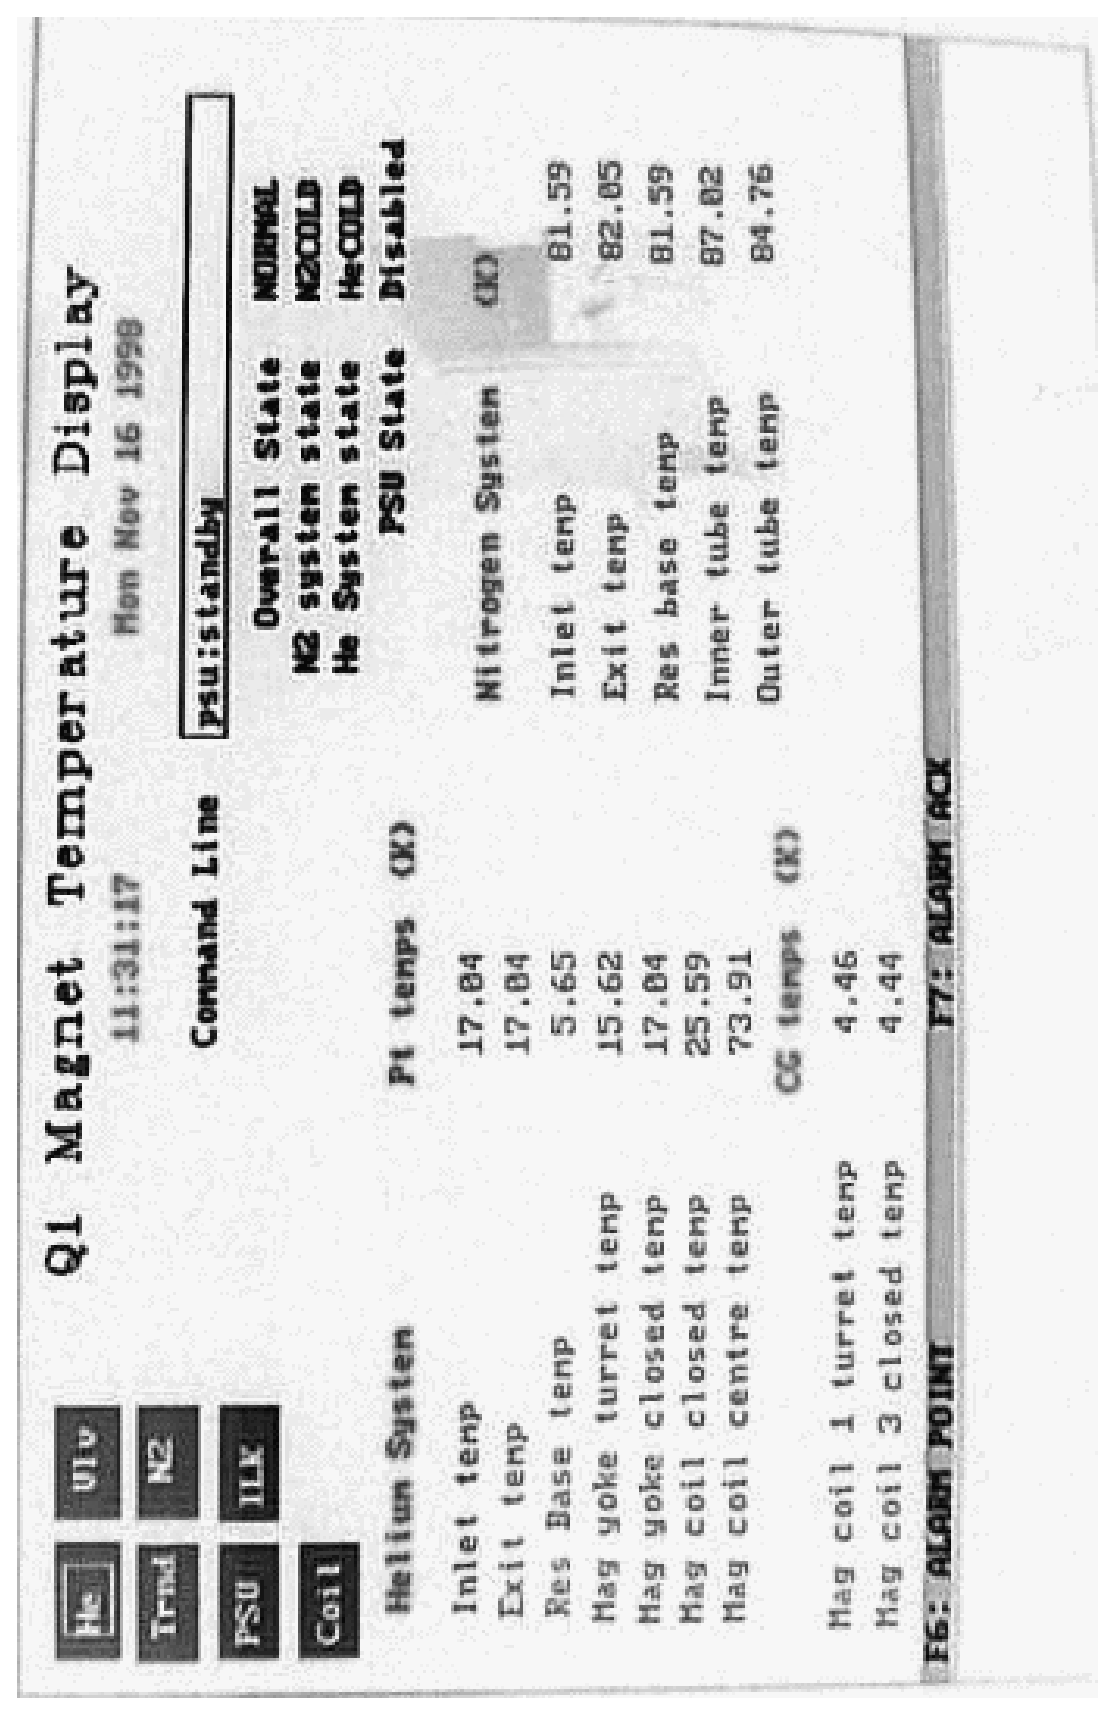
\includegraphics[angle=-90,width=4in]{spectrometers/Q1-temps.ps}
\caption{Sample Magnet Temperature Display - Q1\label{fig:temp_page}}
\end{figure}

\begin{figure}
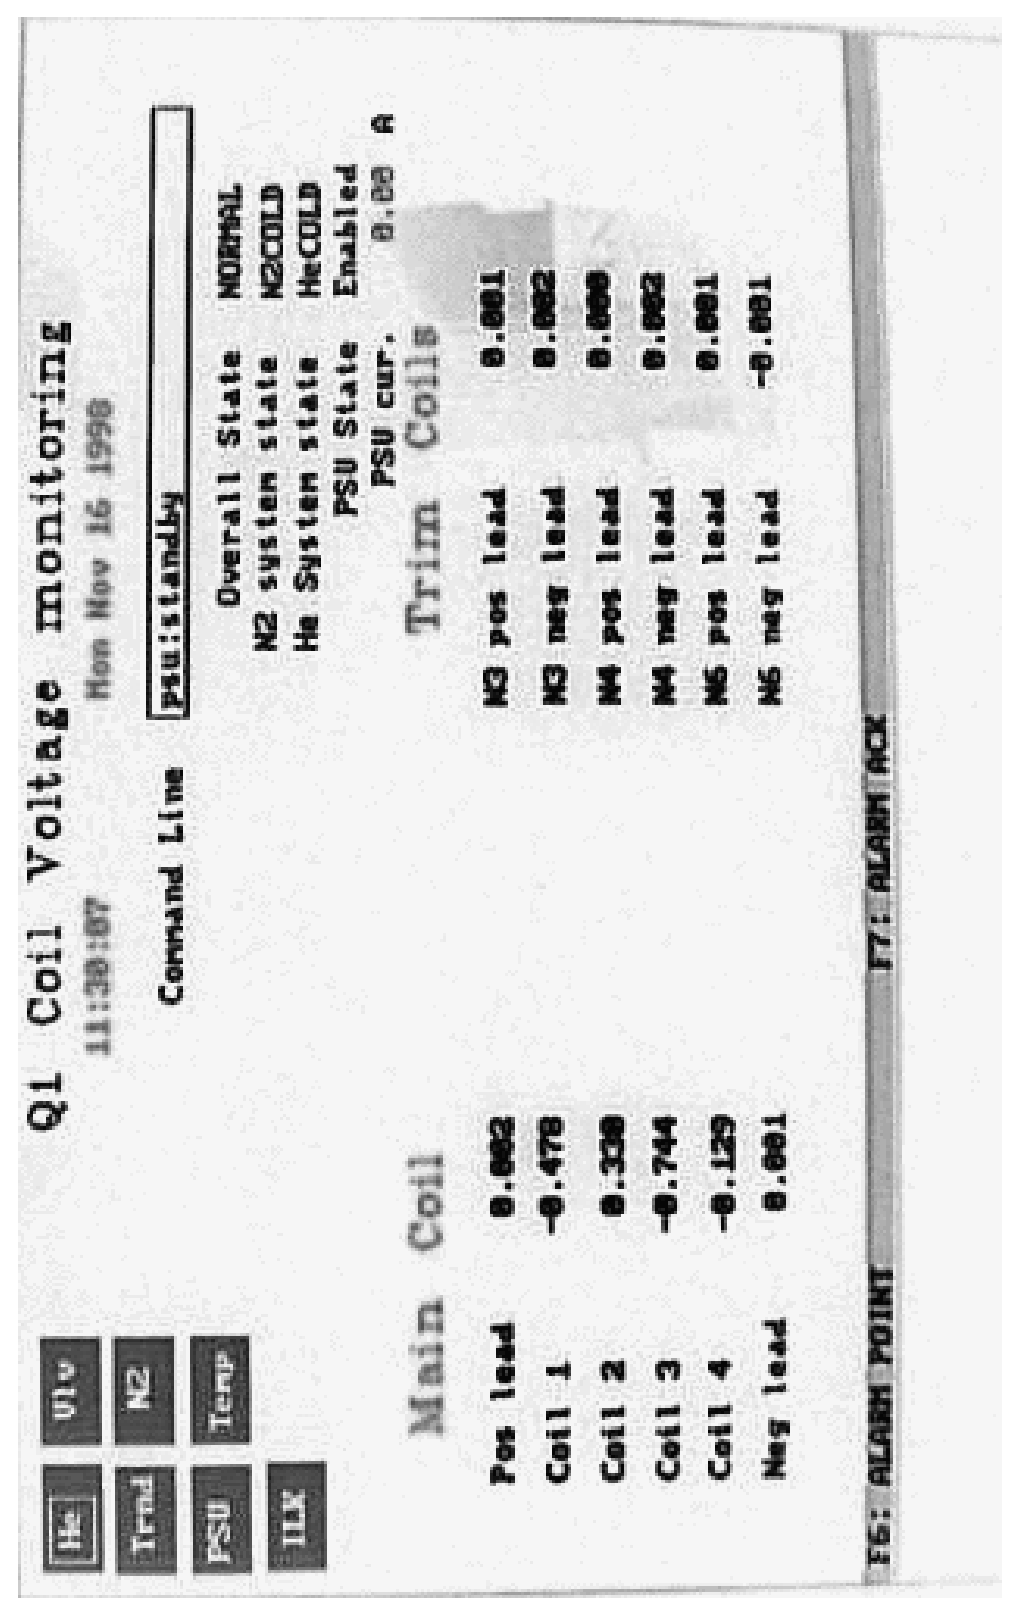
\includegraphics[angle=-90,width=4in]{spectrometers/Q1-voltage.ps}
\caption{Sample Coil Voltage Monitoring Page - Q1\label{fig:coil_page}}
\end{figure}

\begin{figure}
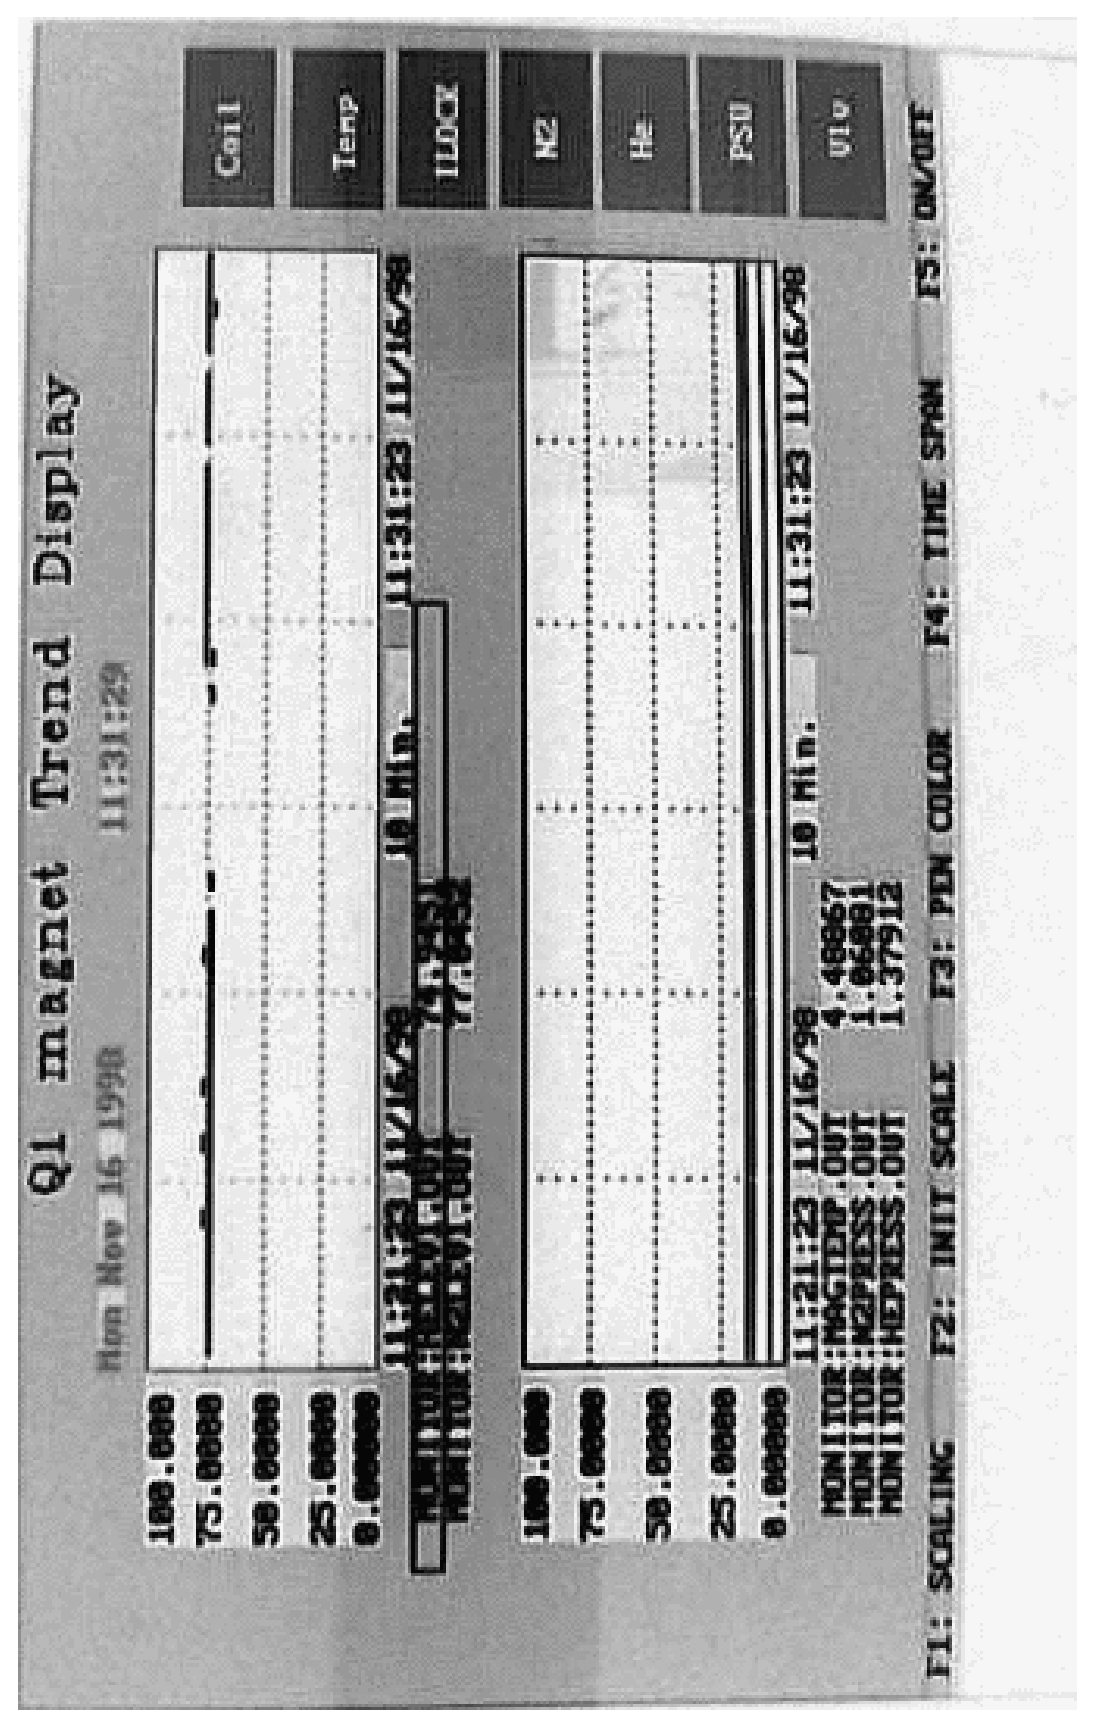
\includegraphics[angle=-90,width=4in]{spectrometers/Q1-trend.ps}
\caption{Sample Trend Page\label{fig:trend_page}}
\end{figure}

\end{center}

\medskip

\begin{description}
\item[B.] {Dipole Pages}
\end{description}

\begin{description}
\item{}\hskip0.1in {[F1] Main Menu}
\item{}\hskip0.5in {Cooling (Cooldown Menu)}
\item{}\hskip0.5in {Field Regulation (NMR Controlled Programmed Ramp)}
\item{}\hskip0.5in {NMR Manual Operation (Field Control)}
\item{}\hskip0.5in {MPS Manual Operation (Current Control)}
\item{}\hskip0.1in {[F2] Coil Temperatures}
\item{}\hskip0.1in {[F3] Shield Temperatures}
\item{}\hskip0.1in {[F4] Cryogenic Page}
\item{}\hskip0.1in {[F5] Strain Gauge Page}
\item{}\hskip0.1in {[F6] Voltage Page}
\item{}\hskip0.1in {[F7] RS232 Status Page}
\end{description}


\subsection{HMS Vacuum System}

	The spectrometer contains five separate vacuum volumes.
These are the isolation vacuums of each of the superconducting
magnets and the main spectrometer volume through which the particles
to be detected travel.

The isolation vacuums are normally cryo pumped by the cold mass when the
magnets are cold and hence have no mechanical pumps
associated with their maintenance. They also have no thin
windows or other hazards and will not be discussed further in this document.

The main spectrometer vacuum
is currently maintained by the two mechanical pumps.
One pump is located between Q3 and the Dipole on the small angle
side of the carriage while the second pump is the backing
pump of the turbo and pumps the spectrometer volume through the turbo.
Presently we do not use the turbo pump to pump the spectrometer volume due to
the high leak rate through the large rear vacuum window in the shield house.
This mechanical pump is located
at the back of the carriage and the turbo is located in the shield house
underneath the end of the vacuum can that protrudes into the detector hut.

The vacuum in the spectrometer may be read out on a gauge that is sitting on the
carriage beneath Q3. There is a TV camera that views this gauge readout and
it is displayed on one of the TV monitors above the console in the hall
C counting house. The absolute value of the vacuum is not the quantity
of interest (until we improve window technology) but rather its rate of change.
Thus far we have maintained fairly stable vacuum over the course of each run
period and if things are functioning normally we should continue to do so.
If the vacuum starts to deteriorate rapidly an expert should be notified.



\subsection{HMS Slit System}
\label{sec:hms_slit}

The HMS slit system is installed on the gate valve housing mounted to the
front face of Q1. It consists of a vacuum box with a slit ladder
mounted into it. The slit ladder has space for three separate slits,
which will typically be one sieve slit and two solid angle defining collimators.
The slits are rectangular blocks of densimet (90\% W and 10\% Cu/Ni)
with a density of 17 g/cm$^3$. The collimators have an octagonal shaped
opening machined into them; the sieve slit has many holes drilled
into it.

The outer size of the collimators is 11.75" vertical by 8.25"
horizontal. The outer size of the sieve slit is 10.00" vertical
by 8.25" horizontal.
Its vertical size is reduced w.r.t. 11.75" due to space constraints.
The sieve slit always has to be installed at the bottom position of the ladder,
so that we can use the shielding of the collimator above it to
clearly distinguish the top row of holes. The central hole
of the sieve slit has a smaller aperture, and two blocked holes
exist to easily distinguish center and directions.
The collimator thicknesses are 2.5", while the sieve slit thickness
is 1.25". The dimensions and shape of the inner aperture of the present
HMS collimators is denoted in Table~\ref{tab:apertures}.

\begin{table}
\begin{center}
\caption{Apertures of Collimators\label{tab:apertures}}
\vspace{\baselineskip}
\begin{tabular}{|c|c|c|c|c|c|}
\hline
{} & {} & {} & {} & {} & {} \\
HMS/SOS & d$\Omega$ & Horizontal & Vertical & Shape & Note \\
{} & (msr) & (mr) & (mr) & {} & {} \\
{} & {} & {} & {} & {} & {} \\ \hline
HMS & 6.74 & $\pm$ 27.5 & $\pm$ 70.0 & Octagonal, Flared & Quads Nominal \\
HMS & 6.74 & $\pm$ 27.5 & $\pm$ 70.0 & Octagonal, Flared & Quads Backward \\
{} & {} & {} & {} & {} & {} \\
SOS & 7.55 & $\pm$ 57.5 & $\pm$ 37.5 & Octagonal, Flared & \\
SOS & 3.98 & $\pm$ 32.5 & $\pm$ 35.0 & Octagonal, Flared & \\
\hline
\end{tabular}
\end{center}
\end{table}

The total depth of the slit box is close to 3.75", which leaves
enough space to later mount scintillators behind the collimators as an active
veto counter (to prevent punch-through of hadrons) and/or to increase
the collimator thickness. Two circular quick-connect flanges are
added for feed-through of possible light guides.

\subsubsection{Operation of the HMS Slit System}\label{sssec:slit_control}
A remote control system consisting of motor/actuators exists to slide
the slits into place. Resolvers specify the exact position of the
slits.  The control box is located downstairs in Hall~C, behind the
blue power supply racks. On the front face there are four buttons for
each spectrometer. These indicate the three different slit positions
and the ``home" position, which denotes that no slit is used at all
(slit ladder in the up position).  Brake cables are added to prevent
the slit ladder from falling in case of a power loss. Next to this an
emergency button is included to electrically shut down the control
system.

{\bf After a power cycle the HMS slit moves itself to the {\it HOME} position,
returning a reading of 0. Thus, after a power failure or other cycle, the slit
must be commanded to a meaningful position using the commands described below.}

Normally, the system is operated remotely. Connect to the controller
using terminal server hctsv7, port 3:

\begin{minipage}{6in}
\begin{enumerate}
\item telnet hctsv7 2003
\item type {\tt \verb|\B|} to connect to HMS, {\tt \verb|\A|} for SOS. (Must be UPPER CASE)
\item {\tt P PFB} gives readback of the current position (see Table \ref{tab:col_pos})
\item To {\em MOVE} the collimators:
   \begin{itemize}
	\item {\tt EN} - to enable motion.
	\item {\tt RUN 10} - follow instructions (see slit numbers and postions at bottom)
	\item After you have reached the correct slit, disable the motor by typing {\tt 1}

   \end{itemize}
\item If necessary, {\tt K} (kill) is the opposite of {\tt EN}
\item Get rid of your session by typing {\tt \verb|ctrl-]|} (both pushed together), then
at the telnet prompt, type {\tt quit}.
\end{enumerate}
\end{minipage}

Don't forget to get rid of your session. If you do not close your session nobody
else can communicate with the slit controllers.

\begin{table}[!ht]\
\caption{Slit Collimator Positions\label{tab:col_pos}}
\begin{center}
\begin{tabular}{rlrr}
   &                  &     HMS   & SOS\\
\hline
1) & Sieve Slits      &  19804600 &  11638719\\
2) & Large Collimator &       N/A &   3190717\\
3) & Pion Collimator  &  -3096800 &       N/A\\
\end{tabular}
\end{center}
\end{table}
   
\subsubsection{Hazard Identification}

The principal hazards are:
\paragraph{Magnetic:} There is a significant fringe field at
the entrance and exits of the magnets. This represents a hazard
to people working on the slit system if they are handling magnetic
objects (tools) or to people with pacemakers. In addition the field could erase magnetic
information storage media such as the strips on credit cards.
\paragraph{Mechanical:} At the front of Q1 the housing for a spring loaded gate valve is
mounted. In its normal operation mode a metal gate will be closed with
severe pressure when the electrical power drops. This can cause serious
damage to interfering body parts.  But currently the shutter and
actuator have been removed so this hazard does not exist.  
A similar mechanical problem involves the slit ladder itself. The total weight of
the three slits amounts to approximately 350 Lbs (160 Kg) and can easily
cause serious damage to body parts.

\subsubsection{Hazard Mitigation}

\paragraph{Magnetic}

A sign will be posted which indicates the presence of a high magnetic
field ( this is standard JLab safety signage). The exact wording is
`` High Magnetic Field - No Pacemakers or Credit Cards." There are also
flashing red lights located on the HMS carriage indicating that the
magnet power supplies are energized. Be careful with tools (are they magnetic?)
when you work on the slit boxes with the red lights in a flashing state.

\paragraph{Mechanical}

If the gate valve is ever re-installed, the following safety
procedures should be observed.  Without power, the gate valve assumes its default closed position due to
pressured air. When installing the slit boxes, or working with your hands
in the vicinity of the inside of the gate valve, disconnect first the power
plug of the gate valve, such that the gate valve closes.
In case you need the gate valve to assume a default open position without
power, first relieve the air pressure
with power on, and verify that the default position of the gate valve has
changed to ``open" by removing the power. Paul Hood (x7849) or Mike Fowler
(x7162) can be contacted for more information.

When installing the slit ladder, be careful when you work with your hands
under the slit ladder (like when you are bolting the slit box to the
gate valve). Remove the slit ladder, or {\bf install a support under the slit
ladder to prevent it from falling all the way down}.

A brake system has been included in the control to prevent the slit ladder
from sliding down in case of a power failure.  However, this must not
be relied upon for personnel safey.


\subsection{HMS Carriage and Rotation System }

	The Carriage is the support structure of the spectrometer.

First and foremost as it is a multi leveled structure it is important to keep in
mind that people may be working above you. This means that hard hats should
be worn.

There are two sets of steps on the carriage. The first set of steps
(closer to the pivot, leading to the power supplies) is very
steep (almost like a ladder) and hence extra care should be exercised
while using this set of steps. The second set of steps is at the rear
of the carriage and provides access to the main level as well as to
the catwalk and shield house. Taller individuals should be mindful
when using this flight of steps due to the limited head room at some 
points.

The first level of the carriage is almost at beam height and therefore
the usual precautions associated with working at heights should be followed (note:
safety railings have been installed everywhere possible along the carriage
perimeter, but there may still be unprotected spaces as conditions change).

The entire spectrometer can be rotated. Currently, the angle of the spectrometer
is found using a plumb bob attached to a reference mark on the
carriage frame under the ``pasta fork" at the rear of the spectrometer.
This plumb bob is aligned over survey marks which have been painted
on the floor in red and scribed at 0.5 degree intervals. Rotation of the spectrometer
is accomplished by using the two motors on the carriage itself (the motors on
the shield house bogies are not used in the present rotation system).
These AC motors are controlled by synchronous pulse width modulated
drives which are mounted near the bottom of the shield house steps.

\subsubsection{Remote Rotation}

Cameras are installed to enable readout of the HMS spectrometer angle
(using the plumb bob and the survey marks on the floor).

The wide-lens and zoom cameras located at the entrance and
the exit of Hall~C should be used to visually spot for obstructions
before and during remote rotation.

Limit switches are installed at forward
and backward angles which prevent HMS from rotating to angles more forward than
10.6 degrees and more backward than 85 degrees. To obtain more forward or more
backward angles an access is needed, and rotation has to occur manually
downstairs with spotters. Hard limit switches will be installed to prevent
the spectrometer from rotating out of maximum allowed range.

In case the HMS spectrometer is rotated to more forward angles, pay special
attention to possible interferences of HMS and SOS. Up to this moment
the closest  angle distance we have obtained between SOS and HMS is 28 degrees.

Remote rotation  is accomplished via the PLC located in the Hall.  It
is currently installed in the HMS shield hut for protection from
radiation.  Commands can be issued to the PLC (Texas Instruments 5000), which executes these commands
following algorithms stored in its memory. An EPICS screen is now
used to talk to the PLC.  The advantages of using the PLC are:

\begin{itemize}
\item{No direct access by users to the algorithms, preventing unsafe
rotation attempts (instead, the algorithms have to be loaded locally into
the PLC).}
\item{Rotation of both HMS and SOS by the same smart controller, enabling
security checks of both angle decoders. This renders a better handle on the
minimum allowed angle between the two spectrometers.}
\item{Automatic slower rotation speeds (if desired) if close to desired angle
when using proximity switches.}
\end{itemize}

The PLC communicates directly with the control electronics of several limit
switches, proximity switches, and decoders. Next to the limit switches
also hard limit switches will be installed on the floor to mitigate failure
of the PLC limit switches.


\subsubsection{Personnel Trained for Manual Spectrometer Rotation}

The spectrometer motors may only be controlled by trained personnel.
At least two people are required for spectrometer rotation, one to
run the motors and at least one spotter. Prior to rotating the spectrometer
a visual inspection of the area should be made to insure that there
is nothing in the spectrometer's path or on the rails. During rotation
the spotter should pay special attention to
the cables which run from the
spectrometer to the target motor controller to make sure that
nothing is hung up or stretching.

In case you need to rotate the spectrometer manually, contact one of the trained
personnel listed in Responsible Personnel (chapter 4) in
the \htmladdnormallinkfoot{ESAD}{http://www.jlab.org/Hall-C/document}.

\section{Short Orbit Spectrometer (SOS) }

The SOS is composed of one quadrupole and two dipole magnets.
These are all conventional resistive magnets and are powered by standard
power supplies.
The first dipole deflects particles by 33 degrees, while the
second dipole deflects by 15 degrees in the opposite direction, such
that the total bend of the SOS dipoles is 18 degrees.
The two dipole magnets are enclosed in a common yoke.

The SOS quadrupole was assembled at Argonne National Laboratory and
subsequently shipped to JLab. The dipole is a copy of the Medium Resolution
Spectrometer of Los Alamos, and has been assembled at JLab by a collaboration
of Argonne National Laboratory, Los Alamos, and JLab.

The magnet system is followed by a large concrete detector (or shielding) hut,
in which all detector elements can be found. All of these
detector elements have been built by universities and laboratories involved 
in the Hall~C
physics program.

The SOS magnet system combines a large acceptance (solid angle and momentum
acceptance) with a relatively short path length to the focal plane.
The primary object of this spectrometer is to detect short-lived particles
like pions and kaons. In addition, a large fraction of the experimental
program in Hall~C requires a spectrometer with large momentum and solid angle
acceptance to maximize the operational efficiency.
The maximum central momentum attainable with the SOS magnet system is 1.8 GeV/c.

\subsection{SOS Magnets and Power Supplies }

The SOS magnets are powered by large supplies
(160 Volt, 1000 Amps for Quad and D2, 250 Volts, 1000 Amps for D1).
When working on the power supplies, the responsible people will follow
the guidelines in the electrical safety chapter of the `` JLab EH$\&$S
Manual." Further references which should be consulted before power supply
maintenance or operations are attempted are the operating procedure
provided by the manufacture (Inverpower) and the simplified magnet
power supply maintenance procedure.
The connections at the quadrupole are covered with a 1/4 plexiglass, so that they are not exposed.
The cabinet doors for the power supplies are locked.
There is also a crash button in the counting house which is interlocked with
a separate key. When the key is locked off, in crash mode, the power supply
cannot be energized.
In case you need any of the keys, see the Responsible Personnel listed in 
the \htmladdnormallinkfoot{ESAD}{http://www.jlab.org/Hall-C/document}.

Signs have been posted which indicate the presence of a high magnetic
field ( these are standard JLab safety signage). The exact wording is
``High Magnetic Field - No Pacemakers or Credit Cards." There
are also flashing red lights located near the exit of the last dipole
and near the entrance of the dipole at the pivot that indicate that the
magnet power supplies are energized.

The magnets and their power supplies
are cooled by the Hall~C Low Conductivity Water system (LCW).
The LCW system for the dipole and quadrupoles has been
plumbed using hoses rated for 600 PSI. These hoses have been tested during
the magnet mapping. The cooling water is delivered at 240 PSI.

The spectrometer is in Hall~C and the power supplies are located
behind the blue electronics racks on the HMS side of the hall.
The control of the magnets is available through VME, and will be
described in a subsequent Section.


\subsubsection{SOS Magnet - Description}

The SOS consists of 3 magnets: a quadrupole (QS), followed by two dipoles housed
in a common yoke (BM01 and BM02). All three are resistive magnets
with pressurized water cooling. They are powered by 3
InverPower remotely controlled power supplies, located in the blue racks at
the north side of Hall~C. Group-3 Digital Tesla meter hall probes
are used to monitor the magnetic fields.

The magnets are aligned as a vertical-bend Q, D, -D spectrometer: BM01 bends
charge=1 particles of the central momentum upwards by 33 degrees, and BM02 bends
the central ray down by 15 degrees, resulting in a slope of 18 degrees through
the detectors. QS focuses in the non-bend plane, and defocuses in the bend
plane. Focusing in the bend plane is provided by the dipoles, which have tilted
and curved entrance and exit edges. The ``standard" tune has first-order
point-to-point focusing in both the bend and non-bend planes at the ``standard"
reconstruction plane, located approximately at the first drift chamber (DC1).
An alternate tune with parallel-to-point focusing in the non-bend plane can be
achieved by lowering the excitation of QS and changing the location of the
focal plane. The power-supplies contain a motorized internal bus that can 
reverse
the output polarity so that operation for either positive or negatively charged
particles is possible.

Both BM01 and BM02 require an asymptotic field (far from the edges) of 11379.3
Gauss/GeV for the central ray. While the center of BM01 is far from the edges,
BM02 is a thin magnet, and there is no region that isn't close to the entrance
and exit edges. The proper relative excitation of these magnets is determined
by numerically integrating the central ray's trajectory through the fields
measured during the mapping of these magnets, and by comparing the observed and
expected trajectories of the central ray through the drift chambers.

The ``standard tune" requires a gradient of approximately 498.152 Gauss/cm/GeV
in QS. The excitation of QS relative to BM01 was determined by observing
electrons that passed through a sieve-slit mask at the entrance to QS after
scattering elastically from a carbon target. The field in QS was varied until
the correct focus was observed at the reconstruction plane.

The maximum central momentum of the spectrometer is approximately 1.75 GeV.
This limit is imposed by the power supplies; at this setting BM01 requires
approximately 1000 amps, and QS requires approximately 170 volts. 
Table~\ref{tab:sos_ratings}
lists the maximum output voltage and current of each power supply. However, the
iron in the magnets is significantly saturated at this setting, and a 
significant
increase in the central momentum probably can't be achieved without affecting
the optics.

\begin{table}
\begin{center}
\caption{Maximum ratings of SOS power supplies. \label{tab:sos_ratings}}
\vspace{\baselineskip}
  \begin{tabular}{lll}
Magnet         &Max Current    &Max Voltage    \\
                     &~~~~~(A)        &~~~~~(V)              \\
\hline
BM01           &1000 (*)       &250            \\
BM02           &1000           &160            \\
QUAD           &1000           &160 (**)       \\
\end{tabular}
\end{center}
\noindent{(*)  Limits max momentum setting of spectrometer}\newline
\noindent{(**) The quad is driven to $\approx$170 volts at 1.75 GeV, but this
is within the overdrive capability of the supply.}

\end{table}

All three magnets are equipped with Group-3 precision hall-effect probes to
monitor their fields. BM01 and BM02 are equipped with LPT-141 probes that are
glued onto the pole tips inside the magnet vacuum with Torr seal epoxy. The cables
from the probes are routed inside the magnets to the transition vacuum piece
between QS and BM01, where they pass through a feed-through. The BM01 probe was
placed near the center of the pole, in the uniform field region. The BM02 probe
was placed near the widest part of the pole. in both cases, the probe location
is outside of the beam envelope accepted by the spectrometer.

QS is equipped with a LPT-130 probe located in an aluminum holder mounted in an
access hole of one of the stainless-steel spacers between the upper and lower
pole pieces. This positions the probe in the horizontal midplane of the magnet,
in the region where the upper and lower pole pieces are closest together. The
field at this point is proportional to the field gradient in the magnet bore, in
the absence of saturation. Saturation effects are estimated by the 2D magnet
code Poisson, but the precise tune of the magnet relative to BM01 can only be
determined experimentally.

The cables for all three hall-probes are bundled together at the transition
piece between QS and BM01. The cables for BM01 and BM02 have a connector that
attaches to the feed thrus on the top of the transition piece. (There is a
corresponding connector inside the magnet vacuum.) The feed thru for BM01 is
the one closest to the target. It is extremely important that the external
connections for BM01 and BM02 not be interchanged. This is because the cables
terminate in a small connector containing a PROM with the calibration table for
that specific probe. Although the probes will operate with the wrong cable, the
field values will be incorrect. The cables, connectors, and feed thrus are
labeled for correct assembly.

The bundled hall-probe cables are routed back through the dipole yoke, around
the inside of the shield house, and through the rear-wall penetrations to the
electronics shack. The readout-electronics are located in one of the lefthand
relay racks, as one stands facing the target. BM01 and BM02 probes are connected
to DTM-141 units, QS is connected to a DTM-132 unit. These units are
daisy-chained together with a fiber-optic link, and communicate with crate
VMEC9 via an RS232 serial I/O port.

\subsubsection {SOS Magnets - Operation}

IMPORTANT: Before any power is applied to the magnets, you must make sure that
the cooling water is flowing through them. There are two circuits controlled by
the spectrometer water-rack located near the spectrometer pivot. One supplies
water to QS, and is labeled TEST. The other supplies both BM01 and BM02; it's
labeled SOS. Visually check the flow gauge.
%Typical values are ??? for QS and ??? for SOS.
Refer to the section on the LCW system for the procedure to turn the water on and off.

IMPORTANT: The SOS power supplies are themselves water cooled, and you must
make sure that the cooling water is flowing through them before energizing
their AC power circuit breakers. The water rack for the power supplies is
located immediately to the left of the power supplies as you face their front.
Refer to the section on the LCW system for the procedure to turn the cooling water on and off.
Visually check the flow gauge.
%typical values are ??? for QS, ??? for BM01, and ??? for BM02.

The SOS power supplies may be controlled either locally through their front
panel, or remotely by computer. The normal mode of operation is by computer.

Remote control of the power supplies is performed through an interactive
computer program run on VME crate VMEC19. To access the controls, telnet to
vmec19.jlab.org. As a security precaution, telnet access is only allowed
from Hall C computers, and you must login with a username and
password.  The username and password are available
from Steve Wood on request.

Once logged in, the control program is started by the command ``sos".  This
results in a display of the current power status, plus a prompt for a
command. The display does not update automatically.  To update the
display, hit return key.  Typing a number from the list of defined
commands followed by a return key performs that command.

If question marks appear in the display, then the program is unable to
communicate with the power supplies. The question marks might appear when
the program first starts, but should be replaced with numbers when the
display is updated.  If the question marks do not go away, you should
consult an expert to diagnose the problem.

Most of the commands involve controlling a particular supply. This supply must
first be SELECTED by one of the commands. The supply currently selected is
indicated by ``SSS" appearing below the column of numbers for that magnet. (On
startup, no magnet is selected, and the ``SSS" will not be displayed.)

Before controlling the magnets, you should check the fault-status of the supply.
This status may be displayed by one of the commands available from the main
menu. The table which is displayed shows ``." for normal status. Any other symbol
appearing indicates a fault that will prevent the supply from operating. Most
faults are related to internal parts of the power supply. Key/crash is the
magnet power-permit key located on the control-room console near the telephones.
This key must be turned on before the supplies will supply current. The magnet
coils contain temperature-sensitive relays at all of the cooling water outlets;
these relays will open if they get get too hot and trip the SPARE 1 fault.

If any faults are indicated, you can try to reset the faults via one of the
main-menu commands. If this doesn't clear the fault, you should consult an
expert to diagnose the problem. Note that the reset is only performed on the
currently selected magnet.

There are 3 commands affecting the current in the selected magnet: ON, OFF,
and SET CURRENT. In addition, there are commands to set the polarity to
Normal (+) or reverse (-). Current setpoints are always entered as positive
numbers, regardless of the polarity.

IMPORTANT: Do not attempt to change the polarity unless the magnet has been
turned OFF and the output current has ramped down to 0.1 amps or less. Damage
to the power supply might otherwise occur!

Setting a current in the magnet while it is off merely changes the setpoint.
When it is turned on, it will go to that current.

Setting a current while the magnet is on will cause the supply to ramp up or
down to the new current. Note that large decreases in the current have a
tendency to trip off the power supply.

Any change in current will cause eddy currents in the magnet yokes that must
damp out before the field stabilizes at the new value. The settling time for the
bending magnets is anywhere from 2-10 minutes, depending on the size of the
change, the level of saturation in the iron, and desired accuracy of the final
field. The quadrupole settles much more quickly, and can be ignored. The
settling of the magnets can be observed using the hall probes, as discussed
below.

When changing the spectrometer currents, one normally always makes changes in
the same direction, always going either up or down, to stay on the same
hysteresis curve. You should also try to make changes in both magnets
concurrently, or in steps of 100 amps or less in each magnet in series, to stay
on the same hysteresis curve. If you have to go in the other direction for other
than a small step, you should degauss the whole spectrometer.

There are two philosophies regarding operating spectrometer magnets. The first
is to always follow a hysteresis curve down from full saturation. In this case,
``degaussing" consists of energizing the magnets to full power, and then
following the hysteresis curve down to the setpoint. This method doesn't
actually degauss the magnet, and at zero current there will be a residual field.

The second method is to run the magnets up to full power, then down to zero,
change polarity, set the magnets to a specific current, and then back down to
zero, change polarity again, and then go to the desired current. The
back-polarity point is chosen such that following the hysteresis curve back to
zero current leaves zero residual field at zero current. Thus, the actual
operating points all lie on the hysteresis curve which passes through the
zero-current, zero-field point.

The second method allows the zero-offset of the hall probes to be reset, if
needed, when the field is known to be zero (see the next section for this
procedure). Also, if the maximum possible
currents change, (for example, if the supplies are upgraded or experience
problems), then the back-polarity setpoint can be altered to compensate.
Thus, this is the preferred method to use.

To degauss using the second method, first raise all magnets to the currents for
1.75 GeV (see procedure below) and let the fields stabilize for 2-5 minutes.
Turn all magnets OFF as close together in time as possible, and let them ramp
down to 0.1 amp or less. Change the polarities to the opposite of the initial
sign. Set BM01 and BM02 to 75 amps, QS to 75, and turn them on. Let the fields
settle for 2 minutes, and turn them off. Switch the polarities back to the
original. After settling for 2 minutes, the magnets are degaussed.
\vfil\eject
%\begin{description}
%\item{\bf SOS magnets - setpoints}
%\end{description}
%
%A simple program to interpolate the measured excitation and calibration data can
%be run from the cdaq account on cdaq1. Login (or type cd to go to the cdaq
%home directory if already logged in as
%cdaq) and run the program sos\_magset. You will be prompted for the central
%momentum you want. After you input this, it will tell you the Hall probe
%readings you need, as well as some suggested currents. You may use the currents
%as a close estimate of the setpoint currents, but the magnet setpoints should be
%adjusted as needed to make the HALL probe readings agree with the values printed
%by this program. Don't forget to let the magnets settle for several minutes
%before starting any data runs; you should monitor the Hall probes until the
%fields stop changing.


\subsubsection{Setting the SOS Hall Probe Zero Offsets}
 
The procedure for setting the SOS Hall probe
zero-offsets is as follows.

To accurately set the zero registers, you need to degauss the SOS
and then follow this procedure:
\begin{description}
\item{1.}Go to the terminal window with the SOS magnet control program.
\item{2.}Exit the SOS magnet control program.
\item{3.}Type \verb|stopsos|
\item{4.}Type \verb|cd "~cvxwrks/SLOWC/SOS"| (DOUBLE QUOTES NEEDED)
\item{5.}Type \verb|ld < hallcmd.o|
\item{6.}Type \verb|hallcmd|
\item{7.}Type \verb|a03 ia| (This addresses probe 3, ie, the quad, and asks for
     the autorange status: 0 for off, 1 for on. It should be on and
     return a value of 1.)
\item{8.}If autoranging is off for some reason,
     turn it on by typing \verb|sb1|, and then check it by typing \verb|ia|.
\item{9.}Type \verb|z| to initiate zeroing. In autorange mode, this causes
    all field range zero registers to be updated such that the
    hall probe reads 0.0 Gauss on all ranges. This takes about 10
    seconds during which the hall probes will ignore new commands,
    so {\em DON'T TYPE ANYTHING FOR 15 SECONDS!!!}
\item{10.}Type \verb|iz| to see what the zero register is on range 0. It should
    return a number within a few Gauss of 170 Gauss.
\item{11.}Type a return with no preceeding characters to exit the program.
\item{12.}Type \verb|sos| to restart the normal control program.
\end{description}

\subsubsection{Operating Procedure for SOS and HNSS Power Supplies}

\paragraph {Operating Procedures}

The following is the procedure to operate the PS unit.
The Operation modes must be selected before the PS unit is to
start.

\subparagraph {Operation Mode Setting}

The following modes of operation can be chosen:

\begin{description}
\item{1.} LOCAL/REMOTE
\item{2.} NORMAL/REVERSE POLARITY
\end{description}

Polarity can be set remotely (by the customer computer) or locally
(by the ``REMOVABLE OPERATOR PANEL" (ROP) soft keys) and L/R is set
locally only.

The setup is as follows:

\begin{description}
\item{1.} Turn on the water cooling system
\item{2.} Close all cabinet doors.
\item{3.} Turn on the main circuit breaker (CB1) at the front of the
input compartment.
\item{**} {\bf Warning:} 480V is present on the CB1, CR1, CR2 and primary of
TR2 and LSTM modules!!!
\item{4.} Check the LCD Display for PS status (ON/OFF/FAULT),
(LOCAL/REMOTE), (NORM/REVERSE). Choose appropriate modes by using the 
panel
``Soft Keys" (MODE/SELECT/ENTER/UP/DOWN).
\end{description}

\subparagraph{Local Start Up Procedure}

\begin{enumerate}
\item Check all the interlocks (LED's on the Eurocard modules).  The
``Standby" LED on the ``CM" module should be ``OFF" indicating the correct
``SLR" regulator temperature.  If it is not, wait for a few minutes to
allow the on-board Peltier element to heat up/cool down the regulator
box temperature.  Check that the ``CDR" LED is off.
\item Set the reference to 0.0 by pressing ``0" key on the keypad.
\item If there are any fault/interlocks activated, they can be reset by
``ROP" ``RESET" key.
\item Start the unit by a local ``ROP" ``START" soft key.
\item Set the output current by changing the reference using the
``ROP" ``UP/DOWN" soft keys or by a keypad.
\end{enumerate}

\subparagraph{Local Stop Procedure}

Press the ``ROP" ``STOP" key.  The contactors CR1, CR2 open and
the discharging contactor CDR discharges the dc bus electrolytic
capacitors.

\subparagraph{Remote Start Up Procedure}

If the remote mode is chosen all commands and references are
selected by computer via RS232 link.

\paragraph{Maintenance}

This sub-section describes a simple procedure to solve the minor
problems encountered in a PS malfunction.

When a malfunction of the PS occurs, all the faults are recorded
in the ``SIM" module and are available at the ``ROP" LCD display as well
as on the remote computer monitor (first fault included).  Refer to
 Table~\ref{tab:ps_ts_1} and \ref{tab:ps_ts_2} for a description of
the meaning of the various LEDs on the display panel, and
\begin{table}
\caption{Trouble shooting information for the power supplies (1 of 2) 
\label{tab:ps_ts_1}}
\begin{tabular}{lll}
& Eurocard Rack Front Panel Led Display &	\\
&	&	\\
& {\bf CN-1} &	\\
& Fault Module (FM):  (All LEDs Green) &	\\
&	&	\\
1.& P.S. Interlock	& (PSINTL)	\\
2.& P.S. Overtemp.	& (PSOT)	\\
3.& Magnet Interlock	& (MG)	\\
4.& Safety Interlock	& (SF) \\
5.& DC Overcurrent	& (DCOC) \\
6.& Mosfet Power Limit	& (MOSPL) \\
7.& Mosfet Fault 1	& (MOSF1) \\
8.& Mosfet Fault 2	& (MOSF2) \\
9.& Input Overcurrent/Curr. Unbalance/Capacitor Overcurrent
& (ACOC) \\
10.& Input Over/Under Voltage or Phase Loss & (PHLR) \\
11.& Ground Fault & (GF) \\
12.& Emergency Stop & (ESTOP) \\
13.& Electronic Supply & (SPY) \\
14.& Regulator Temp. & (RTEMP) \\
15.& Water Flow & (WFLOW) \\
16.& Air Flow & (AFLOW) \\
17.& Door Open & (DOOR) \\
18.& DCCT Fault & (DCCT) \\
19.& SCR Pulse Control Board Fault (PPCB) & (PULSE) \\
20.& Microprocessor Fault & (MCF) \\
21.& Spare & (SPR1) \\
\end{tabular}
\end{table}
\begin{table}
\caption{Trouble shooting information for the power supplies (2 of 2) 
\label{tab:ps_ts_2}}

\begin{tabular}{lll}
& Eurocard Rack Front Panel Led Display, continued &	\\
&	&	\\
& {\bf CN-5} &	\\
& Control Module (CM)	& Status	\\
&	&	\\
1.& Ready (RDY) & Green \\
2.& Off & Green \\
3.& On & Red \\
4.& Discharging (CDR) contactor Open & Red \\
5.& Standby (SBY & Yellow \\
6.& Local (LOC) & Green \\
7.& Remote (REM) & Green \\
8.& Current Control (CC) & Green \\
9.& Normal Polarity (NPOL) & Green \\
10.& Reverse Polarity (RPOL) & Green \\
11.& Board Interlock O.K. & Green \\
&	&	\\
&	&	\\
& {\bf CN-7} &	\\
& Serial Interface Module (SIM)	& Status	\\
&	&	\\
1.& El. Supply (SPY-7) & Green \\
2.& Microprocessor Fault (MCF) & Green \\
&	&	\\
&	&	\\
& {\bf CN-15} &	\\
& Protection Module (SCRCP)	& Status	\\
&	&	\\
1.& Line Voltage Present (LVOK) & Red \\
2.& Line Under voltage (LUV) & Green \\
3.& Line Overvoltage (LOV) & Green \\
4.& Phase Sequence (SEQ) & Green \\
5.& Line Overcurrent (INOC) & Green \\
6.& Capacitor Overcurrent (ICOC) & Green \\
7.& Phase Unbalance (PHUB) & Green \\
8.& Ground Fault (GF) & Green \\
\end{tabular}
\end{table}
Tables~\ref{tab:ps_maint_1}--\ref{tab:ps_maint_5} for the appropriate procedure listed 
under ``Corrective Measures."  After the malfunction has been cleared, reset the unit by
``LOCAL RESET" or ``REMOTE RESET".  The unit is now ready to resume
operation.

{\bf NOTE:} Always check that the interface cables in the electronic
compartment are secure.  Also check tightness of the EBPB board's
terminals and connections.

All pots are factory adjusted.  Any change in settings could
cause malfunction or damage of the PS unit.

%Note: the following five figures must come consecutively to form the
%      complete table.

\clearpage
\begin{table}
\caption{Power Supply Maintenance Procedures (1 of 5) \label{tab:ps_maint_1}}
\includegraphics[height=7.5in,width=6.2in]{spectrometers/book1.ps}
\end{table}

\clearpage
\begin{table}
\caption{Power Supply Maintenance Procedures (2 of 5) \label{tab:ps_maint_2}}
\includegraphics[height=7.5in,width=6.2in]{spectrometers/book2.ps}
\end{table}

\clearpage
\begin{table}
\caption{Power Supply Maintenance Procedures (3 of 5) \label{tab:ps_maint_3}}
\includegraphics[height=7.5in,width=6.2in]{spectrometers/book3.ps}
\end{table}

\clearpage
\begin{table}
\caption{Power Supply Maintenance Procedures (4 of 5)} \label{tab:ps_maint_4}
\includegraphics[height=7.5in,width=6.2in]{spectrometers/book4.ps}
\end{table}

\clearpage
\begin{table}
\caption{Power Supply Maintenance Procedures (5 of 5) \label{tab:ps_maint_5}}
\includegraphics[width=6.2in]{spectrometers/book5.ps}
\end{table}
\clearpage


\subparagraph{Device Changing Procedure}

When changing a puck device, the clamp nuts must be removed by
quarter turns of the wrench alternating between nuts.  See device
changing procedure below:

\begin{enumerate}
\item Remove gating leads from defective device (if applicable).
\item Loosen clamp torque-nuts by alternatively loosening each nut
1/4 turn.
\item Pry apart the bus bar, holding the device in place.
\item Replace the SCR.  Coat the SCR surfaces with Alcoa EJC joint
compound. Note the device polarity and orientation.
\item Tighten the torque nuts finger tight, ensuring that each has
been tightened evenly, and that the torque spring bar is perpendicular
to the SCR stack.
\item Tighten the torque nuts with a torque wrench by alternately
tightening each nut 1/4 turn until 160 inch pounds has been applied on
each.
\item Reconnect all gate leads and power leads.
\end{enumerate}

When changing a MOSET on a power module, the control wires and
water connections must be removed (quick connects).  The module can be
pulled out by pulling on the module handle.  Before mounting a new
device, a thin coat of Alcoa EJC joint compound should be applied to the
MOSET surface.  MOSETs are tightened to the heat sink only by two
screws.  After replacement, one has to make sure that all the wires are
returned to the right connection points.


\paragraph{Special Tooling}

The following power electronics instrumentation is required to
service the PS unit:

\begin{enumerate}
\item Dual Beam Oscilloscope c/w 10 x probe.
\item Good quality Multimeters.
\item Diode/SCR Tester.
\item 500/1000 volt dc/ac Megger.
\item 1000 volt ac/dc Voltmeter.
\item 300 in/lb capacity Torque Wrench.
\end{enumerate}

It is beneficial to have a lifting tool or equipment capable of
2500 lbs (1140 kg) for removal of magnetics (TR1, TR2, LF). These
components are front and rear exited from the enclosure.


\paragraph{Safety and Preventative Maintenance}

\subparagraph{Safety}

The Maintenance Technician should become familiar with the layout
and be aware of basic system parameters.  Only qualified technicians
should be allowed to work with this equipment under competent
supervision.

The DC Bus Capacitor in the power conversion compartment could be
charged up to 290 VDC volts.  These will normally quick discharge in
``Off" mode through CDR contactor and RD resistors.  The time to
discharge is approximately one (1) second.  In any case, check the DC
bus voltage, before servicing the unit.

The Technician must be aware of the energy sources fed into the
PS unit.  This is 480V, 60 Hz, 3$\phi$.  The 120 Vac for the auxiliary
circuits and electronics is derived from that voltage through F4, F5
fuses and TR3 transformer in the rear compartment.

\subparagraph{Preventative Maintenance}

General housekeeping is the key to maintaining power electronic
and electrical equipment.  The area is to be kept clean and as dust free
as possible when doors are open.  A schedule program of inspection will
reduce the possibility of problems.

After the first month of operation it is recommended that all
hose clamps, power connections and circuit board connections be checked.
 The procedure should be repeated after six months and every year
thereafter.

\begin{description}
\item{1.} Power Components - Electronic
\item{}\hskip0.3in To be kept clean and free of dirt and obstructions.
This will avoid tracking and heat build-up, thereby increasing the life of the
devices.
\item{2.} Capacitors
\item{}\hskip0.3in Capacitor forming takes place each time the PS is started.
If the PS has not been started in six (6) months, the CF electrolytic
capacitors may require reforming.
\item{3.} Control Components - Electronic
\item{}\hskip0.3in The Printed Circuit Boards are to be kept clean and free
of any accumulations of dirt and foreign material.
\item{}\hskip0.3in Static materials should never be allowed near PCB's while
in PS or in stores.  Caution should be used when near or handling PCB's.
\item{}\hskip0.3in There are no special requirements (other than housekeeping
standards) for the maintenance of the logic control components.
\item{4.} Power Components - Magnetic
\item{}\hskip0.3in General housekeeping and clean environment.
\item{Note:} All Items above are subject to thermal degradation and good
housekeeping is the prime method of maintaining original design
parameters.
\item{5.} Plumbing Components
\item{}\hskip0.3in The major components requiring preventative maintenance are
in the plumbing system.
\item{}\hskip0.3in Periodic checking of the water pressure annunciations will
ensure that water flow reduction will give the appropriate alarm.
\item{}\hskip0.3in Turn the unit's cooling circulation ``ON".  Check all hose
connections for leaks or looseness.  Check for any worn hoses (at
clamps) due to heat.
\end{description}

\subsection{SOS Vacuum System }

The entire volume of the SOS spectrometer, from the entrance window in the
front of the quadrupole to the exit window at the exit of the second dipole,
inside the detector hut,
can be evacuated. This in order to minimize the effects of multiple
scattering on the SOS performance. As is the case with HMS vacuum can,
the entrance and exit are covered
by mylar-kevlar composite vacuum windows.

The spectrometer vacuum is maintained by a single Leybold 1000 liter
turbo pump and the vacuum is read with a cold cathode gauge.
This can be displayed on one of the TV monitors in the Hall~C
counting house.

Since the exit window of the SOS vacuum system has under 1/3 the stress of the
large HMS exit window, and has a very sizable safety margin,
no kevlar ``Blast Shield" has been installed.
Signs indicating the presence of thin vacuum windows have been posted in the
shield house and at the pivot point.


\subsection{SOS Slit Systems}

\subsubsection{SOS Slit Box}

The SOS slit system is directly mounted to the vacuum can of the SOS quad.
Like the HMS slit system, it consists of a vacuum box with a slit
ladder mounted into it. The slit ladder has space for three separate slits,
which will typically be one sieve slit and two solid angle defining collimators.
The slits are rectangular blocks of densimet (90\% W and 10\% Cu/Ni)
with a density of 17 g/cm$^3$. The collimators have an octagonal shaped
opening machined into them, the sieve slit has many holes drilled
into it.

The outer size of all slits (solid-angle defining collimators and
sieve slits) are 8.25" vertical times 11.75" horizontal.
The central hole of the sieve slit has a smaller aperture, and two blocked
holes exist to easily distinguish center and directions. Next to this
the horizontal spacing of the three innermost columns of holes is
reduced such that we can use the same slit when we run the SOS spectrometer
in its parallel-to-point tune (default is point-to-point).
The collimator thicknesses are 2.5", while the sieve slit thickness
is 1.25". The dimensions and shape of the inner aperture of the present
SOS collimators is included in Table~\ref{tab:apertures} in the section on the HMS 
 slit system.

Similar to the HMS aperture,
the total depth of the slit box is close to 3.75", which leaves
enough space to later mount scintillators behind the collimators as an active
veto counter (to prevent punch-through of hadrons) and/or to increase
the collimator thickness. Two circular quick-connect flanges are
added for feed-through of possible light guides.

The remote control system for the SOS slit system is completely analogous
to the HMS slit system (see Section~\ref{sssec:slit_control}),
and built into the same control box
(behind the blue power supply racks on the floor of Hall~C).
Four buttons are included on the front face for SOS, denoting ``home" and
the three slit positions.
The emergency button shuts down the full control system, and thus both motion
of HMS slit ladder and SOS slit ladder.

%\subsubsection{Movable Jaw System}

%To the front of the SOS slit box a 10" inner diameter gate valve is installed.
%In front of that one either installs a 11.1" long vacuum spool piece,
%for normal operations, or the so-called ``SOS Movable Jaw System."
%The latter system is borrowed from SLAC and consists of an independent
%horizontal and vertical movable slit system, to be used for calibration
%purposes. {\bf Note that with this system installed the minimal scattering
%angle SOS can obtain is limited to 21 degrees.}
%All slits or jaws consist of Tungsten with a layer of Copper around it.
%The vertical moving
%slits have a (rectangular) size of 4.5" high times 10" wide times 4" thick,
%and can move independently. The horizontal moving slits have a
%(rectangular) size of 12" high times 5.5" wide times 4" thick, and are
%moved together by a single motor.
%Motion of the jaws is performed by applying 110 V through a push-button-relay
%system to three single-phase AC motors, while visual displays show the optical
%encoder settings. To move control from down in Hall~C to up in the counting
%house, and vice-versa, one has to swap cables.

\subsubsection{Hazard Identification}

The principal hazards are
\paragraph{Magnetic} There is a significant fringe field at
the entrance and exits of the magnets. This represents a hazard
to workers handling magnetic objects (tools) and to personnel with
pacemakers. In addition the field could erase magnetic
information storage media such as the strips on credit cards.
\paragraph{Mechanical}
In front of the SOS slit box a vacuum gate valve is mounted.
In its normal operation mode a metal gate will be closed with
severe pressure when the electrical power drops. This can cause serious
damage to interfering body parts.
A similar problem involves the slit ladder itself. The total weight of
the three slits amounts to approximately 350 Lbs (160 Kg) and can easily
cause serious damage to body parts.

\subsubsection{Hazard Mitigation}

\paragraph{Magnetic} A sign will be posted which indicates the presence of 
a high magnetic
field ( this is standard JLab safety signage). The exact wording is
`` High Magnetic Field - No Pacemakers or Credit Cards." There are also
flashing red lights located on the HMS carriage indicating that the
magnet power supplies are energized. Be careful with tools (magnetic?)
when you work on the slit boxes with the red lights in a flashing state.

\paragraph{Mechanical} When performing manual labor in the vicinity 
of the vacuum gate
valve either close the gate valve or block the gate valve such that
it can not accidentally close on you.

When installing the slit ladder, be careful when you work with your hands
under the slit ladder (like when you are bolting the slit box to the
gate valve). Remove the slit ladder, or {\bf install a support under the slit
ladder to prevent it from falling all the way down}.

A brake system has been included in the control to prevent the slit ladder
from sliding down in case of a power failure.

The SOS movable jaw system {\bf only} moves when power is available and
a push-button is used. Its default is not to move at all.

\subsection{SOS Carriage and Rotation System }

\subsubsection{Introduction}

	The Carriage is the support structure of the spectrometer.
Note that the safety issues associated with the carriage are not included
in the \htmladdnormallink{ESAD}{http://www.jlab.org/Hall-C/document},
and will be discussed here.

First and foremost as it is a multi leveled structure, it is important to keep in
mind that people may be working above you. This means that hard hats should
be worn.

The steps to enter the SOS carriage are at the back of the spectrometer.
The first level of steps brings one to the electronics shed, where all
SOS data acquisition electronics and cable racks are located.
A second level of steps brings one to the platform along the
shield house, giving access to all detectors and the SOS High Voltage
power supplies.
A third level of steps leads
to the top of the spectrometer, where the motor to control the door
mechanism and the hut air conditioning system are situated.
Access to this level should be limited to
persons performing maintenance or repair work. A chain normally
prevents access to this level.

On all stages of the SOS carriage
all the usual precautions associated with heights should be followed.
Safety railings have been installed everywhere along the carriage perimeters.

The entire spectrometer can be rotated. The angle of the spectrometer
can be manually determined using a plumb bob attached to a reference mark on the
carriage frame at the rear of the spectrometer.
This plumb bob is aligned over survey marks which have been painted
on the floor in red at 0.5 degree intervals. Rotation of the spectrometer
is accomplished by using the two motors on the carriage itself.
These AC motors are controlled by synchronous pulse width modulated
drives which are mounted near the bottom of the shield house steps.

\paragraph{Remote Rotation}


During rotation constant visual inspection with the two wide-lens, zoom Hall~C
cameras is obligatory. This visual inspection should ensure that nothing
blocks the spectrometer path (either on the rails or on the floor), that there
is no interference with either HMS or beam line, and that the flexible cable
trays do not get stuck.

Limit switches will be installed at forward
and backward angles which prevent SOS to rotate to angles more forward than
20 degrees. To obtain more forward or more
backward angles an access is needed, and rotation has to occur manually
downstairs with spotters. Hard limit switches will be installed to prevent
the spectrometer to rotate out of their maximum allowed range.

In case the SOS spectrometer is rotated to more forward angles, pay especially
close attention to interferences between the HMS and SOS. Up to this moment the closest angle
distance we have obtained between SOS and HMS is 35 degrees.

Remote rotation  is accomplished via the PLC remote controller in the Counting House. 
Remote spectrometer rotation occurs by computer. Commands can be
issued to a PLC (Texas Instruments 5000), which executes these commands
following algorithms stored in its memory. The PLC is situated at the first
level of the HMS carriage, opposite to the magnet power supplies.
The advantages of using the PLC are:

\begin{itemize}
\item{No direct access by users to the algorithms, preventing unsafe
rotation attempts (instead, the algorithms have to be loaded locally into
the PLC).}
\item{Rotation of both HMS and SOS by the same smart controller, enabling
security checks of both angle decoders. This renders a better handle on the
minimum allowed angle in between both spectrometers.}
\item{Automatic slower rotation speeds (if desired) if close to desired angle
when using proximity switches.}
\end{itemize}

The PLC communicates directly with the control electronics of several limit
switches, proximity switches, and decoders. Next to the limit switches
also hard limit switches will be installed on the floor, to prevent failure
of the PLC limit switches.


\paragraph{Manual Local Rotation by Authorized Personnel}

The spectrometer motors may only be controlled by trained personnel.
Manual remote rotation of the SOS may only be done by the 
Hall~C staff members responsible for the Carriage and Rotation
System (listed in the 
\htmladdnormallinkfoot{ESAD}{http://www.jlab.org/Hall-C/document}).  
At least two people are required for spectrometer rotation, one to
run the motors and at least one spotter. Prior to rotating the spectrometer
a visual inspection of the area should be made to insure that there
is nothing in the path of the spectrometers or on the rails. During rotation
the spotter should pay special attention to the flexible cable ducts,
to make sure that nothing is hung up or stretching.


\subsubsection{Carriage}

The Short Orbit Spectrometer steel carriage consists of four pieces; a pivot
section; main carriage body and two pairs of locomotive style wheels. On
top of the carriage is a concrete detector shield house. Attached to the rear
of the concrete shield house is a prefab steel electronics hut. Personnel
access is provided to the electronics hut, shield house door (and to the
target area near the pivot).

The concrete shield house is constructed of high density concrete with
0.5\% boron frit (by weight) additive. High density concrete contains
aggregate that is 66\% iron ore and is almost 40\% heavier (208 lb/ft$^3$) by
weight than standard concrete (150lb/ft$^3$). The concrete is 24" thick on all
six sides. The inside walls and roof of the shield house are lined with panels
consisting 2" of lead poured into boxes with 1/4" steel sides. The rear
interior wall and the shield house floor are lined with 2" steel plates.

Access to the detector stack is through a vertically opening counter
weighted door. The door operates by electronically controlled hydraulic
cylinders.

\subsubsection{Pivot}

The SOS pivot surrounds the top half of the center pivot in Hall~C. The
pivot section is bolted to the main carriage. The SOS has two bearing
surfaces upon which it moves. The cross roller bearing provides horizontal
rotation. The spherical bearing allows out of plane movement.

Both bearing surfaces are lubricated with grease. Periodic regreasing of
these bearings will eliminate problems.

The spherical bearing race is provided with grease zircs that are accessible
through access cut-outs in the pivot housing. The bearing should be
regreased before out of place movement if out of plane operation is infrequent.
Two surfaces of the spherical bearing race are covered with Teflon
film. When the Teflon deteriorates the bearing will need to be greased more
often. Failure to grease the bearings could result in rough movement and
binding. The cross-roller bearing has several grease zircs along the top
surface of the spherical bearing race.

\subsubsection{Wheels and Angle Readout}

The SOS wheels are constrained to rotate on a track 35' from the central
pivot. Each wheel pair contains a drive wheel and an idler wheel. Each
drive wheel has its own motor and controller. The design allows the
spectrometer to rotate with just one of the two motors operating. The
recommended procedure is for running two motors together as this reduces stress
on the system. The motor controllers are located in a steel cabinet at the
bottom of the stairway at the rear of the spectrometer. The controllers are
supplied with 480V. The circuit for these is in the C-UPH3 box on the non-door
side of the shield house. There is not an ``ON" switch, the controller LED's
are lit if the circuit is on. Past experience has shown that 30Hz setting is a
reasonable movement rate. This results in a change of approximately 1
degree per minute. Fine adjustment can be made at 10Hz pretty easily.

{\bf The forward direction on the controller is a counter-clockwise rotation.}

There is a white C-beam welded to the centerline of the carriage a few feet
downstream of the track. A scribe line on a red background at its base is
used for angle positioning by aligning to survey marks on the floor. The
scribe line is along the same centerline used to align the dipole and quadrupole
magnets. A camera is mounted to the beam to allow
remote visual readout. Manual control involves starting and stopping the
motor(s) by hand until the desired angle is reached.

\subsubsection{Rotation}

\paragraph{Pre-Rotation Checkout}

Prior to rotation the track should be inspected and cleared of objects. This
includes the track area under the carriage between the wheels. Previously,
the track has had brooms, nuts, bolts, water hose and cables lying across it.
All obstructions must be moved before the SOS is rotated.
The area around the spectrometer also needs to be cleared of materials.

If the track is clear, rotation between 20 degrees and 140 degrees is not a
problem. At angles smaller than 20 and larger than 140 degrees care must
be used to prevent the SOS from hitting stuff. The data cable ``elephant
trunk" under the SOS needs to be monitored and moved so that it does not
bind and tear loose from its' mounting points. The fouls at small angles are
related to the scattering chamber, beam dump vacuum pipe, the HMS and
the cables and connections on the SOS quadrupole. At large angles the
SOS will foul with the beamline and the access stairway near the pivot.
Rotation at a slow speed with persons watching from the pivot area can
avoid equipment damage. Until the quadrupole is refitted with a new coil
the minimum angle possible is 18 degrees.

\paragraph{Manual Rotation}

To rotate the SOS manually perform the following steps:

\begin{enumerate}
\item{Inspect and clear the track.}
\item{Turn on the motor circuits 8,10,12 and 14,16,18 in circuit box C-UPH3}
\item{Secure the door to motor the controller box open}
\item{Set frequency as desired (30Hz for general movement 10Hz for fine
control)}
\item{Press forward or reverse direction to move spectrometer.}
\item{Press stop at the desired angle.}
\item{Repeat if desired.}
\end{enumerate}




\subsubsection{Out-of-Plane Jacks}

The Short Orbit Spectrometer is designed to allow out-of-plane operation.
Two hydraulic jacks are attached to the rear section of the carriage. They
can be used for leveling the spectrometer and lifting the SOS out of plane. A
third large hydraulic cylinder is attached diagonally from the right jack
base to the bottom of the carriage on the left.  Presently use of
this system is disabled.

The design allows a 20 degree tilt above the beamline. When the SOS
wheels are on the rails the spectrometer is declined by 0.15 degrees below
the beamline. Until a jack control system is available to level the
spectrometer the SOS will be declined during data taking.

\chapter{Detectors}

\section{Common Systems}
This section describes systems that are common to the detectors in both
spectrometers.

\subsection{CAEN High Voltage System}

\paragraph{Overview}

The CAEN Distributed High Voltage System is responsible for
providing high voltage power to all HMS and SOS detector systems
including phototubes for hodoscopes, Cerenkov detectors, and shower
counters as well as wire voltages for drift chambers.  This is in
general a networked system made up of individual crates (Controllers)
each of which can hold up to four independent high voltage modules
(Cards).  Each card provides 16 channels of high voltage output (SHV
connectors).  There are three flavors of Cards which are in use with the
Hall~C detector systems, they are listed in Table~\ref{tab:hv_cards}.  All types of Cards 
can in general be intermixed within a Crate.


\begin{table}
\caption{Specifications of High-Voltage Cards used in Hall~C Detector 
Systems\label{tab:hv_cards}.}
\begin{center}
\begin{tabular}{ccccc}
        &Card type      &Max Voltage    &Max Current    &Detector System \\
	&		&		&		&	\\
	& A403 (or A503)&--3000V		&3.0mA		&Hodo/Shower\\
	& A503P		&+3000V		&3.0mA		&Cerenkov\\
	& A505		&--3000V		&200$\mu$A 	&Drift Chambers\\
  \end{tabular}
\end{center}
\end{table}

The system can be controlled/monitored both locally (by a built-in
display panel on the individual Crates) or remotely by either a
connected Terminal (RS232) or VME CAEN net interface card (Model V288).


\begin{figure}
\includegraphics[height=4.5in]{detectors/CAENHV.ps}
\caption{Generic CAEN High Voltage System setup\label{fig:caen_setup}}
\end{figure}

HV channel assignments currently in effect are indicated in 
two files ("group\_map" and
"channel\_map") in the directories \$EPHHV/perl (for HMS) and \$EPSHV/perl (for
SOS) when you are logged in as cvxwrks to one of the cdaq machines.

%\vfil\eject
\paragraph{General Operation}

\subparagraph{Normal Operation:}

In general the high voltage system will be controlled or monitored
from the counting house using the EPICS slow control system which will
be interfaced through a V288 card located in a VME crate in rack CH03B13
in the electronics room of the counting house
(see Figure~\ref{fig:caen_setup}).  It is also possible, but not recommended,
to control a CAEN crate using its front panel display or a terminal
if one is connected to the crate.
For EPICS control/monitoring all crates must be interconnected with 50
ohm (terminated) cable and all crates must be powered on whether they
will be in use or not.

Configuration of individual HV output channels is done through a
text file which is read in and downloaded when EPICS control is
configured. Step by step instructions for modifying this file and
reconfiguring the system are provided in the document
\htmladdnormallink{$\sim$cdaq/documents/slow\_controls/hvcntl.text}{http://www.jlab.org/Hall-C/document/slow_controls/hvcntl.text}. Do the HV rebuilds on cdaqs1 as cvxwrks.


It is imperative that
you follow the steps as shown there and not try to invent your own
procedure.
All relevant parameters
can be programmed through this interface.  The user must only know the
Crate Numbers and the Channel Numbers that his equipment is connected
to.  The crate number can be gotten from the front panel display and the
channel numbers run from 0-63 for each crate ( If only three cards are
installed, the channel number will run from 0-47 top to bottom
regardless of their positions in the crate).

\subparagraph{Important Features:}

The user can program several important features for individual
cards and/or channels.  The most common are:

\begin{itemize}
\item{HV limits -- 2 types including a hardware maximum (common to a
card) set with a pot on the front panel of each card and a software
maximum for each channel.}
\item{Current Trip Value -- The current over which the system will
indicate an alarm status and initiate a trip off of that channel.}
\item{Current Trip Time -- The amount of time the system will allow
the alarm condition before actually switching off that channel.}
\item{Ramp-up Value -- The number of volts/sec the voltage will ramp
to its set point upon switching on the channel.}
\item{Other Features -- See the CAEN Technical Information Manual.}
\end{itemize}

\subparagraph{Remote Operation: the High Voltage GUI system}
Remote operation of the CAEN system is described in the section
\ref{par:hv_ops}.

\subparagraph{Local (Front Panel) Operation}

Modifications to the parameter settings should in general not be
made at the front panel or through a locally connected terminal if the
EPICS system is in operation.  This mode of control is meant for
diagnostics and testing of a detector system prior to running.  There is
only one feature which must be set at the front panel before initiating
an EPICS control session - this is the crate number.  The RS232
parameters must also be set from the front panel ( suggested default are
9600 baud  no parity  1 stop bit).

If unfamiliar with the operation of the HV system in local modes
one should get experienced personnel or review the CAEN Technical
Information Manual.

\paragraph{Safety Concerns/Caveats}

There are a number of cautions one should observe when operating
the CAEN HV equipment to avoid damage and insure proper functioning:

\begin{itemize}
\item{Use only proper SHV connectors and approved cables when
connecting equipment to the supply.}
\item{{\bf DO NOT} attach/remove HV cables when loads are present on the
channel ( a red LED above each channel indicates the presence of a
load).}
\item{Insure adequate ventilation around crates to avoid overheating
of the electronics.}
\item{Wait 2-3 minutes after switching off a crate before removal of a
HV card.}
\item{Insure proper static precautions when handling HV cards.}
\end{itemize}

For proper EPICS control operation:

\begin{itemize}
\item{Inter-crate connections must be unbroken and terminated at the
last crate at 50 Ohms.  All crates must be powered on.}
\item{Crate numbers for each crate in the chain must be distinct and
different from 0 (i.e. 1-99)}
\item{The HV Enable switch (on the front panel of each crate) must be on.}
\item{One should refrain from any local operation of crates when the
EPICS system is active.}
\end{itemize}

\subsection{The Gas Mixing System}

The Hall~C On-line gas mixing system exists in the gas shed located
to the left of the counting house in the parking lot between the counting house
and the accelerator service building.
It provides two parallel
flow-controlled gas streams from a common source.  Flow rates, and gas mix
can be controlled independently in each of the gas streams.  The main
component of the system is a single MKS 647 menu driven 4-channel
controller that operates both of the parallel systems.  Gas flow is
controlled by 2259c proportional mass flow control valves.  The 647 allows
the Gas Calibration factor to be altered in software, allowing the user to
change to a different gas without recalibration of the mass flow control
valves.

A temperature controlled alcohol bubbler is provided for each gas
stream.  The alcohol level in each stream is maintained by a float valve
fed from a reservoir outside the bubbler chiller. This allows the alcohol
system to be refilled without opening the system to air.  A sight glass on
the side of the reservoir allows the level to be monitored.  A by-pass loop
around each alcohol system is provided should alcohol free gas be desired
or if the alcohol system requires maintenance.

The 647 is factory upgradeable to 8 channels.  The gas mixing
system has been plumbed to provide 2 parallel 3 channel gas streams.  In
the original installation, the mass flow control valves for channels 5 and
6 (gas \#3) were not installed.

To upgrade to 6 channel operation, 2 additional 2259c valves need
to purchased and installed.  The 647 needs to be returned to the factory
for the upgrade to 8 channel operation

The system will support a remote monitor and remote control through
a separate display port and an RS232 port on the back of the MKS 647 unit.

{\bf This system operates by measuring and controlling flow rate instead
of pressure. This system will maintain a constant rate of flow
regardless of pressure. It should not be used without appropriate pressure
relief device such as relief bubblers and relief valves. It should not be
connected to a closed vessel or system.}

{\bf Warning:} {\em{When using flow controlled systems such as this one, one 
must never introduce gas into a vessel without insuring that an outlet from the vessel is 
open.  The gas will continue to flow at the flow rate set point until the gas 
reaches the pressure setting of the pressure device ie. the regulator or relief 
bubbler, or until the vessel fails}.}

The manual valves used in this system are numbered on their
handles.  Those numbers are referenced in this document and in
Figure~\ref{fig:gas_mix}.
\begin{figure}
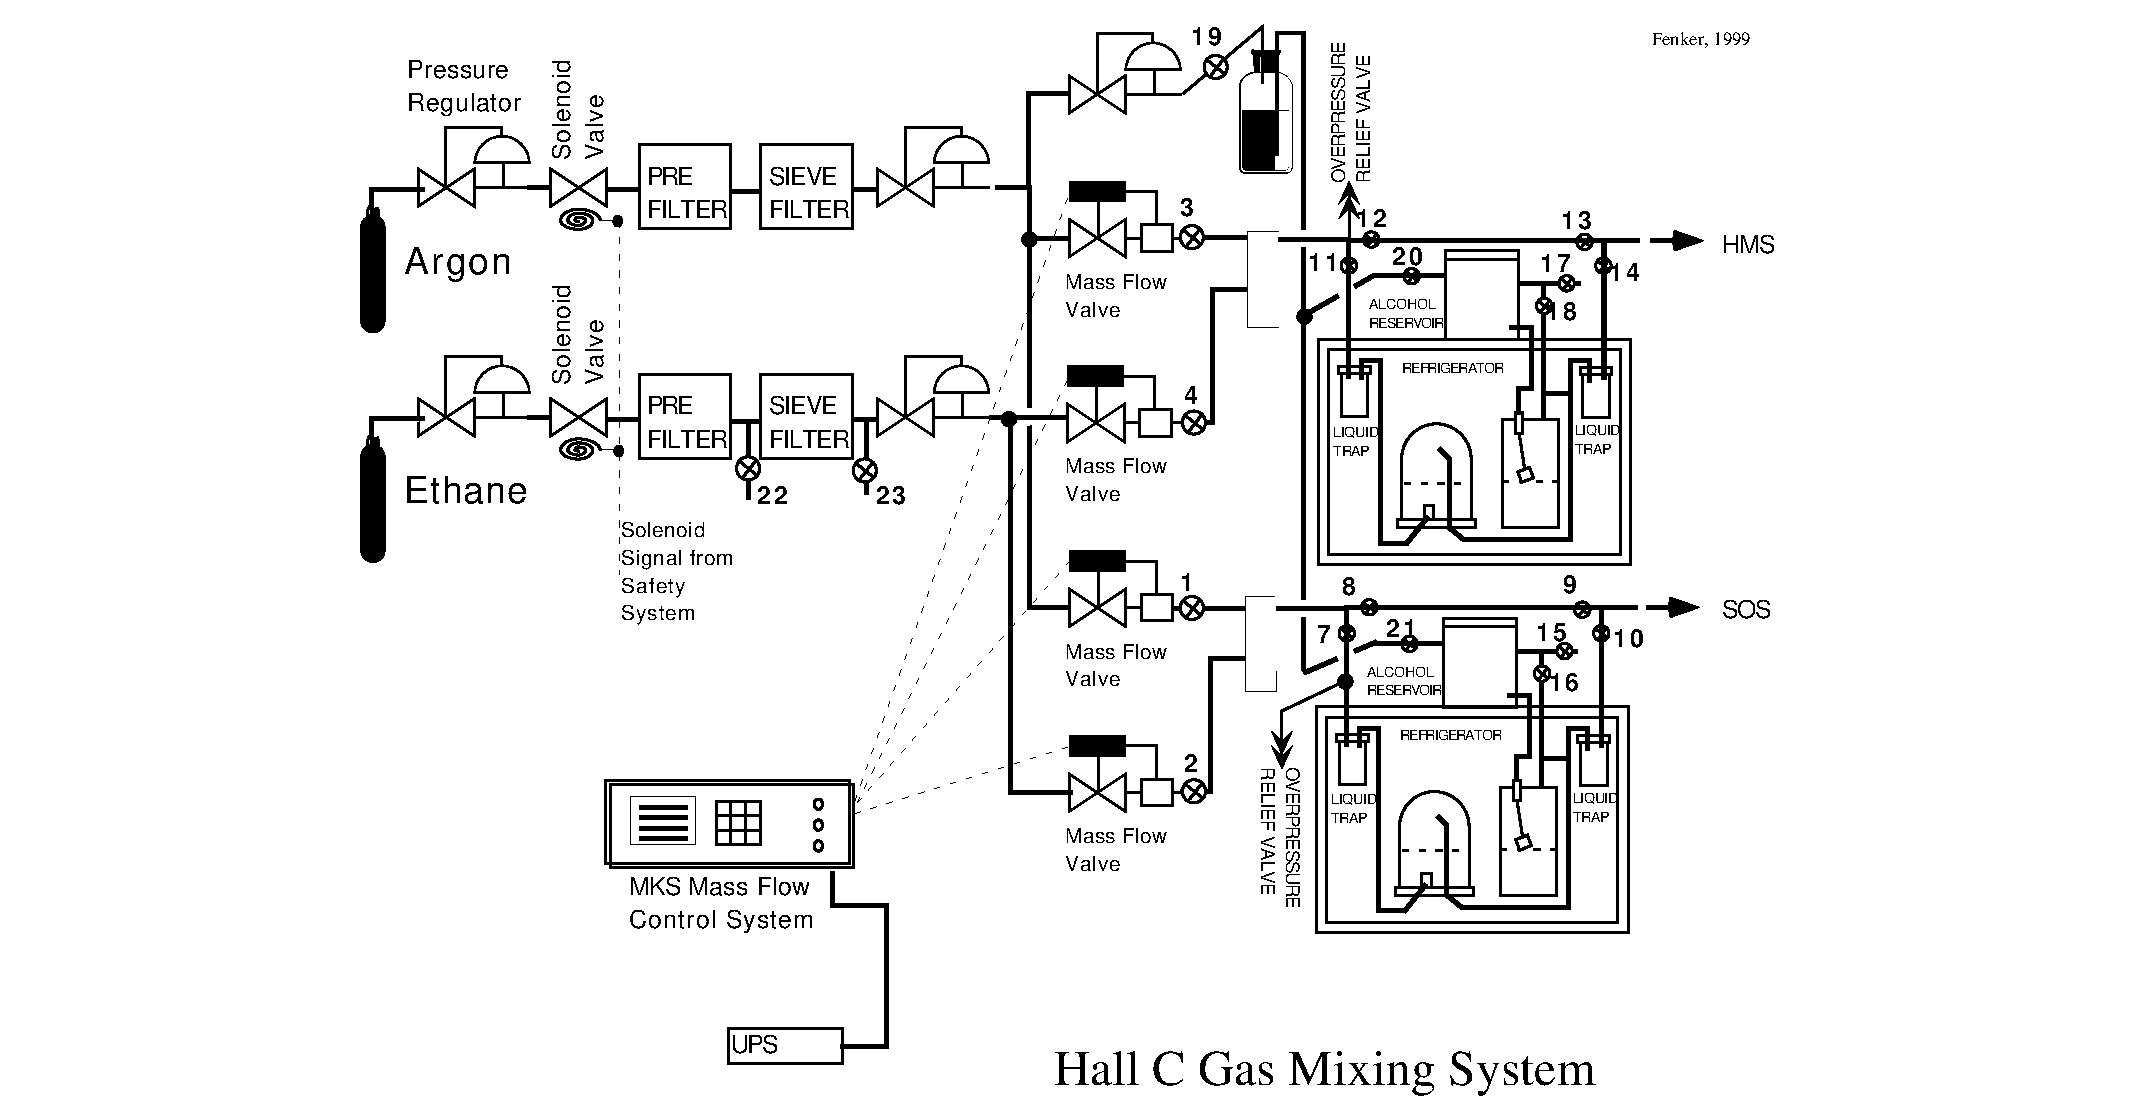
\includegraphics[width=6in,bb=12 12 750 590]{detectors/HallCGasMixlvl1.eps}
\caption{Diagram of Hall~C Gas Mixing System\label{fig:gas_mix}}
\end{figure}

\paragraph{Normal Operation.}

For normal operation, with the alcohol systems in use, the following valves
should be set as follows:

{\bf For The HMS:}

Open - 3, 4, 11, 14; Closed - 12, 13, 17, 18, 19, 20


Unless the gas \#3 Mass flow control valve is installed, valve \#6 should
always be closed.

{\bf For the SOS:}

Open - 1, 2, 7, 10; Closed - 8, 9, 15, 16, 19, 21.


Unless the gas \#3 Mass flow  control valve is installed, valve \#5 should
always be closed.

\paragraph{Operating the MKS 647 Mass Flow Controller.}

The gas flow is controlled by a MKS 647 controller and mass flow
control valves.  The 647 is menu driven from a CRT in the front panel and
with a keypad with cursor controls. The 647 features a non-volatile memory
so settings are retained even if the unit is unpowered.  The initial menu
upon startup is the Command Menu.  For normal operation use either the User
Display menu (Command menu item \#1) or the Extended Display menu (Command
menu item \#2).  The User Display menu shows actual flow in each channel and
the total flow in all channels.  The Extended Display menu shows actual
flow, flow set point, units, valve full scale range, gas calibration
factor, whether that channel is enabled, and whether each channel is
operating in master, slave, or independent mode.

{\bf To set flow rates:}

The flow rate set points are adjusted from the Extended Display
menu.  There are two methods to change valve flow rate set point.  If you
want to enter a specific value you must first turn off the flow in that
channel or all of the channels.  Using the cursor keys move the cursor to
the desired channel.  Enter the desired flow rate.

The flow rate set point can be changed with gas flowing using the
cursor keys. In the Extended Display mode move the cursor to the desired
channel using the left/right cursor keys.  The set point can then be
adjusted up or down using the cursor up/down keys.

{\bf To turn gas flow on or off:}

The gas flow can be turned on or off while in any menu.  When any
of the mass flow valves are open the green LED labeled ``GAS ON" on the 647
is lit.  When none of the gas flow valves are open the red ``STAND BY" LED
will be flashing.  In the Extended Display menu the bottom line displays on
or off, by channel, to show which mass flow valves are enabled.  The green
LED must be lit and an ``ON" must be displayed in the bottom row of the
Extended Display menu for gas to be flowing in a particular channel.

{\bf Turning the gas on or off is done in two steps which can be done in
either order.}
Each channel must be enabled by pressing ``ON" and then
that channel number.  The command input must be enabled by pressing ``ON"
and then ``ALL" from the keypad.  This allows a single channel or all of the
enabled channels to be turned on or off at once.  Both steps must be
performed initially, but thereafter only one of the steps need be performed
to cycle the gas flow on or off.

To turn gas off in a single channel press ``OFF" and then the
desired channel.  If you want to close all the valves simultaneously, press
the ``OFF" key and then the ``ALL/0" key.  To turn gas back on you must
reverse whichever sequence you used to stop the gas flow.  For example if
you turned the gas off by pressing ``OFF" and then the channel number, it
must be turned back on by pressing ``on" and then the channel number.  If
you turn off all the channels by pressing ``OFF" , ``ALL" you must turn it
back on by pressing ``ON" , ``ALL."

{\bf To by-pass the alcohol system:}

For the HMS:
Open valves 12 \& 13, then close valves 11 \& 14, in that order!

For the SOS:
Open valves 8 \& 9, then close valves 7 \& 10, in that order!

{\bf To refill the alcohol bubblers:}

The alcohol bubbler system features a refill system that allows
filling directly from the bottle, minimizing exposure of the alcohol to air
and reducing the possibility of a spill.
{\bf The reservoirs should be refilled
before they become empty to maintain a head of liquid over the float valve
which will prevent air from entering the system.}
In the back of the gas
system rack is a holder for gallon sized alcohol bottles and a cap with dip
tube.  Place a new bottle in the bottle holder and replace the cap with the
cap with dip tube.

\begin{itemize}
\item{ \bf{Step-by-Step Instructions for Refilling the SOS Alcohol Bubbler}\\
\em{These steps must be individually completed in the order listed!}}\\
Refer to Fig.~\ref{fig:gas_mix}. 
\begin{enumerate}
\item{If needed, install a full bottle of alcohol in the back of the gas racks as mentioned in the preceeding paragraph.}
\item{{\em Open valves 8,9. Close valves 7,10} to Put the SOS alcohol bubbler in BYPASS.}
\item{{\em Close valve 16} to isolate the warm reservoir gas from the bubbler.}
\item{{\em Open valve 15} to bleed off the warm reservoir gas pressure.}
\item{{\em Open valve 19} to pressurize the alcohol bottle.}
\item{{\em Open valve 21} to flow alcohol into the warm reservoir.}
\item{When the alcohol level in the sight-glass is within 2cm of the top, stop
the flow of alcohol: {\em Close valve 21.}}
\item{{\em Close valve 19.}}
\item{{\em Open valve 16.}}
\item{{\em Close valve 15.}}
\item{{\em Open Valves 7 and 10. Close Valves 8 and 9.}}
\item{Record what you did in both the gas logbook and the electronic logbook.} 
\end{enumerate}

\item{ \bf{Step-by-Step Instructions for Refilling the HMS Alcohol Bubbler}\\
\em{These steps must be individually completed in the order listed!}}\\
Refer to Fig.~\ref{fig:gas_mix}. 
\begin{enumerate}
\item{If needed, install a full bottle of alcohol in the back of the gas racks as mentioned in the preceeding paragraph.}
\item{ {\em Open valves 12,13. Close valves 11,14} to Put the HMS alcohol bubbler in BYPASS.}
\item{{\em Close valve 18} to isolate the warm reservoir gas from the bubbler.}
\item{{\em Open valve 17} to bleed off the warm reservoir gas pressure.}
\item{{\em Open valve 19} to pressurize the alcohol bottle.}
\item{{\em Open valve 20} to flow alcohol into the warm reservoir.}
\item{When the alcohol level in the sight-glass is within 2cm of the top, stop
the flow of alcohol: {\em Close valve 20.}}
\item{{\em Close valve 19.}}
\item{{\em Open valve 18.}}
\item{{\em Close valve 17.}}
\item{{\em Open Valves 11 and 14. Close Valves 12 and 13.}}
\item{Record what you did in both the gas logbook and the electronic logbook.} 
\end{enumerate}
\end{itemize}

\paragraph{Recalibration and Rezeroing}

Mass flow control valves(the 2259c's) require periodic recalibration
and rezeroing.

\noindent{\bf Rezeroing:}

Rezeroing or Zero Offset is easy and can be performed often and should be
performed every time the unit is moved, recalibrated, or adjusted.  The
valve must be in the orientation it will be used to rezero it.
{\bf To use the
Auto Zero function one must insure that the channel is not switched on and
there is no possibility of flow in that channel ie. the manual valve in
line with the mass flow valve must be closed.}
The Zero Adjust menu is
reached from the main menu to the Instrument Setup menu.  In the Zero
Adjust menu move the cursor to the word EXEC on the channel to be zeroed in
Zero Adjust line.  The unit will measure the current value and use that for
the new zero offset.  If the operation is successful the word EXEC will be
changed to Done.  If the offset is too large or that channel is on, the
unit will display fail.  In that case, one should check if there is any
flow (even extremely small flow) through the valve.

\noindent{\bf Recalibration:}

MKS recommends recalibration every 12-24 months.  The valves must be
returned to the factory for recalibration.  After reinstallation, the
valves need to be rezeroed.

\paragraph{Filtering}

{\bf All filter maintenance should be performed with the gas supplies shut off
at the tanks.  Insure that no pressure remains inside the filter
before proceeding.}

Both input channels of this system feature high performance long life
filters using a pre-filter and molecular sieve in stainless steel filter
vessels.  The pre-filter and filter cartridges are available from the
company listed below.  The pre-filter is a mechanical filter to remove
liquids and solids from the gas stream and to protect the molecular sieve
downstream from it.

\noindent{\bf Replacing filter cartridges:}

The cartridges are replaced by loosening the nut on the bottom of the bowl
and removing the bowl.  The cartridges can be exchanged and the bowl and
nut replaced and tightened.

\noindent{\bf Using 13x molecular sieve filters with ethane:}

{\sl It has been reported that when using 13x molecular sieve filters with
ethane, some ethane is trapped in the filter making the cartridges
flammable.   To purge the ethane from the  filter cartridge a pair valves
and external connections are on either side of that cartridge.  A nitrogen
line should be connected to valve \#22 and a vent line connected to valve
\#23 before changing filters. Nitrogen should flow through the filter for
several hours before changing.}

\noindent {\bf Purchasing Filters and Repairs:}

The following filter types are used:
\begin{itemize}
\item[~]3/100-12-bx microfiber pre-filter
\item[~]CI-100-12-103 molecular sieve final filter
\end{itemize}

These filter cartridges are available from:  Balston Filters, 6767 Forest Hills Drive, Suite 305, Richmond, VA 23225,  1-800-221-1900

Recalibration and repair of the mass flow control valves and controller are
available from:  MKS instruments, Six Shattuck Road, Andover, MA 01810,  
1-800-227-8766 or508-975-2350



\subsection{Hall C Laser Pulser System}
The Hall C laser pulser sytem provides light pulses
in the visible  blue scintillation region to monitor
the gain stability of the HMS and SOS shower counters and scintillators,
and, at a later stage, the neutron detector of the $G_{En}$ experiment.

\paragraph{UV Laser System}
We use a nitrogen Laser that provides UV laser pulses at 337 nm
from 1 to 50 Hz repetition rate. The output power is 250 $\mu$J.
It is located in a designated area in the Counting House of Hall C.
The laser is enclosed in an aluminum box where the laser light is directed
onto a scintillation fiber after passing through two optical filters
to optimize the light output. 
The laser light is absorbed in the scintillation fiber
and converted to visible blue scintillation light. Both ends of the
scintillation fiber are coupled using CT connectors, mounted on an
aluminum casing, to regular
1 mm diameter multimode plastic optical fibers. One fiber output is
connected to a PIN diode to monitor the light output; the other
fiber is brought downstairs into Hall C where it is connected to 
a distribution box (1:24) located in the cupboard below the pivot. From
this distribution box 4 fibers are running to the HMS spectrometer and
4 to the SOS spectrometer, where they
are connected again to distribution boxes (1:64). The individual
outputs of the final distribution box are connected to the scintillators
and lead glass shower counters. The light pulses in the detector
produce a trigger in the data acquisition system and ADC and TDC
information is read out. Normalizing the peak positions of the light 
pulses to the PIN diode ADC value is a tool to monitor the gain of
each photo multiplier tube throughout the experiments.

\paragraph{Laser Operation} 
In order to turn on the nitrogen laser the right half of the top
plate of the aluminum box needs to be removed. Inside the box 
the laser and the optics is mounted on a single aluminum board.
The lasing part of the laser is confined in the left part of the box
with a separation in the central region of the box. Due to this separation
no UV laser light can escape from this left part of the box,
even during operation, so that the user can safely remove and install the
top plate above the right half of the laser casing.
The laser itself has a security key that needs 
to be in a vertical position when the power switch is pressed. After
2 minutes of warmup-time an orange light turns on indicating that
it is possible now to turn the key into its horizontal position.
After this it takes 15 seconds until the laser actually turns on.
In the event of a power failure the laser will turn off and will not
turn on again after power is restored. It is necessary to turn the key
back to its vertical position and to reset the safety system of the laser.
The laser can now be turned on again by switching the key back to its
horizontal position. The pulse frequency of the laser can be regulated by
turning the black knob at the rear of the laser casing.

\section{The HMS Detector Package and Shield House }

All the detectors are in the shield house (also referred to as the detector hut,
located at the top of the
rear set of stairs). The shield house has one wall which is removable
in order to gain completely free access to the detectors. The removal
of this wall is rarely needed as there is a door that provides access
to the hut and there is adequate room inside the hut for most activities.
Essentially, the only activities that require the removal of the hut
wall are the installation or removal of an entire detector. The
hut wall may only be removed by Hall~C approved, and trained crane
operators and requires
several people. Mike Fowler, Hall~C mechanical technician,  
must be contacted if the hut wall needs to be removed.

The hut door is motorized, and must therefore be opened manually. Keep in mind when opening and closing the
shield house door that it weighs approximately 15 tons and therefore has
considerable inertia. This means that you must pull backwards on the door
in order to slow it down near the end of its desired motion.

The detector package is key to a successful measurement. Its
proper operation should therefore be constantly monitored during shifts. There
are normally a number of diagnostic spectra available to aid in this
process.  Typically each collaboration customizes it's own set of
diagnostic spectra.  

\subsection{High Voltage Supplies}

All the detector elements require the use of High Voltage. The
high voltage supplies for the detectors are located in the
electronics room of the counting house. They are connected to
the detectorsshield house through a multiconductor high voltage patch system,
and to the detectors through coaxial cables with SHV connectors.
During experiments the control of the high voltage supplies is
done remotely via computer and a display is available on one 
of the xterms around the console in the Hall~C counting house. The control is via
EPICS and includes a graphical display so that the status of each
HV channel can be seen at a glance. See section~\ref{par:hv_ops} for
operating instructions.

As a general rule no work should be done on detectors which are under
High Voltage and
High Voltage cables should never be removed or installed while the supply is on.
General information about the use of the {\em CAEN} power supplies can be
found in a previous Section.


\subsection{Drift Chambers}

\paragraph{Overview}

The drift chambers provide accurate measurements of the particles
position and angles in the detector hut. This information can be combined
with a knowledge of the spectrometer optics to infer the trajectory of the
particles at the target.

The planes are designated X,Y,U,V,Y$'$, and X$'$.
X and X$'$ wires measure position along the dispersive direction.
Y and Y$'$ wires measure in the transverse direction while
the U and V planes are inclined at fifteen degrees with respect to the
X planes.

In addition to High Voltage the drift chambers have amplifier discriminator
cards which require Low Voltage. These Low Voltage supplies
(built by {\em Accopian}) are
in racks in the shield house. They are not computer controlled.

The thresholds of the discriminators are held by a third set of supplies
which are located upstairs in the counting house. This control
is in the left side of the far left hand set of blue racks (near the disk drives) in the
electronics bay of the Hall~C counting house.

The amplified and discriminated signals from the chambers are fed
to the starts of {\em LeCroy} Model 1877 Fastbus pipeline TDC's. These
TDC's are located in the detector hut in an electronics rack on the
far side (from the door) of the detector mounting stand.
%The hazards associated with electronics crates are discussed in
%\cite{bi:arr95}.

The chambers are filled with a mixture of Argon, Ethane and Isopropyl Alcohol
($\approx$ 49.5 $\%$, 49.5 $\%$  and $1\%$ by weight respectively).
The gas bottles are in the bottle racks behind the gas shed. The gas shed
is located in the parking lot to the left of the counting house when one is facing the counting
house between the counting house and the accelerator
service building.  The alcohol is placed in the gas
by bubbling the gas through a refrigerated bubbler. This bubbler is
located in the gas shed.

There are gas log books that must be completed each shift.
When a bottle is near empty it should be changed.
Care should be used when handling high pressure gas bottles as the
potential energy stored in such a bottle is tremendous.
Gas bottles can only be changed by authorized personnel.

The gas mixing system is in the gas shed. The mixing is accomplished
by an electronic system. The flow rates of the gases can be read off the
LCD display of the flow meter located in the gas panel rack in the shed.
This information must be entered in the gas log book along with the bottle contents.
Only authorized personnel should make adjustments to the gas flow system.
All permanent members
of the Hall~C physics and engineering staff may change gas bottles.

As is true for all detector systems, in case you note a loss of power
during experiment conditions, check the VESDA panel in the Hall~C counting
house to see whether there is a potential fire before resetting (also
see the section on ``Fire" at the beginning of this chapter).

\paragraph {Gas Flow Operating Procedures}

The HMS drift chambers use a 50:50 mixture (by weight) of argon and
ethane gas.  Each chamber has a volume of about 120 liters.  Each is
operated slightly above atmospheric pressure.  The gas flow through
the two chambers can be varied and is typically set at 1000 cc/min
when flushing (full purge in about 2.5 hours) and 400 cc/min when operating
at low to moderate charged particle rates.  The chambers are connected
in parallel for gas flow as shown in Figure~\ref{fig:5.1}.  There are flow meters 
connected
to the exit line of each chamber.  The gas flow control electronics
and gas handling system (GHS) are located in the gas shed just outside
of the Hall~C counting house.  The gas cylinders are kept just outside of
this shed.  Both the argon and ethane cylinders have regulators (the ethane
cylinder must use a CGA-350 regulator since it is a combustible gas) for
reading the gas pressure in the bottle (high pressure) and in the line (low
pressure).  However, the ethane
in the cylinder is a liquid, so that the WEIGHT of the cylinder is important
for monitoring the amount of ethane remaining.  The ethane
cylinder sits on a 'bathroom scale' for this reason.  An empty cylinder
(standard size) weighs 110 lbs.

\begin{figure}
\includegraphics[height=7.5in]{detectors/HMSdriftch.ps}
\caption{The Gas Handling System for the HMS Drift Chambers. \label{fig:5.1}}
\end{figure}

\begin{center}
{\bf Procedure}
\end{center}

\begin{enumerate}
\item {Visually check that the gas flow lines are connected to the two
HMS chambers.}
\item {Check gas pressure and amount in gas cylinders (Ar and C$_2$H$_6$).}
\item {Turn on the gas flow on the MKS controller in the gas hut.}
\item {Set flow through channels three and four to 800 sccm each
(for purging).}
\item {After about 15 minutes, the oil bubbler in the gas hut should
indicate flow.}
\item {The flow rates as read on the flow meters at the chambers should
indicate very low flow (0.3 or so).}
\end{enumerate}

The above settings are for 400 sccm flow through each chamber.  The gas
cylinders should be changed when about 90\% used.  The gas handling system
parameters should be checked every shift (see the checklist at the end of
this document).

\paragraph{Electronics Operating Procedures}

The readout electronics associated with the HMS drift chambers are all
commercial products from LeCroy Research Systems, Nanometrics, Kinetic Systems,
and BiRa Corporation.  There are 544 electronics channels per chamber for
a total of 1088 readout channels.  These anodes are read out using LRS 2735DC
and Nanometrics N-277 preamplifier/discriminator cards mounted directly
on the chambers.  Each chamber has both types of cards, however each plane
(of six total planes per chamber) has only one type of card.  The
digitized signals are sent to FASTBUS TDC inside of the detector hut
via twisted pair cable.  The low voltage (preamplifier) power supplies
(the Acopian supplies)
are in the 13 inch blue rack at the rear of the detector hut.  The
threshold voltage power supplies are on the frame under the Cerenkov
counter.  The remote
threshold power supplies are located in the electronics room of the counting
house.

\begin{center}
{\bf Procedure (in the detector hut)}
\end{center}

\begin{enumerate}
\item {Turn on low voltage power supplies (the Acopian Supplies).}
\item {Turn on threshold voltage power supply to appropriate setting.}
\item {Turn on the FASTBUS power supply if it is not already on.}
\end{enumerate}

It is important that the Acopian power supplies be turned on {\bf BEFORE} the
FASTBUS supplies or the FASTBUS crate will hang up.  The threshold voltage
can be controlled locally in the detector hut or remotely in the
counting house. There is approximately a one volt drop in the threshold
voltage line in going from upstairs in the counting house to
downstairs in the detector hut.  Hence the supplies in the counting
house should be set to 5.5 volts. The local/remote switch is on the
controller in the
detector hut.  It should be switched to remote before exiting the hut.  The
LeCroy preamp/disc cards have LEDs (a green and a red light) which indicate
that the power is delivered properly to the chamber electronics.

\paragraph{High Voltage Operating Procedures}

Only formally authorized person may alter drift chamber high voltage.
There are four different voltages per chamber which must be turned on at the
proper time and monitored throughout the experiment.  {\bf MAKE SURE THAT
GAS IS FLOWING THROUGH THE CHAMBERS AND THAT THERE ARE 
EDGE 
CARDS MOUNTED
ON ALL READOUT CHANNELS BEFORE TURNING ON HIGH VOLTAGE.}  
The high voltage
power supplies are the CAEN supplies located in relay rack CH03B17 in
the counting house electronics room.  The
voltages are set remotely using the GUI in the counting
house. See section \ref{par:hv_ops} for operating instructions.
The four different voltages are (nominally): triangle
wires (corner field wires) (-2500 V),
square wires (-2250 V), circle wires (-1800 V), and guard wires (-1500 V).
Note that each HMS drift chamber {\em plane} has its own triangle, circle,
and square voltage source, while there is only one guard wire voltage
source per {\em chamber}.
\begin{center}
{\bf Procedure (in the detector hut)}
\end{center}

\begin{enumerate}
\item {Make sure a 2735DC card or a grounding plate is on each instrumented
connector on the chamber.}
\item {Make sure that there is gas flow, particularly Ar gas.}
\item {Make sure high voltage cables are properly connected to
chamber.}
\item {Turn on high voltage, using the EPICS GUI in the counting house, 
to proper settings.}
\end{enumerate}

The CAEN power supplies, when operated remotely, are controlled by the
EPICS control system.  To operate, log on to vxworks, get the high
voltage monitors (use the rightmost mouse button to bring up the menu)
and choose the chamber voltage group.  Each high voltage channel is
independently controlled.

In general all of the voltages and gas flow should be left on, even when
no data is being collected.  The gas supply should be checked periodically,
approximately once every shift.  The gas bottles' supply is depleted
after about 2 weeks at the nominal (400 cc/min) flow rate.
In the case of a HV trip, try cycling the CAEN power supplies.  If this fails, call
one of the responsible persons listed in the Responsible Personnel Section 
of the \htmladdnormallinkfoot{ESAD}{http://www.jlab.org/Hall-C/document}.




\subsection{Scintillator Hodoscopes (HMS and SOS)}

The purpose of the scintillator hodoscopes is to provide a clean
trigger as well as particle identification by time of flight (TOF). These
detectors consist of two pairs of spatially separated scintillator
layers: a pair comprised of S1X and S1Y, and approximately 2 meters away a pair
comprised of S2X and S2Y. General characteristics of the BC404 scintillator
material are as follows:

\begin{itemize}
\item{Polyvinyltoluene (PVT) is the base material. }
\item{Light output is 68\% that of Anthracene. }
\item{Wavelength of maximum emission is 408 nm.}
\item{Decay constant of the main fluorescence component is 1.8 ns.}
\item{Bulk attenuation length is 160 cm.}
\end{itemize}

	The specific dimensions for the scintillator elements in the HMS
and SOS are found in Table~\ref{tab:tof_scintillators}.
\begin{table}
\caption{Dimensions (at 70~F.) of the scintillators for the HMS TOF system. 
\label{tab:tof_scintillators}}
\begin{center}
  \begin{tabular}{ccccc}
	&Thickness	&Width		&Length		&Number	\\
	&		&		&		&	\\
\hline
X(HMS)	&	1cm	&	8.0cm	&	75.5cm	&32 units\\
Y(HMS)	&	1cm	&	8.0cm	&	120.5cm	&20 units\\
	&		&		&		&	\\
X1(SOS) &       1cm     &       7.5cm   &       36.5cm  &9 units\\
Y1(SOS) &       1cm     &       4.5cm   &       63.5cm  &9 units\\
X2(SOS) &       1cm     &       7.5cm   &       36.5cm  &16 units\\
Y2(SOS) &       1cm     &       4.5cm   &       112.5cm &9 units\\
  \end{tabular}
\end{center}
\end{table}
Each scintillator is read out by two Philips XP2282B photomultiplier
tubes (PMT's). These PMT's are 8-stage tubes with nominal operation at
2500 volts. The bases have two anode outputs, one of which is terminated with a
short clip line and 40 Ohms.  Because of pmt to pmt variations in gain and the
5\% precision zener diodes in the bases, the spread in gains can be a factor of
2-3. Individual high voltages must therefore be adjusted to balance the gains.
The gains have been carefully matched with a source, and HV save files exist,
so the gains will not normally need to be readjusted. If gain adjustment is
necessary, inform one of the hodoscope contact persons as soon as possible.
Mysterious gain shifts are probably due to transient problems like bad solder
contacts or broken glue joints. They require repair. A rough rule of thumb is
that an increase of 50 volts will increase the gain by 30\%.

With our base, the HV channel will trip on overcurrent (3 mA) at 2900 V
(this base is essentially divider C in the Philips catalog). If a channel needs
more than 2800 volts, and the base and glue joints are okay, then our policy
is to replace the pmt. We have several spare modules in the counting room.
In desperation, ``spares" can be taken from the edges of the acceptance. In the
HMS, S1X16 or S2X16 contain little or no useful data, and similarly for S1Y01
or S1Y10.

	The light guide material is UVT lucite.  Wrapping material for the SOS scintillator elements was one layer of 
aluminized mylar (aluminum side facing inward), followed by two layers of
tedlar for light tightness. The HMS elements were wrapped in aluminum foil,
followed by one layer of tedlar.

	The SOS hodoscopes are mounted in aluminum frames, with brackets over
the lightguides and holders supporting the elements also at the tube/base
assembly. The SOS y-counters are EXTREMELY delicate at the glue joints
connecting the angled light guide with the flat section, due to the geometry.
The HMS elements are supported at the lightguides. In case of repair use BC-600
glue. Each element has a 1 mm plastic fiber glued into the light guide. These
fibers are also very delicate and care must be taken when moving a scintillator
element to avoid snagging and breaking the fibers.

{\bf What to check}: Before starting to operate the detectors, one has to
check the trip setting (current limit) of the HV power supply for each channel
and the set HV value of each channel. During operation, the current of each
channel and its HV should be periodically checked. The HV should be on for at
least half an hour before taking data. During runs one should check the
histogram of the plane hit distribution. This should be rather flat reflecting
the normal trigger requirement of 3 out of 4 planes. Also the element hit
distributions for the individual planes should be checked regularly. These
distributions are defined for both ends of the elements using both ADC and TDC
information.

{\bf Nomenclature}:
The coordinate system (right handed, following TRANSPORT
convention) is defined as z downstream, x pointing down, and when looking
downstream, y to the left. In this convention the X-tubes at positive Y are
called X+ and the Y tubes at the bottom (pos x ) are called Y+. Numbering of
the elements is done as one would read a book in English: left to right in the
case of the Y and top to bottom in X.

	There are one ADC and one high resolution (25 ps/channel) TDC per PMT.
For the SOS, S1X and S1Y and S2Y each have 18 channels, while S2X has 32 making
it 86 channels in total. Each ``X''plane in the HMS has 32 and each
``Y'' has 20, making it 104 channels in total.

	The signals are carried on an RG-8 size cable which is a Belden 213
equivalent. The nominal specifications are 50 Ohm impedance and the signal
velocity is 0.82c . The signals are passively split in the counting house with
one going to the ADC and one going to leading edge discriminators. The
performance is typically 100 and 150 psec mean time resolution (sigma) per
element for the SOS and HMS, respectively.

\subsection{Gas Cerenkov Detector}

A charged particle travelling faster
than the speed of light in the medium will create an electromagnetic
disturbance in the medium. The radiation emitted by this process is
called Cerenkov radiation after its discoverer.

Cerenkov radiation is conically distributed about the trajectory of the
particle, with an angle given by
$$
	\cos{\theta} = \frac{1}{\beta n}
$$
where the index of refraction $n = c/u$ and $\beta = v/c$, with $c$
the speed of light in vacuum, $u$ the speed of light in the medium,
and $v$ the speed of the particle.

The index of refraction allows one to control the threshold particle velocity 
$v_{T}=u=c/n$ below which there is no Cerenkov light produced, and above which there 
is Cerenkov light produced.  For a gas, the quantity $n-1$ is proportional to the pressure, 
so adjusting the pressure of the gas allows one to select the
threshold velocity. Adjusting the threshold velocity actually allows one to select particles of
different mass.  Given the same momentum, two particles of different mass
will have different velocity.  Therefore, a Cerenkov detector can be tuned,
for instance, to distinguish electrons from pions.

	The HMS Cerenkov detector consists of a large cylindrical
tank, $\phi_{in} = 59"$, $L = 60"$, containing two mirrors which focus
light onto two 5 inch Burle 8854 multiplier photo  tubes (PMT's). The tank
has been installed with 0.04 inch thick 2024-T3 Aluminum windows
covering the circular ends of the cylindrical tank. These
windows were hydrostatically formed (and hence tested) at a pressure
of 28 PSI. The tank itself was helium leak checked and is leak free
on a scale of 10$^{-8}$ Atm-cm$^3$/s. In addition, the tank was hydrostatically
tested at a pressure of 35 PSI. Detailed information on this testing
program can be found in \cite {bi:tank}, \cite {bi:wind}.

The tank is mounted on the detector rails using a three point
alignment scheme. The rails are easily capable of supporting the
weight of the tank without deformation.  
The gas handling system for the tank
is designed to enable the tank to be filled with
pure gas, CO2 or N$_2$, at the desired operating
pressure which is, $\approx$ 1 Atm (11.5 PSI) for the near future.

The system consists of the fill gas bottle and primary
pressure regulator which are in a bottle rack that's welded to
the bottom of the HMS detector hut on the small angle side at a height
of about six inches from the hall floor. The primary regulator is
a Matheson model 2596 with a maximum outlet pressure of 400 PSI.
During fills this regulator should be set to 150 PSI.
The outlet of this pressure regulator is connected to the
main gas control panel which is mounted on the first floor balcony
of the detector hut behind the dipole control racks. All connecting
tubes in the system are 0.25 inch diameter stainless steel tubing with
the exception of the nitrogen purge line which is thick wall tygon.
At the entrance to the gas panel there is a 0-300 PSI gauge so that
the pressure in the inlet line can be viewed by the operator.
The line is then relieved by a Circle Seal relief valve set at 200 PSI.
After this, the gas passes through a second regulator (Matheson 3420)
which has an
outlet pressure range of 0-60 PSI. This regulator can be set at
up to 40 PSI for high flow during the early stages of fills
(the line is relieved further downstream by a second
Circle Seal relief valve set at 45 PSI) and then reduced as
the desired operating pressure is approached. Following the second regulator
and its relief valve the gas passes through oil and oxygen filters.
A 120 Volt AC solenoid valve (ASCO) switched with a solid state
relay is used to isolate the gas flow from the tank. The state of
the relay and hence the valve is indicated by a LED on the panel.
The gas line is routed through an opening in the floor of the detector hut
to the tank inlet. A gauge on the panel allows the operator to view
the pressure in the inlet line (the same as the tank pressure
when the subsequent manual valve is open, see following).
At the inlet there is a pair of manual valves (NUPRO)
which allow the fill line to be purged.
During operation the valve which vents the
line to atmosphere is closed and the valve to the tank inlet is open.
The tank is relieved by a 1 inch diameter, 1 PSI pop off (NUPRO) which was
sized to take the
maximum flow of the second regulator even if that regulator has failed
wide open. There is a pressure gauge on the tank so that its condition
can be determined by workers in the shield house. In addition,
there is a Omega pressure transducer (PX-305-05A) and a temperature
transducer attached to the tank. These are read out and powered by
units (Omega) which are located below the gas panel.  Outputs of these
are currently viewed with a video camera attached
to a monitor in the counting house.

Before filling, the tank is first cleaned by executing several pump
and purge cycles. The pump that is used to evacuate the tank is located on a
platform welded to the small angle side of the shield house balcony
which can be accessed from the small angle side of the HMS carriage.
Eventually, it will be possible to switch the power for this pump
from the gas control panel with a relay but currently it
is necessary to turn the pump on and off with a switch located on the pump.
The low pressure side of this pump is equipped with a liquid nitrogen
cold trap to prevent any contamination of the tank (or mirrors !)
with pump oil. This trap will remain filled for approximately
12 hours and should always be checked before use. There is currently
a manual valve located at the Cerenkov tank that isolates the tank from
the pump.  This valve will later be replaced by a pneumatically actuated
solenoid valve that will be controlled from the gas panel.
There is a manual valve on the tank which is equipped with a hose
barb through which clean nitrogen purge gas can be admitted to the tank.
The nitrogen gas comes from a spigot on the HMS cryogenic handling system
located along the upper catwalk of the HMS. The nitrogen system
delivers gas at a line pressure of $\approx$ 40 PSI (this pressure can
be read on a gauge at the pivot end of the catwalk). The flow
rate is readable from a flow meter attached to the spigot. A flow of
about 150 - 200 cfm is reasonable. The tank should not be filled to
more than -5 in Hg during purge cycles.

The tank contains two 5 inch PMT's which use {\bf positive} HV.
Note that all the other PMT bases in the HMS are designed for use with
negative HV. They operate
at between 2000 and 2700 Volts. The Anode is at HV and its signal is
viewed through a decoupling capacitor in the base. The HV is supplied
by one pod of the same {\em CAEN} power supply used for the drift chambers.

The mirrors in the tank may require adjustment for optimal focusing
on the PMT faces. The ports which hold the PMT's are sized big enough to allow
a person inside the tank to make these adjustments. The tank is a confined
space and hence this activity represents an ODH hazard. Stickers indicating
this have been placed on the PMT ports. Before an entry into the tank the
atmosphere in the interior must be surveyed by a member of the physics
division EH$\&$S staff.
This adjustment should only
be done by personnel who understand the fiducial markings of the PMT
mounting system. The interior of the tank has foot braces and hand holds welded
to allow this work at the angle of the detector rails.

\paragraph{Operation Procedures}

\begin{figure}
%\GHS
\includegraphics[height=5in,width=6in]{detectors/HMSgasC.ps}
\caption{The Gas Handling System for the HMS \Cerenkov\ Detector. \label{fig:gas}}
\end{figure}

The HMS \Cerenkov\ Detector operates either as an e/$\pi$ or $\pi$/p
discriminator. Each mode has a unique set of procedures to prepare the tank
for operation. The nomenclature used in the description of these operation
procedures refers to Figure~\ref{fig:gas}, showing the gas handling system. Components 
shown
inside the dashed box of Figure~\ref{fig:gas}, are all located on the Gas Control Panel.

\paragraph{e/$\bf{\pi}$ Procedures}
For both e/$\bf{\pi}$ and p/$\bf{\pi}$ separation, the procedure 
has been to run with 0.4 to
0.9 (?) atmospheres of C4F10.  This is just a small modifiction to the
current p/pi procedures write-up described in the next section,
with the HMS running sub-atmospheric instead of supra-atmospheric. 

e/$\bf{\pi}$ running can also be accomplished using a nitrogen fill.
This mode of operation requires the tank to be filled with approximately
13.5~psia of $\rm{N_2}$.  The boiloff from the spectrometer magnets is a
perfect source of clean, dry Nitrogen, and is normally used to fill the
\Cerenkov\ tank.

Because the operating pressure is slightly subatmospheric, a pump and fill
procedure is employed.  First make sure that:
\begin{itemize}
\item The 40~mil windows are installed and oriented such that they curve
towards the interior of the tank.
\item Valves {\bf V1-V6} are closed.
\item The LN2 trap is filled.
\item There is enough oil in the pump.
\end{itemize}
The tank is now ready to be evacuated.
\begin{itemize}
\item Turn on the pump.
\item Slowly open {\bf V5}.  This evacuates the pump line.
\item Very slowly open {\bf V4}.  Since this valve connects the pump line to
the detector volume, the pump will work very hard.  Meter this valve
so that the pump is never under extreme stress.  It will take approximately
20~minutes to pump down the tank.
\end{itemize}
The tank can now be filled.
\begin{itemize}
\item Locate the boiloff manifold on the walkway on the top level of the
spectrometer, at the gap between Q3 and the dipole.
\item Turn the valve on this manifold open slightly so that the flow meter
barely registers a flow.
\item Connect the remaining end of the Tygon tubing to the vent of valve
{\bf V3} with a hose clamp.
\item Open valve {\bf V3}.
\item Increase the flow on the flow meter.  Do not exceed 100~cfpm.
\item When {\bf G3} or {\bf EPG} reach the operating pressure, close
the manifold valve.
\item Close {\bf V3}.
\end{itemize}
The fill should take approximately 30 minutes.  The detector should NEVER
be left unattended during a fill.  Frequently check the pressure in the tank
and be aware when the pressure nears one atmosphere.  DO NOT let the pressure
exceed one atmosphere under any circumstances; doing so risks damage to all of
the equipment and personnel in the detector hut.  This pump/fill procedure is usually 
repeated at least once to insure the
purity of the gas.

\paragraph{$\bf{\pi}$/p Procedures}
This mode of operation typically requires the tank to be filled with Freon-12
at pressures varying from 2 to 3~atm.  Because these operating pressures are
greater than 1~atm, the detector must be filled by dilution.  Contamination
from air, however, is not a major problem as the optical absorption properties
of air are actually more favorable than those of Freon-12 itself; the only
difficulty is the increase in pressure needed for a mixture of air and Freon
to achieve the same pion momentum threshold as for a pure sample of Freon.

First prepare the gas handling system:
\begin{itemize}
\item Make sure that the 60~mil windows are installed and oriented such that
they bulge outwards from interior of the tank.
\item Close the valves {\bf V2-V4}, and the valve on regulator {\bf R1}.
{\bf V1}, {\bf SV1}, and the valve on regulator {\bf R2} should be
open.
\item Open the valve on the gas supply bottle.
\item Adjust {\bf R1} to approximately 60 psig.
\item Open the valve on {\bf R1}.
\item Check to make sure gauge {\bf G1} agrees with the pressure setting
on {\bf R1}.
\item Adjust {\bf R2} so that a small flow is detected out the vent of
{\bf V1}.
\item Close {\bf V1}.
\item Adjust {\bf R2} to regulate at the required operating pressure.
\end{itemize}
The tank is now ready for the dilution process.  These steps should be
repeated as few times as possible to minimize the quantity of Freon-12 emitted
to the atmosphere.
\begin{itemize}
\item Record the tank pressure.
\item Open valve {\bf V2}.
\item Monitor the gas pressure until it reaches the required operating pressure.
NEVER let the pressure in the detector exceed 3~atmospheres.
\item Record the final pressure.
\item Open {\bf V3} to vent the tank.
\end{itemize}
From the recorded pressure readings, the threshold momentum of the mixture
of air and Freon-12 can be calculated (assuming the volume of the tank is
fixed).



\subsection{Lead Glass Shower Calorimeter}

The lead glass shower calorimeter consists of four stacks of
TF1 leaded glass (similar to SF1). Each stack contains thirteen
blocks for a total of 52 blocks. The blocks are 10 cm by 10 cm by 70
cm and all are read out by a PMT at one end at least.  Currently the
two layers have PMT readout at both ends.

High energy particles
emit Cerenkov radiation when passing through the glass and a signal
is collected that is proportional to the sum of the path lengths
travelled by all the
particles which are above the threshold for Cerenkov emission. High energy
electrons will produce a large signal as they have a large bremsstralung
cross section and the photons which are produced in the bremsstralung
process have a large cross section to produce electron positron pairs
(all of which will be above the Cerenkov threshold). This process
of bremsstralung followed by pair production is called an electromagnetic
shower.

The histograms associated with the calorimeter should be inspected
regularly to assure that it is functioning properly.


\section{SOS Detector Package and Shield House }

The detector package is the key to a successful experiment. Its proper
operation should be continuously monitored during the experiments.
There are a large number of diagnostic type spectra available to aid in
this monitoring.
All the detectors are in the shield house (also referred to as detector hut).
The (concrete) shield house protects the detectors from the typical large
background environment associated with a high energy electron beam
traversing through materials (target, exit windows, possible scraping, dump).

\subsection{Shield House and Shield House Door}

The shield house interior access is covered by a two piece door. The two
halves counterweight against each other, opening vertically. The bottom
door (30 tons) is 5 tons heavier that the top door. Thus, the door will want
to open naturally if unconstrained. The door control system is used to keep
the doors closed.

The valves in the control system are set by a PLC that resides in a box
mounted beneath the stairs at the rear of the spectrometer. The front panel
of this box has two buttons for control of the door (Open \& Close),
switches for main power \& the two pumps, and several status lights. The
status lights indicate when it is necessary to clean one of the several oil
filters. The door is designed to operate electronically via a control box
mounted along the walkway near the door or from the panel beneath the
stairs. Indicator lights in the various buttons on the control box
illuminate to show the current status.

\begin{description}
\item{\bf Open} Opens the door, electronically activating the hydraulics.
Pressing this switch will illuminate both buttons on the operator panel and
on the
control box. The door will require about 60 seconds to open.
\item{\bf Close} Closes the door, electronically activating the hydraulics.
Pressing this switch will illuminate both buttons on the operator panel and on
the control box. The door will require 60 seconds to close.
\item{\bf Emergency Open} Used only if the hydraulic system fails but electrical
power is available. (i.e. hydraulic pump failure) This button operates
valves so that hydraulic fluid slowly exits the door cylinders and allows the
doors to open. Opening the door this way may require several minutes.
This switch is not spring loaded and will have to be manually reset before
other operations can continue.
\item{\bf Emergency Stop} Stops the movement of the door regardless of
direction.
This switch is not spring loaded and will have to be manually reset before
other operations can continue. Resetting the switch does not resume door
motion. Another button must be pressed to start movement again.
\item{\bf Standby} Once the door is stopped, standby may be used to keep
the door
within 0.5" of its' present position. This switch is disabled during door
movement. If the doors creep through fluid leaking by the seals in the
cylinders while the system is in standby mode the pumps will activate and the
slippage will be corrected. The cleaner the system and newer the cylinder
seals the less this slippage will occur.
\end{description}

The circuit for the door controls is located in boxes C-UPH3 (pumps, circuits
20,22,24) and C-UPL3 (120V, circuit 35).

The control panel controls:

\begin{description}
\item{\bf Open} Same as above.
\item{\bf Close} Same as above.
\item{\bf Large Grey power switch} Switches on power to electronics and pumps.
\item{\bf Pump 1, Pump 2} Each pump may be enabled individually. These two
switched do not start the hydraulic pumps.
\item{\bf On} Starts the enabled hydraulic pumps.
\item{\bf Off} Stops the enabled hydraulic pumps.
\end{description}

\subsection{Opening/Closing SOS Shield House Doors}

To open SOS shield house doors, first confirm appropriate breakers in
breaker panels on right side of carriage are "on". Open doors on power
panel at right rear of carriage, then close right hand door, making sure
that switch handle on outside of door engages switch shaft. Leave left door
open.
Operate switch handle to turn on 480 volt power. Watch message panel on
orange plc box near left end of top row of modules. Message panel should be
blank. If any message appears, {\bf STOP} and call/page Hickson or
Vulcan.  If panel is
blank, proceed. On exterior of right hand door, select either pump \#1 or
pump \#2, then press green "on" button below pump selector switches. Note
sound of pump. Go up S.O.S. stairs to walkway in front of doors. Insert
enable key in control box, and turn to "on" position. Press and hold "open"
button. Button must be depressed for - 5 minutes, 40 seconds to open doors
completely. While opening doors, watch door hydraulic cylinders; cylinder
movement should be synchronized. lf differential movement is observed,
release "open" button, hit "emergency stop'' button and call/page as 
above.  Doors will stop automatically at full open position.
If doors will be open for more than a few minutes, return to floor level
power panel and turn pump off with red "off' button below pump selector
switches, then turn off 480 volt power with switch on exterior of right
hand door. If pump is left on, close doors by pressing and holding "close"
button for - 5 minutes, 40 seconds. Doors will stop automatically when
fully closed.  When doors are closed, turn enable key to "off' and remove
key from control box. Return to 480 volt panel, turn off pump, and turn off
480 volt power. If 480 volt power was turned off while doors remained open
for an extended period, 480 volt power must be turned on to close the doors
as described above. Always observe message panel on plc after turning on
480 volt power. Never proceed If any message is displayed.

NEVER LEAVE 480 VOLT POWER ON DURING BEAM PERMIT.

NEVER USE "STANDBY" MODE.



\paragraph{Safety Items}

With the loss of electrical power all valves close automatically. This will
stop all movement of the door. The fluid in the cylinders may slowly leak
past the seals causing the door to open.

A section of handrail will be (is) attached to the downstream end of the
flip-down section of walkway. This handrail will block access to the doors
until the doors open completely and the flip-down walkway can be rotated
over the lower door.

The toe kick around the roof of the shield house will be (has been)
extended to 8", and sealed to contain fluids in the event of a catastrophic
hydraulic leak. The enclosure should capture 330 gallons of fluid adequate
to contain a complete system rupture.  The most common mode of fluid
loss is a slow drip at a joint. Rupture of a hose, while very unlikely, can
result in loss of fluid in that hose. Pressure indicators in the system
will stop
the system if loss of pressure is detected. See the hydraulic diagram for
the location of the pressure indicators (Figure~\ref{fig:SOSdoorHydSym}: explanation of symbols,
and Figure~\ref{fig:SOSdoorHydDiag}: the hydraulic diagram).

Filter replacement is required when the maintenance light on the control
panel is illuminated. The filter elements are placed between two isolation
valves. The two valves must be closed, and the pressure released before
the filter cover is removed. The filter cover is a screw on/off type. The
elements are not disposable and are designed to be cleaned and replaced.

\subparagraph{Filter Removal}

\begin{enumerate}
\item{Turn off the power to the control system.}
\item{Close the valves on either side of the filter to be replaced.}
\item{Release any built up pressure in the filter and neighboring pipe by
opening the pressure relief needle valve at the filter. Be careful of any fluid
released through the valve. {\sl The released fluid should be captured and
disposed of properly.}}
\item{Unscrew the filter cover.}
\item{Service the filter.}
\item{Replace the filter and cover.}
\item{Close the pressure relief needle valve.}
\item{Open the valves on either side of the filter.}
\end{enumerate}

\subparagraph{Valve Failure}

The solenoid valves have lifetimes of many thousands of cycles.
In a valve fails, the two pressure indicators will start to differ, soon
resulting in a too large difference between the two decoders (one for each
side of the door), causing the motion mechanism to stop.

\subparagraph{Cylinder Failure}

In the unlikely event of a cylinder failure, the door will slip slightly to one
side in the track and any motion will stop.

\paragraph{Manual Door Operation}

In the event that electrical power is lost (and thus hydraulic control) the
door can be opened manually. There are five manual popet valves, that are
to be opened in a certain sequence, that will allow hydraulic fluid to slowly
drain from the cylinders thus opening the doors.

\begin{enumerate}
\item{Open the popet valve at the top of each door cylinder (valves SV-C-9
\& SV-C-10) by
pressing the switch on the valve. The valve is located on the downstream
side at the top of each cylinder.}
\item{Open the popet valve at the bottom of each cylinder (valves SV-C-11
\& SV-C-12) in
the same way. The valve is located on the upstream side at the bottom of
each cylinder.}
\item{Finally open the valve (valve SV-C-13) located on the rear wall of the
spectrometer, above the electronics hut.}
\end{enumerate}

The fluid drains from the cylinders slowly. Opening the door this way may
take more than several minutes. The five solenoid valves will need to be
reset before electronic operation can resume.

\subparagraph{Pump Failure}

The hydraulic pump has two motors that are independently switched.
Either will provide adequate power to operate the SOS door hydraulics. It
is recommended that both pumps be used or alternated so that both are kept
lubricated.

The motion of the door is monitored by the control system. Linear
displacement encoders on each cylinder provide analog signals to the controls.
The two cylinders must move at the same rate or the control system will
stop the door progress. The doors will stop if the difference between the
cylinders becomes more than 0.020". The control system will attempt to
level the door and continue, massive skewing of the door will cause the
door to wedge in the track. If the door wedges in the track crane support
may be necessary to correct the problem.


\begin{figure}
%\htmlimage{scale=2.0,thumbnail=0.5,flip=r270}
\includegraphics[height=7.2in,width=6.25in]{detectors/SOSdoorHydSym.eps}
\caption{Explanation of Symbols used in Door/Jack Hydraulic 
Diagram. \label{fig:SOSdoorHydSym}}
\end{figure}
\clearpage

\begin{figure}
%\htmlimage{scale=1.0,thumbnail=0.5,flip=r270}
\includegraphics[angle=270,width=6.25in,totalheight=7in]{detectors/SOSdoorHydDiag.eps}
\caption{The SOS Door/Jack Hydraulic Diagram. \label{fig:SOSdoorHydDiag}}
\end{figure}
\clearpage


\subsection{High Voltage Supplies }

All the detector elements require the use of High Voltage. The
high voltage supplies for the detectors are located in the 
electronics room of the counting house.
During experiments the control of the high voltage supplies is done via
computer and a display is available on one of the xterms around
the console in the Hall~C counting house. The control is via
EPICS and includes a graphical display so that the status of each
HV channel can be seen at a glance. Operating instructions are
in section~\ref{par:hv_ops}. {\em Typical} high voltages for
SOS detector elements are shown in Table~\ref{tab:sos_hv}.

\begin{table}[!hbt]\centering
   \caption{SOS Detector {\em Typical} High Voltages\label{tab:sos_hv}}
   \begin{tabular}{lrr}
      Detector & Voltage (V) & Current (mA)\\
      \hline
      Lucite         & 3000  & 1.0 \\
      Aerogel        & 2590  & 1.2 \\
      Gas Cerenkov   & 2875  & 2.2 \\
      Scintillators  & 2500  & 2.1 \\
      Shower Counter & 1350  & 2.1 \\
      \hline
   \end{tabular}
\end{table}

As a general rule no work should be done on detectors which are under
High Voltage and
High Voltage cables should never be removed or installed while the supply is on.
General information about the use of the {\em CAEN} power supplies can be
found earlier in this chapter.


\subsection{Drift Chambers}

\paragraph{Overview}

The drift chambers provide accurate measurements of the particles
position and angles in the detector hut. This information can be combined
with a knowledge of the spectrometer optics to infer the trajectory of the
particles at the target.

The multi wire Drift Chamber module consists of six planes of gold-plated
tungsten wires of two thicknesses: 30 $\mu$ wires held at ground
potential, and 60 $\mu$ wires held at high (negative) potential
($\left|V\right|\le3$kV).  Alternating with the wire planes are six
foil planes of 1/2 mil mylar, coated on both sides with 1200 angstroms
of copper.

The high voltage (HV) system provides the correct potentials on the
cathodes (field wires and foil planes) of the DC modules.  The HV
system is supplied by CAEN high voltage, low current power supplies.
The supplies are located in the electronics room of the counting
house. They are connected to the detectors through a high voltage patch
system from the counting house to the shield house
and coaxial cables with standard SHV connectors from the patch system
to the drift chamber modules.
The highest operating voltage in use presently is -2100 V.

Each anode wire has its own electronic readout through
Nanometrics preamplifier/discriminator
cards or LeCroy Corporation LRS 2735DC cards which are interchangeable
with the Nanometrics cards.  Each of these Drift Chamber cards has 16 inputs
which accept negative signals from the anodes (sense wires), amplify
and then digitize the signals according to whether a user-specified
threshold level is crossed.  This threshold level is set using a low
voltage (0 to 10 volts) dc power supply.  A
multi wire cable connects this threshold power supply to the Drift Chamber cards.
Each of the Nanometrics or LRS cards requires approximately five volts
(bipolar) and approximately 1/2 A.  This power is supplied by Acopian
supplies.  Each discriminator
output is connected by 34-pin (17 pair) twisted-pair cable to an LRS
1887 96 channel pipeline FASTBUS TDC.

The chambers use a 50:50 mixture (by weight) of
argon and ethane gas.  The gas is mixed in a specially-built Gas
Handling System which passes the mixed gas through an alcohol (ethanol) bubbler before
passing it to the chamber.
The gas flow is approximately 100 SCCM.

\paragraph{Personnel and Troubleshooting}

There are not many problems associated with the chamber that are
easily diagnosed from within the counting house.  The main problems
that can be addressed are empty gas bottles (replace them) and tripped
voltages (reset them). All permanent members
of the Hall~C physics and engineering staff may change gas bottles.
If the gas lines become clogged, the high
voltage should be turned off; however, there is currently no way to
monitor the gas flow without going into the detector hut.
Consequently, the gas flow should be checked during routine entries.
If the gas is not flowing, one of the lines is probably clogged.
Contact one of the SOS chamber experts (listed in the Responsible Personnel
section of the 
\htmladdnormallinkfoot{ESAD}{http://www.jlab.org/Hall-C/document})
 for further instructions.

\paragraph{Gas Flow Operation Procedures}

The gas used in the SOS drift chambers is a 50-50 mixture (by weight)
of argon and ethane.  Each chamber has a volume of approximately 13
liters, and is operated at slightly above atmospheric pressure.  When
the gas is flowing through the chambers, the windows of the chambers
will bow out slightly.

The gas bottles sit immediately outside the gas shed, which is outside
the counting house.  The pressure in the argon bottle should be
monitored daily; when it reads below 500 psi, the bottle should be
changed.  Since the ethane bottle contains compressed (liquid) ethane,
the pressure reading is not directly useful.  However, the bottle sits
on a scale.  An empty bottle weighs approximately 120--140 lbs.  When
the weight of the bottle approaches this value, the ethane bottle is
nearly empty and should be changed.  Note that since ethane is a
flammable gas, the regulator on the bottle has reversed threads.  Full
bottles of both argon and ethane should be in the same area as the
bottles in use.  

Normally, Hall C technical staff routinely checks gas bottles and
replace empties.  Experimenters are responsible for verifying and
recording gas status.  

The gas handling system (GHS) is located inside the gas shed.  It
mixes the argon and ethane in the desired proportion, and bubbles the
mixture through alcohol at 0$^\circ$C before the gas goes down into
the hall.  There are four ``channels'' (gas lines) in the system;
channels 1 and 2 are for SOS, and 3 and 4 are for HMS.  The channel is
selected with the left/right arrow keys.  The selected channel may be
turned on or off with the up/down arrow keys, which perform the same
function.  {\em Note that the on/off buttons do not control whether
the gas is on or off}.  Changing the gas flow is accomplished by
moving the cursor to the setpoint value of interest, and typing in the
desired value on the numeric keypad.  Typical values used for SOS are
200 SCCM.

To turn on the gas to the SOS drift chambers, use the following
procedure:

\begin{itemize}
\item{Ensure that the gas lines are connected to the chambers.}
\item{Ensure that the gas bottles are full.}
\item{Turn the gas flow on for channels one and two.}
\item{Set the gas flow on both channels to 200 SCCM.}
\item{After a few minutes, verify the flow rates on the flow meters at
      the chambers of 0.1--0.2 liters/minute.  If this is not the
      case, one of the gas lines is probably clogged.  See the {\em
      Troubleshooting} section for more details.}
\end{itemize}


\paragraph{High Voltage Operation Procedures}

The high voltage for the SOS drift chambers is supplied by a CAEN
high voltage power supply in the electronics room of the counting
house.  The voltage is controlled using the
high voltage GUI running on an  X-terminal in the counting house.
Instructions for using this system are in section \ref{par:hv_ops}.
The operating
voltage for the chambers is 1975V (foil) and 1975V (potential
wires).

At the start of an experiment, first ensure that the gas system is
turned on and gas is flowing through the chambers using the procedures
in the last chapter.  If the system has been off for an extended
period, gas should be flowing for at least 4 hours before high
voltage is turned on.

Control of the CAEN high voltage supplies is performed through
a GUI. See section \ref{par:hv_ops} for operating instructions.

\paragraph{Low Voltage Operation Procedures}

The low voltage for the SOS drift chambers is controlled by two
Acopian power supplies.  One provides +5V, and the other provides -5V.
The two supplies are located on SOS itself, in the level with the
electronics.  The only control on these supplies is an on/off
switch.  For normal operation, both switches should be in the ON
state.  Under normal conditions, with all preamp/discriminator cards
connected, the supply currents are approximately 26A(+5) and 48A(-5).

\paragraph{Threshold System}

The threshold for the SOS drift chambers is controlled by a BK
Precision 1660 power supply, located in rack CH03B10 in the
electronics area.  The SOS thresholds are controlled by the left
module of the lower supply.  The optimal threshold at the operating
point of the chambers is 1.5V.  This is set with a dial on the front
of the device.

\paragraph{Start-of-Run and End-of-Run Procedures}

The procedure for turning the chambers on at the {\bf start of an
experiment} is the following:

\begin{enumerate}
\item{Make sure gas is flowing through both chambers.}
\item{Turn on the low voltage Acopian power supplies in the SOS
      detector hut.}
\item{Turn on the FASTBUS power supply if it is not already on.}
\item{Turn on the threshold power supply to the appropriate setting
      (nominally 1.5V).}
\item{Turn on the high voltage.}
\end{enumerate}

\vskip 0.5 in
{\bf End-of-Run procedure}

At the end of an experiment, the high voltage supplies and the Acopian
power supplies should be turned off.  The ethane gas flow may be shut
off, but the Ar gas flow should be left on.


\subsection{Scintillator Hodoscopes }

See the section on the HMS scintillator hodoscope for more information on the SOS scintillator hodoscopes.  The specific dimensions for the scintillator elements in the SOS
are found in Table~\ref{tab:tof_scintillators}.
Note that the size of the scintillator elements
comprising SY2 is larger than for SY1, to account for the flare of the
SOS acceptance in the dispersive direction.

\subsection{SOS Gas \v{C}erenkov Counter}

See the material on the HMS \v{C}erenkov counter for information on the general 
principle of a gas cerenkov detector.

The SOS Gas Cerenkov Counter distinguishes electrons from pions.  It
is a box, approximately 1 cubic meter in volume, made of 0.5 inch
thick aluminum walls.  There are two end windows each composed of one
layer of 0.010 inch lexan (for gas tightness) and a thin layer of
tedlar (for light tightness).  There are four ports for
photomultiplier tubes (PMTs), six holes for gas I/O, and two 0.5 inch
thick aluminum access windows.  When in operation, the vessel is
flushed with nitrogen and filled with Freon-12 at atmospheric
pressure.

Since the entrance and exit window of the
SOS Cerenkov tank do not allow for a large differential pressure the
tank is filled by the method of dilution.
The differential pressure is measured by means of a differential
pressure gauge.
A video camera is installed such that the reading on this gauge can be
permanently monitored in the counting house.

	The purpose of the remainder of this Section is to give the user
a relatively detailed description of the detector.  Users who need still more
detail are urged to consult the ``JLab Hall~C SOS \v{C}erenkov
Detector Handbook'' as written by W.R. Smythe, University of Colorado
\cite{bi:Smythe}.

\paragraph{Location and Positioning}

	 The gas \v{C}erenkov detector has been installed in the detector
hut of the SOS in Hall~C. The detector is designed to be removed easily
from the sliding detector stand in order to swap the gas \v{C}erenkov
detector with the aerogel \v{C}erenkov detector.  If the detector needs to
be removed, make sure the 4 high voltage cables, 4 signal cables, AC
power for the solenoid valve, the signal/power cables to the meter
camera, and the entrance and exit gas lines are disconnected.

	The mirrors are located symmetrically about the center of the
detector, and as such, the detector is to be centered with respect to
the SOS acceptance.  In X, the vertical direction, the center line of
the tank should be aligned with the beam spots on the wall of the SOS
hut.  This is accomplished by raising and lowering the whole detector
on the four 2'' threaded rods.  In Y, the transverse direction, the
tank should be in line with the center of the beam exit window.  This
should happen automatically as the stand is slid and locked into
place.  See the mirror section for discussion of mirror alignment
within the tank.

	The machine shop drawings of the detector and its stand, the
``boot,'' are located in the drawing cabinet upstairs in the EEL and
also in the SOS Gas \v{C}erenkov Handbook.

	The high voltage supplies for the PMTs are also in the hut and
are under remote computer control.

\paragraph{Gas Handling System}

The Cerenkov tank is manually filled, and topped-off as necessary to
maintain its freon fill.
The tank is maintained at atmospheric pressure through its
connection to a small flexible bladder located on the floor of the
SOS shield house. Care must be taken to prevent any weight or other
force being applied to this bladder (other than its own weight), or
kinking or otherwise blocking flow through the tube connecting the
bladder to the tank.

	A system exists for dynamically maintaining tank pressure but it 
is not normally used:  A relief valve will release at 0.5 PSI
overpressure. Upon an underpressure of 0.2 psi a solenoid valve 
will open, allowing freon to flow
into the tank.  

The solenoid valve is regulated by an Omega Pressure Meter which also
serves to continuously display the current differential pressure in
PSI. This meter is visible on one of the video links displayed in the
counting house.  The tank will normally vary in pressure through +/-
0.05 PSID as the atmospheric pressure changes.  If the tank is
anywhere below -0.1 PSID or above 0.1 PSID, notify one of the
responsible personnel.

	The freon tank is housed in a bottle rack welded to the
beam-side of the SOS carriage.  A gas line then runs up to the detector
hut.  In the event of an overpressure situation, the freon is vented to
the atmosphere via an exit gas line located on the beam side of the SOS.
Freon-12 is a liquefied gas, and a pressure
regulator cannot be used to tell the contents of the bottle as it will
read the fluid vapor pressure up until the bottle is empty. For this
reason the bottle is placed on a scale.

	The DuPont spec. sheet for freon 12 indicates that it takes
approximately 9.4 lbs of freon to fill the tank once.  To fill the
detector with freon, use the manual override switch on the pressure
meter box to open the solenoid valve (a red light indicating the open
valve should turn on).  Also open the manual valve located on the top
of the tank to release the exit gas.  One has to continuously monitor
the pressure meter as a substantial overpressure can occur during a
fill.  A nominal pressure reading during a fill is about +0.07 PSID,
and a continuous tweaking of the freon tank valve is necessary to
maintain this.  The detector is filled from the bottom (freon is
heavier than air), and the
amount of freon admitted is determined by weighing the freon can
during a fill.  30 lbs of freon is deemed to be sufficient for 95\%
freon purity starting from pure air.
Note that the thickness of 1 meter of freon-12 is 0.53~g/cm$^{2}$.

\paragraph{Beam Entrance and Exit Windows}

	The large area windows are fabricated from 0.010'' thick Lexan
graphic film (General Electric Co.).  This film is very strong and
rugged, but it is not quite opaque.  For this reason, a sheet of
0.002'' Tedlar (PVI film, E.I. DuPont de Nemours and Co.) has been
taped to the external surface of the Lexan.  Each foil is clamped
against a gasket cut from a single sheet of 1/16'' neoprene.  The
gasket is first given a light coating of vacuum grease, such as
Apiezon L, on both of its surfaces.  Care should be taken to avoid
tearing the Lexan on the gasket bolt threads when removing/replacing the
windows.

	When tightening the bolts after replacing a window, be sure to
gradually tighten them from a variety of positions (like putting a wheel
on a car) to distribute the force evenly creating a uniform seal.  After
assembly the chamber is usually leak tested.  Approximately 0.5
atmospheric liters of freon 12 is admitted to the chamber, and its
pressure is increased by the addition of compressed air until it is
about 6 torr above ambient pressure.  Then a Yokogawa universal Service
leak detector model H-10G (freon sensitive) is used to check the chamber
for leaks.

	The total thickness of the Lexan/Tedlar windows is 39~mg/cm$^{2}$.

\paragraph{High Voltage}

	Nominal high voltage settings are shown in Table 2.18:

\begin{table}
\caption{HV settings for the SOS Gas Cerenkov Detector\label{tab:sos_c_hv}}
\begin{center}
\begin{tabular}{|c|c|r} \hline
{\em Tube No.} &
  \multicolumn{2}{c|}{\em Voltage} \\ \hline
 1  & 2705 V  \\
 2  & 2641 V \\
 3  & 2571 V \\
 4  & 2687 V \\ \hline
\end{tabular}
\end{center}
\end{table}
These voltages may change and new valves are maintained by the HVPS
database.  They should NEVER EXCEED 2900 volts
without contacting someone from the responsible personnel listed
in the \htmladdnormallinkfoot{ESAD}{http://www.jlab.org/Hall-C/document}!

	The voltages are controlled remotely using the standard CAEN net
connections.  Normal high voltage operating procedures should be
adhered to.  If you need to change the high voltage by more than 20
Volts contact one of the responsible personnel.

\paragraph{Photomultiplier Tubes and Bases}

	The detector employs four Burle 8854 PMTs.  These are large
5'' diameter, 14 stage tubes.  They are housed in magnetic shields,
and look through ``Winston cones,'' parabolic mirrors that ``funnel''
photons to the photocathode.

	{\bf To remove a phototube from the detector, do the following:}

\begin{enumerate}
\item {\em Remember never to touch or apply force to the phototube face.  This
glass/metal seal is very fragile!}

\item  Loosen the hose clamps that connect the phototube and base and remove
the base.

\item  Remove the six brass nuts that hold the phototube flange to the
detector tank.

\item  Remove the whole phototube assembly (tube, flange, Winston cone and
support) taking care not to bump the Winston cone on the hole in the
tank.  The assembly is somewhat ``off balanced'' and a little heavy...  It
has been found that a round ``office'' waste basket is very useful in
supporting this assembly, tube up, on a work bench.

\item  Loosen, but do not remove, the three, small, regular head screws
that hold the Winston cone back against the phototube face.

\item Undo the three allen bolts that connect the aluminum ring (connected
to the back of the Winston cone) to the flange (via the brass rods).
The Winston cone should now be free.

\item Now wiggle the magnetic shield, with the tube inside, free of the
aluminum cylinder and flange.  Take care not to let the phototube fall
out of the shield.  It's a little tight because there is an
O-ring inside that forms the gas seal.

\item  Finally, remove the plastic ring from the face of the tube, and then
remove the tube from the magnetic shield.
\end{enumerate}

	{\bf To replace a phototube, do the following:}
\begin{enumerate}

\item  {\em Remember never to touch or apply force to the phototube face.  This
glass/metal seal is very fragile!}

\item  Place the flange on top of an ``office'' wastebasket with the aluminum
cylinder pointing down.

\item  Insert the o-ring into the back of the wide part of the magnetic
shield, slide the phototube in, and place the plastic ring around the
face of the tube.

\item  Wiggle the magnetic shield into the aluminum cylinder/flange.

\item  Place the Winston cone assembly onto the front of the magnetic
shield.  The three small, regular screws should be loose.  Note that
the shield should catch on the small lip on the inside of the aluminum
ring connected to the cone.  Tighten the three allen bolts that attach
the cone assembly to the flange via the brass rods.

\item Center the Winston cone on the phototube by gently pushing the cone
up against the plastic ring around the phototube.  There is no need to
apply force!  Tighten the small screw holding the cone in place.

\item Once you're sure that everything is secure, pick up the whole
assembly and place it (Winston cone first!) into the detector tank.
Making sure the flange O-ring is inplace, tighten the six brass bolts
slowly, and in a ``star'' pattern.

\item Place the hose clamp collar around the phototube base housing, and
slide it up along the housing such that the white phototube socket is
the furthest thing out.  This will enable you to see the pin alignment
hole as you connect it to the phototube pins.  Once the tube is
connected (take care not to touch the pins, there is a strong argument
that this increases dark current...) slide the hose clamp collar down,
such that it is centered between phototube and base.  Tighten the hose
clamps as needed.  (Note that the center of the phototube and base are
often not quite collinear.  This is normal, and a little bit of
``tweaking'' is necessary.  Try to maintain that fine line between being
gentle and forcing it.)
\end{enumerate}

\paragraph{Mirrors}

	There are four overlapping mirrors that reflect photons to their
respective PMT.  The mirrors consist of a thin layer of aluminized mylar
evaporated onto acrylic backs.  These are then glued to a foam backing
that is connected to aluminum support structures.  (Note that aluminum
supports are ``L'' shaped such that they are on the extreme edges of the
detector and not in the center of the acceptance!)

	A right-handed rectangular coordinate system is employed which
is the same as the defined on page 9 of the {\em Conceptual Design
Report} \cite{bi:Woodin} .  The origin is the intersection of the beam
axis (also the \v{C}erenkov counter axis of symmetry) with the
\v{C}erenkov detector entrance foil.  The positive Z axis coincides
with the beam axis and passes through the center of the exit window.
The X-axis points upwards in the vertical (or bend) plane and the
Y-axis then lies in the horizontal (or scattering) plane.  The four
mirrors are assumed to have radii of curvature of 100 cm (39.4'').
The alignment of the mirrors can be specified by specifying the
location of the center of curvature of each of the (spherical)
mirrors.  The centers are:


$Z=0$

$X=\pm9.64''$

$Y=\pm14.0''$


	This is the approximate alignment arrived at in the Dale
Woodin Conceptual Design Report, and appears to be quite adequate.  In
order to provide overlap and avoid interference, the mirrors have been
offset from each other in the Z direction by small amounts, with
negligible impact on their light collection ability.  The actual
mirrors can be described as rectangular sections (13.8'' x 17.8'') of
a spherical surface.  To locate the centers of curvature correctly,
these mirrors must be tilted away from the Z axis about $11^{\circ}$
in the horizontal direction and about $1^{\circ}$ in the vertical
direction.  Because of the tilt and the curvature of the edges of the
mirrors, the mirrors must be overlapped to avoid gaps.  A mirror
mounting system has been designed which allows the mirrors to be tilted
in the XZ and YZ planes, and to be translated in the Z direction and
in the $11^{\circ}$ plane (approximate Y direction).  The first three
motions are provided by the three screws which attach each mirror to
the mounting frame.  Translation of $\pm0.5''$ is provided in the
``$11^{\circ}$ plane'' by slots in the mirror mounting plate.

	The mirrors are numbered 1 through 4.  They are removed in
order 1, 2, 3, 4 and installed in the reverse order.  The equipment
for checking the alignment of each mirror consists of a source lamp
which can be mounted in place of each phototube in turn.  You will
also need a screen on which the light from the lamp is focussed by the
corresponding mirror.  The source lamp is located on the phototube
axis 4.50'' outside of the phototube mounting port, at coordinates:
$X = \pm9.64''$, $Y = \pm22.69''$, $Z = 7.02''$.  A ray tracing
calculation for reflection from a spherical mirror ($R = 39.37''$)
with its center at $X = \pm9.64''$, $Y = \pm14.00''$, $Z = 0''$
locates the images at $X = \pm9.64''$, $Y = \pm2.9''$, $Z = -1.8''$.
The actual best image with the mirrors installed seemed to be at about
$Z = 4''$.  The mirror mounting screws are adjusted to produce
patterns in the Z=0 plane which were symmetric about the points $X =
\pm9.64''$, $Y = \pm2.9''$.  This was accomplished by only small
changes to the initial settings of the adjustment screws.  Experience
shows that the mirrors can be removed and reinstalled without any need
to reset the alignment, provided that the adjustment screws are not
changed.  Only the plate mounting screws need to be removed to remove
a mirror.

	The total thickness of the mirror assembly (not including the
aluminum; it's on the edges only) is 450 $mg/cm^{2}$.

\paragraph{Online Issues}

	The raw ADC spectra are included in the standard ntuple
generated by the ``engine.''  In addition the detector efficiencies
(and nominal values) are reported in the standard SOS scaler report
files.  More detailed SOS gas \v{C}ernekov diagnostics will be
included in a separate routine.  See the directory
/cdaq1/usr/users/cdaq/documents on the HP UNIX machines for details.


\subsection{Lead Glass Shower Calorimeter }

The lead glass shower calorimeter consists of four stacks of
TF1 leaded glass (similar to SF1). Each stack contains eleven
blocks. The blocks are 10 cm by 10 cm by 70 cm and are read
out at one end by a PMT.

To take the asymmetric flare of the SOS acceptance into account five of the
eleven blocks are placed below the nominal central ray point of incidence,
and six of the eleven blocks are placed above this point.

See the section on the HMS lead glass shower calorimeters for
 more information on the SOS lead glass
shower calorimeters.


\subsection{SOS Aerogel Detector }

The Aerogel detector is used for kaon/proton discrimination.
Aerogel is a very porous glass with an index of refraction of approximately
1.04.
The detector consist of a airtight diffusion box which contains the
Aerogel and fourteen Burle 8854 five inch PMT's which collect
the Cerenkov light. There are seven PMT's on each long side of the diffusion
box.
This detector is installed in lieu of the gas Cerenkov
at the same position in the SOS detector stack. The installation and
removal of the SOS Cerenkovs will be handled by the Hall~C technical staff.

Aerogel is hydroscopic and thus great care should be taken to prevent
exposing the material to water (this includes exposure to the often moist
air of the Virginia Peninsula).


\paragraph{Operation Procedures}

The Aerogel detector assembly is composed of

\begin{itemize}
\item{aluminum mounting hardware}
\item{an aluminum box}
\item{14 Burle 8854 5-inch photomultiplier tubes}
\item{14 photo multiplier bases}
\item{approximately 6 kg of aerogel material}
\item{reflective surfaces inside the box made out of
aluminized mylar and Millipore filter paper}
\item{sheets of 0.1 mm thick mu-metal (Fe-Ni-Co alloy)}
\end{itemize}

The photo multiplier tubes and bases are operated at up to 3000 V
positive high voltage. No directly accessible components carry high
voltage. Standard safety precautions for handling high voltage on
photo tubes must be observed, including, but not limited to,
\begin{itemize}
\item{disabling the HV at the power supply and disconnecting the HV
cables from the bases (except in limited test cases):
{\bf whenever the base covers are removed (to avoid electrical shock),}
{\bf whenever there is the possibility of room light entering the
aerogel box (to avoid destroying the photocathode of the tube).}}
\item{being careful when removing the tube-base assembly to avoid breaking
the glass tube;}
\item{avoiding mechanical shocks of the tubes and the whole assembly to
avoid breaking the glass tubes.}
\end{itemize}

The mu-metal sheets are thin enough, that care needs to be taken to
avoid ``paper-cuts" of the skin when handling the sheets.

The aerogel detector material (2n(SiO2)+2n(H2O)+air)is hygroscopic
and will loose its detector capabilities when contaminated with water
and other vapors from the air or by touching its surfaces with bare
hands. Thus the box should be kept sealed whenever possible; ideally,
clean and dry gas should be injected and the material should not be
touched directly. The material is rather fragile, and a 25x25x3 cm
tile will usually not support its own weight when grasped with one
hand. 

None of the materials and components used are known to pose any
health or environmental hazards beyond cutting skin from broken glass
or sharp edges.  Any debris (dust) from damaged aerogel material can be wiped
with a damp cloth or washed off the hands.  Extreme care should be
used to avoid getting aerogel dust or fragments in the eyes.  Seek
medical attention if this occurs.

The aerogel box, including aerogel material and tube/base assemblies,
but excluding SOS mounting hardware, weighs less than 100 kg and
can be handled by 2 to 4 persons during (de-)installation.


\chapter{Controls}

% Some of this can be lifted from the Hall A manual

\chapter{Data Acquisition and Trigger}

\section{Counting House}

This section discusses the location and function of equipment located in the
Hall~C counting house, including fast electronics, computers, cabling,
terminals, etc.
Operating procedures are available for various subsystems, such as how to
run the data acquisition software.

\subsection{Cabling and Electronics}

The features of the data acquisition
electronics from the output of PMT's, through trigger and inputs, to
the Fastbus modules, are discussed in this section.
The philosophy of the Hall~C fast electronics is to bring all the
raw phototube signals into the counting house where the trigger and
digitization are. The only exceptions to this are the TDC's for all of
the wire chambers. Since the wire chambers use multi-hit TDC's in a
common stop mode, the common signal may arrive at the TDC modules long
after the individual inputs.

The readout electronics for all Hall~C detector systems (except the
drift chambers) are located in Counting House C (Bldg 97, room 101A).
There are seven primary racks in this counting house (Figure~\ref{fig:7.1}). 
\begin{figure}
%\htmlimage{thumbnail=0.5,flip=r270}
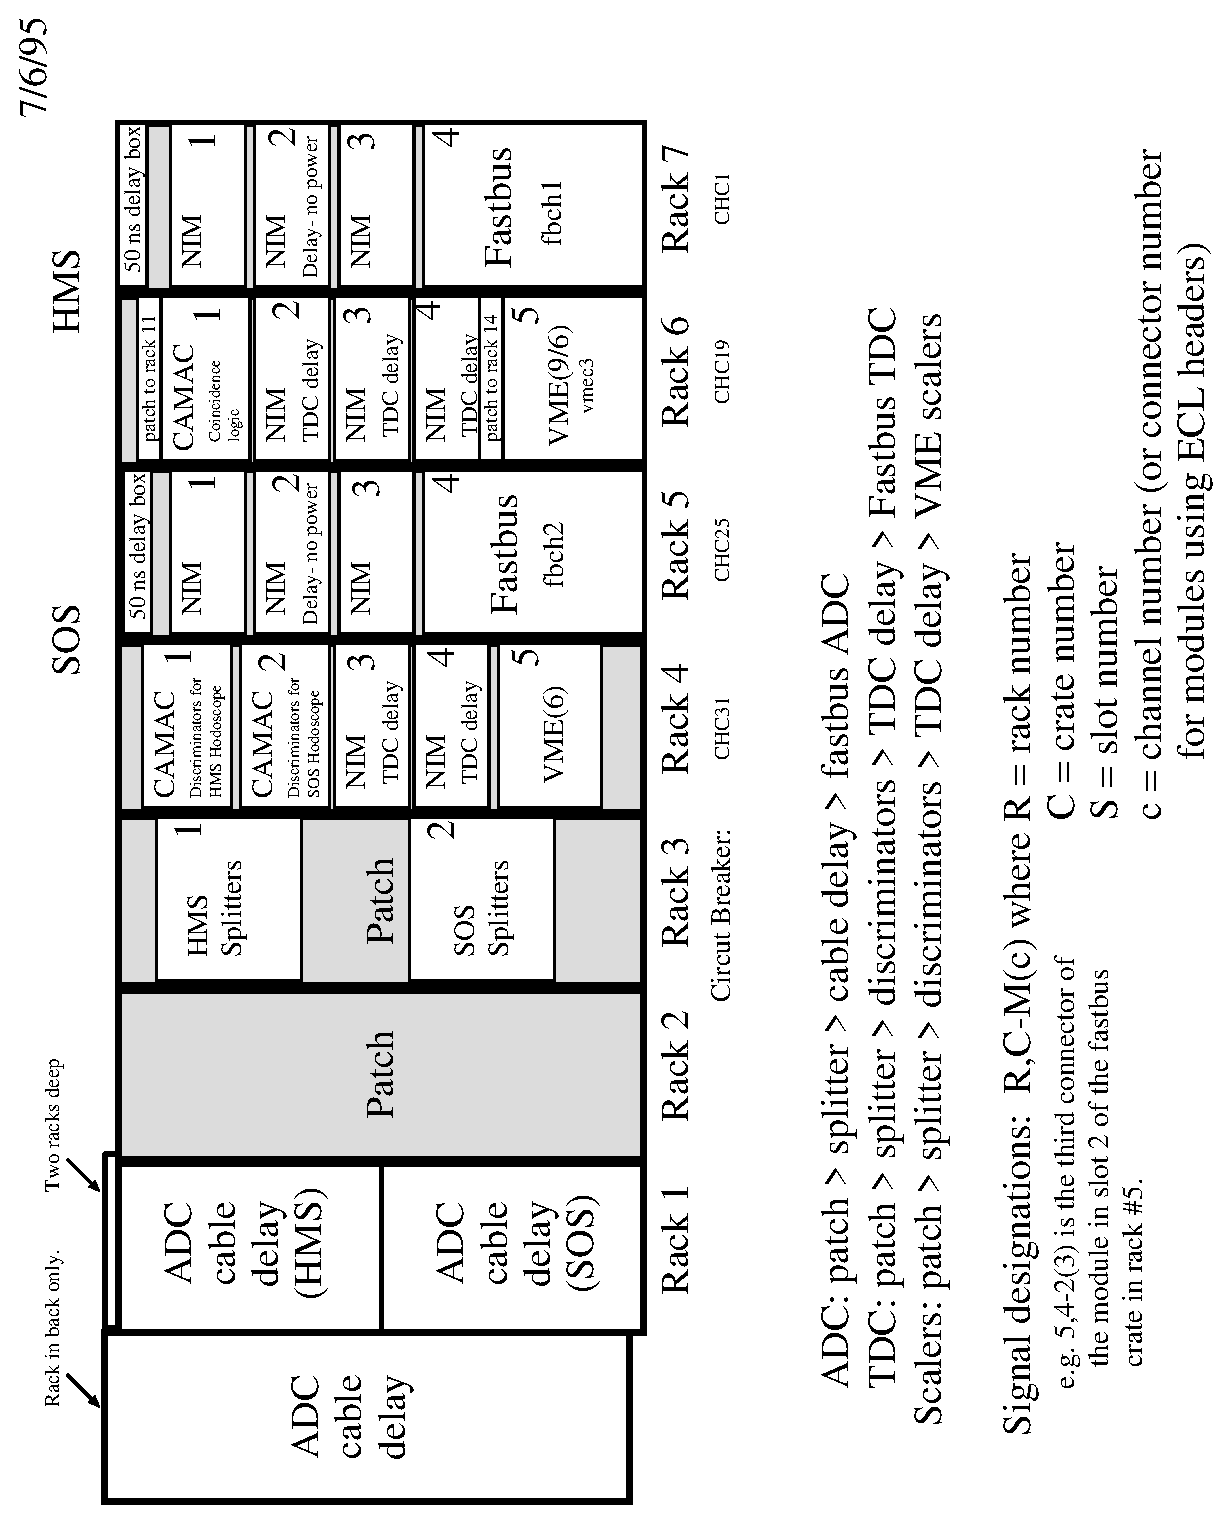
\includegraphics[width=6in]{daq_trig/racks.eps}
\caption{The Primary Racks in the Counting House\label{fig:7.1}}
\end{figure}
Two of these
contain the patch panels where the signals from the hall are
brought to the counting
house. The others contain the fast electronics used to form the trigger and to
readout the data. There are additional racks in the counting house
which contain electronics
related to the beam current monitors and beam rastering system. Figures~\ref{fig:7.2}-
\ref{fig:ts_logic} show the trigger electronics, arranged by detector system. Figure~\ref{fig:hms_trig_logic} depicts
the layout of the HMS trigger electronics.

\begin{figure}
%\htmlimage{thumbnail=0.5,flip=r270}
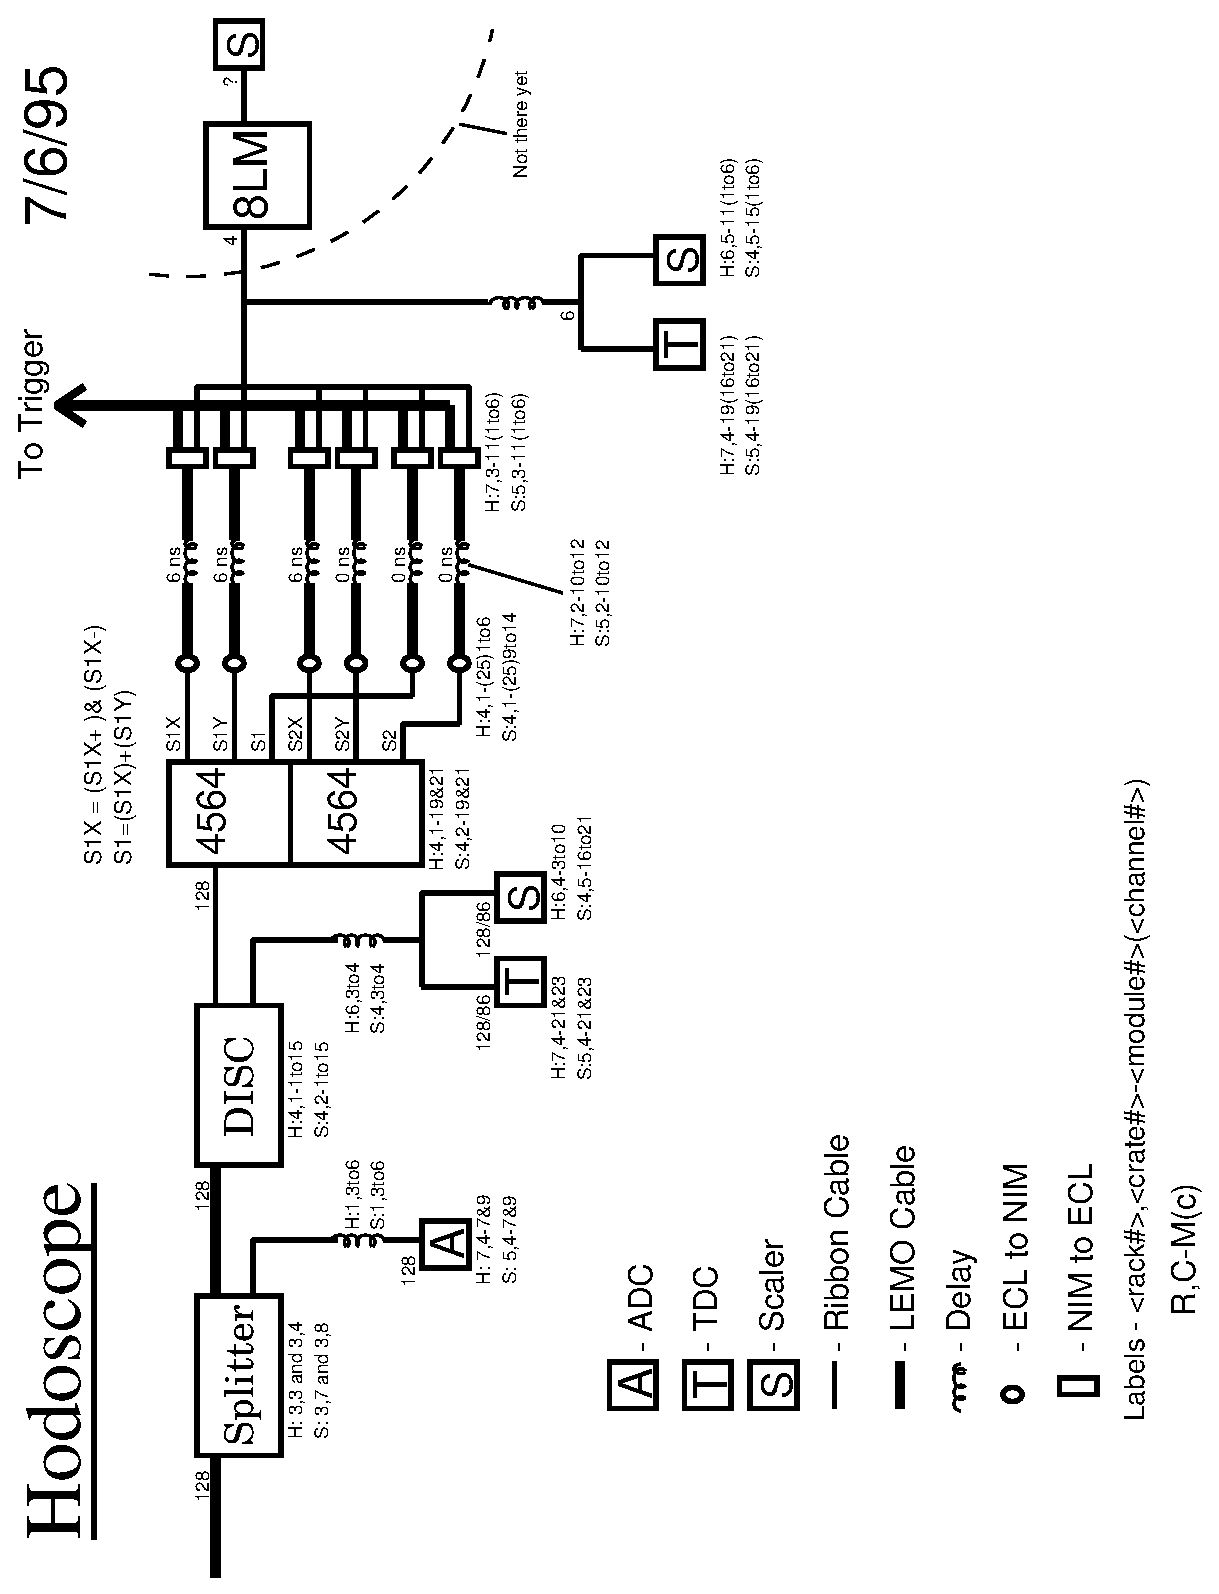
\includegraphics[width=5.8in]{daq_trig/hodoscope.eps}
\caption{Hall~C Fast Electronics (1 of 5) \label{fig:7.2}}
\end{figure}
\clearpage

\begin{figure}
%\htmlimage{thumbnail=0.5,flip=r270}
\includegraphics[width=5.8in,height=7in]{daq_trig/cerenkov.eps}
\caption{Hall~C Fast Electronics (2 of 5) \label{fig:7.3}}
\end{figure}
\clearpage

\begin{figure}
%\htmlimage{thumbnail=0.5,flip=r270}
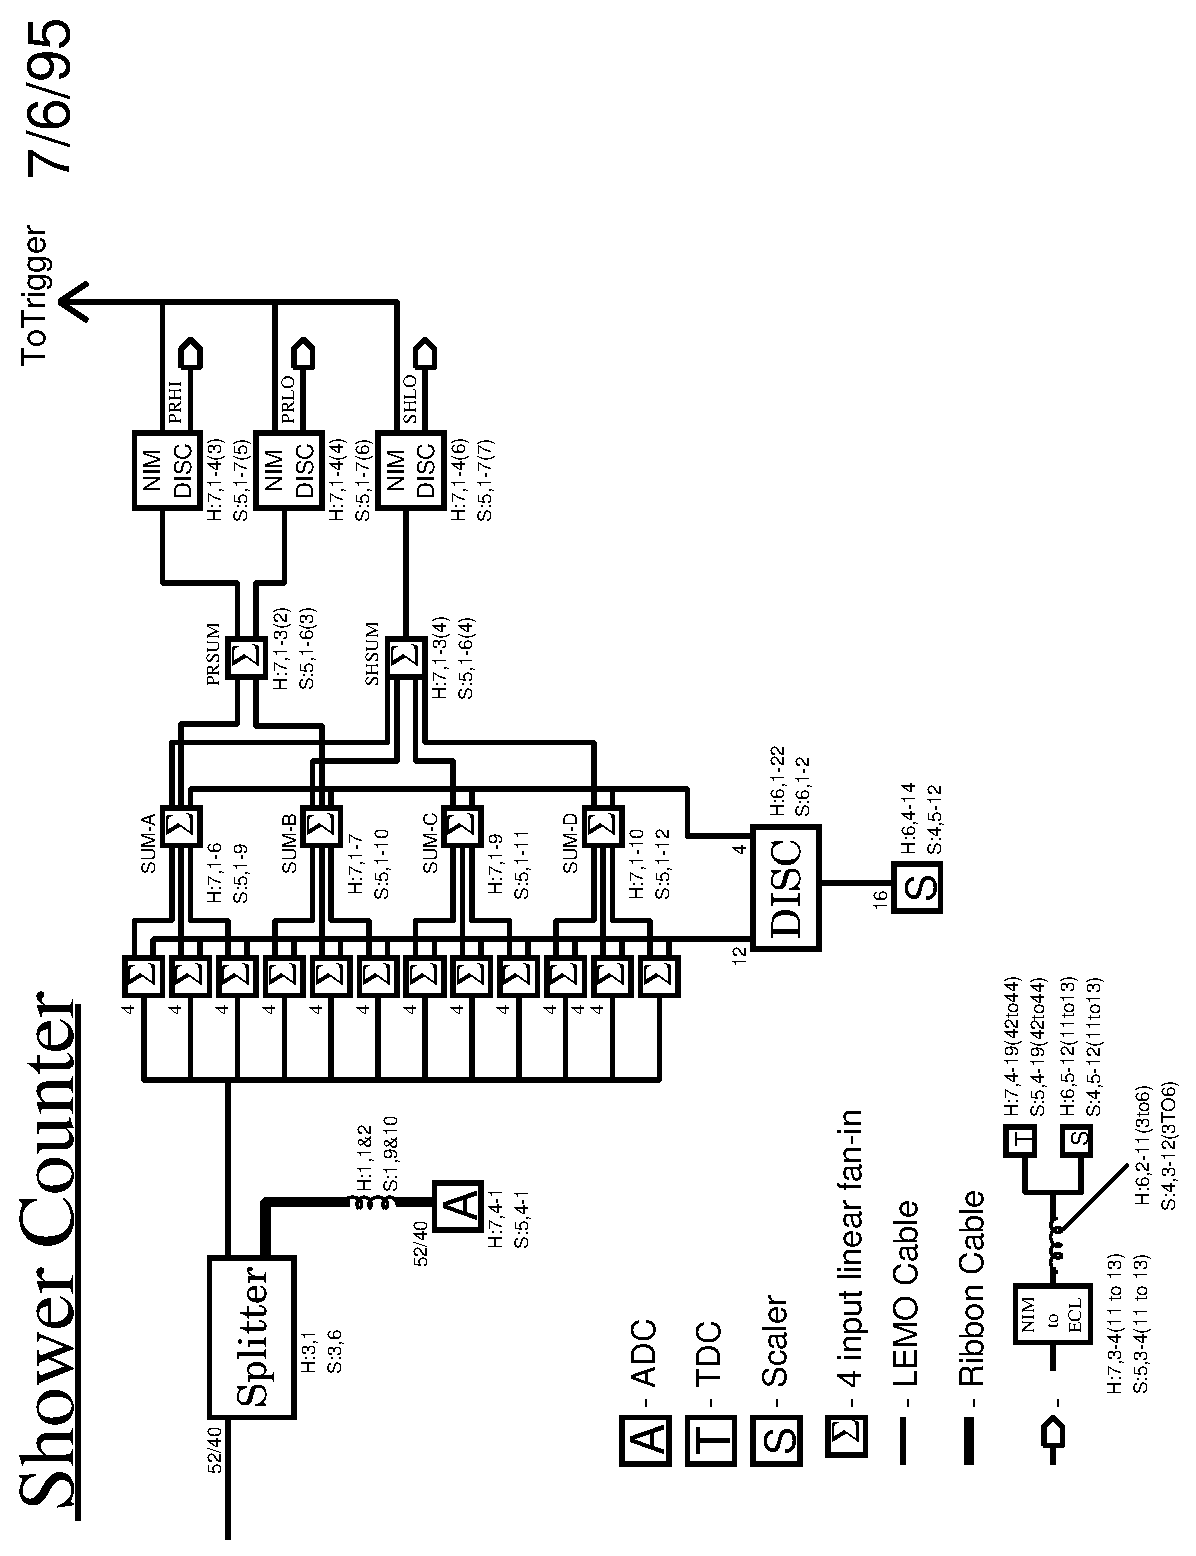
\includegraphics[width=5.8in]{daq_trig/shower.eps}
\caption{Hall~C Fast Electronics (3 of 5) \label{fig:shwr_logic}}
\end{figure}
\clearpage

\begin{figure}
%\htmlimage{thumbnail=0.5,flip=r270}
\includegraphics[width=5.8in,height=7in]{daq_trig/trig_9901.eps}
\caption{Hall~C Fast Electronics (4 of 5) \label{fig:trigger}}
\end{figure}
\clearpage

\begin{figure}
%\htmlimage{thumbnail=0.5,flip=r270}
\includegraphics[width=5.8in,height=7in]{daq_trig/ts_jan99.eps}
\caption{Hall~C Fast Electronics (5 of 5) \label{fig:ts_logic}}
\end{figure}
\clearpage

\begin{figure}
%\htmlimage{thumbnail=0.5}
\includegraphics[width=5.8in]{daq_trig/hms_crates.eps}
\caption{HMS Trigger Electronics\label{fig:hms_trig_logic}}
\end{figure}
\clearpage

\subsubsection{Cabling}

The path that a signal follows from a PMT to the counting house is as
follows.
\begin{enumerate}
\item 30 ft length cables will run from the PMT's to a patch in the focal
plane hut.
\item 250(200) ft length cables run from the HMS(SOS) hut patch along the
spectrometer and through the pipes
under the floor to a patch near the personnel access to the hall.
\item 200 ft length cables run from the patch at the hall entrance
along the hallway wall and up the shaft.  They continue under the
computer floor and up to patches in the counting room.
\item 8 ft length LEMO cables run from the patch to the splitter (see
Figure~\ref{fig:7.1}).
\end{enumerate}
{(\bf Note: Cable lengths are unverified rough estimates.)}
The total length of the cable from the PMT's to the splitter is 560 ns.

Patch cable signal assignments are recorded in the document
\verb|~cdaq/documents/trigger/C_patches.txt|.

The cable runs for the SOS are similar except that an extra 100 ns worth
of cable has been added to the cable run before the splitter.  This extra length
of cable is located in the back of the SOS hut, just before the patch leading
from the hut to the floor of the hall. This  extra amount of cable is (with
great difficulty)
removable and the length has been chosen such that if a coincidence reaction
emits a $\beta = 1$ particle into each spectrometer, the signals will arrive
at the patch simultaneously.  The extra cable is removable to allow for
experiments with a very slow hadron in the SOS to be timed into a
coincidence with an electron in the HMS.

The splitters will make a possibly asymmetric split of the signal, one for the
discriminators, the other delayed for input into ADC's. UVA's design for a
compact splitter box handles 64 channels in 3 inches of 19 inch rack space,
with LEMO inputs which are split into LEMO outputs and into 34 pin headers.
The discriminators have two outputs per channel. One output will be used in
the trigger logic, the other channel will be delayed for input into high
resolution TDC's.

The types of delays for ADC and TDC inputs are :
\begin{itemize}
\item Delay with RG-8 or RG-58 feeding into a box that transfers the
signals to ribbon cable.
\item Digital delay boxes.
\end{itemize}
respectively. These delays are approximately 360 ns. The ADC is
the LeCroy 1881M Fastbus ADC using 34 pin headers for inputs.
The ADC's are configured to have an input termination of 50 ohm with a
fixed ground.

The input termination may be either 50 ohm with fixed ground,
50 ohm with floating ground, or  100 ohm pseudo-differential inputs.
They may also be used as single ended by grounding one pin.

% Not relevant
%The delay for the discriminator outputs must have time delay stability. If
%ribbon cable is used for the delay, we must keep the temperature of the
%cable stable. Dave Mack has found a temperature instability of XX ps per
%degree. We may want to boost the ECL signals just after the discriminator
%so that the signal inputs will still be large at the TDC inputs.

\subsubsection{Coincidence Electronics}

The trigger electronics has switchable 63.5 ns delays on the hodoscope
OR's for both spectrometers. This allows one spectrometer to be delayed
by up to 63.5 ns with respect to the other. For the purposes of computing
the range of velocities that can be brought into coincidence, these delays
shall be considered to have a range of at most $\pm$ 50 ns. This is to
allow room for making either spectrometer come slightly later than the
other and room to adjust the relative timing of the hodoscope planes.

Each spectrometer has essentially identical focal plane trigger logic.
Each hodoscope signal is discriminated with a Phillips 16 Channel
Discriminator Latch (CAMAC Model 7106). Because there is some cross talk
within each group of 4 channels of this discriminator, the inputs are shuffled
so that for single track events, only at most one input of each four
channel group will have a hit. For each of the 4 hodoscope planes, the
tubes on the two sides of the plane are separately ORed together with
the LeCroy 64 channel OR logic unit (4564). The ORed side pairs are
ANDed together resulting in four signals (S1X,S1Y,S2X,S2Y), one for each
hodoscope plane. S1X and S1Y are also ORed to give S1 and similarly the
S2X and S2Y gives S2. These form the 6 Hodoscope signals used in the
Trigger. The above logic is drawn in Figure~\ref{fig:7.2}.

These six hodoscope signals are ECL. They are converted to NIM with
Phillips 16 Channel ECL-NIM converters. The NIM signals are then delayed
with manual switched delays (Phillips 792) with a range of 0 to 63.5 ns.
These delay boxes are used to adjust the relative timing of the
four hodoscope planes.

The NIM outputs of the 4 delay boxes are passed through ECL-NIM
converters. This is to provide a fan out of ECL signals to scalers and
inputs to a parallel logic unit to make coincidences of various
combinations of hodoscope planes for scaling purposes.

Similarly the shower counter signals from the splitter are summed over
individual planes as shown in Figure~\ref{fig:shwr_logic}.
There are 4 planes, each having 12 PMTs. They are
summed in groups of 4 tubes (like the hodoscope, the signals are shuffled to
avoid cross talk). Next the first two planes are summed together to give
PRSUM (preradiator sum) and also all four planes are summed to give SHSUM. The
PRSUM is then passed on to two NIM discriminators, one with a low threshold
and the other with a high threshold. These form the PRHI and the PRLO,
respectively. The SHSUM is similarly passed through a discriminator set low to
give SHLO. These three signals form the shower counter part of the trigger.
The electron trigger logic is shown in Figure~\ref{fig:trigger}.

The NIM outputs for the four hodoscope planes from the ECL-NIM units are
used as inputs to LeCroy 365AL logic units. These units allow for the
blocking of inputs without removing cables and for the setting of coincidence
conditions such as 3/4. The output width on this unit may be adjusted for
appropriate overlap with the other spectrometer. This module also has a
single veto which can be used for coincidences or anti coincidences with a
Cerenkov signal. The other inputs to this logic unit are three signals
from the shower counter (PRLO, PRHI, and SHLO).

In this Logic unit S1 is ANDed with S2 to give the scintillator time of flight
signal STOF, while the remaining four scintillator signals S1X, S2X, S1Y and S2Y
are ANDed together with a coincidence level of 3/4 generating the SCIN
signal. Next the STOF and SCIN signals are ANDed with PRLO (one of the shower
counter signals) with a coincidence level of 2/3, this is vetoed by the
anti Cerenkov signal to give ELLO (electron low). Similarly, the SCIN ANDed with
PRHI and SHLO from the shower counter give  ELHI (electron high). These two
(ELLO and ELHI) are then ORed to generate the ELREAL (electron real). The SCIN
is also vetoed by the Cerenkov to give the PION trigger. See Figure~\ref{fig:hms_trig_logic}.

The PION trigger is
prescaled as desired using a prescaling circuit which is essentially two gate
generators in a loop. The ratio of the widths of these two gate generators
determines the scaling factor. The prescaled pion trigger forms PIPRE. Now, the
ELREAL and the PIPRE are ORed to generate the pretrigger PRETRIG.

The ELREAL is also fanned out to a bunch of diagnostic scalars to
determine double pulsing rates. Both spectrometers will have all
of the above components. But depending on experiment and the particles
being observed some of the components need not be used.

The output of the 365AL for each spectrometer is converted to ECL for
input into a LeCroy 8LM programmable logic matrix. The busy output from
the JLab Trigger Supervisor is the third input into the 8LM.  The
8LM, in parallel, makes the coincidence signal, singles HMS, and
singles SOS.  Each of this signals is generated both with and without
busy for a total of 6 outputs. The three outputs with the busy veto are
the inputs to the Trigger Supervisor. The trigger supervisor can be programmed
to accept any desired prescale fraction of the singles triggers. The unbusy
outputs are counted with scalers to measure dead time and are also used as TDC
inputs.
% Need comment about pedestals

The Trigger Supervisor has gate outputs that must be converted to NIM and
anded with Original Trigger Supervisor inputs to establish the precise
starts for TDC's. These logic will also generate gates of the appropriate
width for the ADC's.

The individual hodoscope PMT discriminator outputs are delayed and fed
into TDC's started by the focal plane trigger for the spectrometer that they
are contained in.  However, a number of higher level signals are sent
(hodoscope OR's, focal plane triggers.) to TDC's started by the other
spectrometer to measure the coincidence timing.

Currently all gate widths in the Trigger logic are set at
30 nsec.  % True?

\subsubsection{Timing Philosophy}

As described above, the SOS signal cables from Hall~C have an extra
amount patched in such that light speed particles in both spectrometers
will arrive at the signal splitters roughly simultaneously. The trigger
electronics for each spectrometer have variable delays with a range of 63.5
ns. Since some of this range is required to adjust the relative timing of
hodoscope planes internal to each spectrometer, we can assume that 50 ns
of dynamic range exists within each spectrometer to adjust the
coincidence timing. If the SOS spectrometer signals are delayed by $t_d$
nanoseconds, then the $\beta$ of particles in the HMS will be
$$\beta_{\rm HMS} = \frac{l_{\rm HMS}}{l_{\rm HMS} + 0.3 t_d}.$$
A similar formula holds for $\beta_{\rm SOS}$.
Assuming spectrometer lengths of 27~m for the HMS and
11~m for the SOS, the 50 ns delays allows for the following minimum momenta
and  kinetic energies in each spectrometer.

\begin{table}
\caption{Nominal HMS/SOS Delay Settings\label{tab:delays}}
\begin{center}
\begin{tabular}{clcrrr}
Spectrometer&$t_d$&$\beta$&pions&protons&deuterons\\
\hline\\
SOS&25&0.595&103.2&693.9&1387.1\\
SOS&35&0.512&83.1&558.7&1115.9\\
SOS&45&0.449&70.1&471.4&942.4\\
SOS&50&0.423&65.2&438.1&875.8\\
HMS&25&0.782&175.5&1179.6&2358.0\\
HMS&35&0.720&144.8&973.5&1946.0\\
HMS&45&0.667&124.8&839.2&1677.6\\
HMS&50&0.643&117.1&787.4&1574.1\\
\end{tabular}
\end{center}
\end{table}

\subsubsection{Cable Delay Calculation}

\begin{table}
\caption{Cable Delay Calculations\label{tab:delay_calc}}
\begin{center}
\begin{tabular}{lccllcc}
Element       &Delay&Cum. Delay&&Element           &Delay&Cum. Delay\\
\hline
Split         & 2   &         2&&NIM-ECL           &  4  & 140\\
              & 8   &        10&&                  &  4  & 144\\
Discriminators&12   &        22&&8LM               & 16  & 160\\
              & 6   &        28&&                  &  4  & 164\\
OR            &10   &        38&&ECL-NIM           &  4  & 168\\
              & 6   &        44&&                  &  8  & 176\\
ECL-NIM       & 4   &        48&&Trigger Supervisor& 48  & 228\\
              &14   &        62&&                  &  2  & 230\\
Delay box     & 6   &        68&&TS lvl translator &  2  & 232\\
              & 2   &        70&&                  &  8  & 240\\
NIM-ECL       & 4   &        74&&Retime wait       &20+  &260+\\
              & 2   &        76&&Retime AND        & 10  &270+\\
SCIN          &10   &        86&&                  &  2  &272+\\
              & 2   &        90&&Delay box         &  2  &274+\\
ELLO          &10   &       100&&                  &  2  &276+\\
              & 2   &       102&&Fan-out           &  4  &280+\\
ELREAL        &10   &       112&&                  &  2  &282+\\
              & 2   &       114&&NIM-ECL           &  4  &286+\\
PRETRG        &10   &       124&&                  &  4  &290+\\
              & 4   &       128&&TDC dead time     & 30  &320+\\
Delay box     & 2   &       130&&                  &     &    \\
              & 6   &       136&&                  &     &    \\
\end{tabular}
\end{center}
\end{table}

Add to this the time that the trigger needs to be delayed for the
coincidence. The TDC input comes from the discriminator, so
the TDC signal time is 21 ns (time to discriminator) +
23 (cable to delay) + 350 (digital delay) + 6 (cable to TDC)
= 400 ns. This leaves about 80 ns for delaying the HMS for coincidences,
retiming with respect to the singles trigger, and ``slop" in the timing.

\subsubsection{Electronics Operating Procedures}

Operating procedures for electronics checkout, changes, etc. follow.
All hardware locations are given in the following format
(module and channel are optional):
\begin{description}
\item{\bf [Spectrometer:
$<$Rack,$<$Crate - $<$Module($<$channel)]}
\end{description}

For example, HMS: 7,4-19(16) means channel 16 for slot 19,
crate 4 in rack 7 (HMS spectrometer FB crate),
and 4,1-1to15 means slots 1 to 15 for crate 1 in rack 4

\paragraph{Hodoscope, Beginning of Run Hardware Checkout}

\begin{description}
\item{[~HMS: 4,1~~~~SOS: 4,2~]}
\end{description}

Set discriminator thresholds (currently set manually, -60 mV default).

\begin{description}
\item{[~HMS: 7,2-10to12~~~~SOS: 7,2-10to12~]}
\end{description}

Set delays for scintillator planes (S1, S2, S1X, S1Y, S2X, S2Y). Delays
should be chosen so that S2, S2X, and S2Y always arrive slightly later
then S1, S1X, and S1Y. This way, the back plane of scintillators will always
determine the trigger time, even if there is a large variation of particle
velocities in the spectrometer. S1 can be set to determine the timing, but
this requires a large delay on the front planes, and takes away from the
amount of delay available for timing in coincidences.

\paragraph{Calorimeter, Beginning of Run Hardware Checkout}

\begin{description}
\item{[~HMS: 7,1-3(2+4)~~~~SOS: 5,1-6(3+4)~]}
\end{description}

Remove any offset in PRSUM and SHSUM. This can be done by setting
the zero for each fan-in channel, or just rezeroing the final fan-ins that
generate PRSUM and SHSUM.

\begin{description}
\item{[~HMS: 7,1-4(3to6)~~~~SOS:5,1-7(5to7)~]}
\end{description}

Set thresholds for PRHI, PRLO (preradiator energy, high and low
thresholds), and SHLO(total energy cut). It will be necessary to take
runs at several discriminator settings and look at the histograms to determine
the correct threshold. SHLO should be set so that the SHSUM spectrum is
cut off just above the pion peak ($\approx$ 250 MeV at P = 800 MeV).
PRLO should be set so that PRSUM is cut off just above the pion peak
($\approx$ 60 MeV), and PRHI should be set so that it contains 90-95\%
of the PRSUM electron spectrum (minimum of $\approx$ 100 MeV).
The histograms hprsum\_prlo,hprsum\_prhi, and hshsum\_shlo show PRSUM
and SHSUM with cuts based on the trigger signals PRLO,PRHI, and SHLO (you can
use hthreshold.kumac to view all of them)

\paragraph{Cerenkov, Beginning of Run Hardware Checkout}

\begin{description}
\item{[~HMS: 7,1-3(1)~~~~SOS: 5,1-6(2)~]}
\end{description}

Remove zero offset from cerenkov fan-in (see Calorimeter).

\begin{description}
\item{[~HMS: 7,1-4(1)~~~~SOS:5,1-7(4)~]}
\end{description}

Set threshold for CER (see Calorimeter). Look at hcer\_sum\_cut (or
execute hthreshold.kumac). The threshold should be set to just cut off the
pedestal event. The threshold should be set high enough that the one
photoelectron peak does not trigger CER.

\paragraph{Trigger, Beginning of Run Hardware Checkout}

\begin{description}
\item{[~HMS: 7,3-5(3+4)~~~~SOS: 5,3-5(3+4)~]}
\end{description}

Set delays coming into ELLO and ELHI. The scintillator signals (STOF
and SCIN) should come after the calorimeter signals (PRHI,SHHI,SHLO)	

\begin{description}
\item{[~HMS: 7,3-5(4)~~~~SOS: 5,3-5(4)~]}
\end{description}

Set the timing for the NOT\_CER veto of the ELLO signal. The phillips
logic module blocks the event if the veto signal is high AT THE TIME OF THE
COINCIDENCE OF THE INPUTS. Therefore, the NOT\_VETO signal must already be 
high
when the other inputs arrive in order to accept the event.

\begin{description}
\item{[~HMS: 7,3-8(2)~~~~SOS: 5,3-8(2)~]}
\end{description}

Match times for ELLO and ELHI coming into ELREAL.

\begin{description}
\item{[~HMS: 7,2-3~~~~SOS: 5,2-3~]}
\end{description}

Adjust HMS(SOS) pretrigger width and timing for coincidence trigger
in 8LM [6,1-13(15and16)]. The coincidence timing window is determined by
the width of the pretriggers coming in, but the TS only looks for the
coincidence trigger 10 ns after receiving the first singles trigger,
so this limits the coin. window, unless you delay the HMS TRIG and SOS TRIG
going into the TS.

\begin{description}
\item{[~HMS: 7,2-3~~~~SOS: 5,2-3~] - Delay for retiming ADC/TDC gates.}
\end{description}

The triggers from the TS muse be retimed with respect to the original
HMS(SOS) trigger in order to insure that the ADC gates and TDC starts come at
the right time. The delayed HMS(SOS) trigger muse ALWAYS arrive after the TS
gates.

\begin{description}
\item{[~HMS: 7,1-1(1to3)~~~~SOS: 5,1-1(1to3)~]}
\end{description}

The ADC/TDC gates are generated here. The width must be set to be
appropriate for the ADC that it is triggering. The delays can be set
independently for the ADC and TDC gates. The TDC starts should 30-50ns
before the earliest signal in the TDC, since the TDC takes a little time
to 'arm' itself after the start. The ADC gate should contain at least 90-95%
of the signal, and should have $\approx$20 ns between the leading edge
of the ADC gate and the start of the ADC signal.

\begin{description}
\item{[~HMS: 7,3-7(1to2)~~~~SOS: 5,3-7(1to2)~]}
\end{description}

The pion triggers are prescaled here. Each gate's trailing edge is
the start for the other gate, so the two gates toggle back and forth. The
pion triggers are passed only when the bottom gate is enabled. If this were
all there was to the circuit, there would be a fixed fraction of the time
in which pions were accepted: f = T$_{bot}$ / (T$_{top}$+T$_{bot}$). However,
the pipregate also acts as a stop for the bottom gate, so only one pion is allowed
thru each time the bottom gate opens. Therefore, the fraction of the time
pions are accepted decreases when the pion rate increases. This allows
running for both very high and very low pion rates without having to
adjust prescaling factors. At low pion rates, (R$_\pi$ $\ll$ 1/T$_{bot}$),
the bottom gate usually times out, and the rate of pions taken is
$$
	R_\pi \times (T_{bot} / (T_{top} + T_{bot}))
$$
which is R$_\pi$ if T$_{bot}$ $\gg$ T$_{top}$. At very high pion rates, the
bottom gate closes very quickly, and the rate is limited by the time before
the gate opens again = T$_{top}$. Therefore, setting T$_{top}$
= 1/(maximum desired pion rate) and setting T$_{bot}$ $\gg$ T$_{top}$
gives a good pion sample for both high and low pion rates.

\subsection {Changes to Kinematics, Beginning of Run Hardware Checkout}

When kinematics are changed, you may have to redo some of the above
settings. If the velocity in the hadron arm changes, you will have to
set the delays to the coincidence trigger again, in order to insure that the
HMS and SOS triggers arrive within the coincidence window (step D4). For
fairly large changes in particle velocity (singles or coincidence experiments)
it may be necessary to adjust the delays in the trigger (steps D1 and D2) since
the cerenkov and shower counter signals may come up several ns later (with
respect to the scintillators) for a slower particle. It may also be necessary
to adjust the ADC gates (step D6)(the TDC's should have enough slop to allow
for the time difference).


\subsection {Regular Hardware Checks (1 per shift or 1 per day)}

\begin{itemize}
\item[{[~~~~]}]{Check visual scalars by eye and in the end of run report files.}
\item[{[~~~~]}]{Check raw ADC/TDC histograms and drift chamber wire maps.}
\item[{[~~~~]}]{Make sure that the hardware and software count of triggers as well
as the scalar counting ADC gates agree.}
\item[{[~~~~]}]{Check the high voltage epics controls.}
\end{itemize}

\subsection {Data (Software) Checks (1 per day, shift, or run)}

See the files check.txt and calibrate.txt in the online documentation
located in the
\begin{verbatim} ~cdaq/documents/analysis_code \end{verbatim}
irectory.

\subsection{Hall~C Terminal Servers}
%
In Hall~C
are located a number of computers and other devices that have
RS232 serial communication/console ports.  It is often essential to connect
a terminal in the counting house to one of these ports
in the course of normal operations or
in order to diagnose
a problem.  Rather than run individual
serial lines for each device at lengths that exceed the recommended lengths
for RS232, several terminal servers are located in Hall~C that multiplex
the communications ports of the computers and devices onto ethernet.  Any
X-terminal in the counting house may then be used to communicate with
any device connected to a terminal server. 

Refer to Table~\ref{tab:hctsvx} to determine the terminal server name and port
number for the device to which you wish to connect. 
To connect to a port, add 2000 to the port number and then type
``telnet hostname portsum''.  For example, to connect vmec3, type
\begin{verbatim}
        telnet hctsv4 2006
\end{verbatim}
After you are finished, be sure to close your connection as the servers
can support only one connection at a time. If you keep the line busy,
nobody else can connect. To close your session type {\tt \verb|ctrl-]|},
then, at the telnet prompt, type {\tt quit}.

If you get an error "telnet: Unable to connect to remote  host: Connection
refused" it probably means that there is already a connection to the port you
are trying to connect to. Look around at the terminals in the counting room: is
there a window open to that port already??  Was somebody else working with that
same port recently who may have forgotten to close the connection?


These tables are for the currently installed terminal servers (December, 2000).
Changes and additions should be expected as the system matures or experiments
change. Change notes should be added using the automatic notation system in the
online version of this
manual. Up to date system status might also be found in\\ 
{\tt ~cdaq/documents/slow\_controls/tserver.tex}.
%-----------------------
\begin{table}[!ht]\centering
\caption{Terminal Server Port Assignments \label{tab:hctsvx}}
\begin{tabular}{|l|l|l|}  \hline
\multicolumn{3}{|l|} {\em Terminal Server hctsv1: HMS HUT } \\
\multicolumn{3}{|l|} { } \\ \hline
\hline
Port  &   Device  & Function\\ \hline
 1    &           & Terminal Access\\
 2    &   sfihms  & ROC2: HMS Drift Chambers\\
\hline
\multicolumn{3}{|l|} {\em Terminal Server hctsv2-ep: G0 Area} \\
\hline
 1    &           & Terminal Access\\
 2    &           & GeN HV mainframes \\
\hline
\multicolumn{3}{|l|} {\em Terminal Server hctsv3: GeN Hut} \\
\hline
 1    &           & Terminal Access\\
 2    &           & \\
\hline
\multicolumn{3}{|l|} {\em Terminal Server hctsv4: Counting House} \\
\hline
 1    &           & Terminal Access\\
 2    &   sfich3  & ROC7: Third Arm Fastbus\\
 3    &   vmec9   & ROC9: Third arm scalers\\
 4    &   vmec5   & ROC5: SOS scalers\\
 5    &   sfich2  & ROC3: SOS PMT Fastbus\\
 6    &   vmec3   & TS0: Trigger Supervisor, HMS scalers\\
 7    &   sfich1  & ROC1: HMS PMT Fastbus\\
15    &   vmec8   & ROC8:M\o ller and Helicity Dependent Scalers\\
\hline
\end{tabular}
\begin{tabular}{|l|l|l|}  \hline
\multicolumn{3}{|l|} {\em Terminal Server hctsv5: Controls racks behind green wall} \\
\hline
 1    &           & Terminal Access\\
 2    &           & vmec10: M\o ller controls\\
 3    &           & vmec11: M\o ller controls\\
 4    &           & vmec19: SOS magnet controls\\
\hline
\multicolumn{3}{|l|} {\em Terminal Server hctsv6: SOS Hut} \\
\hline
 1    &           & Terminal Access\\
 2    &           & ROC4: SOS Drift Chambers\\
\hline
\multicolumn{3}{|l|} {\em Terminal Server hctsv7: Target racks} \\
\hline
 1    &           & Terminal Access\\
 2    &           & vmec4: Target EPICS IOC\\
 3    &           & HMS/SOS Slit controls\\
\hline
\end{tabular}
\end{table}



\subsection{Data Acquisition}

Acquiring coincidence data in Hall C involves the use of 7 computers
running CODA on unix type operating systems.  In addition, the control of
the High Voltage for the Wire Chambers and Phototubes, involves another 3
computers running the EPICS control system.  With the exception of the
Sun system (cdaqs1) used to record data, and the HP-UX system
(cdaqh1)
used to interface to the High Voltage control systems, these computers
normally will automatically boot into the proper state when powered up.


\subsubsection{What Needs To Be Turned On}
In order to acquire data from both the HMS and neutron counters, Fastbus,
VME, NIM, CAEN HV, LeCroy HV and other voltage supplies must be turned on in
several
locations:
\begin{enumerate}
\item HMS detector Hut.
 \begin{itemize}
   \item Acopian power supplies supply $\pm5$ volts to the drift chamber
disriminator cards.  They are located in the short racks under the lead
glass shower counter.  All of these power supplies must be switched
on.
   \item Tall Electronics rack.  Everything in this rack must be power on.
This rack contains.
   \begin{itemize}
    \item Fastbus crate containing Lecroy 1877 multi-hit TDC's for the drift
       chambers.  After powering up, the RESET button should be pressed on the
       VME CPU module to reboot this computer.  The VME CPU is located inside the
       SFI (Struck Fastbus Interface) which is a several slot wide module.
       This module, with it's CPU, functions as the CODA
       Read Out Controller (ROC) 2 and has the internet address \verb|sfihms|.

    \item This CPU may be reset from the Counting House in rack CH03B10
       (just to the right of the two racks containing the Sun/HP workstations
       and disks.)
   \end{itemize}
 \end{itemize}
%%%%%%%%%%%%%%%%
\item SOS detector Hut.  (Accessible only when concrete doors are open.)X
\item SOS electronics shack.
\begin{itemize}
\item Fastbus crate containing Lecroy 1877 multi-hit TDC's for the drift
chambers.
After powering up, the RESET button should be pressed on the
VME CPU module to reboot this computer.  The VME CPU is located inside the
SFI (Struck Fastbus Interface) which is a several slot wide module.
This module, with it's CPU, functions as the CODA
Read Out Controller (ROC) 4 and has the internet address \verb|sfisos|.


\end{itemize}


\item Hall C Counting House.
\begin{itemize}
\item Electronics Racks along wall with outside door.  The electronics in
these racks provide the trigger.  Everything in these racks should be
turned on.  [Reference a layout of this rack]
\begin{itemize}
\item Fastbus crate for HMS - \verb|sfich1| (ROC 1) - rack CH03B07
\item Fastbus crate for SOS - \verb|sfich2| (ROC 3)
%\item Fastbus crate for GeN counters - \verb|sfich2| (ROC 3) - rack CH03B05
\item Trigger supervisor/scalers VME crate (ROC 20) - rack CH03B06
\item Scalers VME crate (ROC 5)- rack CH03B04
\end{itemize}
%%%%%%%%%%%%%%%%%%%%%%%%%%%%%%%%%%%%%%%%%%%%%%%%%%%%%%%%%%%%%%%%%%%%%
\item Electronics racks to the right of the main trigger racks.  The
following items must be powered.
\begin{itemize}
\item Dual Backplane VME crate located at top of rack. (CH03B13)
This crate contains \verb|vmec6|, an
MV167, which is the EPICS controller for the HMS CAEN High Voltage System
and an MV162 which is the EPICS controller for the SOS high voltage.  They
communicate with the HV crates using CAENnet.  The reset buttons on these
CPUs should be pressed after the crate is power up.
\item Dual backplane VME crate located at bottom of left rack.  (CH03B13)
The left CPU, \verb|vmec8|, an MV162,
provides scalers that are used to read helicity dependent rates.  \verb|vmec8|
is also used in the M\o ller polarimeter data acquisition system.
The right hand backplane (which may or may not have a CPU) is not used at
the present time.
The reset buttons on the left CPU 
should be pressed after the crate is powered up.
\item Other electronics used for raster magnet control and Raster/BPM
event by event readout.
\item 10(yes, ten) Mod. Sy403 64 Channel High Voltage System crates
(in racks CH03B16-17) which supply high
voltage to the phototubes and drift chambers in the HMS and SOS.
The Main power
must be on and the HV Enable switch in the up position.  The HV ON light
will only light if at least one channel is on.  Instructions for using the
EPICS control system for turning the channels on are given below.
\end{itemize}
%%%%%%%%%%%%%%%%%%%%%%%%%%%%%%%%%%%%%%%%%%%%%%%%%%%%%%%%%%%%%%%%%%%%%%%%%%
\item Electronics racks to the left of the main trigger racks.
\begin{itemize}
\item Leader variable power supplies supply a threshold voltage to the
HMS and SOS  drift chambers.
They are located in the counting house in rack CH03B10.  The recommended
voltages are (5.5, 5.5, 4.0) for (HMS1, HMS2, SOS) chambers.
\item Reset Panel.
\end{itemize}
\item Gen electronics racks.  All crates should be turned on.
\item Laser.  Located in room above the cable shaft.  (Near the refrigerator).
Consult an expert.
\end{itemize}
\end{enumerate}

\subsubsection{Starting Control Systems}\label{par:hv_ops}
The detector High Voltages are set from the X terminal (hallcxt13) just to
the right of the center of the main control console.
This X terminal should normally be
logged on to \verb|cdaqh1| with the \verb|cvxwrks|
account.

After logging on, control screens for the HMS and the SOS must be started.
Click the left mouse button anywhere on the screen background and select
the ``HMS HV'' menu item and repeat for the ``SOS HV'' item.  The control
screens will take several seconds to start up.
(If a screen fails to
appear after 2 minutes, reboot \verb|vmec1| for HMS or \verb|vmec6| for
SOS, wait 5 minutes and try starting the screen again.  See the section on
rebooting below.)

The operation of the HMS and SOS HV screens are menu driven and mostly self
explanatory.
To turn on the high voltage, the ``Group'' menu must be used to pull up
a control screen for each detector subsystem.  A
global ON option exists for each ``group''.  (There is no ON button that
turns on all the high voltage for the whole spectrometer)
Turning on the high voltage
will set the voltage last stored in the Caen High Voltage main frames.  If
these voltages are incorrect, they can be set with the group screens, or the
restore menu item on the main screen may be used to retrieve a previous
set of high voltage settings.  If permanent changes are made to the high
voltages, these new settings should be saved with the ``Backup'' menu
item.  Note:  Backup and restore operations take an extremely long time
(several minutes).

The column labeled ``Vset'' contains the setpoint for the voltage,
and the column labeled ``Vmon'' contains the actual voltage as read
back from the power supply.  The ``Imon'' column contains the current
drawn by the channel.  The ``Status'' column shows whether the channel
voltage is actually set or not.  Occasionally a channel may trip off
for some reason. This is indicated by the word
``Tripped'' in the Status column.  To correct this, select ``Trip Reset''
under the ``Command'' menu.


\subsubsection{Reconfiguring the High Voltage system}
From time to time, dead channels or High Voltage mainframes may necessitate
the rewiring of the HV cables.  In this case, the EPICS system for the
appropriate spectrometer must be rebuilt.  Consult with someone familier
with this task.  There is a document at

\htmladdnormallink{$\sim$cdaq/documents/slow\_controls/hvcntl.text}
{http://www.jlab.org/Hall-C/document/slow_controls/hvcntl.text}
that gives some more
information about the CAEN HV Voltage system, but it should be used with
caution.

\subsubsection{Setting Data Acquisition (CODA 2.1)}

For a short description of setting up and running data acquisition, also see the
document at \verb|/home/cdaq/documents/data_acquisition/quickdaq_coda2.tex|.

Data acquistion is run from \verb|cdaqs1|.  This machine
has fast ethernet
network interfaces for high speed data acquisition from the Fastbus and VME
front ends and a farm of high speed/capacity disk drives for data storage.

\verb|cdaqs1| is the 20 inch screen just to the left of the center
of the main control console.  This machine should be
logged on with the username \verb|cdaq| and a password that is known to
the shift leaders.\\

%After logging on, start up at least two ``xterm'' sessions by clicking the
%mouse on the screen background and pulling down either the ``xterm'' or
%``small xterm'' options several times.

The first thing to do is to start up the \verb|CODA MASTER| GUI
which allows one to 
control and check coda processes and frontends.
%Use the middle mouse button 
%on the background window and click on \fbox{CODA MASTER}.
%If this does not work,
Start up an ``xterm'' (left mouse button on background window!) 
and type in the command:
\begin{verbatim}
codamaster
\end{verbatim}
(Each Hall C experiment or setup will have a short string that will be
used as a subdirectory under which DAQ, replay and other code is placed.
Examples are ``gen'' for the Polarized target GeN experiment, and ``daq99''
for experiments during 1999 that used the base Hall C equipment.
The environment variable \verb|DAQROOT| will be defined to be the name of
this subdirectory.)
To enable buttons on the CODAMASTER GUI, you have to choose \fbox{Enable buttons}
in the \fbox{Config} menu of the \verb|CODA MASTER|.\\  

If starting up for the first time for a running period, the following
things should be checked.
\begin{itemize}
\item Are all ROC's on-line.  The following ROC's need
to be working: 
\verb|sfich1|, \verb|sfich2|, \verb|sfihms|,
\verb|sfisos|,
\verb|vmec3|,
%\verb|vmec5|, \verb|vmec8|.
\verb|vmec5|.
Click the \fbox{Get Status} button in the 
\verb|CODA MASTER| to obtain the status of the ROCs. They should either be 
``booted'', ``configured'' or ``downloaded''. See section \ref{trouble} 
(Trouble Shooting Procedures) if there is a problem.
\item Is a disk drive with free space properly selected to receive data?
Startup the diskwatch program with the menu selected by clicking the
{\bf middle} mouse on the background of the screen.  There are four 18GB data
partitions available for saving data.  Make sure one with some free space is
selected. See section \ref{disk} for details.
\item Is the CPU free of any errant coda tasks? Do
\verb+ps -ef | grep coda_+ and kill any processes with the name
\verb|coda_er|, \verb|coda_eb| and \verb|rcServer|.
The easiest way to get rid of all the coda processes is to push the
\fbox{KILL ALL} button in the \verb|CODA MASTER|
\end{itemize}

To start up CODA, several processes have to be started using the following
steps:
\begin{itemize}
\item Push {\bf\fbox{Message Logger}} in the \verb|CODA MASTER|.  
(If the message logger does not startup, start it from an
xterm with \verb|cmlog|.)
In the window that pops up, click the \fbox{File} menu and 
select \fbox{Connect}. In the menu \fbox{Options} select \fbox{Update}.  
Hit $<$return$>$ to ignore the dialog box that pops up. 

%\item Push {\bf\fbox{rcServer}} in the \verb|CODA MASTER| to start up the 
%Run Control Server.  
%(If the Run Control Server does not startup, start it from an xterm with
%\verb|rcServer -d cdaq -s gen -m cdaqs1|.)

%\item Push {\bf\fbox{Run Control}} in the \verb|CODA MASTER| to start up the
% Run Control GUI. 
%(If the window does not startup, start it from an xterm with 
%\verb|runcontrol|.) Click \fbox{Connect} to connect the GUI to the rcServer. 
%An error message may pop up. It can be ignored.  

\item Push {\bf\fbox{Run Control}} in the \verb|CODA MASTER| to start up the
Run Control GUI. 
(If the window does not startup, start it from an xterm with 
\verb|runcontrol|.) Run Control starts up the rcServer automatically in the 
background. There is still a window with rcServer messages in it, but it 
starts up iconized.
Click \fbox{Connect} to connect the GUI to the rcServer. An error message
may pop up. It can be ignored.  

\item Push {\bf\fbox{Event Builder}} in the \verb|CODA MASTER|.  (If the
event builder does not startup, start it from an xterm window with\\
\verb|coda_eb -i -s $SESSION -n EB1 -t CDEB|.)

\item Push {\bf\fbox{Event Recorder}} in the \verb|CODA MASTER|. 
(If the event recorder does not start up, start from an xterm window with\\
\verb|coda_er -i -s $SESSION -n ER1 -t ER|.)

\item Push {\bf\fbox{ET System}} in the \verb|CODA MASTER| to start the
Event Transfer system. 
\end{itemize}


Once everything is running, click the \fbox{Configure} button and select a
run type.   The run types are experiment dependent. 
Typical run types available are
\begin{itemize}
\item \verb|coin| (for regular DAQ with beam)
\item \verb|cosmics21| (for cosmic ray tests)
\item \verb|moller| (for beam polarization measurement).
\end{itemize}

Once configured, click on the \fbox{Download} button.  If after several
seconds, a button labled \fbox{Prestart} appears, then the system is ready to
take data.  Otherwise, look at the ``Message Logger'' window
and consult an expert if necessary.



\subsubsection{Taking data}
The DAQ states and transitions which can be executed by pressing the appropriate 
buttons in the Run Control GUI
are shown graphically in Fig. \ref{fig:coda_states}.
Edit the file {\tt /home/cdaq/\$DAQROOT/coda2/cdaq.flags} ({\tt moller.flags}
for M\o ller running) to set/change flags. The keywords have to be on one line 
with no spaces inbetween. Don't forget to save the file.
The values are downloaded at \fbox{Prestart}. The following 
keywords can be specified:\\
{\tt sparse}: Turns on sparsification\\
{\tt buf}: Turn on buffered mode\\
{nped=}: Number of pedestals to be taken at beginning of run\\
{\bf Trigger prescale factors:}\\ 
{\tt ps1=}: HMS single\\
{\tt ps2=}: SOS single\\
{\tt ps3=}: Coincidence\\ 
%{\tt ps1=}: e Single\\
%{\tt ps2=}: B single (This trigger is currently not enabled)\\
%{\tt ps3=}: eB Coinc\\ 
%{\tt ps4=}: eB${\bar P}$ Coinc\\
%{\tt ps6=}: Scaler (should be 1)\\ 
%{\tt ps7=}: Laser (ususally 1)\\ 
%{\tt ps8=}: Cosmics (has only an effect during {\tt cosmics21} running, 
%for {\tt main21} this trigger input is disabled)


\begin{figure}
   \begin{center}
       \framebox{
       \includegraphics[height=8cm]{daq_trig/coda_scheme.eps}}
     \caption{State Diagram for the DAQ System, controlled by the  Run Control GUI} 
     \label{fig:coda_states}
   \end{center}
\end{figure}

To start a data taking run, click the {\bf\fbox{Prestart}} button.  After a few
seconds a {\bf\fbox{Go}} button should appear.  Click this button.

After {\bf\fbox{Go}} is pressed, a ``Run Info'' form will
pop up.  This form should be updated to reflect the running conditions of
the run about to be started.  The form is filled with default values, but
may be overwritten with the values from the last run by clicking on the
{\bf\fbox{Last Run}} button.  The current values may also be save as default
values if several runs with similar conditions are expected.  When the
{\bf\fbox{OK}} button is clicked, the values held in the form will be written 
to the data file and the run will be started.

Please write sensible comments in the ``Comments'' field.  The first line of 
the
comments will appear in the title of the electronic log book entry made for the
run, so it should be reasonable descriptive.

To modify the layout of this form, edit the file
\verb|~/$DAQROOT/coda2/runparms.default|, consulting an expert if necessary.

To pause/resume a run, use the {\bf\fbox{Pause}}/{\bf\fbox{Go}} buttons on
the pause GUI. 

A run will end if either you click the \fbox{End} button or the event
limit or the data limit (whichever is first) is reached. Event and
data limit can be specified in the \verb|Run Control| GUI. Enter a
number in the appropropriate field and hit $<$return$>$.  Our CODA
system has been configured to allow runs with sizes greater than
2GByte in size. This is done by automatically closing the data file
and opening a new file. Thus a long run will be split into several
segments. The run filenames have the form e93038\_XXXXX.log.N, where N
is the segment number, starting with 0.



\subsubsection{What To Do When Disk Space Runs Out}

\label{disk}
\verb|cdaqs1| has several (As of December 1998, there are 4)
disk partitions of 18 GB each.  The usage of
disk space can be monitored with the ``diskwatch'' screen which is started
from the pop-up menu (middle mouse button on background window).

This windows shows the amount of disk space free on the current disk.
If the free space is 1\% or less, the \fbox{Change Disk}  button should be
pressed.  ``diskwatch'' will then display an empty disk which should be
confirmed with the ``OK'' button.

The data on these partitions is backed up to the mass storage silo
automatically.  Data is deleted from the Hall C data disks manually.
Steve Wood will normally take care of deleting data from the disks, but users
may delete data that has been backed up to the silo with the following
procedure.

Type

\begin{verbatim}
	partition_check N
\end{verbatim}

where N is the number of next partition that you want to use for data taking.
(For example, if data is currently being written to \verb|/cdaqs1/data4|, the 
next
partition to be used will be \verb|/cdaqs1/data1| and thus the command
\verb|partition_check 1| should be issued.

If there are data files on the disk and it is safe to delete them, a prompt 
will appear asking all the files on the partition should be deleted.  
It is safe to
type yes.  At this point all the data files on that partition will be deleted
so anyone trying to replay those runs will need to request them from the silo.

If \verb|partition_check| does not give the option to delete the files, and no
data has been written to the partition for more than 12 hours, please contact
Steve Wood.

To check that the automatic backup is working, do \verb|ls $STAGE| from %$
time to time to see if it contains recent runs.  The STAGE directory is where
runs get queued up to be written to tape.

% HERE Trouble shooting
\section{Trouble Shooting Procedures}
\label{trouble}
When coda crashes usually one of the ROCs or one of the processes got sick and
has to be restarted. The error messages are not always clear. It is 
recommended to try to execute the desired transition again before you start 
rebooting frontends. Often just the connection to the database got lost, which 
can be easily recovered (see below).
If a transition gets stuck because a component failed, it usually takes some 
time until \verb|Run Control| reports back that e.g. {\em Download failed}.
You can try to stop a transition with the \fbox{Cancel} button in the 
\verb|Run Control| GUI. After transition failure and after reboots you 
should always click the \fbox{Reset} button in the \verb|Run Control| GUI and 
configure the run type again, before you start downloading again.   

\begin{itemize}

\item {\bf The connection to the database got lost.}\\
Occurs usually during ``download'' or ``prestart''.
Typical error message: {\em Failed to connect to msqld on cdaqs1}\\
Click \fbox{Reset} in the Run Control GUI and then exit the 
\verb|Run Control| GUI and restart it again. Press the 
\fbox{Connect} button and procede with \fbox{Configure} and 
\fbox{Download}.

\item {\bf Power Outage in the Hall/ sfihms problem}
If Hall C looses power, sfihms (ROC2) (down in the HMS hut) usually looses 
its memory 
and has to be reprogrammed. Detailled description is found in section 
\ref{sfihms}.  

\item {\bf A ROC died}\\
Reboot the particular CPU:  See section \ref{rebooting} for information on
rebooting ROCs.

\item {\bf EB or ER died}\\
Kill EB {\bf and} ER with {\em Ctrl-C} and restart.
To check if they are alive go to the particular 
window and hit a few times $<$return$>$. The prompts
{\em cdaq::ER1$>$} and {\em cdaq::EB1$>$} should appear. You can also use the 
\fbox{Get Status} in the \verb|CODA MASTER| to check the status.

\item {\bf Download Failure} A possible reason for a fail during download
is the following:
Due to repeated downloads the memory of 
the CPUs gets fragmentated and in particular for the older boards with 
smaller memory it can happen that the allocation of the event buffers 
fails. 
If logged into the CPU one would see a message of the type:\\
{\em daLogMsg: partIncr: Cannot malloc a single memory Block for 
data bufs ...}\\ 
In this case one has to do a hardware reboot of the CPU.
Try to \fbox{Cancel} and \fbox{Reset} the transition and proceed with 
\fbox{Configure} after the CPU is rebooted.

\item{\bf Prestart Failure} If Prestart fails some of the components 
might already have prestarted, i.e. they are in the {\em paused} state.
If after eventual reboot, \fbox{Cancel} and \fbox{Reset}, 
i.e. before you try to 
\fbox{Configure} again, some of the components (including EB 
and ER) should still be in {\em paused} state, you have to 
reset them by clicking \fbox{Exit} in the \verb|CODA MASTER| for the 
particular component. After the status of all componenets is either 
{\em booted}, {\em configured} or {\em downloaded} you can proceed with 
\fbox{Configure}.

\item{\bf End Failure} Similarly to the Prestart Failure a fail during End 
can leave components in a state {\em ending}. Exit the ROCs as
described for Prestart Failure. 
Most End Failures make the Event Builder and/or 
Event Recorder unhappy. It's always a good idea to kill and restart 
these two processes after an End Failure.

\item{\bf DD system} The DD system is the memory where the 
Event Builder writes to and the Event Recorder reads from. After a crash 
it is always a good idea to clean the DD system from possible contamination.
In an ``xterm'' type the command \verb|dd_cleanup|. 

\item {\bf No trigger rate at beginning of run or trigger rate goes to 0 
during run}\\
First thing to do is to check the state of the Trigger Supervisor: Click 
\fbox{CHECK} in the \verb|CODA MASTER| and then \fbox{State} in the 
window that pops up. This displays the current state of the TS. If 
\verb|TS Go| and \verb|TS TRIGGER| are enabled and \verb|TS Busy| is 0
then the DAQ is waiting for triggers. 
The two most popular reasons for the absence of triggers are: 
HMS HV down (check the HMS HV display) and prescale 
factors set too high (Check the flag file: \verb|~/\$DAQROOT/coda2/gen.flags|).
Less likely is a hardware failure of one of the components in the electronics
(e.g. the 8LM). In any case this is not a DAQ problem.\\
A \verb|TS Busy| equal to 1 indicates that the TS is not accepting 
triggers anymore which is a DAQ problem.\\
The easiest 
thing to do in this case is to kill all processes (Use the \fbox{KILL ALL} 
button in the \verb|CODA MASTER|)  and reboot all ROCs 
(hardware reboot recommended, see section \ref{rebooting}). However people 
experienced problems with this radical strategy. The advanced idiot 
might try to recover the system in a more controlled way as described in the
following.\\

If the Trigger Supervisor (TS) does not accept triggers anymore, this can 
have two reasons:\\
1. The buffers of the ROCs are full and are not flushed by the 
Event Builder. This indicates an EB or ER problem. The ROCs are most likely 
still ok.\\
2. One of the ROCs died and the TS doesn't receive the Acknowledge from 
this ROC anymore.\\
To see which of the two cases has occured use again the ``ROC and Trigger 
Supervisor Checkout'' window (if not up, click \fbox{CHECK} in the 
\verb|CODA MASTER|). Check the Buffer Status of all ROCs by clicking the 
approriate button. A listing of the allocated memory appears. In the third 
line (column 2 to 4) the number of total (allocated), free and busy (used) 
buffers in the event pool is displayed. If in one of the ROCs the number
of free buffers should be 0, then it's most likely an EB or ER problem.\\
If this is not the case, it is most likely one of the ROCs which has a 
problem. If you hit the button \fbox{State} to get the TS state the Branch
Status is displayed and at least on one branch the \verb|Strobe| and 
\verb|ACK| should be one, indicating that the sick ROC is on this branch. 
Unfortunately the TS does not provide the information which ROC it is.
Use the \fbox{Get Status} button in the \verb|CODA MASTER| or login
to the ROCs as described in section \ref{login} to find out which ROCs 
have a problem.\\

In any case you can still try to \fbox{End} the run, which most probably
will not work properly. You might have to kill Run Control and start it up
again. Even if you use the \fbox{KILL ALL} button in the \verb|CODA MASTER|
(which is probably the appropriate thing to do in this case) you might still
have the problem that some of the ROCs will stay in the state {\em active}). 
In this case you have to exit them with the \fbox{Reset} buttons in the
\verb|CODA MASTER|. If all the componenets are in the state {\em booted},
{\em configured} or {\em downloaded} you can proceed with \fbox{Configure}
and \fbox{Download}

\item {\bf Something that is alive is not necessarily not sick.}  If it is not
clear if all the coda components are working or not, or if you get confused 
about which components need to be restarted, all the components on the Sun 
can be killed with the \fbox{KILL ALL} button in \verb|CODA MASTER| which 
is equivalent to executing the command:
\begin{verbatim}
		~/$DAQROOT/coda2/scripts/coda_cleanup
\end{verbatim}
\end{itemize}


\subsubsection{Remotely Rebooting Crashed or Corrupt VME CPUs}

\label{rebooting}
A software reboot can be done with the \fbox{Reboot} buttons in the 
\verb|CODA MASTER|. This does not always work. Sometimes it's necessary to do 
a hardware reboot. In very rare cases it is necessary to power cycle the 
crates.   
Hardware reboot of all the readout controllers can be done from the 
counting house. See Table \ref{tab:CODA_resets} for reset button locations. The
CPU's located in the counting house are rebooted by pressing the RESET
button on their front panels.  CPU's located in the hall can be reset 
using the {\tt rebootpanel} application which runs on {\tt cdaqs1}.
\begin{center}
\begin{table}[hbt]
\begin{tabular}{|l|c|l|l|}\hline
CPU    & ROC \# & CPU Location               & Reboot button location \\ \hline
sfich1 & 1      & Counting House CH03B07,4-18 & {\it sfich1}          \\
sfich2 & 3      & Counting House CH03B05,4-15 & {\it sfich2}          \\
sfich3 &        &                             & {\it sfich3}          \\
sfisos & 4      & SOS shack                   & {\it sfisos}          \\
sfihms & 2      & HMS hut                     & {\it sfihms}          \\
vmec3  & 20     & Counting House CH03B06      & {\it vmec3}           \\
vmec5  & 5      & Counting House CH03B04      & {\it vmec5}           \\
vmec8  & 8      & Counting House CH03B13      & {\it vmec8}           \\
vmec9  & 9      & Counting House CH03B21      & {\it vmec9}           \\
\hline
\end{tabular}
\begin{tabular}{|l|}
Items in {\it italics} refer to buttons on the {\tt rebootpanel} GUI.\\
\hline
\end{tabular}
\caption{CODA Read Out Controllers reboot button locations\label{tab:CODA_resets}}
\end{table}
\end{center}
It might take a while for the CPU's to reboot.  (The Fastbus
CPU's are the slowest)
The cmlog window will show a message when a particular ROC has rebooted.

\subsection{ROC Login} \label{login}  
To see if a ROC is alive you can connect to the particular CPU
by using the middle mouse button and selecting the CPU you want,
or by {\tt telnet}'ing through the appropriate terminal server
port. See Table~\ref{tab:hctsvx} for a list of port assignments.
For example, to connect to ROC4, type
\begin{verbatim}
        telnet hctsv4 2007
\end{verbatim}
A window will pop up and you will
be logged in. The prompt \verb|->| indicates that you are on the vxworks 
shell.
Type \verb|i| and hit $<$return$>$ to get a listing of the running tasks.
The last item of this list should have the Name {\em ROC} and the Status
{\em Ready} or {\em Pend}. If it does not exist or its status is 
{\em Suspended}, you have to reboot the CPU.\\
You can change to the ROC shell by typing \verb|exit| and 
hitting $<$return$>$ twice. A ROC specific prompt should appear, e.g. 
\verb|cdaq::ROC1>| for sfich1. If this prompt does not appear the ROC 
is sick and the CPU has to be rebooted most likely. With \verb|ctrl-c| 
you can switch back to the vxworks shell. On the ROC shell a set of commands
is available. As an example you can get the status of ROC1 by typing 
\verb|ROC1 status|. This is identical to clicking the button 
\fbox{Get Status} in the \verb|CODA MASTER| but more reliable.     
Be careful when you are logged into the CPU. Misstyped commands can 
hang up everything.  
To logout use \verb|ctrl-]|. At the telnet prompt type \verb|q|.
Generally it's a good idea to keep a window for each ROC open all the times. 
In case of problems the displayed messages might be helpful. 

\subsection{Reprogramming sfihms}
\label{sfihms}
If HALL C looses power ROC 2 might have lost its memory. Already a short power
glitch could cause this. A symptom is that the CPU doesn't reboot anymore.
Reloading the memory can be done from upstairs with the following 
procedure:\\

\noindent
Use an ``xterm'' to login to the terminal server with \verb|telnet LATSRV|.
Username is \verb|cdaq| and Password is \verb|cntrlme|.
Access then the CPU with \verb|set host/lat hcc2|. Password is \verb|vx4daq|.
Hit \verb|<return>| and at the {\em [VXWorks Boot:]} prompt type \verb|c|
to change boot parameters. 
The following list displayes the correct boot parameters for ROC2:\\

\begin{verbatim}
boot device          : dc 
processor number     : 0 
host name            : cdaqs1 
file name            : ~/KERNELS/vx2306_DECFD 
inet on ethernet (e) : 129.57.168.183:fffffc00 
inet on backplane (b): 
host inet (h)        : 129.57.168.15
gateway inet (g)     : 
user (u)             : cdaq 
ftp password (pw) (blank = use rsh): 
flags (f)            : 0x20 
target name (tn)     : sfihms 
startup script (s)   : ~/$DAQROOT/coda2/boot/sfihms.boot 
other (o)            : 
\end{verbatim}

The parameters are listed one by one. Each time you 
hit return the next one is listed until you are back on 
the {\em [VXWorks Boot:]} prompt. For each parameter that is wrong
type in the correct one. Don't try to delete 
wrong parameters just type from there where the cursor is. If you misstype 
don't try to correct just hit return and when you are finished with the list 
start again. When you are done, go through the list again and check all 
entries.
Back at the {\em [VXWorks Boot:]} prompt type \verb|@|
which boots the CPU.\\ 
Use \verb|ctrl-\| to exit and then \verb|lo| to logout from the terminal 
server. 

\subsection{Rebooting other stuff}
There are also a number of CPU's running EPICS and other controls
software.  If controls for High
Voltage or Magnets are not functioning, they may need to be rebooted.
Table \ref{tab:EPICS_resets} gives the location and function of several 
CPU reboot buttons not already listed in Table \ref{tab:CODA_resets}.
Many of these resets are accessed by running the application
{\tt rebootpanel} from an X-session logged in to cdaqs1 (user cdaq).
\begin{center}
\begin{table} [hbt]
%\begin{tabular}{|l|l|l|l|}\hline
\begin{tabular}{|p{1.8in}|p{0.8in}|p{1.5in}|p{1.1in}|}\hline
Function             & CPU    & CPU Location            & Reboot \\ 
                     &        &                         & Button \\\hline
HMS Cryo \& Rotation & vmec2  & HMS Hut                 & {\it vmec2}     \\
SOS HV               & vmec6  & CH03B13,1-11            & {\it vmec6}     \\
M\o ller Cryo,Tgt,Sol  & vmec10 & Near Power Supplies     & {\it vmec10} \dag   \\
M\o ller Quads         & vmec11 & Near Power Supplies     & {\it vmec11} ***\\
Beam Curr, EPICS Rptr& vmec15 & CH03B12-left            & {\it vmec15}    \\
HMS Hall Probes Read & vmec18 & HMS Shield House        & {\it vmec18}    \\
SOS mag controls     & vmec19 & Near Power Supplies     & {\it vmec19}    \\
HMS HV               & vmec20 & CH03B13,1-1             & {\it vmec20}    \\
Slit Box Controls    &        & Pivot Racks             & {\it slitbox}   \\    
Solid Tgt. Rotator   &        & Behind Green Wall       & {\it STGTROT}   \\    
Solid Tgt. Lifter    &        & Behind Green Wall       & {\it STGTLif}   \\  
M\o ller Coll \& Tgt   &        & Behind Green Wall       & {\it MolCol}    \\   
HMS Dipole PS Comm.  & Eldatic& HMS Shield House        & {\it PDS}       \\
HMS Dipole PS Contr. & Dipole & HMS Shield House        & {\it Eldatic}   \\
HMS Q1 Controls      & HMS Q1 & HMS Shield House        & {\it HMSQ1}     \\
HMS Q2 Controls      & HMS Q2 & HMS Shield House        & {\it HMSQ2}     \\
HMS Q3 Controls      & HMS Q3 & HMS Shield House        & {\it HMSQ3}     \\
Fast Raster IOC      & IOCHLC2& HC01Z07                 & {\it IOCHLC2} * **  \\
\hline
\end{tabular}
\begin{tabular}{p{5.5in}}
Items in {\it italics} refer to buttons on the {\tt rebootpanel} GUI.\\
\dag If you reboot VMEC10 (iochc10) you must then RESTORE the Moller cryo saved
parameters. Use the popup menu given by the small blue box on the bottom center
of the M\o ller cryo overview page. Do a "iochc10:NORMAL RESTORE" and keep
hitting ENTER when the popup dialog screen prompts you.\\

* May also be reset from MCC using a software reset.\\

** This reset generates an FSD! Contact MCC first.\\

*** Do not reboot vmec11 (iochc11) unless requested by MCC.\\
\end{tabular}
\caption{EPICS IOC and Device reboot button locations\label{tab:EPICS_resets}}
\end{table}
\end{center}

A reset switch has been moved up to the counting house for the HMS carriage
rotation. One should use this button if the rotation GUI shows interlocks. If
the interlock is real, then the reset button will not clear the interlock. One
needs to press and hold the button for at least 1 to 2 seconds to clear the
Sumito motor controllers. The reset button is located next to the rotation kill
button, on the left section of the counting room console.

\subsection{Online Data Replay}

The Hall~C online data replay is run by a
software package termed the Hall~C engine.
Figure~\ref{fig:7.8} is a flow chart of the Hall~C engine software in which

%hcftest
\begin{figure}
\includegraphics[height=7.5in,width=6in]{daq_trig/engine_flowchart.eps}
\caption{Hall~C Software Engine}
\label{fig:7.8}
\end{figure}

the important codes are named and organized.
Figure~\ref{fig:7.9} is an enhanced view of the HMS event reconstruction section

%hcftest
\begin{figure}
\includegraphics[height=7.5in,width=6in]{daq_trig/recons_flowchart.eps}
%\vspace{8.0in}
\caption{HMS Event Reconstruction Software Engine\label{fig:7.9} }
\end{figure}

of Figure~\ref{fig:7.8} which also lists the functions performed by the codes.
These flow charts and other useful documents, diagrams, and
figures may be found in
\begin{verbatim} ~cdaq/documents. \end{verbatim}

Of particular interest is a document entitled \begin{verbatim}
how_to_replay.txt \end{verbatim}
which
is a step by step outline for a new user describing how to replay runs.
This document may be found in
\begin{verbatim} ~cdaq/documents/analysis_code. \end{verbatim}


\chapter{Analsys Software}

% See what can be lifted from the Hall A manual


%\section{The Solid Target Ladder}

The scattering chamber has two target ladders associated with it,
a cryogenic target ladder and a solid target ladder. To change
from the cryogenic target ladder to the solid target ladder, one has
to:

\begin{itemize}
\item{Move the cryogenic target ladder to its home position.}
\item{Rotate the cryogenic target ladder over 90 degrees. This removes
the cryotargets from the beam line, and moves them out of the spectrometer
acceptances.}
\item{Insert the solid target ladder and select the appropriate target.}
\end{itemize}

\noindent To install the cryogenic target ladder again, one has to reverse the
process:

\begin{itemize}
\item{Move the solid target ladder to its home position (completely out
of the way).}
\item{Rotate the cryogenic target ladder back into place (-90 degree
rotation).}
\item{Select the appropriate target.}
\end{itemize}

We have four different solid target systems currently in use in the
Hall C Scattering Chamber.  There is a solid target attached directly
to the cryotarget and three versions of the independent solid target
ladder system.

The solid target that is attached to the bottom of the cryotarget is
often referred to as the optic target.  This target is a system of
aluminum and carbon foils arranged at different locations and heights
relative to the beam.  The foils provide cryotarget window
calibration and loop target spectrometer optics calibration.  The
various targets are brought into the beam by simply closing the
vertical height of the cryotarget stand and a ``scan'' can be made
that spans the length of the cryotarget in discrete steps on window
convection data taken.  This system replaced the earlier ``slanted
target'' system.

The independent solid target system has three different ladders which
mount interchangeably to the same mechanism.  This mechanism
provides for a telescopic guidance system with good accuracy
and stability as well as vertical, and rotary control.  The rotary mechanism also
has an integral rotary water feed thru for high power solid target
runnings. 

The three solid target ladders use identically sized interchangeable
variable thickness solid targets.  They use a common target mounting
system.  The three ladders currently available are:

\begin{itemize}
\item{Un-cooled target ladder with a standard solid target position.
This is for 0-30 $\mu$A rastered beams for materials with good
conductivity and high melting points.}
\item{Water cooled target ladder with 6 standard solid target
positions.  This is for 0-100 $\mu$A beams that are rastered.  These
can handle any material.}
\item{Combination water cooled solid and water target.  This target
has, in addition to 5 solid target positions, a new water cell.
The water cell is 1 cm thick and has entrance and exit windows of 0.1
mm (~.005 in) aluminum.  The water cell is all machined and welded to
the bottom of the solid target ladder.}
\end{itemize}

In some cases the solid targets will be cooled with water to prevent
destruction of the targets by a high current beam. If this is the case
make sure that the
cooling water is indeed flowing before the experiment starts.
{\sl Failure to do so may cause loss of the targets}. Often we
do not have to use water cooling. This is the case when we are
rastering the beam, or are dealing with solid target
materials with excellent thermal conductivities (like pyrollytic
graphite or ceramic BeO) and currents less than or equal to 30 $\mu$A.

In all cases, as we may use these targets in conjunction with a high
energy, high current beam a large level of radiation may be induced
in these targets.

The main safety issue concerning the non-special targets is that
they will be radioactive (``hot") after they have been
exposed to the JLab beam for an experiment.
Targets may not be removed from the target chamber ot transported from the Hall without 
concurrence by the RCG. An SRWP specifies the requirements for target removal and/or 
transport. Targets which have been surveyed and released by the RCG will be stored in a 
second fire safety cabinet which has been designated for target storage and is located in 
the hall.

Since the targets may be water cooled, we will induce a slight
radioactive level in the cooling water. However, the cooling water
system is a closed loop, and calculations performed by the Radiation
Safety group indicate that the radioactive level induced is minimal.
Also, to ensure that the cooling water is indeed a contained system
and can not leak out to the environment, the pumping system causing
the water to flow is placed in a tray.

\subsection{Special Targets}

Some of the solid targets require special attention. In some cases
mishandling of the targets is relatively innocent, like in the case
of the natural {\bf Calcium} target. This material, when exposed to air,
will oxidize, resulting in a large oxygen content in the target.
Store natural Calcium always in an argon-filled or vacuum closed
case, or in an oil solution. Calcium can be handled in air for a limited
amount of time (a few hours) if handled with a layer of oil.

Other special targets may pose a safety concern. At this
moment the only twos special target materials we own are ceramic
{\bf Beryllium-Oxide (BeO)} and {\bf Beryllium (Be)}.
In solid form, BeO is completely safe under normal conditions of use.
The product can be safely handled with bare hands.
However, in powder form all Beryllia is {\bf toxic} when airborne.
{\bf Overexposure to airborne Beryllium particulate may cause a
serious lung disease called Chronic Berylliosis. Beryllium has also
been listed as a potential cancer hazard. Furthermore exposure to
Beryllium may aggravate medical conditions related to airway systems
(such as asthma, chronic bronchitis, etc.).}
Since beryllia are mainly dangerous in powdered form, do not machine,
break, or scratch these products. Machining of the Beryllia can only
be performed after consulting the EH\&S staff.
It is good practice to wash your
hands after handling the ceramic BeO. If handling the pure Beryllium
target wear gloves and an air filter mask.

\subsection{Storage}

The targets {\bf must} be stored in a safe, locked place tagged with the
appropriate radiation signs. At this moment we use a small yellow
fire safety cabinet for this purpose. The cabinet is stored in the
little backroom of the Hall~C counting house. The key of the target
storage cabinet can be found in the Hall~C key box, hanging on the
wall next to the Hall~C counting house entrance.
Targets may not be removed from the target chamber or transported from the hall without 
concurrence by the RCG.  An SRWP in the counting house specifies the requirements for 
target removal and/or transport.  Targets which have been surveyed and released by the 
RCG will be stored in a second fire safety cabinet placed downstairs in Hall~C,
that has been designated for target storage.

Since we will typically have
Be and/or BeO targets stored in this cabinet too, also signs indicating
the presence of Beryllium materials (``Beryllium Storage")
are tagged to this cabinet. The Material
Safety Data Sheets for Beryllia are included in the storage cabinet.



\section{Bremsstrahlung Radiator}

The Bremsstrahlung radiator consists of a target ladder with
several thicknesses of natural Cu of size 1.5" times 0.75".
Typical radiator thicknesses are 2\%, 4\%, and 6\%, all in
radiation lengths. The Bremsstrahlung radiator is the last element
in the Hall~C beamline before the scattering chamber, at a distance
of about 1.2 meter from the physics targets.

The target ladder can be moved in and out of the beam by use of
a stepping motor. Targets are cooled with water to prevent destruction
of the targets by a high current beam.
Because we may use these radiator targets in conjunction with a high
energy, high current beam we may produce a large amount of background
in the radiator, and radiation in the parts around the radiator.
For this reason the Bremsstrahlung radiator will be enclosed by a lead
shield.

The only safety issue concerning the Bremsstrahlung radiator is that of
induced radioactivity in
the Cu targets, or more seriously, in the water used for cooling the targets.
 The water cooling system is a closed loop. The heart of the system is
a portable welding torch water cooler. This device is kept in a tray
which is intended to provide secondary containment in case of a leak.
 The cooling system must not be breached or drained without concurrence from the RCG.  
Accidental breach or spill constitutes a radiation contamination hazard.  A spill control kit, 
capable of containing a system leak or spill, is staged in the hall next to the cooling system 
tray.  The cooling system is located    .

The Cu targets will certainly be activated in the course of an experiment.
Therefore, only remove
the Cu target, the target ladder, the shielding around the radiator,
and/or the whole radiator system in the presence of a Radcon technician.

\paragraph{Radiator Control}

In one of the xterm windows, type the following:

\begin{verbatim}
	cd ~cdaq/bin
	Radcontrol
\end{verbatim}

and use the menu session to control the motion of the
Bremsstrahlung radiator.

The source code can be found in:

\begin{verbatim}
	cd ~cdaq/bin/Rad_source
\end{verbatim}

Do not change the source code without consulting
%Dave Meekins or
one of the JLab Hall~C staff.
 % Stuff that hasn't been sorted into another chapter

%%
% the file c_ops.tex
%

\section{Beamline and Targets}







%\chapter{Safety Assesment Document for Hall~C Equipment}
%\label{chapt:sad}
%\input{c_sad.tex}

%\chapter{Personnel Allowed to Operate Hall~C Equipment}
%\label{chapt:personnel}
%\input{c_pers.tex}

%
% begin appendicies
%
%\appendix
%\chapter{Questions to be Addressed by a Conduct of Operations (COO) for a Hall~C Experiment}
%\label{app:questions}
%%
% the file a_quest.tex
%

	This appendix provides guidance in defining experiment administration during 
data taking. JLab experimental groups are made up of collaborating institutions, each 
of which typically has a senior member serving as group leader, as well as some number 
of post-docs and students. Often the chain of authority within the collaboration is not 
traditional; it is often organized around the components of the detector, rather than around 
the senior physicists. The formality and structure required within a group depends on the 
size and complexity of the collaboration. JLab experiments range in size from small 
activities with fewer than ten participants to international collaborations of more than 
100.  Traditionally, the spokesperson is responsible for reporting the scientific status of 
the experiment to JLab management and the physics community at large. Today this 
responsibility is often delegated to other members of the collaboration. However, the 
spokesperson of each experiment is ultimately accountable to the director for the safe 
operation of his/her experiment.

	We provide the following set of questions for evaluating your experiment's 
administration. Senior members of the experiment should determine whether to codify the 
answers in a document for use by shift personnel. These questions are posed within the 
context of DOE Order 5480.19, "Conduct of Operations Requirements for DOE 
Facilities".

	There are no right or wrong answers to these questions. The experiment 
collaboration should determine the documentation needs for shift personnel based on the 
answers to these questions and the complexity of the detector.

\section{General}

\begin{itemize}
\item Is there a description of the responsibilities of each collaborating
institution (i.e. Memorandum of Understanding)?

\item   What is the method for communicating the experiment goals and standards
to all members of the collaboration?

\item   What is the method for communicating EH\&S policies (such as this document) 
and procedures to all members?

\item   What is the method for delegating responsibilities from the spokesperson to other 
members?

\item   What is the method for delegating responsibilities from system experts to other 
members?

\end{itemize}

\section{Shift Routines and Operating Practices}

\begin{itemize}
\item   Is experiment specific hazard awareness training given to all personnel working on 
the detector?

\item   Is basic experiment operation training given to on-shift personnel (i.e. starting and 
stopping runs.)?

\item   Is there a document that describes the shift structure?

\item   Is there a description of the responsibilities of shift personnel (i.e. shift checklists 
and walk abouts)?

\item   Is there a procedure describing how to respond to (and reset) safety alarms?

\item   Is there a procedure describing how to respond to (and reset) equipment failure 
alarms?

\item   Is there a procedure describing how to respond to (and reset) data quality alarms?

\end{itemize}

\section{Control Room Activities}


\begin{itemize}
\item   What is the policy regarding the occupancy of the control room?

\item   What is the policy regarding the behavior of off-shift personnel in the control 
room?

\end{itemize}

\section{Communications}


\begin{itemize}
\item   Is there a need for broadcasting emergency information in the experimental area?

\item   Will emergency information be understood by collaborators who do not speak 
English?


\end{itemize}

\section{Control of On-Shift Training}

\begin{itemize}
\item   Is the operation of the experiment complex enough to require a formal training 
program for on-shift personnel?

\end{itemize}

\section{Investigation of Abnormal Events}


\begin{itemize}
\item   Are on-shift personnel properly trained to respond to and report safety related 
occurrences?

\item   Are on-shift personnel properly trained to respond to equipment failures?

\item   Are on-shift personnel properly trained to troubleshoot problems?

\item   Are there any diagnostic procedures for troubleshooting problems?

\end{itemize}

\section{Notifications}


\begin{itemize}
\item   Is it clear to on-shift personnel whom to notify when a safety concern exists?

\item   Is it clear to on-shift personnel when a system expert should be called?

\item   Should the spokesperson be called when the experiment is down for an extended 
period?

\end{itemize}

\section{Control of Equipment and System Status}


\begin{itemize}
\item   Are there procedures for changing the operating parameters of the detector and 
beamline (i.e. changing triggers, targets and beam conditions)?

\item   Are all operating limits clearly specified for all equipment (i.e. chamber voltages, 
pressures, temperatures, flow rates)?

\item   Are there methods for checking these limits?

\item   Is there a procedure for tagging defective equipment and ensuring that it is 
returned for repair?

\item   Is there a status board that displays the current state of the experiment?

\end{itemize}

\section{Lockouts and Tagouts}


\begin{itemize}
\item   Do procedures exist for any equipment that needs to be  locked and/or tagged for 
repair or maintenance?

\end{itemize}

\section{Independent Verification}


\begin{itemize}
\item   Is there a mechanism for verifying the integrity of the data (i.e. off-line analysis)?

\end{itemize}

\section{Logkeeping}

\begin{itemize}
\item   What is the standard for making logbook entries (i.e. legibility, use of ink, signed 
and dated entries, photocopy reproducible, correction methods)?

\end{itemize}

\section{Operations Turnover}


\begin{itemize}
\item   Is there a need for a formal shift changeover (i.e. summary of past shift status and 
current problems.)?

\item   Are shift summaries recorded in the logbook?

\end{itemize}

\section{Interactions with Support Personnel}


\begin{itemize}
\item   Does a call list exist for on-shift personnel to request information or assistance on 
1) beam - line/accelerator performance, 2) environmental controls (HVAC), 3) technician 
services, 4) rigging services?

\end{itemize}

\section{Required Reading}


\begin{itemize}
\item   What is the mechanism for ensuring that on-shift personnel are kept current on 
new or changed procedures?

\end{itemize}

\section{Operating Procedures}


\begin{itemize}
\item   Are all operating procedures located in a single binder or location?

\item   Is there a procedures index?

\end{itemize}

\section{Equipment Labeling}

\begin{itemize}
\item   Are the following components clearly labeled: modules, detector elements, power 
supplies, cables, gauges?

\end{itemize}






%\chapter{Pearls of Wisdom}
%\label{app:pearls}
%%
% the file pearls.tex
%

Following is a list of do's and don't's for experimenters working in Physics division. We 
have gleaned these pearls from experience.

\subsubsection*{The Basics:}
	
\begin{itemize}
\item All experiment personnel are required to have radiation badges in their possession when 
inside the accelerator fence as per JLab's beam containment policy. All entries into the 
Hall during an experiment require the two man rule be obeyed. In addition, all shift 
personnel must be trained on the safety procedures to be followed for access to the hall 
and its close-up prior to beam delivery.

\item Do not bring any radioactive sources onto the site without first getting permission from 
the EH\&S Section.

\item If it becomes necessary to perform work on any piece of equipment in the hall that may 
have received a significant dose of direct radiation, {\bf you must have it surveyed by a 
radiation monitor before your work can begin}.  This means that all work on beamline or 
target chamber equipment will involve a radiation survey.  

\item If it is necessary to remove any item from the hall after or during a running period, it 
should be surveyed first.  {\bf All components must be surveyed and released by a 
radiation officer before they can be removed from the hall.} 

\item Be sure to lock and tag equipment before maintaining it.

\item Do not use or turn on any equipment which meets the hazard criteria in Appendix III, until it has been reviewed. Contact your Spokesperson or Liaison Physicist for
 assistance.

\item Do not bring any chemicals on site without a Material Safety Data Sheet (MSDS).  
Ensure that the safety warden gets a copy of the MSDS for all new chemicals.

\item Use care in proper disposal of unused or waste chemicals. Don't throw them in the 
drain!  
Contact the safety warden or the Physics Division Environmental Officer if you are 
uncertain how to dispose of them.

\item As a general rule, do not work in technical areas alone. If this is not possible, contact 
Operations first.

\item Call Operations before making any controlled access. 

\item Physics division encourages the use of equipment from completed experiments, however 
this equipment is not necessarily ``free for the taking." Contact Physics division personnel 
such as the liaison physicist, safety warden or call the Physics Division Office before 
taking any equipment.

\item Do not use machine shop tools or other power equipment unless you are properly trained 
or qualified.

\item JLab scientists and Users are not permitted to operate fork lifts or cranes under any 
circumstances.
\end{itemize}

\subsubsection*{Electrical:}

\begin{itemize}

\item All electrical wiring must be sized and fused appropriately for the current it will carry to 
prevent electrical fires. ``Home built" low-voltage high-current power supplies for wire-
chamber readout electronics typically have a single ground return. The ground return 
must be sized to carry the current of all supplies that use the common return.

\item Do not lay signal cables in power cable trays. Power cable trays contain magnet or other 
high current power cables. Signal cables must be either laid in a separate (signal cable) 
tray or must be separated from the power cables by an approved fire barrier. Consult your 
safety warden before laying cables.

\item Do not lay or attach flammable gas lines in any cable tray (power or signal).

\item Do not lay or attach extension cords or SO type cord in cable trays.

\item Do not modify or add to a building electrical distribution system. All electrical work must 
conform to the National Electrical Code and be performed by qualified electricians.

\item Do not use cube taps to expand the number of available 110 VAC outlets.  Plug strips 
with circuit breakers are available in the stock-room and are allowed.
\end{itemize}

\subsubsection*{Mechanical:}

\begin{itemize}

\item All mechanical components and devices such as support stands, frames, transporters or 
targets built by groups outside JLab must be coordinated with the Mechanical Support 
Department and undergo reviews by JLab engineers.

\item All flammable gas and cryogenic systems must be designed and/or reviewed by the 
Mechanical Support Department. A review must be performed before fabrication and/or 
installation.

\end{itemize}



%\chapter{Sample EH\&S Review Committee Charge}
%\label{app:charge}
%%
% the file charge.tex
%

The EH\&S/QA Review Committee is responsible for reviewing mechanical, electrical, 
flammable gas, fire protection, ODH and radiation safety aspects of all experiments. In 
addition, the committee is responsible for coordinating reviews of any cryogenic systems 
by existing cryogenics safety panels. ``Experiment" is defined as all detector components 
and associated support equipment. The Committee shall review the systems indicated on 
the appropriate Preliminary Hazard Assessment spreadsheets for the hazards which are 
shown against applicable standards and ensure that proper analysis and documentation
exists. The Committee shall review Quality Assurances aspects of these experiments 
during the course of the EH\&S reviews such as ensuring good engineering design, 
practices and documentation exists.

Additional systems or items identified by the Committee, the Physics division head or 
Senior Safety Officers of the Physics division shall also be reviewed.  The Committee is 
free to combine several system reviews into one report (i.e. all systems having 
conventional electrical hazards may be completed in a single review.).

A ``design review" shall be performed at or near the conclusion of the design stage of each 
new system or modified previously used system. An ``operating review" shall be 
performed prior to initial operation of each system. The Committee may elect to perform 
additional reviews for particularly complex or hazardous systems. The results of these 
reviews shall be communicated to the head of the Physics division in a report which 
contains the following documentation:


\begin{itemize}
\item A summary report of the compliance status of the system, recommendations for  
correcting deficiencies or approving operation, and recommendations for modification to 
the SAD. The summary report should include references to applicable standards and 
should clearly indicate which items were reviewed. The summary report should also 
include the results of cryogenic system reviews performed by existing cryogenic safety 
panels


\item All supporting documentation such as checklists, calculations and notes.
\end{itemize}

	The summary report and supporting documentation will be retained in the Physics 
division Office experiment files. Radiation safety reviews shall satisfy the requirements 
of the JLab Radiological Control Manual. A EH\&S Review Coordinator will be 
assigned to each experiment. The Review Coordinator will monitor the design, 
construction and installation phases of the experiment and contact the Committee chair at 
least two weeks prior to any needed review. The Committee may request supplemental 
assistance from the Physics division to complete these reviews in a timely fashion.





%\chapter{Hazard Assessment Criteria}
%\label{app:criteria}
%%
% the file criteria.tex
%
\noindent Devices or systems which meet the following criteria must undergo an EH\& S review 
before initial operation.

\paragraph{Mechanical Hazards:} Devices which meet any of the following criteria:

\begin{enumerate}
\item Weighs over 3 tons and is supported above the floor

\item Exceeds 10 tons in total weight

\item Moves at a speed greater than 5 ft/sec

\item Costs more than \$100,000 to replace

\item Includes pressure/vacuum vessels
\end{enumerate}

\paragraph {Flammable Gas Systems:}  

Any use of flammable gas and flammable gas mixtures.

\paragraph {Electrical Hazards:}  

Electrical systems which meet any of the following criteria:

\begin{enumerate}

\item Uses non-commercial or modified commercial equipment.

\item Uses non-PREP or modified PREP equipment.

\item Any non-commercial low voltage high current or high voltage distribution
systems.

\item Any equipment with large capacitor banks.

\end{enumerate}

\paragraph {Fire Hazards:}  Any large combustible items such as large quantities of 
plastic scintillator, large numbers of cables requiring cable trays

\paragraph {Oxygen Deficiency Hazards:} Use of any oxygen displacing gases such as 
chamber gas systems, helium bag systems, dry nitrogen, cryogenic magnets or targets

\paragraph {Cryogenic Hazards:} Cryogenic systems for magnets, hydrogen targets, 
calorimeters, or any cryogenic system with inventory exceeding 200 liters.

\paragraph {Laser Hazards:} Lasers of any class.

\paragraph {Radiation Hazards:} Radioactive sources/materials which will be used.
Specify if embedded in detectors.

\paragraph {Toxic Materials:}  Toxic/hazardous materials planned or used, if the
amount exceeds few gallon/pound quantities. Examples include: lithium, beryllium, 
mercury, lead, uranium, and cyanide.



%\chapter{Conduct of Operations for CEBAF Hall~C Experiment 89-012}
%\label{app:coo}
%\input{coo_8912.tex}

%\chapter{Safety Assessment Document for the Hall C Cryogenic Target}
%\label{app:cryotarget_sad}
%\input{cryo_tgt.tex}

\chapter{Glossary of Terms}
\label{app:glossary}
%
% file glossary.tex
%
\begin{description}
\item{Beamline physicist} - A physicist responsible for creating a beamline design
to meet the desired
beam parameters such as particle type, intensity, and backgrounds. The
beamline physicist
specifies all beamline components such as magnets, collimators, instrumentation.

\item{Safety Warden} - A individual assigned to each building who is responsible
for ensuring a safe
working environment within the building.

\item{Conduct of Operations (COO)} - A Department Of Energy Order (DOE 5480.19)
that specifies
requirements for operating a facility to ensure the safety of on-site
personnel and the general
public. (See the relevant COO posted at 
\htmladdnormallink{http://www.jlab.org/Hall-C/document}{http://www.jlab.org/Hall-C/document})

\item{EPICS} - The beamline / slow controls system used in the JLab Physics and
Accelerator
Divisions. See \htmladdnormallink{http://epics.aps.anl.gov/asd/controls}
{http://epics.aps.anl.gov/asd/controls}.

\item{Hazard Assessment} - A description of hazards and potential consequences
when no credit is
taken for active controls on the hazards.

\item{Liaison Physicist} - A physicist familiar with an experiment who is the
primary contact person
with Physics division. Represents the experiment at Physics division
planning meetings.

\item{LOTO} -  Lockout Tagout

\item{MSDS} - Material Safety Data Sheet. Required document for all chemicals
used. Describes
toxic, hazardous and flammability aspects of the chemical.

\item{ODH} - Oxygen deficiency hazard. Term used to describe a condition where the
oxygen level
may fall below 19\%, due to oxygen-displacing gases.

\item{Radiation Control Officer}  - An individual who acts on behalf of a division
head in all aspects of radiation safety.

\item{Running condition} - A document that specifies the mode of beamline
operation and imposes
limits on beam intensity, magnet current interlocks and currents, radiation
monitor interlocks,
and gate/fence configuration.

\item{Experiment Safety Assessment Document (ESAD)} - A document that describes how all the
hazards in the
experiment are controlled.
\end{description}


\newpage
\begin{thebibliography}{MM99m}

%
% file biblio.tex
%
%\bibitem{rdup1} B. Foy, E. I. Dupont de Nemours and Co., private communication

%\bibitem{rbrook1} M. Mapes and W.J. Leonhardt, J. Vac. Sci. Tech. A 11(4),
%Jul/Aug 1993
% Now Mapes1993

%\Bibitem{rbrook2} W.J. Leonhardt and M. Mapes, BNL-48238
% Now Leonhardt

%%\Bibitem{rbogdan} B. Wojtsekhowski, private communication

%\bibitem{rllnl2} T.T. Chiao, C.C. Chiao, and R.J. Sherry, Fracture Mechanics
%and Technology, Vol. 1, 257-269 (1977)

%\bibitem{rnasa} NASA Langley Materials Science Division, private communication
%Not used?
%\bibitem{rnswc} H. Peritt, NSWC Report AD-B030932L
%Not used

%\bibitem{rbrook3} Occurrence Report, Brookhaven National Laboratory, 1995
% Not used

%\bibitem{rllnl}  S.L. Phoenix and E.M. Wu, LLNL Report, 1983
%Not used

%\bibitem{bi:yan1} C. Yan, {\em et al.}, ``Preliminary User's Manual for the High 
%Momentum Spectrometer at JLab," JLab-R-92-002 (1992)

%\bibitem{bi:hms1} HMS Superconducting Magnet Safety Review - Quadrupoles (1994)

%\bibitem{bi:yan2} C. Yan, ``HMS Upgrade - The Third Order Correction," 
%JLab-TN95-016 (1995)

%\bibitem{bi:oxf1} Oxford Instruments User Manual Section 4.0, 
%``Unpacking and Installation".

%\bibitem{bi:oxf2} Oxford Instruments Tech. Manual Section 8.12,
%``HMS Quadrupole Interlock Test".

%\bibitem{bi:danf} Danfysik Magnet Power Supply 8000 Section 5,``Maintenance".

%\bibitem{bi:hms2} HMS Superconducting Magnet Safety Review - Dipole (1994)

%%\bibitem{bi:arr95} J. Arrington, ``Safety Assessment Document for the Counting 
%%Room C Electronics"

%\bibitem{bi:tank} M.~Hoegerl, P.~Hood, and J.~H.~Mitchell,
%``Results of Hydrostatic Testing of the HMS Cerenkov Tank"

%\bibitem{bi:wind} C.~D.~Cothran, M.~Hoegerl, P.~Hood, and J.~H.~Mitchell,
%``Results of Safety Testing for the HMS Cerenkov Tank Windows"

%\bibitem{bi:kross} B. Kross, Gas Handling System Writeup and Operator's Manual.

%\bibitem{bi:Smythe}W.R. Smythe, ``JLab Hall C SOS Gas \v{C}erenkov
%Detector Handbook.''  University of Colorado, Boulder, Colorado.

%\bibitem{bi:Woodin}Dale Woodin, ``Conceptual Design of a Gas
%\v{C}erenkov Counter for the SOS Project.''  Western Michigan
%University, Kalamazoo, Michigan.

% hydrogen properties

%\bibitem{bi:mc75} R.D. Mc Carty, "Hydrogen Technology Survey: Thermophysical
%Properties," N76-11297, NBS 1975

%helium properties

%\bibitem{bi:mc72} R.D. Mc Carty, "Thermophysical Properties of $^4$He from
%2 to 1500 K with Pressures to 1000 Atmospheres," COM 75-10334, NBS 1972

%\bibitem{bi:gi67} R.M. Gibbons and D.I. Nathan, " Thermodynamic Data
%of $^3$He ," Tech Report AFML-TR-67-173, Oct 1967

%\bibitem{bi:test} B. Terburg, " Target Cell Pressure Test Results"

%\bibitem{bi:bates} W. Schmitt and C. Williamson " Boiloff Rates of
%Cryogenic Targets Subjected to Catastrophic Vacuum Failure,"
%Bates Internal Report \# 90-02, Sept 1990

%\bibitem{bi:tgts} J. H. Mitchell, "Specifications for the Control System of
%the Hall C Cryogenic Targets"

%\bibitem{bi:osp} J.H. Mitchell, R. Ent, and C.E. Keppel, "Operational
%Safety Procedure for Hall C"

%\bibitem{bi:ctest} C. D. Cothran, D. Day, and J. H. Mitchell,
%``Temporary Operating Safety
%Procedure for the HMS Cerenkov Detector Pressure Testing"

%\bibitem{bi:rbrook}M. Mapes and W.J. Leonhardt, J. Vac. Sci. Technol. A, Vol.
%11, No. 4, Jul/Aug 199

%%\bibitem{bi:saf} J. H. Mitchell, "Safety Assessment Document for the Hall C
%%Cryogenic Targets"




\end{thebibliography}

\end{document}

